\documentclass[main.tex]{subfiles}


% Cowan_2011
\begin{document}

\section{Overview}

This analysis utilizes a binned likelihood-maximization technique comparing some observation, whether it is true data or pseudo-data, against Monte Carlo simulation weighted to the expectation from multiple sterile neutrino hypothesis. 
Binning is done on reconstructed quantities; bins are linearly spaced in $\cos\theta_{reco}$ and logarithmically spaced in $E_{reco}$. 
Sterile neutrino points are chosen uniformly over $\left|U_{\mu 4}\right|^{2}=\sin^{2}\theta_{24}$, $\left|U_{\tau 4}\right|^{2}=\sin^{2}\theta_{34}\cos^{2}\theta_{24}$, and $\Delta m_{41}^{2}$. 
A $19\times 22$ grid in the unitary mixing matrix elements $\abs{U_{\mu 4}}^{2}$ and $\abs{U_{\tau 4}}^{2}$, and five discrete mass-squared splittings are explored. 
These five values are 
\begin{enumerate}
    \item 1.0eV$^{2}$ - a commonly chosen reference value used in sterile oscillations studies~\cite{Aartsen_2017_dc, PhysRevD.91.052019, PhysRevD.105.052001}. 
    \item 3.5eV$^{2}$ - a value close to the best-fit point from BEST~\cite{barinov2021results}
    \item 5.0eV$^{2}$ - a value close to the eight-year IceCube through-going track analysis~\cite{Aartsen_2020, Aartsen_2020_prd}
    \item 7.0eV$^{2}$ - a value close to the IceCube 10-year ``MEOWS-BDT'' 3+1 sterile results. 
    \item 10.0eV$^{2}$ - an intermediate value between those above, and larger mass-squared splitting
    \item 100.0eV$^{2}$ - a larger mass-squared splitting where fast oscillations will dominate the signal
\end{enumerate}

\section{Event Selections}

Ultimately 7.6 years of tracks and 10 years of cascades were used in this analysis. 
Two MC samples are used: a track sample generated with approximately 500 years of equivalent livetime and a cascades sample with approximately 510 years of equivalent lifetime.
The central MC expectations are shown in Figure~\ref{fig:event_no} with tracks on the left and cascades on the right. 

\begin{figure}
    \centering
    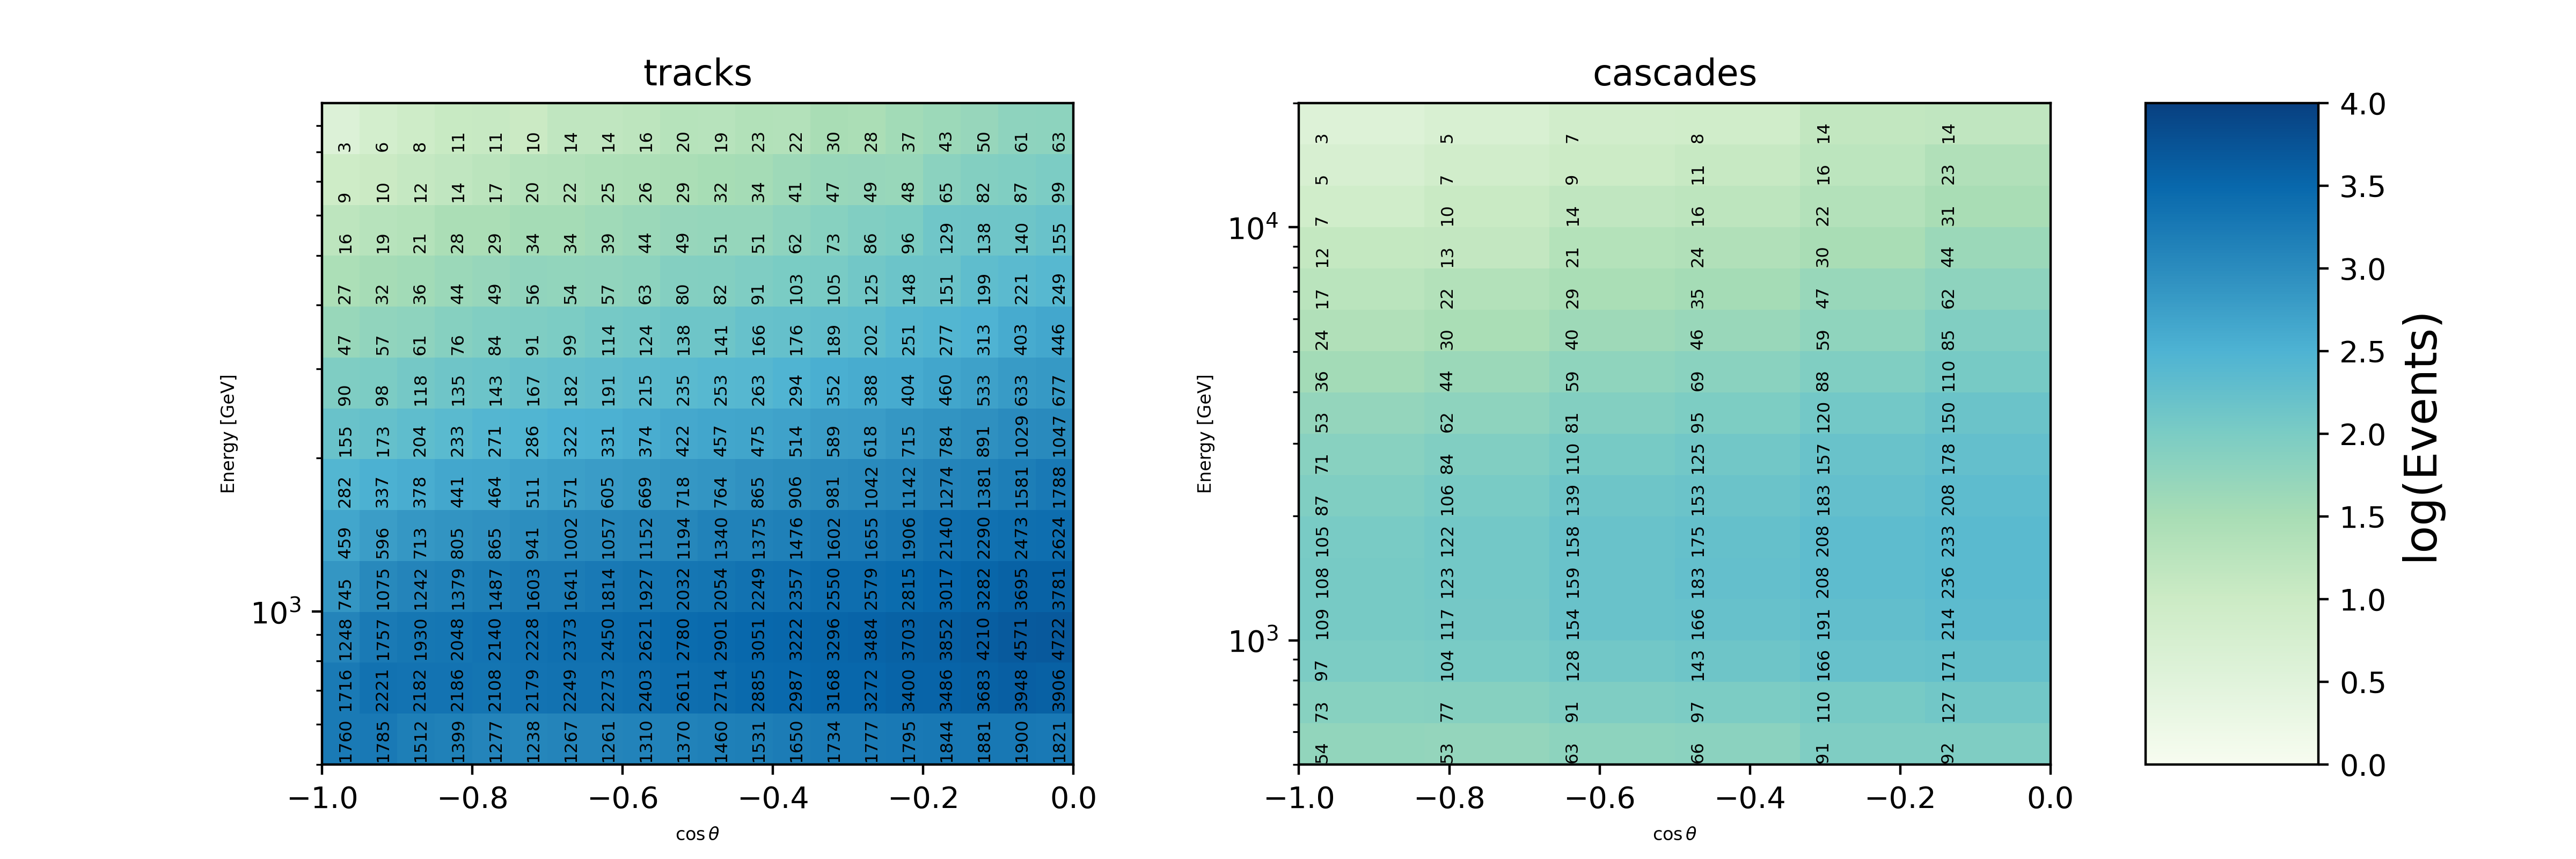
\includegraphics[width=0.8\linewidth]{figures/realization_joint.png}
    \caption{The expected numbers of events in each bin for tracks (left) and cascades (right). Assuming 7.6 years of livetime for tracks and 10 years of livetime for cascades.}\label{fig:event_no}
\end{figure}


\subsection{Track Event Selection}

Since direct neutrino energy reconstruction is impossible for through-going track events, the energy of the muon entering the detector is instead used as a proxy.
The track sample of this analysis uses those events with a muon-proxy energy of between 500 GeV and 10 TeV. 
The event selection is constructed from two sets of cuts, described briefly here, and at length in References~\cite{Aartsen_2020, Aartsen_2020_prd, axani2020sterile}. % 50, 68, 69, 129
The first of these is the ``Golden Filter'':

\begin{enumerate}
    \item Discard events for which fewer than fifteen DOMs are triggered or fewer than six are triggered on direct light.
    \item  For events with $0\leq\cos\theta_{\mu}^{reco}\leq 0.2$, discard if the total charge $Q_{tot}<100$ photoelectrons (PEs) or if the average weighted charge distance $<200$ meters/PE. 
    \item Remove all events with a reconstructed value of $\cos\theta_{\mu}^{reco}\geq 0.2$. This removes down-going track like events that are likely cosmic ray muons. 
    \item Discard all events with a reconstructed track length less than 200 meters, or a track smoothness $<0.6$.
\end{enumerate}

These cuts produce a sample with $\nu_{\mu}$ purity greater than 99\%. %129
An additional ``Diamond filter'' is also used, selecting events after applying these cuts
\begin{enumerate}
    \item Discard events with fewer than twelve direct light DOM triggers. 
    \item Discard events with $Q_{tot}\leq20$ PE outside DeepCore. 
    \item Discard events with fifteen or fewer DOMs triggered outside DeepCore. 
    \item Discard events with $\cos\theta_{\mu}^{reco}>0.05$.
\end{enumerate}
The total track sample is composed of all events which satisfy either the Golden or the Diamond filter. 

With these event selections, strong appearance and disappearance signatures are possible. 
Two possible signatures of sterile neutrino oscillations using these event samples are shown in Figure~\ref{fig:sterile_signature} in analysis space. 

\begin{figure}
    \centering
    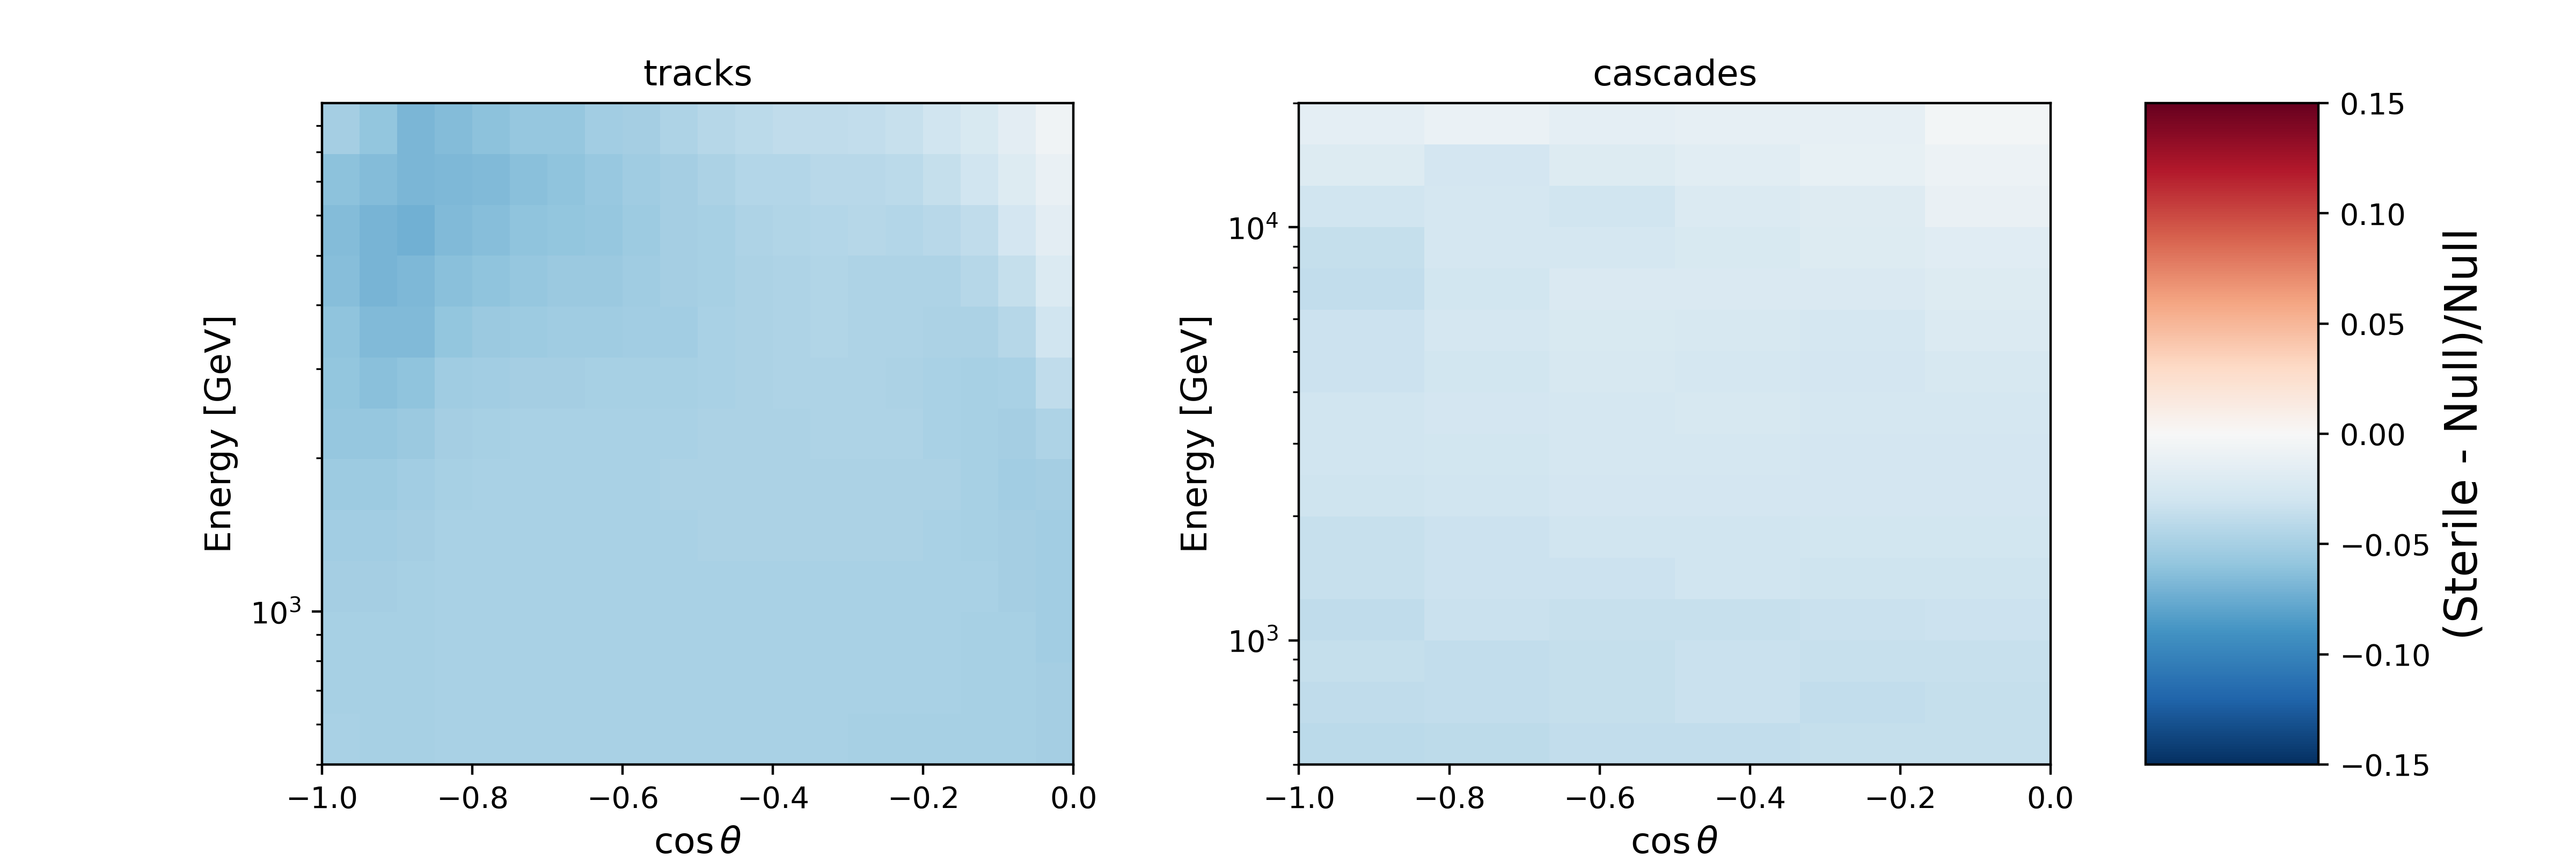
\includegraphics[width=0.85\linewidth]{figures/meows_bf_nofit.png}\\
    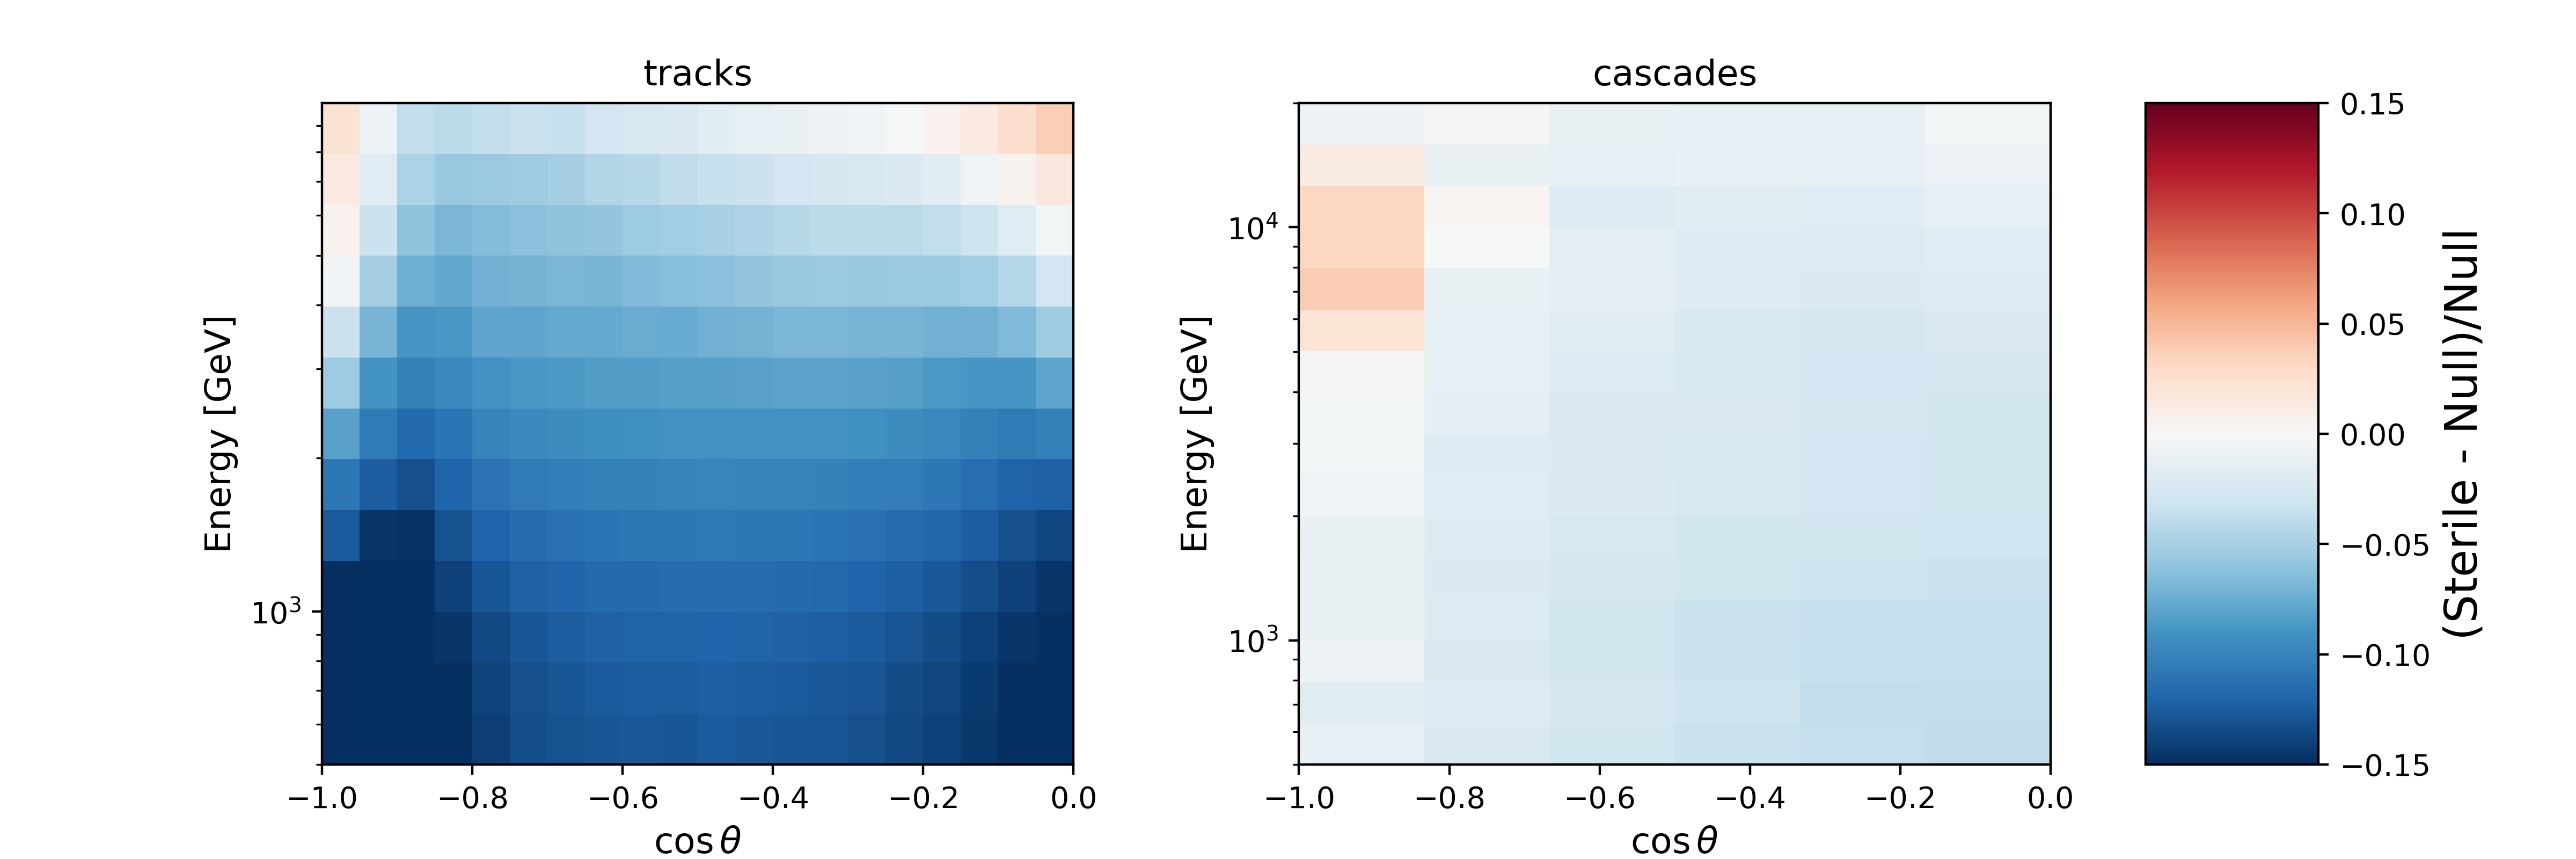
\includegraphics[width=0.85\linewidth]{figures/with_th34_nofit.png}
    \caption{Two signatures of sterile neutrinos in reconstructed space. On the top, the expected disappearance for tracks (left) and cascades (right) for a sterile neutrino model with $\sin^{2}(2\theta_{24})=0.1$ and $\Delta m_{41}^{2}=4.5$ eV$^{2}$. The same is shown on the bottom but with $\sin^{2}(2\theta_{34})=0.05$.}\label{fig:sterile_signature}
\end{figure}

\subsection{Cascade Event Selection}

This final level event filter was developed and published previously for Ref~\cite{2018PhDT17N}.
The likelihood-based reconstruction algorithm monopod is first run on events surviving the level three filter described in Section~\ref{sec:level3};
several quantities are fit and logged including the reconstructed energy, interaction vertex, direction, and a reduced likelihood for the fit (the smaller the reduced log-likelihood is the better).
Events for which the reduced algorithm fail, or which have a reduced log-likelihood (rLogL) of greater than 9.1, are discarded. 
A series of cuts are then applied to reduce the muon contamination: 
\begin{enumerate}
    \item Discard events which are inside the dust layer unless they are high-energy or have rLogl$<7.5$. 
    \item Discard events with a reconstructed vertex with $z$ $>500$ or $z<-500$. 
    \item Discard events which are reconstructed as being near the edge, unless they are well-reconstructed with rLogl$<7.6$.
    \item Discard events near the top or bottom of IceCube unless they are well reconstructed. 
    \item Discard events with very large, negative, photon delay times. This is common for triggers resulting from uncorrelated bundles of atmospheric cosmic ray muons. 
\end{enumerate}
A Boosted Decision Tree classifier is then run on the events which survive these cuts.  
Only those events which satisfy an energy-dependent cut on the cascade score $s_{cascade}$ are kept. The cut is shown below in Figure~\ref{fig:casc_score_cut} and Equation~\eqref{eq:e_casc_cut},
\begin{equation}
    s_{\text{cascade}} > 1 - \left(\dfrac{1}{A + \exp\left[ -B(\log E_{reco} - C) \right]} + D\right),
\end{equation}\label{eq:e_casc_cut}
where the constants $A=1.539$, $B=5$, $C=4.1$, and $D=0.25$.

\begin{figure}
    \centering
    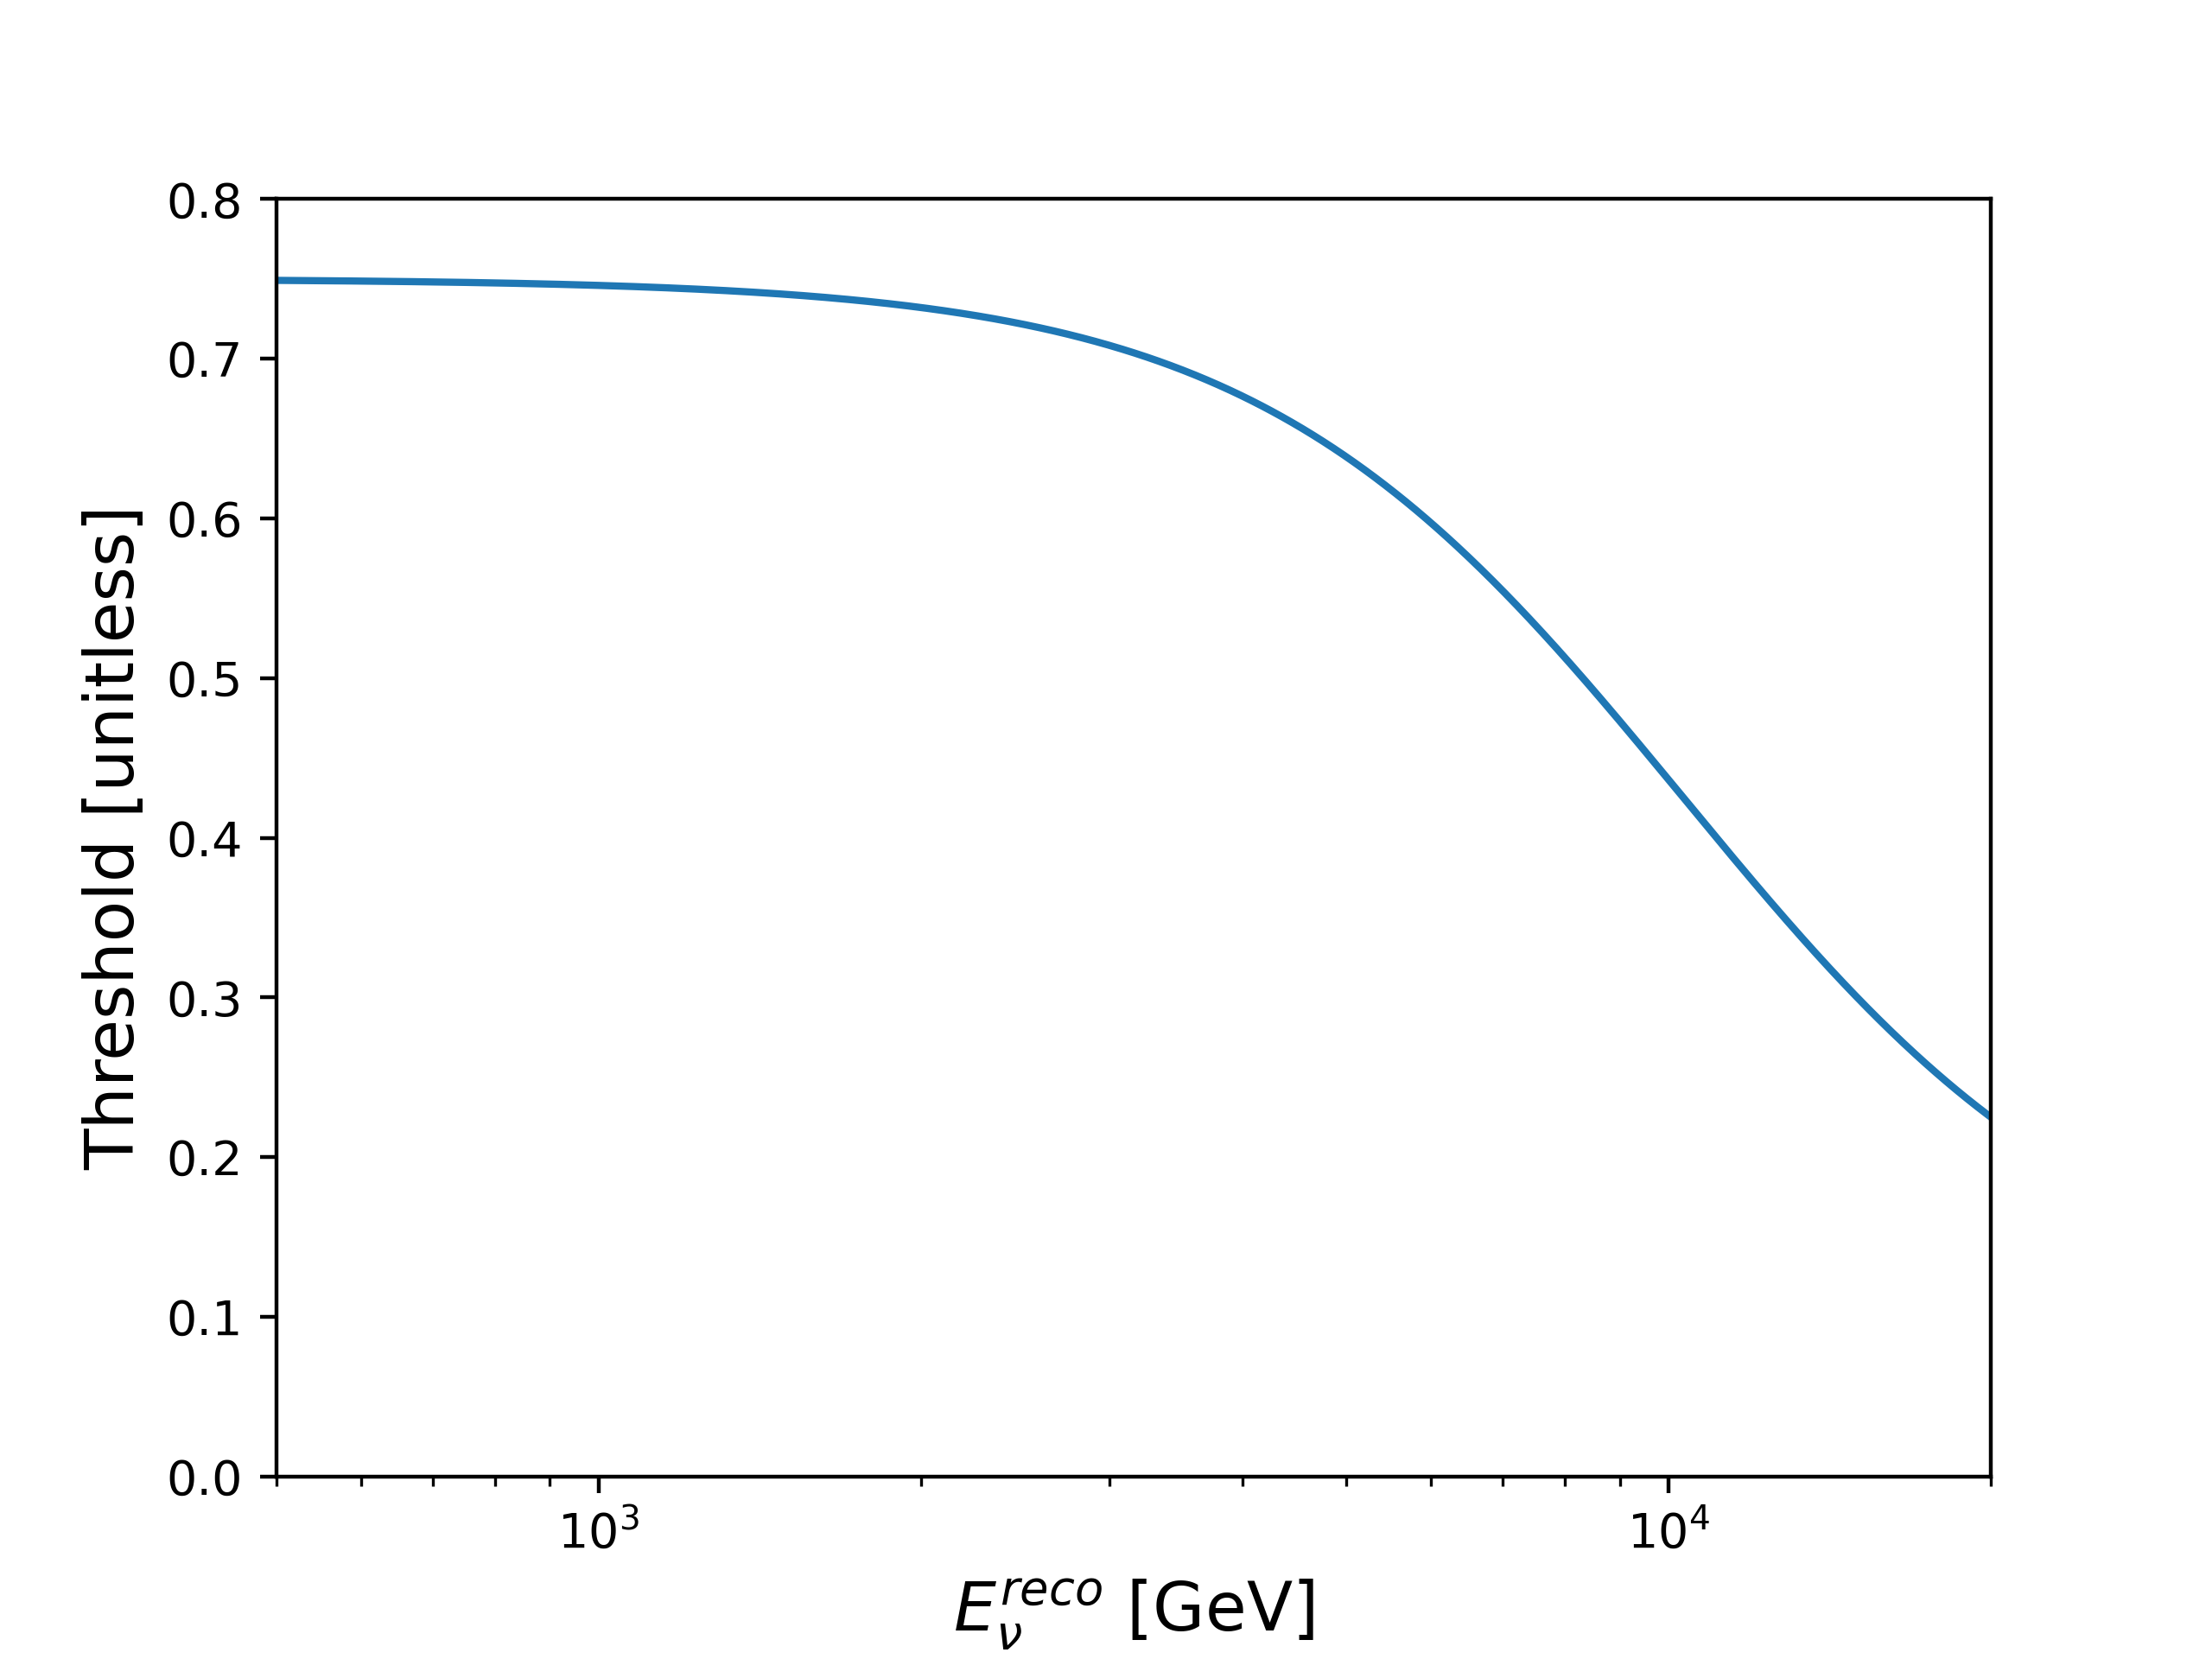
\includegraphics[width=0.6\linewidth]{figures/cut_plot.png}
    \caption{Cascade score $s_{cascade}$ threshold, as a function of energy, below which events are cut.}\label{fig:casc_score_cut}
\end{figure}

\section{Fast Monte Carlo, Event Merging}

For the track sample, around twenty billion MC events were simulated. 
Directly reweighting each of these simulated events for every minimizer step was found to be computationally intractable.
To alleviate these issues, a ``Fast Monte Carlo'' algorithm is used to merge events into meta events, which themselves would be reweighted in fits. 

Events are first weighted according to a flux hypothesis, and the contributions to an event's conventional, prompt, and astrophysical weight are all calculated and stored separately. 
Events are then binned, in reconstructed quantities, into a fine grid whose bin widths are a fraction of the normal analysis bin widths; this fraction is defined as the \textit{fastmode scaling}.
As an example, a fastmode scaling of 0.5 would use twice as many bins along each axis in analysis space\footnote{energy, zenith}, and a scaling of 0.1 would use 10 times as many bins along each axis. 

Events within each of these fine bins are then merged into meta-events; the separate flux-weights are added directly, and a weighted-average is done for analysis quantities like energy and zenith.
The weighted average is calculated according to Equation~\eqref{eq;weighted_fm} for analysis quantity $A$ in fastmode bin $\alpha$.
\begin{equation}\label{eq;weighted_fm}
A_{meta}^{\alpha} = \dfrac{\sum_{i}^{n} A_{\alpha, i} \left(w_{\alpha, i}^{conv} + w_{\alpha,i}^{prompt} + w_{\alpha,i}^{astro}\right) }{\sum_{i}^{n} \left(w_{\alpha, i}^{conv} + w_{\alpha,i}^{prompt} + w_{\alpha,i}^{astro}\right)}
\end{equation}
The sum is carried out over all $n$ events in a fastmode bin. 
These meta-events are then saved with their summed flux-weights and weighted-average analysis quantities.
This procedure is carried out for each tested physics hypothesis, although it is only applied to the track sample. 
A fastmode scaling of 0.1 was used in this analysis and values smaller than 0.25 have been found to produce stable results. 

This Fast Monte Carlo procedure was carried out for all tested physics hypotheses. 

\section{Analysis Test Statistic}\label{sect:llh_metric}

The likelihood $\mathcal{L}(\vec{\Theta}, \vec{\eta})$ used in this analysis is defined as the probability of observing a given set of data, or pseudo-data, assuming some physics hypothesis.
It is quantified as 
\begin{equation}
    \mathcal{L}(\vec{\Theta}, \vec{\eta}) = \prod_{i=0}^{\text{bins}} \mathcal{L}_{eff}\left( w_{i}^{sum}, w_{2,i}^{sum}, k_{i} \right),
\end{equation}
where $w_{i}$ and $w_{2,i}$ are the sums of the MC weights and MC weights squared, respectively, in bin $i$; $k_{i}$ is the observed number of events (or pseudo-events). 
$\vec{\Theta}$ is the tested physics hypothesis and $\vec{\eta}$ the set of nuisance parameters.

The effective likelihood function $\mathcal{L}_{eff}$, defined in Reference~\cite{effective_llh}, is part of a family of likelihood metrics used to account for MC statistical uncertainty. 
We use the form where
\begin{align}
    \alpha&=\dfrac{\mu^{2}}{\sigma^{2}} +1 & &\text{and} & \beta&=\dfrac{\mu}{\sigma^{2}}.
\end{align}
In the case where each MC event is just one event, the mean and variance are defined by $\mu = w_{i}$ and $\sigma^{2} = w_{2,i}$, respectively. For the track sample, meta events are used, and $\sigma^{2} = w_{2,i}/n$, where $n$ is the number of MC events used to generate that meta-event. The effective likelihood function takes the form of 
\begin{equation}
    \mathcal{L}_{eff}(\vec{\Theta} | k) = \left(\dfrac{\mu}{\sigma^{2}}\right)^{\tfrac{\mu^{2}}{\sigma^{2}} + 1} \Gamma\left(k + \dfrac{\mu^{2}}{\sigma^{2}} + 1\right) \left[ k! \left(1+\dfrac{\mu}{\sigma^{2}}\right)^{k+\tfrac{\mu^{2}}{\sigma^{2}} + 1} \Gamma\left(\dfrac{\mu^{2}}{\sigma^{2}} +1\right)\right]^{-1},
\end{equation}
where $\Gamma$ is the gamma function. 

The set of nuisance parameters that quantify systematic uncertainties are themselves constrained by some prior. 
The prior is used to weight the likelihoods which is maximized to form a profile likelihood defined as 
\begin{equation}
\mathcal{L}_{\text{profile}}\left(\vec{\theta}\right) = \text{max}_{\vec{\eta}}\left[\mathcal{L}(\vec{\Theta}, \vec{\eta}) \Xi(\vec{\eta}) \right]
\end{equation}
where $\Xi(\vec{\eta})$ is the total likelihood penalty for the set of nuisance parameters $\vec{\eta}$. We then construct an analysis test statistic (TS) for producing confidence intervals, which we define as 
\begin{equation}\begin{split}
TS(\vec{\Theta}) &= -2\left[ \log\mathcal{L}_{\text{profile}}(\vec{\Theta}) - \log\mathcal{L}_{\text{profile}}(\vec{\Theta}_{min}) \right] \\
 &= -2 \Delta \log\mathcal{L}_{\text{profile}}(\vec{\Theta})\\
&=-2\Delta \text{LLH}
\end{split}\end{equation}
where $\vec{\Theta}_{min}$ is the sterile hypothesis that maximizes the likelihood, and best matches the data (or pseudo-data): the best fit point. 

For fit-scans, we assume that this test statistic satisfies Wilk's Theorem~\cite{10.1214/aoms/1177732360}, and that $\chi^{2}= TS$. 
Threshold values of $\chi^{2}$ for a given number of degrees of freedom $k$ and a desired confidence level $\gamma$ are related by 
\begin{equation}
    \gamma = \dfrac{1}{2^{k/2} \Gamma(k/2)} \int_{0}^{\chi^{2}_{thresh}} dx x^{k/2 - 1} e^{-x/2}. 
\end{equation}
This functional form is inverted to solve for the TS threshold for a given confidence level and number of degrees of fredom. A few example thresholds commonly used here are shown in Table~\ref{table:tsthresh}~\cite{PhysRevD.98.030001}.
\begin{table}
    \centering
    \rowcolors{2}{gray!25}{white}
    \begin{tabular}{c | c c}\rowcolor{blue!25}
        & 2DOF & 3DOF \\\hline
    68\% & 2.72 & 3.51 \\
    90\% & 4.61 & 6.25 \\ 
    95\% & 5.99 & 7.81 \\
    99\% & 9.21 & 11.34 
    \end{tabular}
    \caption{A table listing the test-statistic thresholds assuming Wilk's theorem holds.}\label{table:tsthresh}
\end{table}

\section{Tests}

A series of tests were performed to validate the implementation of the nuisance parameters and verify the performance of the fitting framework. 
Throughout this section, we will refer to two models of the conventional flux: one uses the model from the 8-year sterile neutrino analysis~\cite{Aartsen_2020, Aartsen_2020_prd}; its set of nuisance parameters are listed in Table~\ref{table:nutrition}.
The other model uses the daemonflux~\cite{yanez2023daemonflux} nominal conventional flux model and conventional flux uncertainties ; its set of nuisance parameters are listed in Table~\ref{table:daemon_table}. 
Both were investigated and in the process we found that the 8-year analysis model could yield spurious 3+1 signatures following a mismodeling of the conventional neutrino flux. 
Since Daemonflux was found to the model less likely to yield spurious signals of sterile neutrinos, it was used as the nominal model for fits to the data.

\subsection{Previous Results Cross-Check}

First we verified we could recover the same sensitivities as from the original eight-year analysis, whose sensitivities are published in References~\cite{Aartsen_2020} and~\cite{Aartsen_2020_prd}.

New fluxes, gradients, and Fast MC, were generated in logarithmic steps in $\sin^{2}(2\theta_{24})$ and $\Delta m_{41}^{2}$ space using the same techniques as what are used for the joint fits over ($\Delta m_{41}^{2}$, $\abs{U_{\mu 4}}^{2}$, $\abs{U_{\tau 4}}^{2}$).
Using the new PISA framework, we ran a global-scan of nuisance parameter fits to an Asimov realization: the nominal expectation of the experiment without nuisance parameter or statistical fluctuations.
The resulting 90\% confidence level sensitivities from the track sample alone are shown in Figure~\ref{fig:comparison} alongside the sensitivities from the 8-year analysis. 
From this we conclude that the new fitting implementation in PISA is valid and can be used. 

\begin{figure}
    \centering
    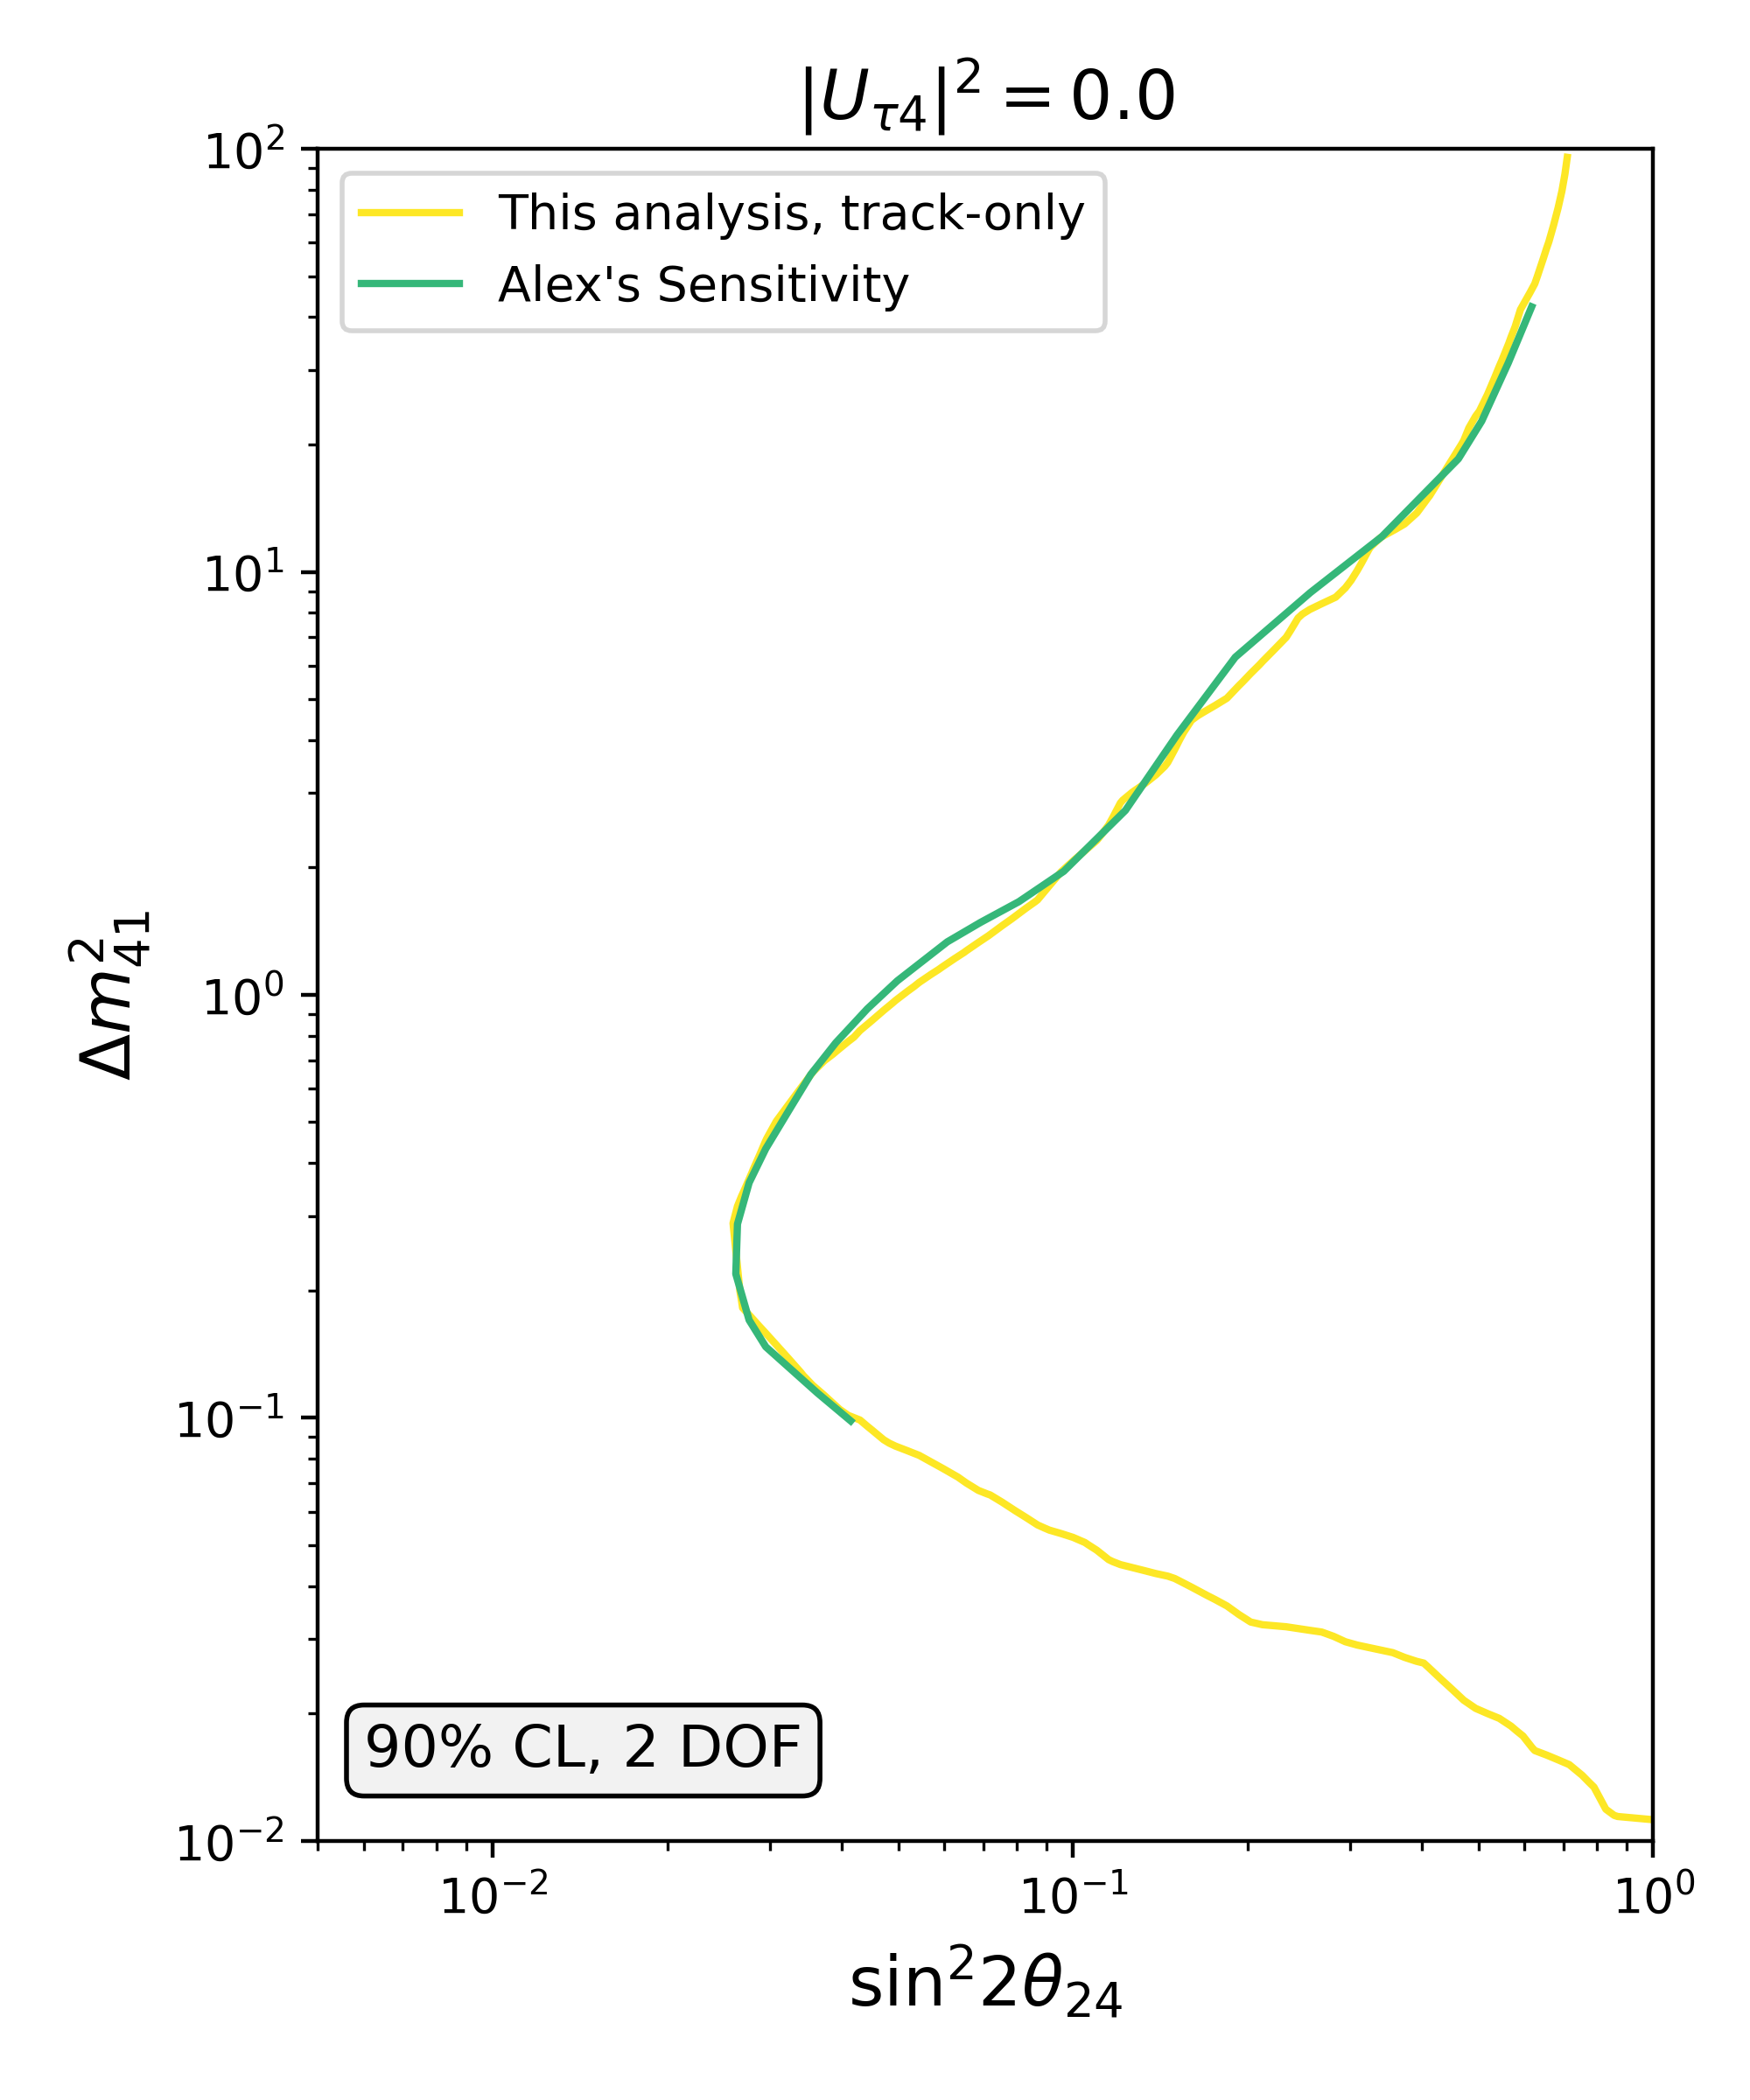
\includegraphics[width=0.6\linewidth]{figures/track_asimov_oldairs_Realization_Asimov_sterile_0_cl0.9_dof2.png}
    \caption{The 90\% CL sensitivity contours for two degrees of freedom, using only the track sample, as determined for this analysis (yellow) and the original 8-year tracks sample (green).}\label{fig:comparison}
\end{figure}

\subsection{Inject-Recover Systematic Tests}

Pseudo-experimental results, or `realizations,' are generated by perturbing all nuisance parameters according to their priors, simultaneously, and saving the expected event rates without additional statistical variation applied. 
Fits are then carried out to each of these realizations.

The results are tabulated in two figures where the true injected and recovered values are shown: in Figure~\ref{fig:ir_nopriorpert} the fits are kept with the priors' centers kept at their original value, and in Figure~\ref{fig:ir_priorpert} the priors are changed to the value of the injected nuisance parameter. 
In Figure~\ref{fig:ir_nopriorpert}, the flatter the trend is then the more tightly-constrained its prior is compared to the shape effects caused by the nuisance parameter itself; in Figure~\ref{fig:ir_priorpert}, the injected values are all recovered exactly. 
We conclude that the minimization framework successfully recovers the true minimum in fits. 

\begin{figure}
    \centering 
    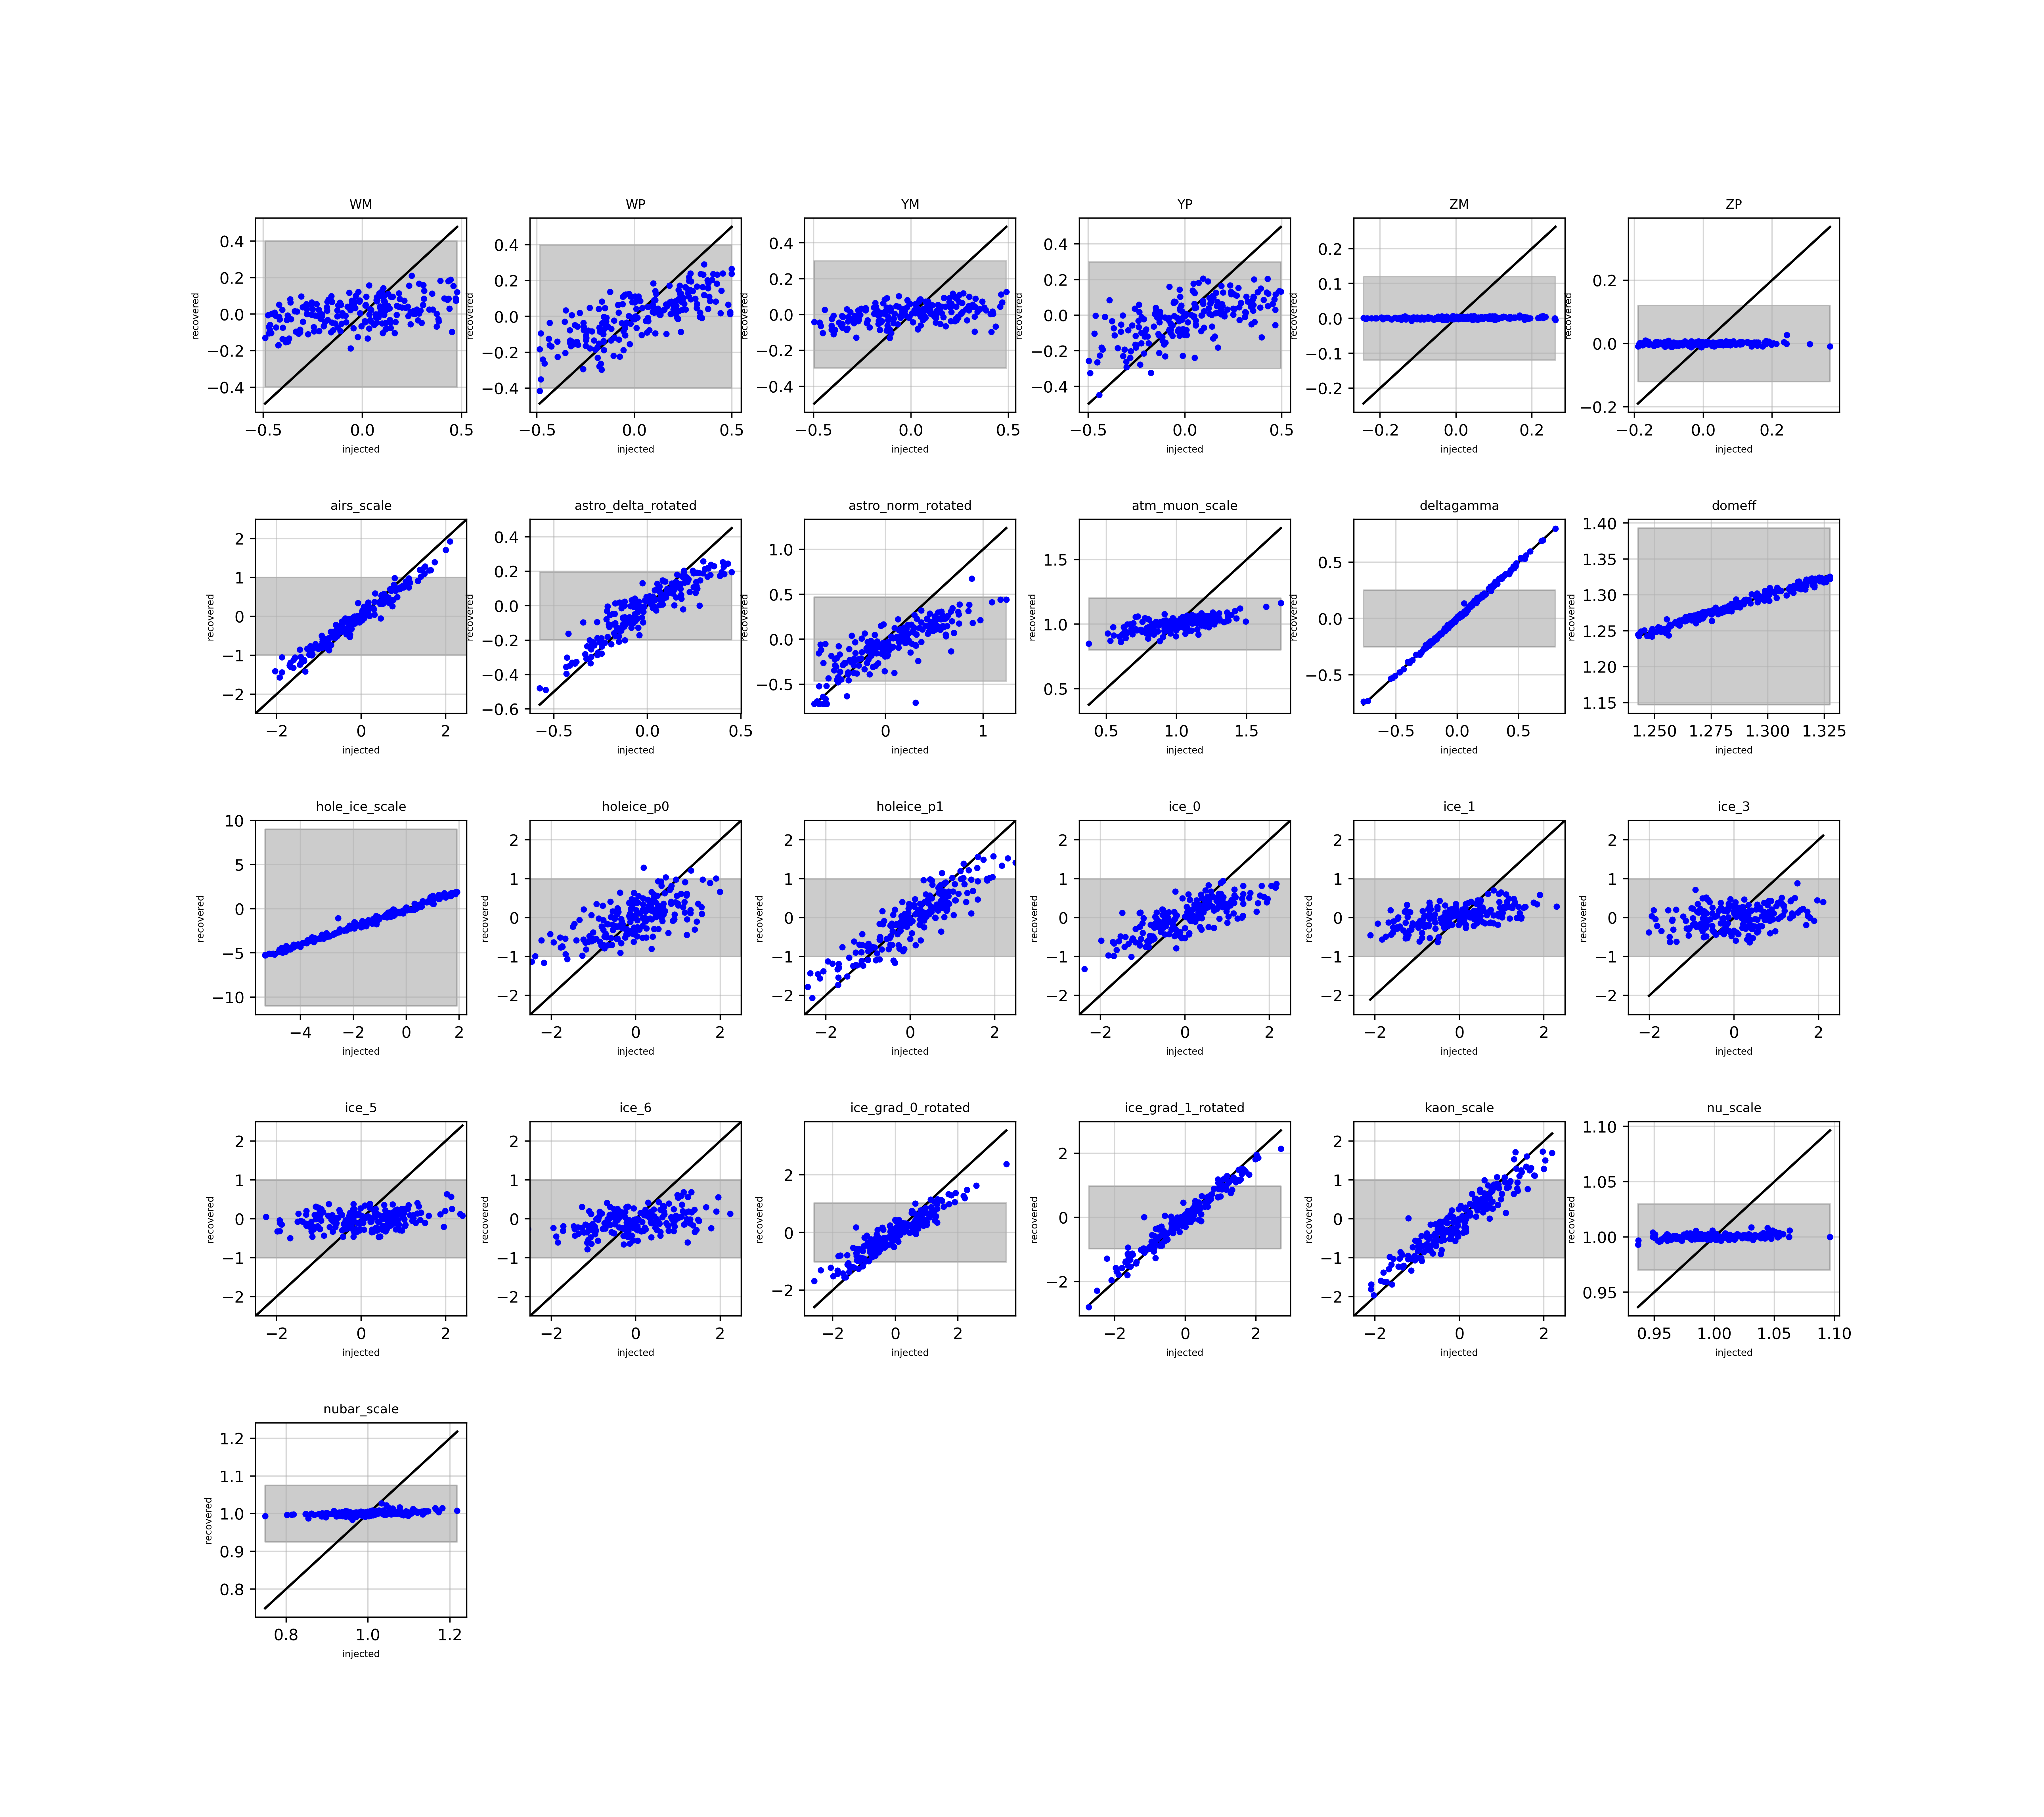
\includegraphics[width=0.7\linewidth]{figures/syst_ir_shuffle_nofix.png}
    \caption{Fit results after injecting various perturbed values for each nuisance parameter and running the fitter. A shaded gray region demonstrates the $1\sigma$ prior width on the nuisance parameter's prior.}\label{fig:ir_nopriorpert}
\end{figure}


\begin{figure}
    \centering 
    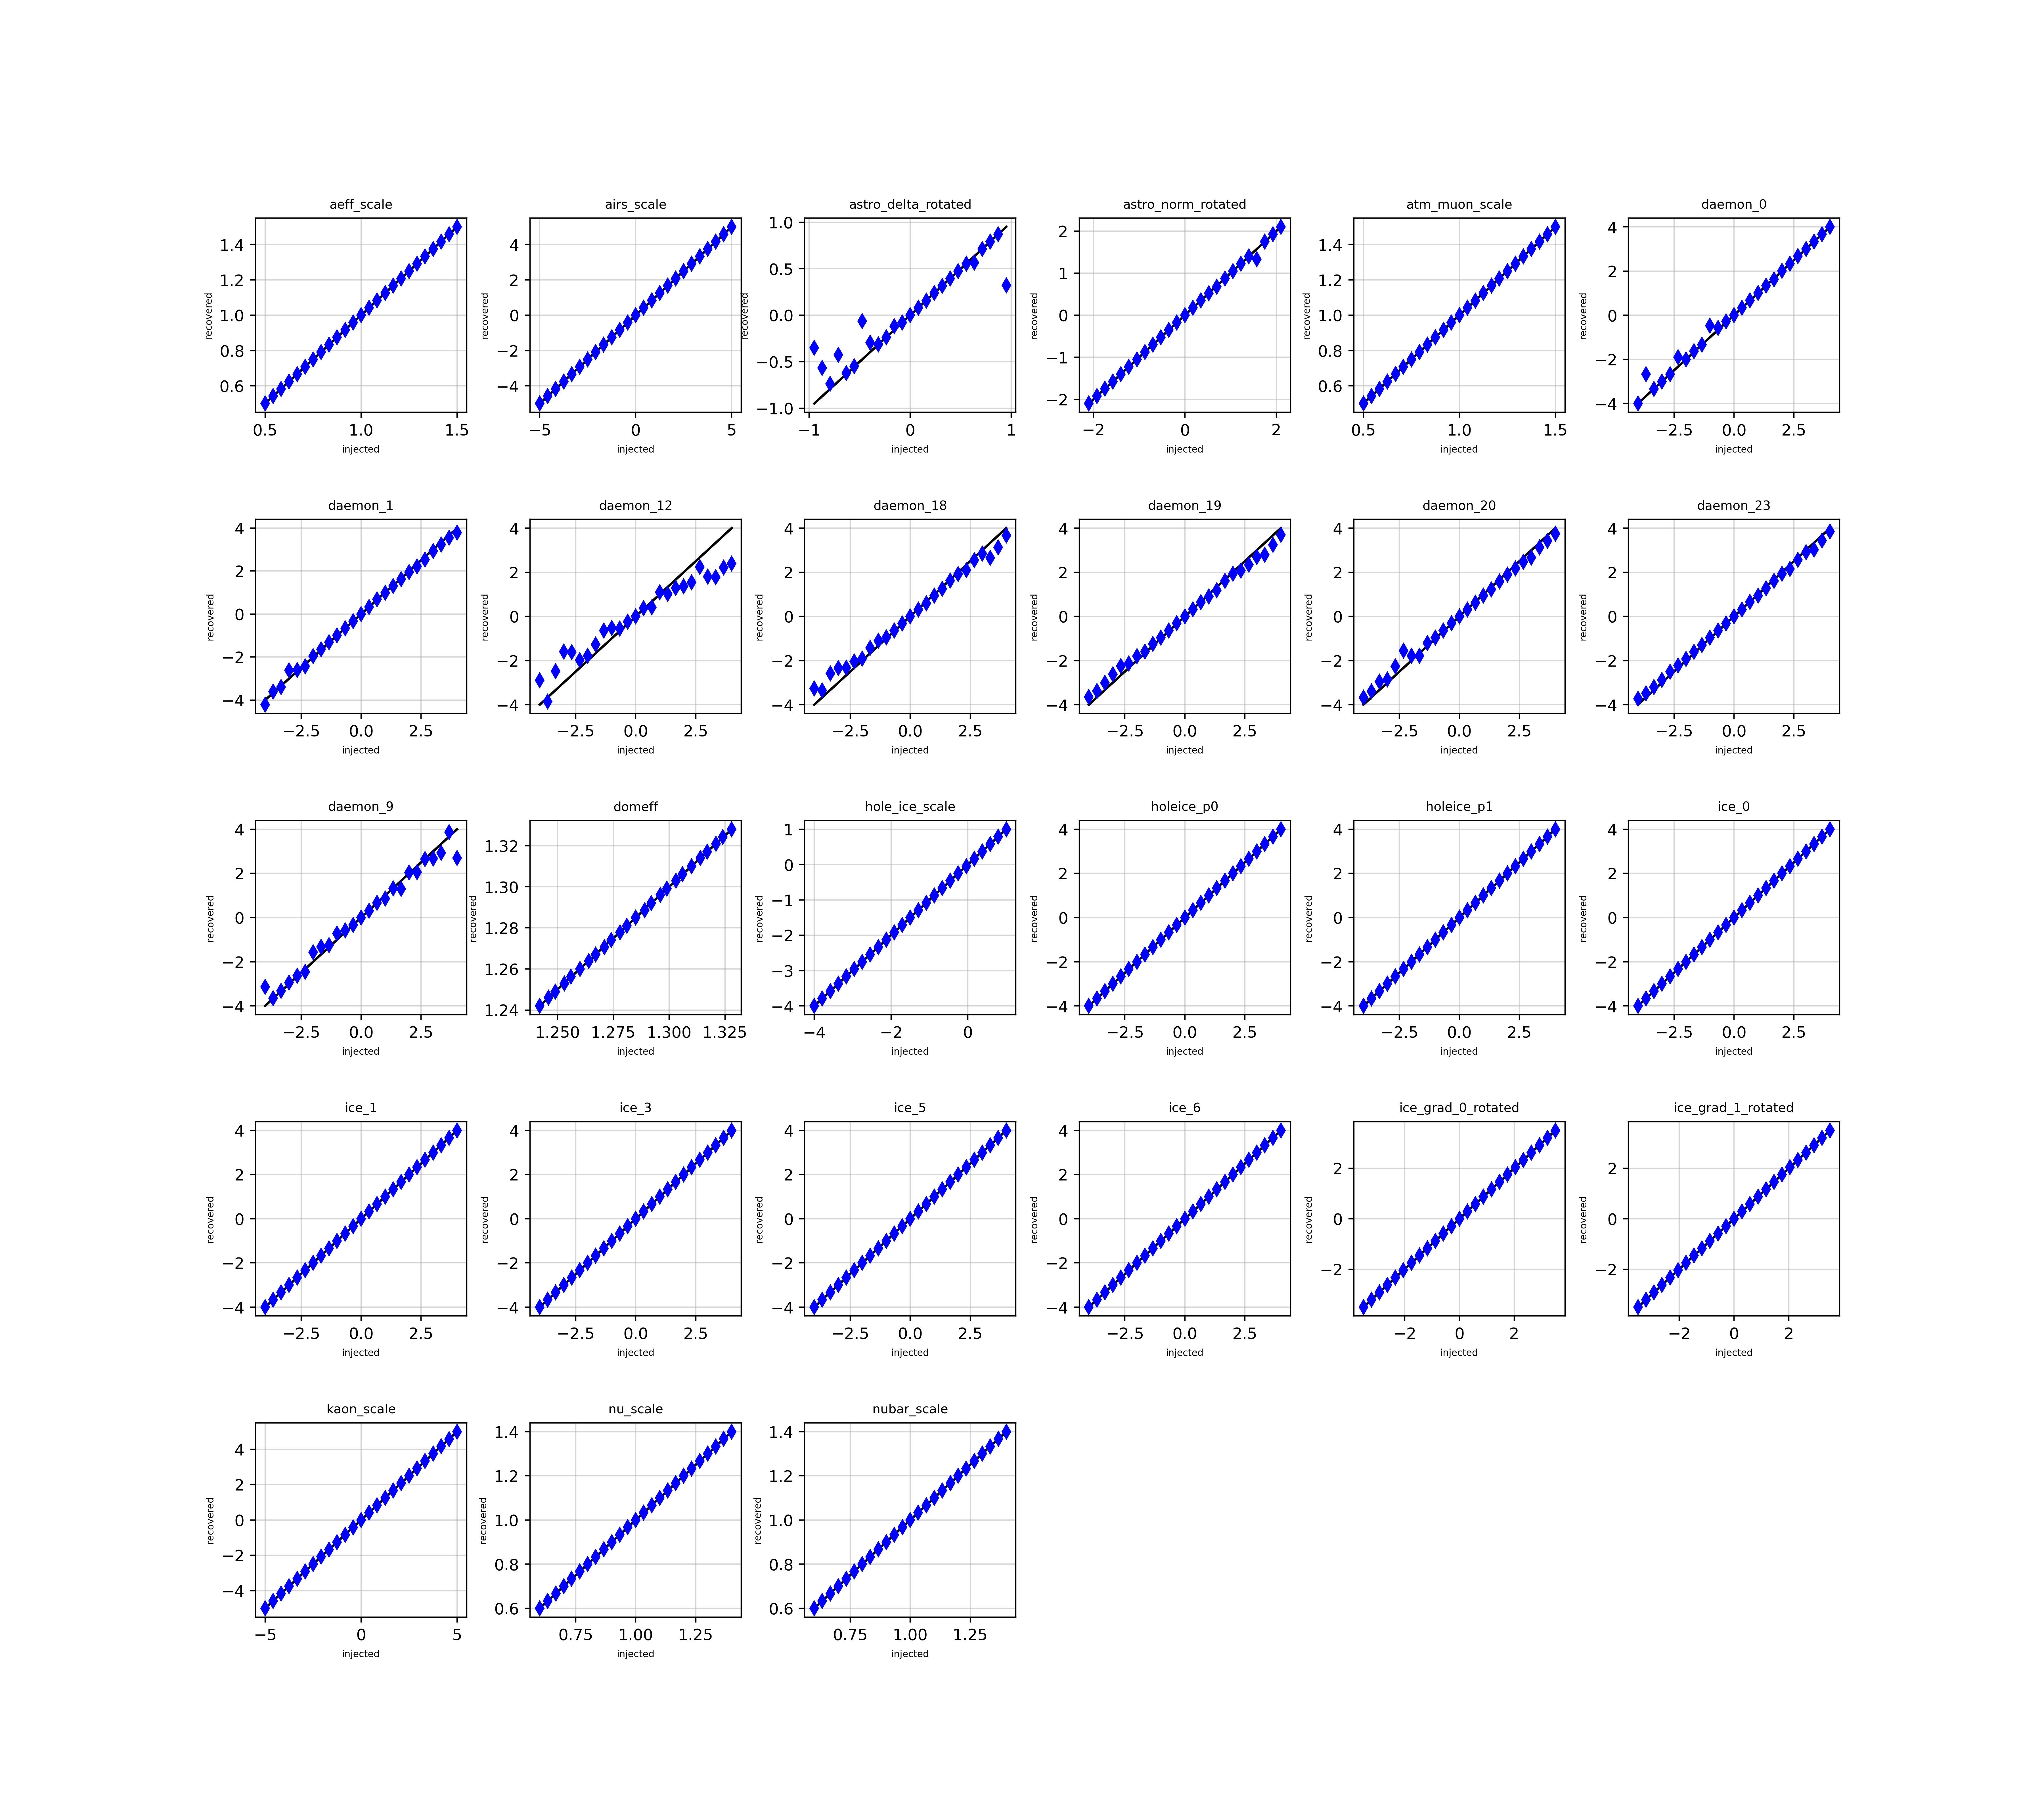
\includegraphics[width=0.7\linewidth]{figures/update_inject_recover_syst_prior.png}
    \caption{Fit results after injecting various perturbed values for each nuisance parameter and running the fitter. Priors are adjusted in each fit according to the injected values.}\label{fig:ir_priorpert}
\end{figure}

\subsection{Systematic Impact Tests}

Another test was done to characterize how strongly each nuisance parameter, or set thereof, effects overall sensitivity. 
Nuisance parameters were collected into ``bundles,'' and Asimov sensitivity scans~\cite{Cowan_2011} were performed while fixing all nuisance parameters of that bundle to their central values.
The constraints, compared to the full fits, show the impact of fixing those nuisance parameters. 
The bundles are 
\begin{enumerate}
    \item Norm(alization): everything is fixed except for the normalization.
    \item Astro(physical): astrophysical normalization and the spectral index
    \item Conv(entional): Daemonflux~\cite{yanez2023daemonflux} parameters, Barr parameters, AIRS scale, and the kaon-nucleon cross-section uncertainty
    \item Det(ector): hole ice uncertainty, DOM efficiency, and the bulk-ice uncertainty
    \item Muon: the CR muon background\footnote{Because of the large, extra, error introduced by the muon background, for this systematic impact test a special realization is generated and fit to where there no muon contribution is added at all.}
\end{enumerate}
The systematic impact tests were calculated twice for the two conventional flux models: once using the model from the previous 8-year analysis, and once using daemonflux. 
Both are shown at 90\% confidence level and with three degrees of freedom in Figure~\ref{fig:impact}. 
For both models we find that the conventional flux uncertainty has the strongest effect on our sensitivity while the detector systematic uncertainties have the second strongest effect. 

\begin{figure}
    \centering
    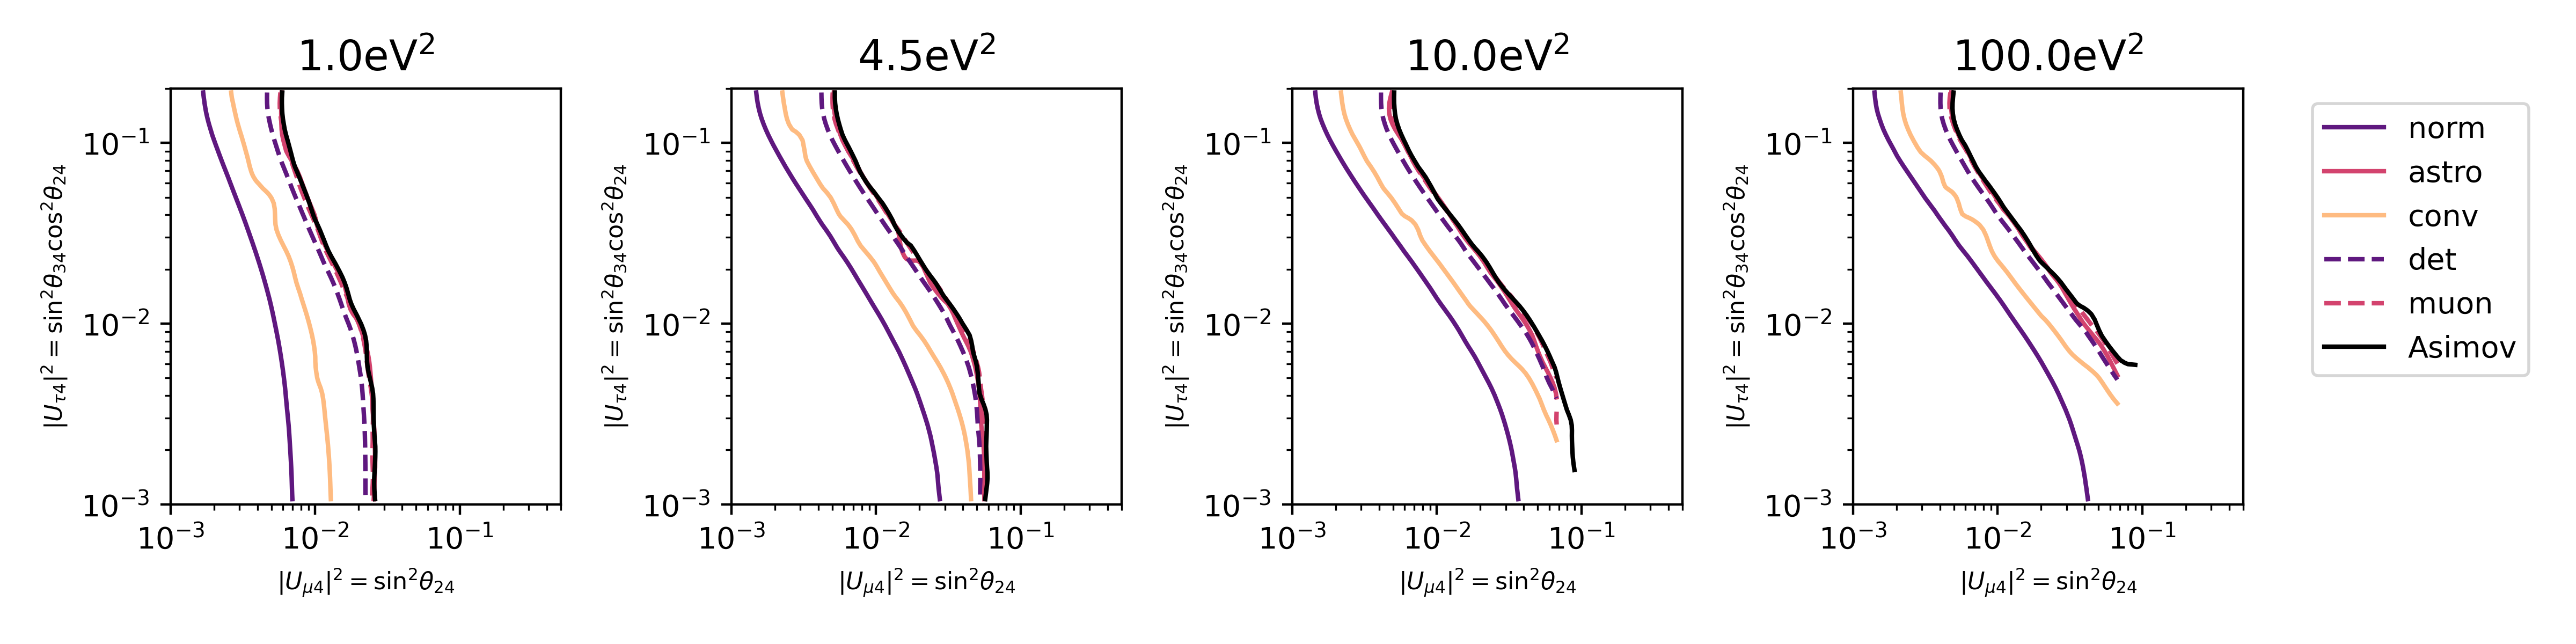
\includegraphics[width=0.95\linewidth]{figures/systematic_impact_joint.png}\\
    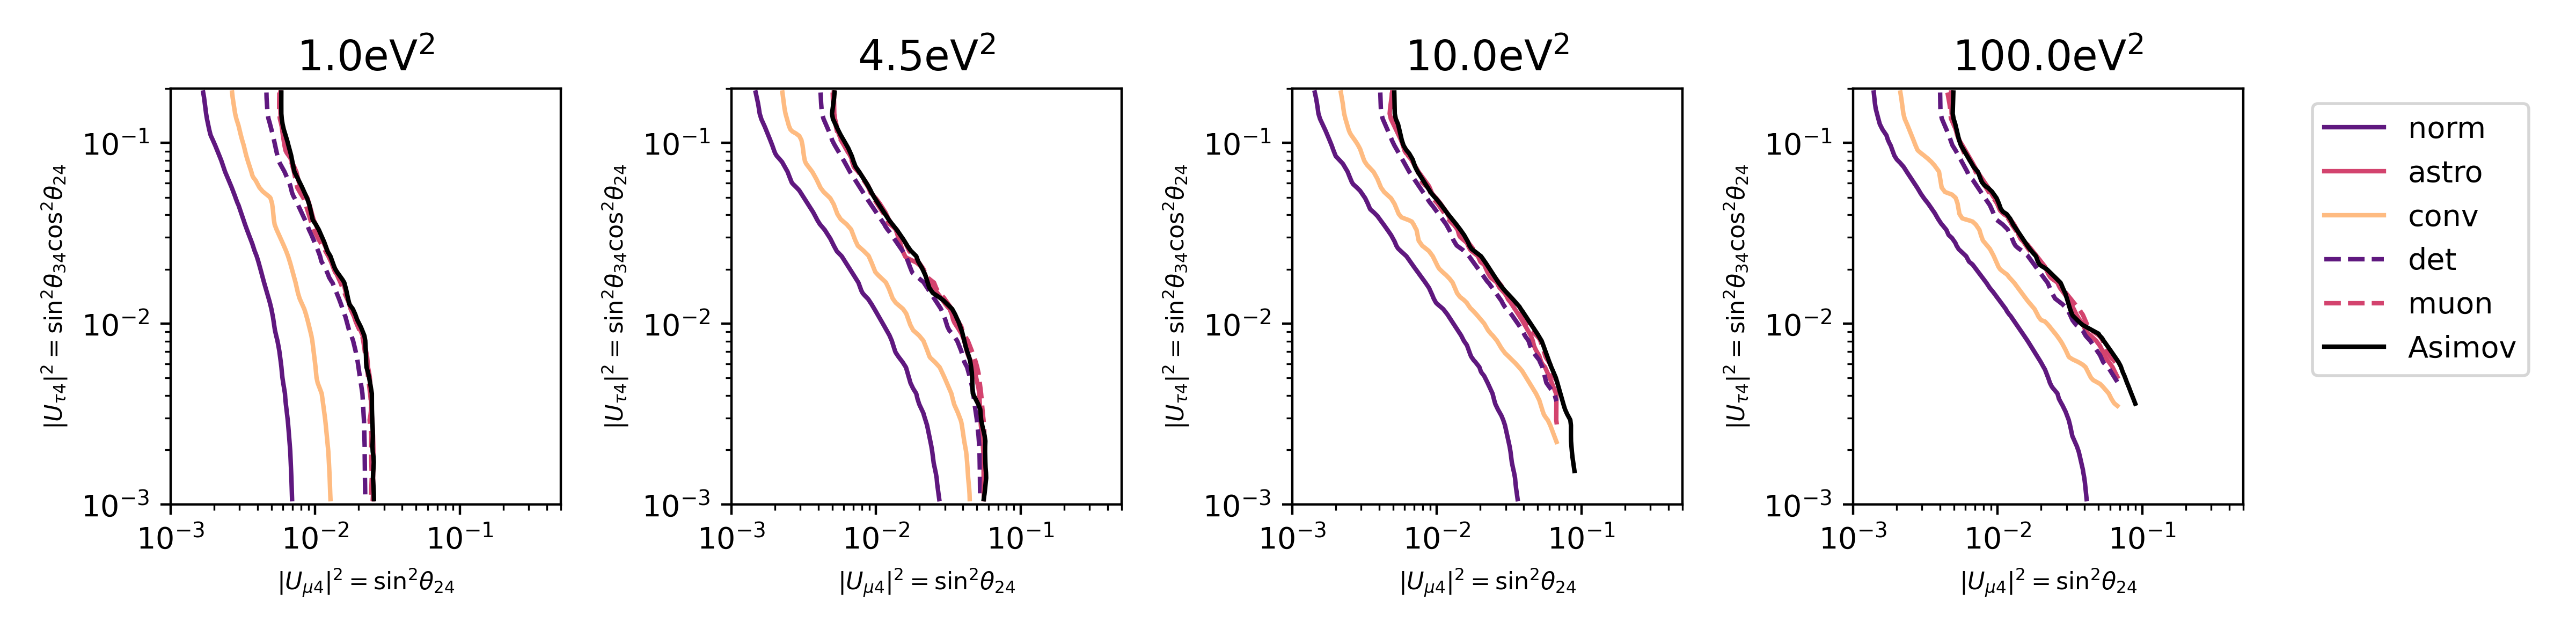
\includegraphics[width=0.95\linewidth]{figures/Systematic_impact_joint_daemon.png}
    \caption{The sensitivity contours for fixing each bundle of nuisance parameters. Contours are shown at 90\% CL and 3DOF for various mass-squared splittings; from left to right: 1.0eV$^{2}$, 4.5eV$^{2}$, 10.0eV$^{2}$, and 100.0eV$^{2}$. Top: results when using the conventional flux model used in the 8-year analysis, and on bottom: the results when using daemonflux.}\label{fig:impact}
\end{figure}

\subsection{Signal Inject-Recover}

Various points were chosen along the Asimov 90\% CL thresholds to test the fitting framework's ability to recover constraints of sterile-neutrino signal-like measurements. 
Two each were chosen along the contours at 1.0, 4.5, and 10 eV$^{2}$; one more was chosen at 100 eV$^{2}$. 
Additionally, three more points were chosen off-grid at various points.
Of those three, one was selected as the recovered best-fit point from the 8-year track analysis. 
Then, we ran a full fit-scan on an Asimov realization generated for each of these simulated signals. 
Injected values are recovered in all cases where a signal is injected at a grid-point.
For the cases where a signal is injected near a grid point, the recovered best fit is sufficiently close, 
and we find that the minimizer is able to accurately recover an injected 3+1 signal. 
Exclusion contours for these signal inject-recover tests are shown in Figures~\ref{fig:first_ir} through~\ref{fig:last_ir}.

\begin{figure}
    \centering
    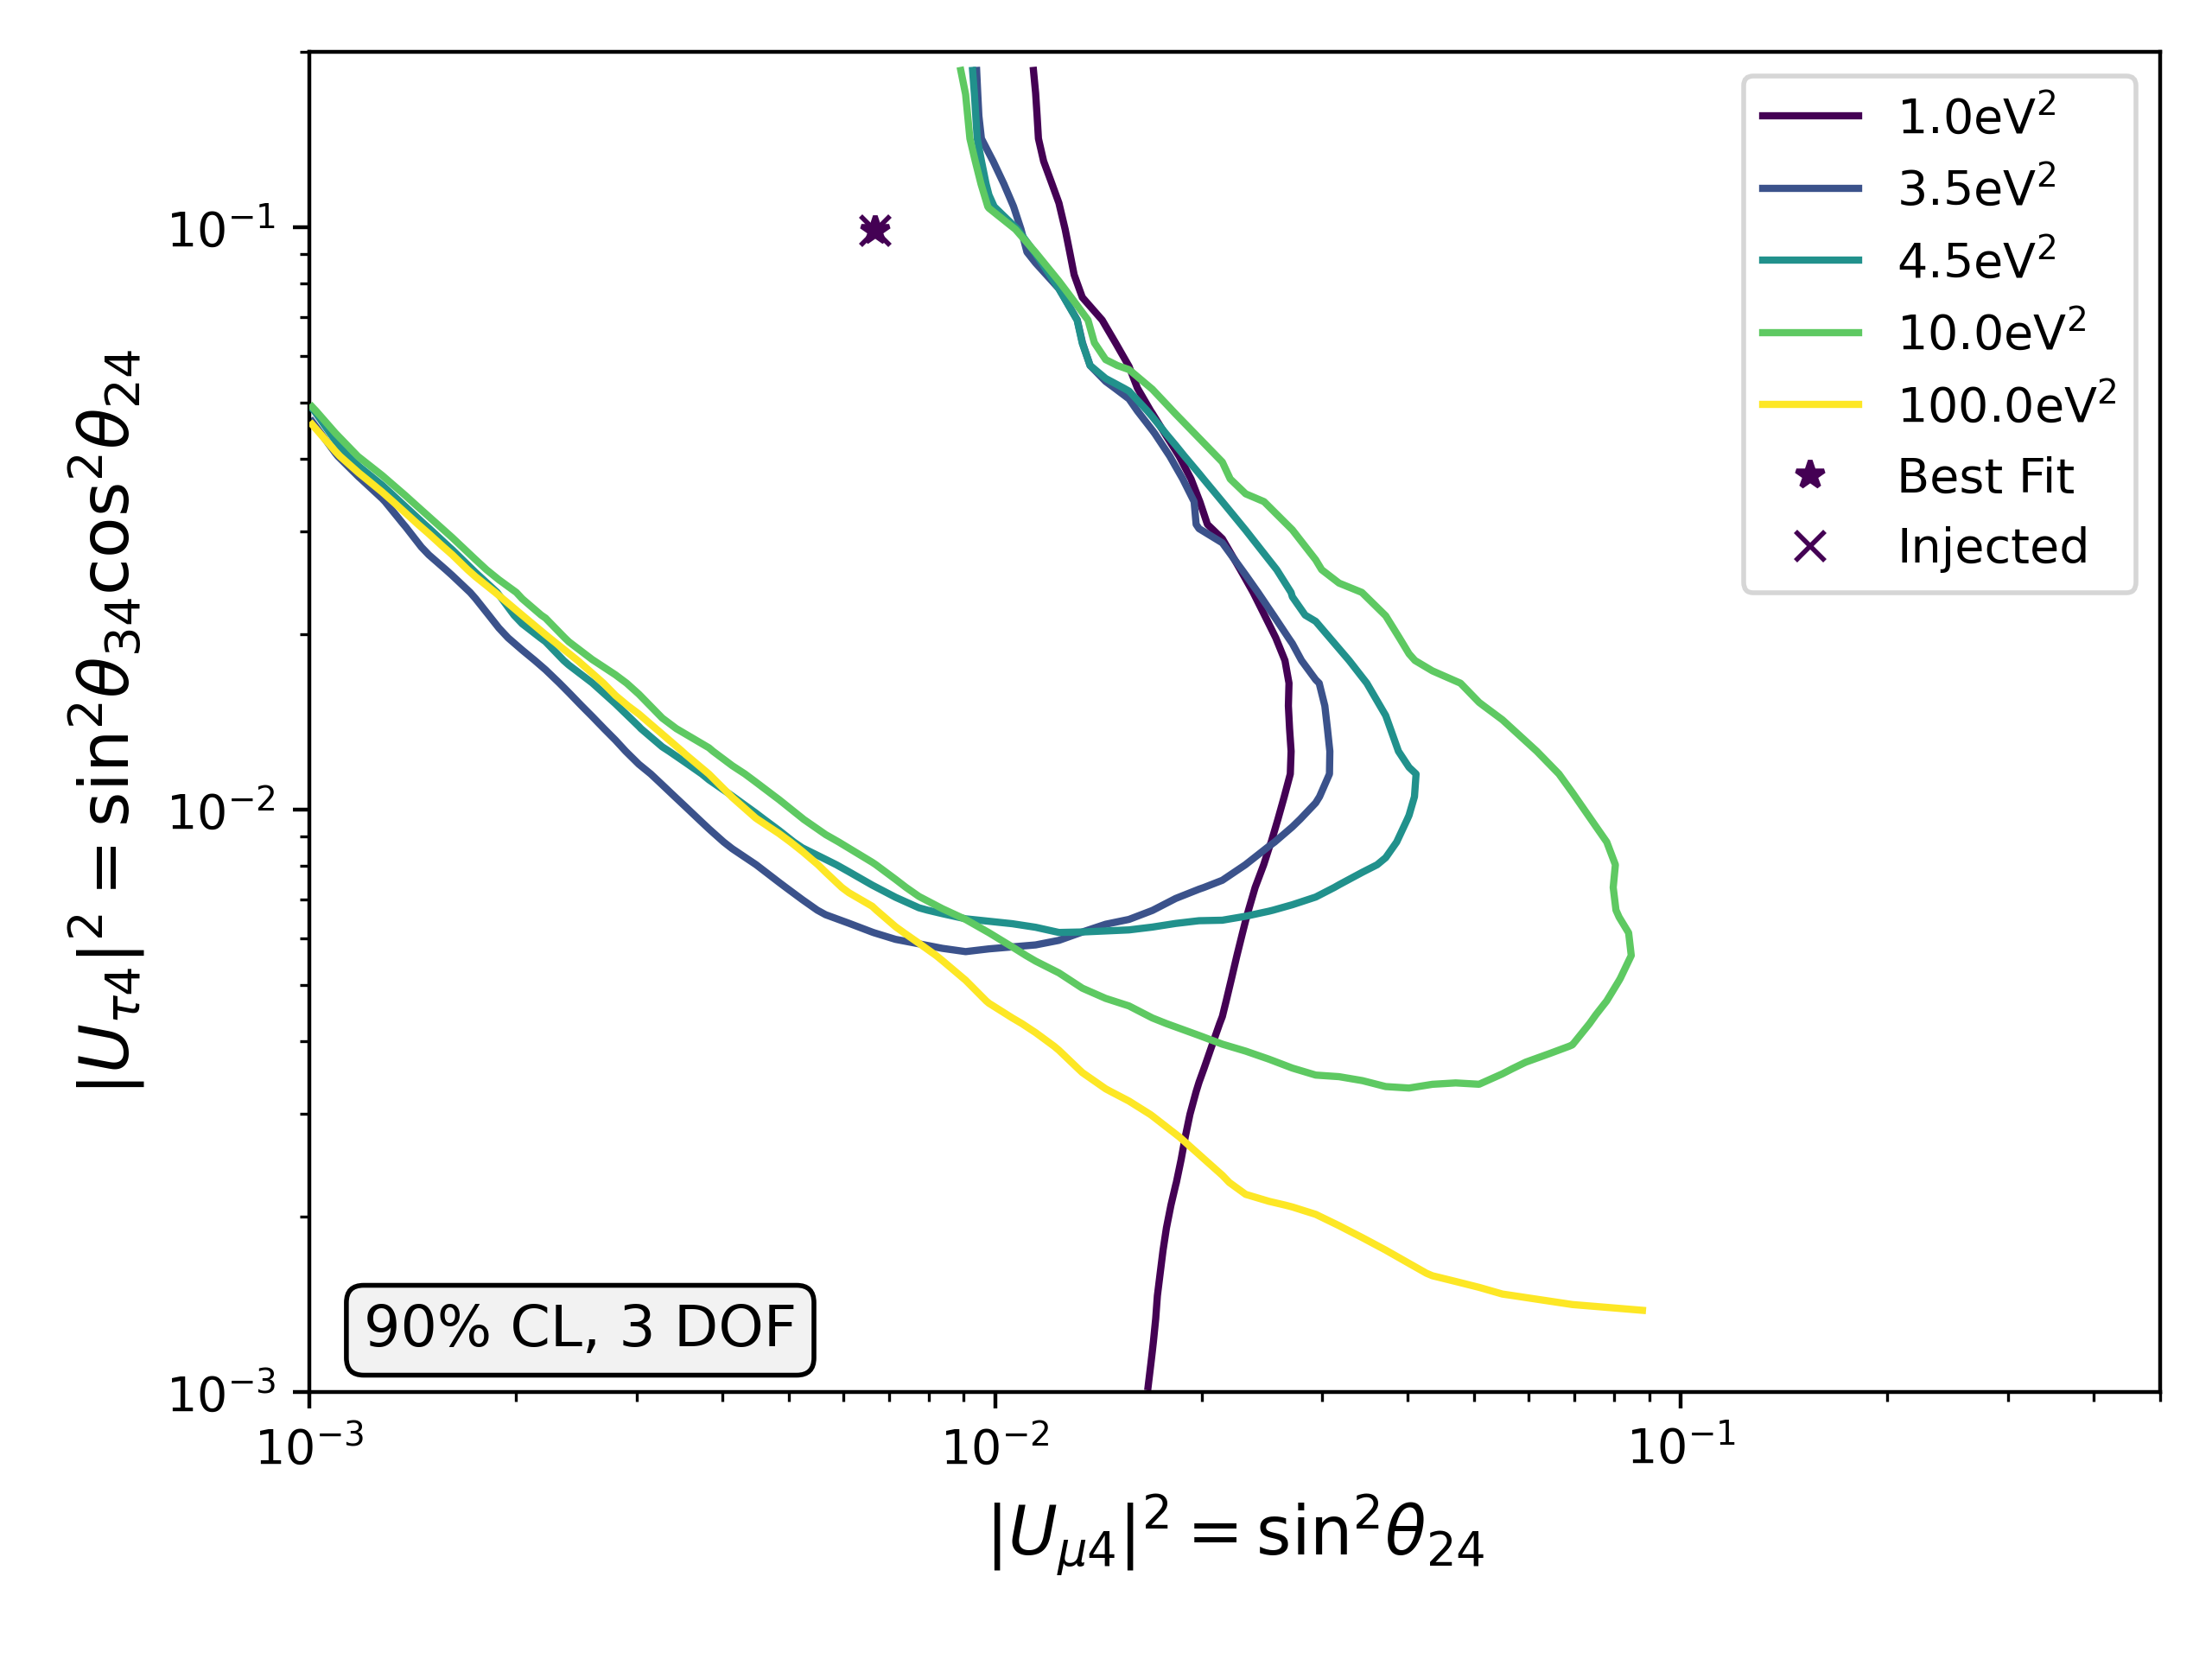
\includegraphics[width=0.45\linewidth]{figures/inject_recover_RealIR_0_sterile_1_cl0.9_dof3.png}%
    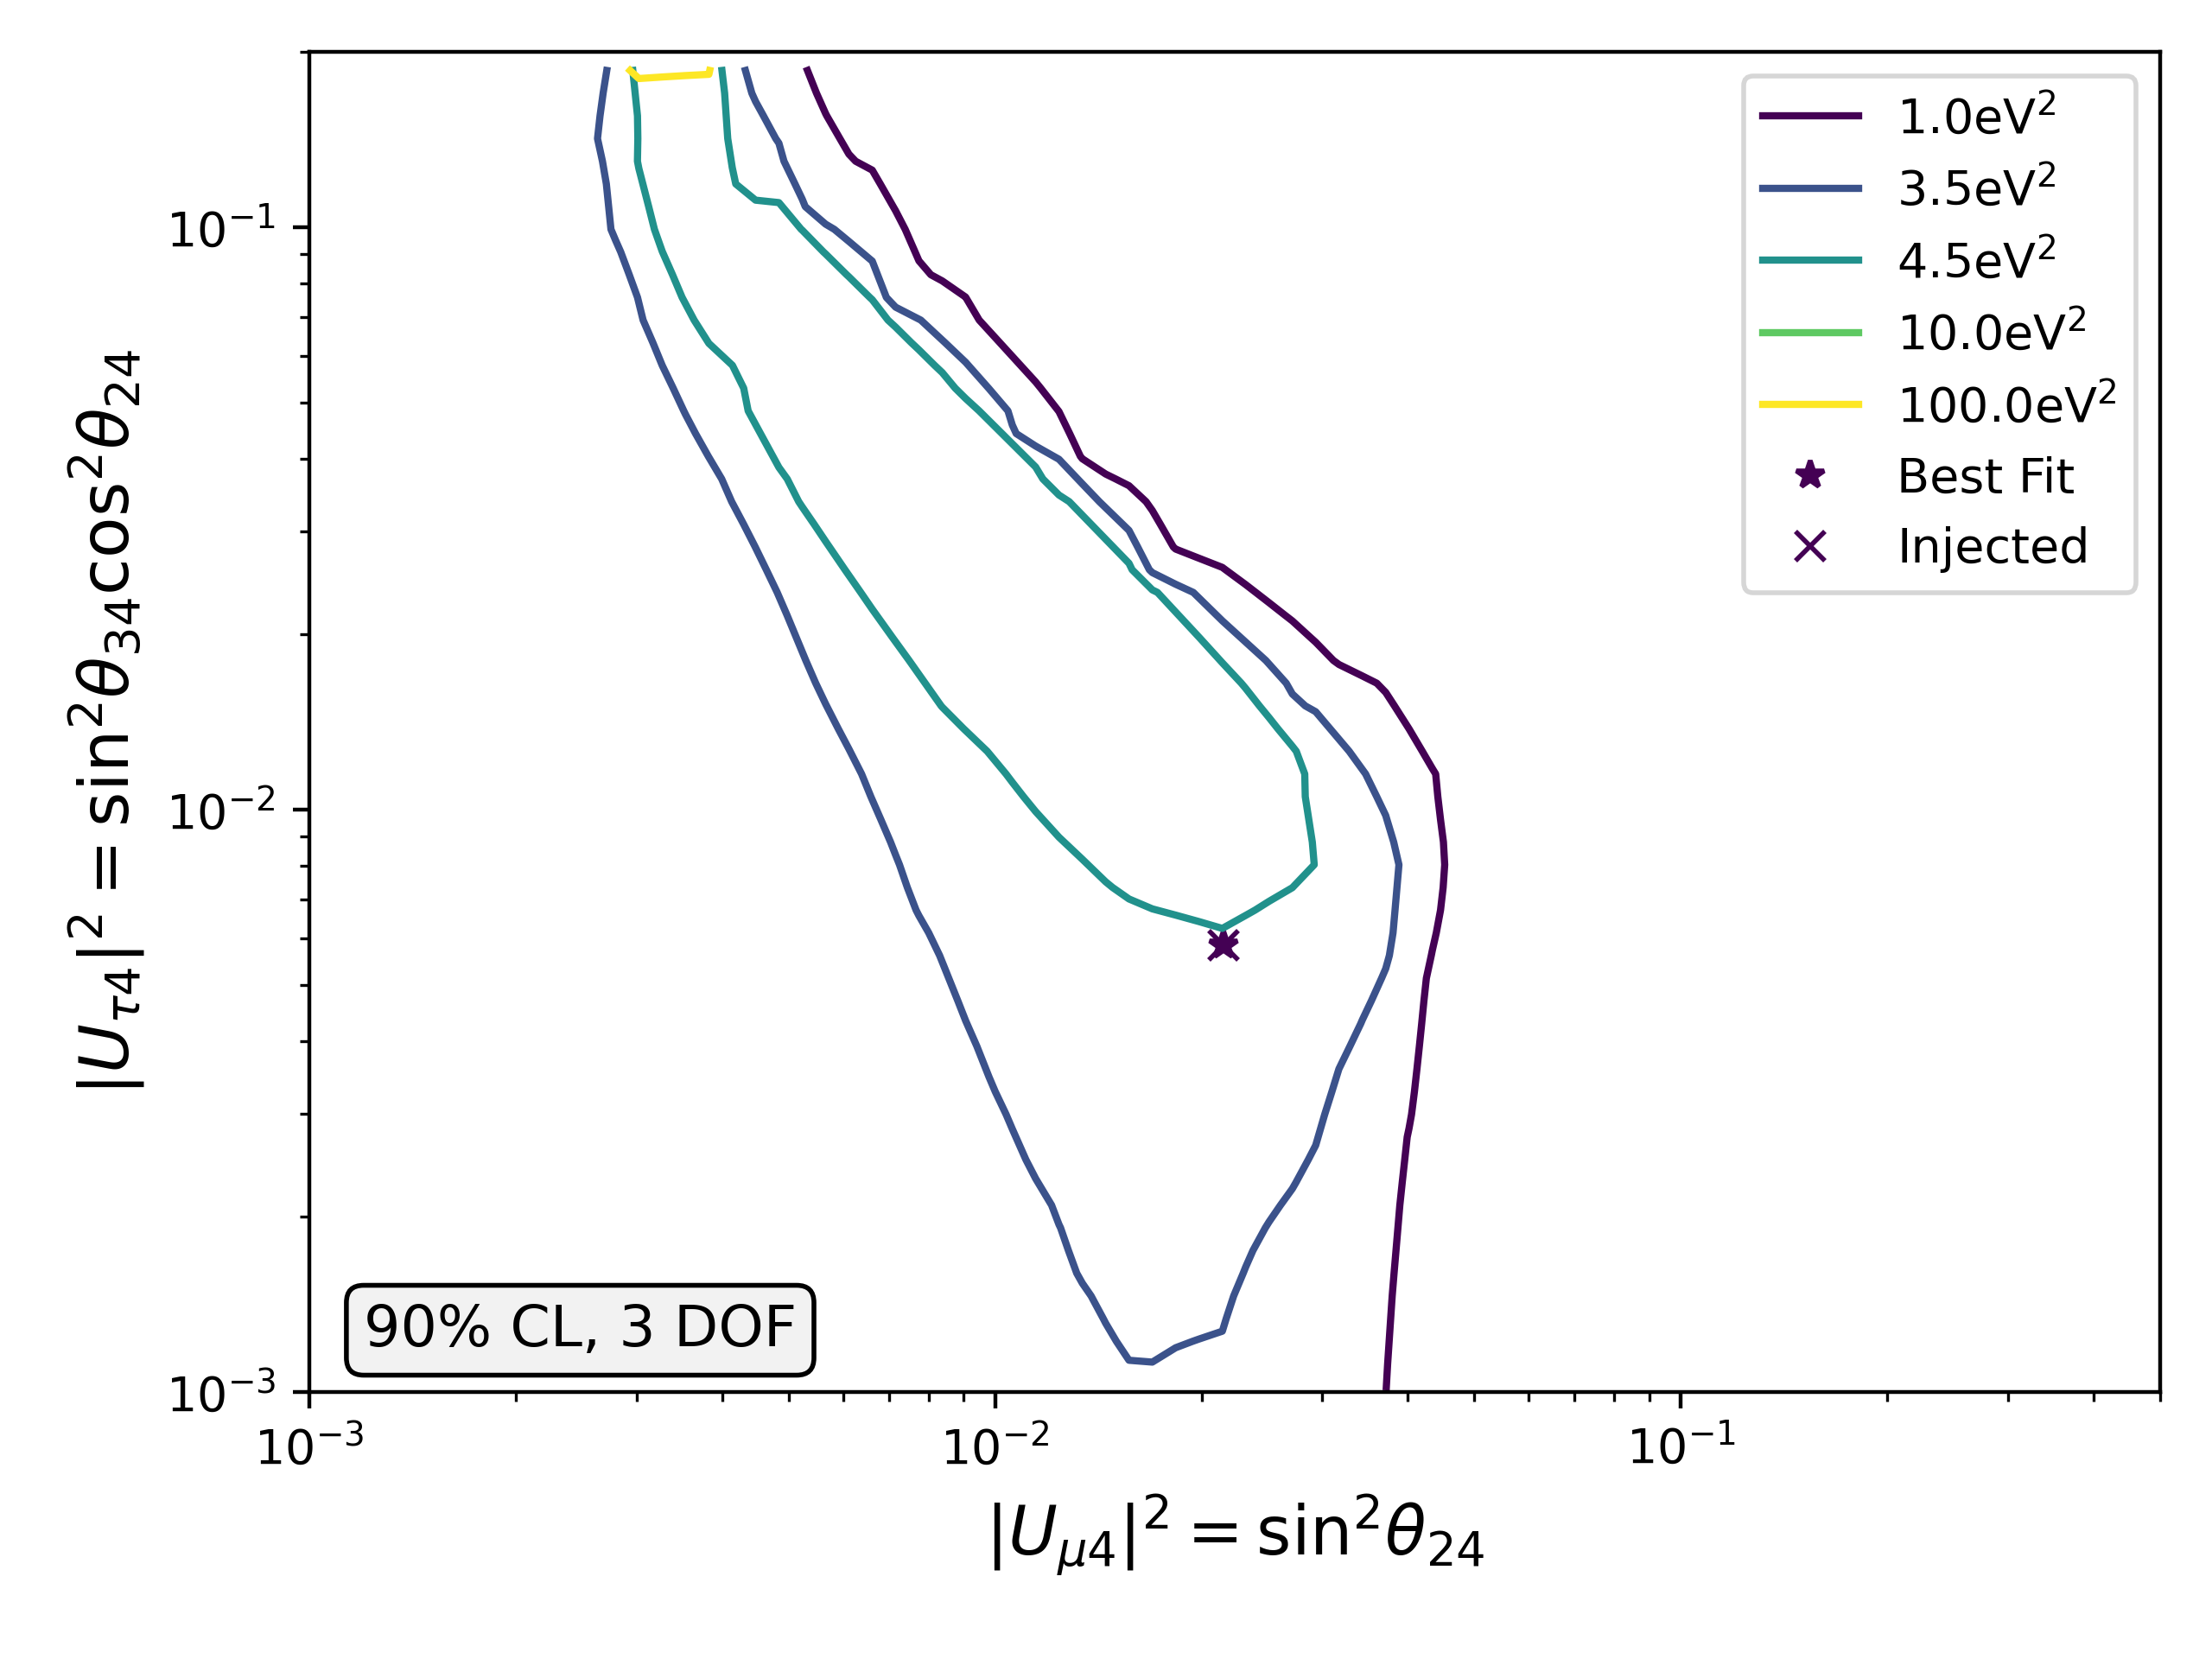
\includegraphics[width=0.45\linewidth]{figures/inject_recover_RealIR_1_sterile_1_cl0.9_dof3.png}
    \caption{Two signal inject-recover tests.}\label{fig:first_ir}
\end{figure}

\begin{figure}
    \centering
    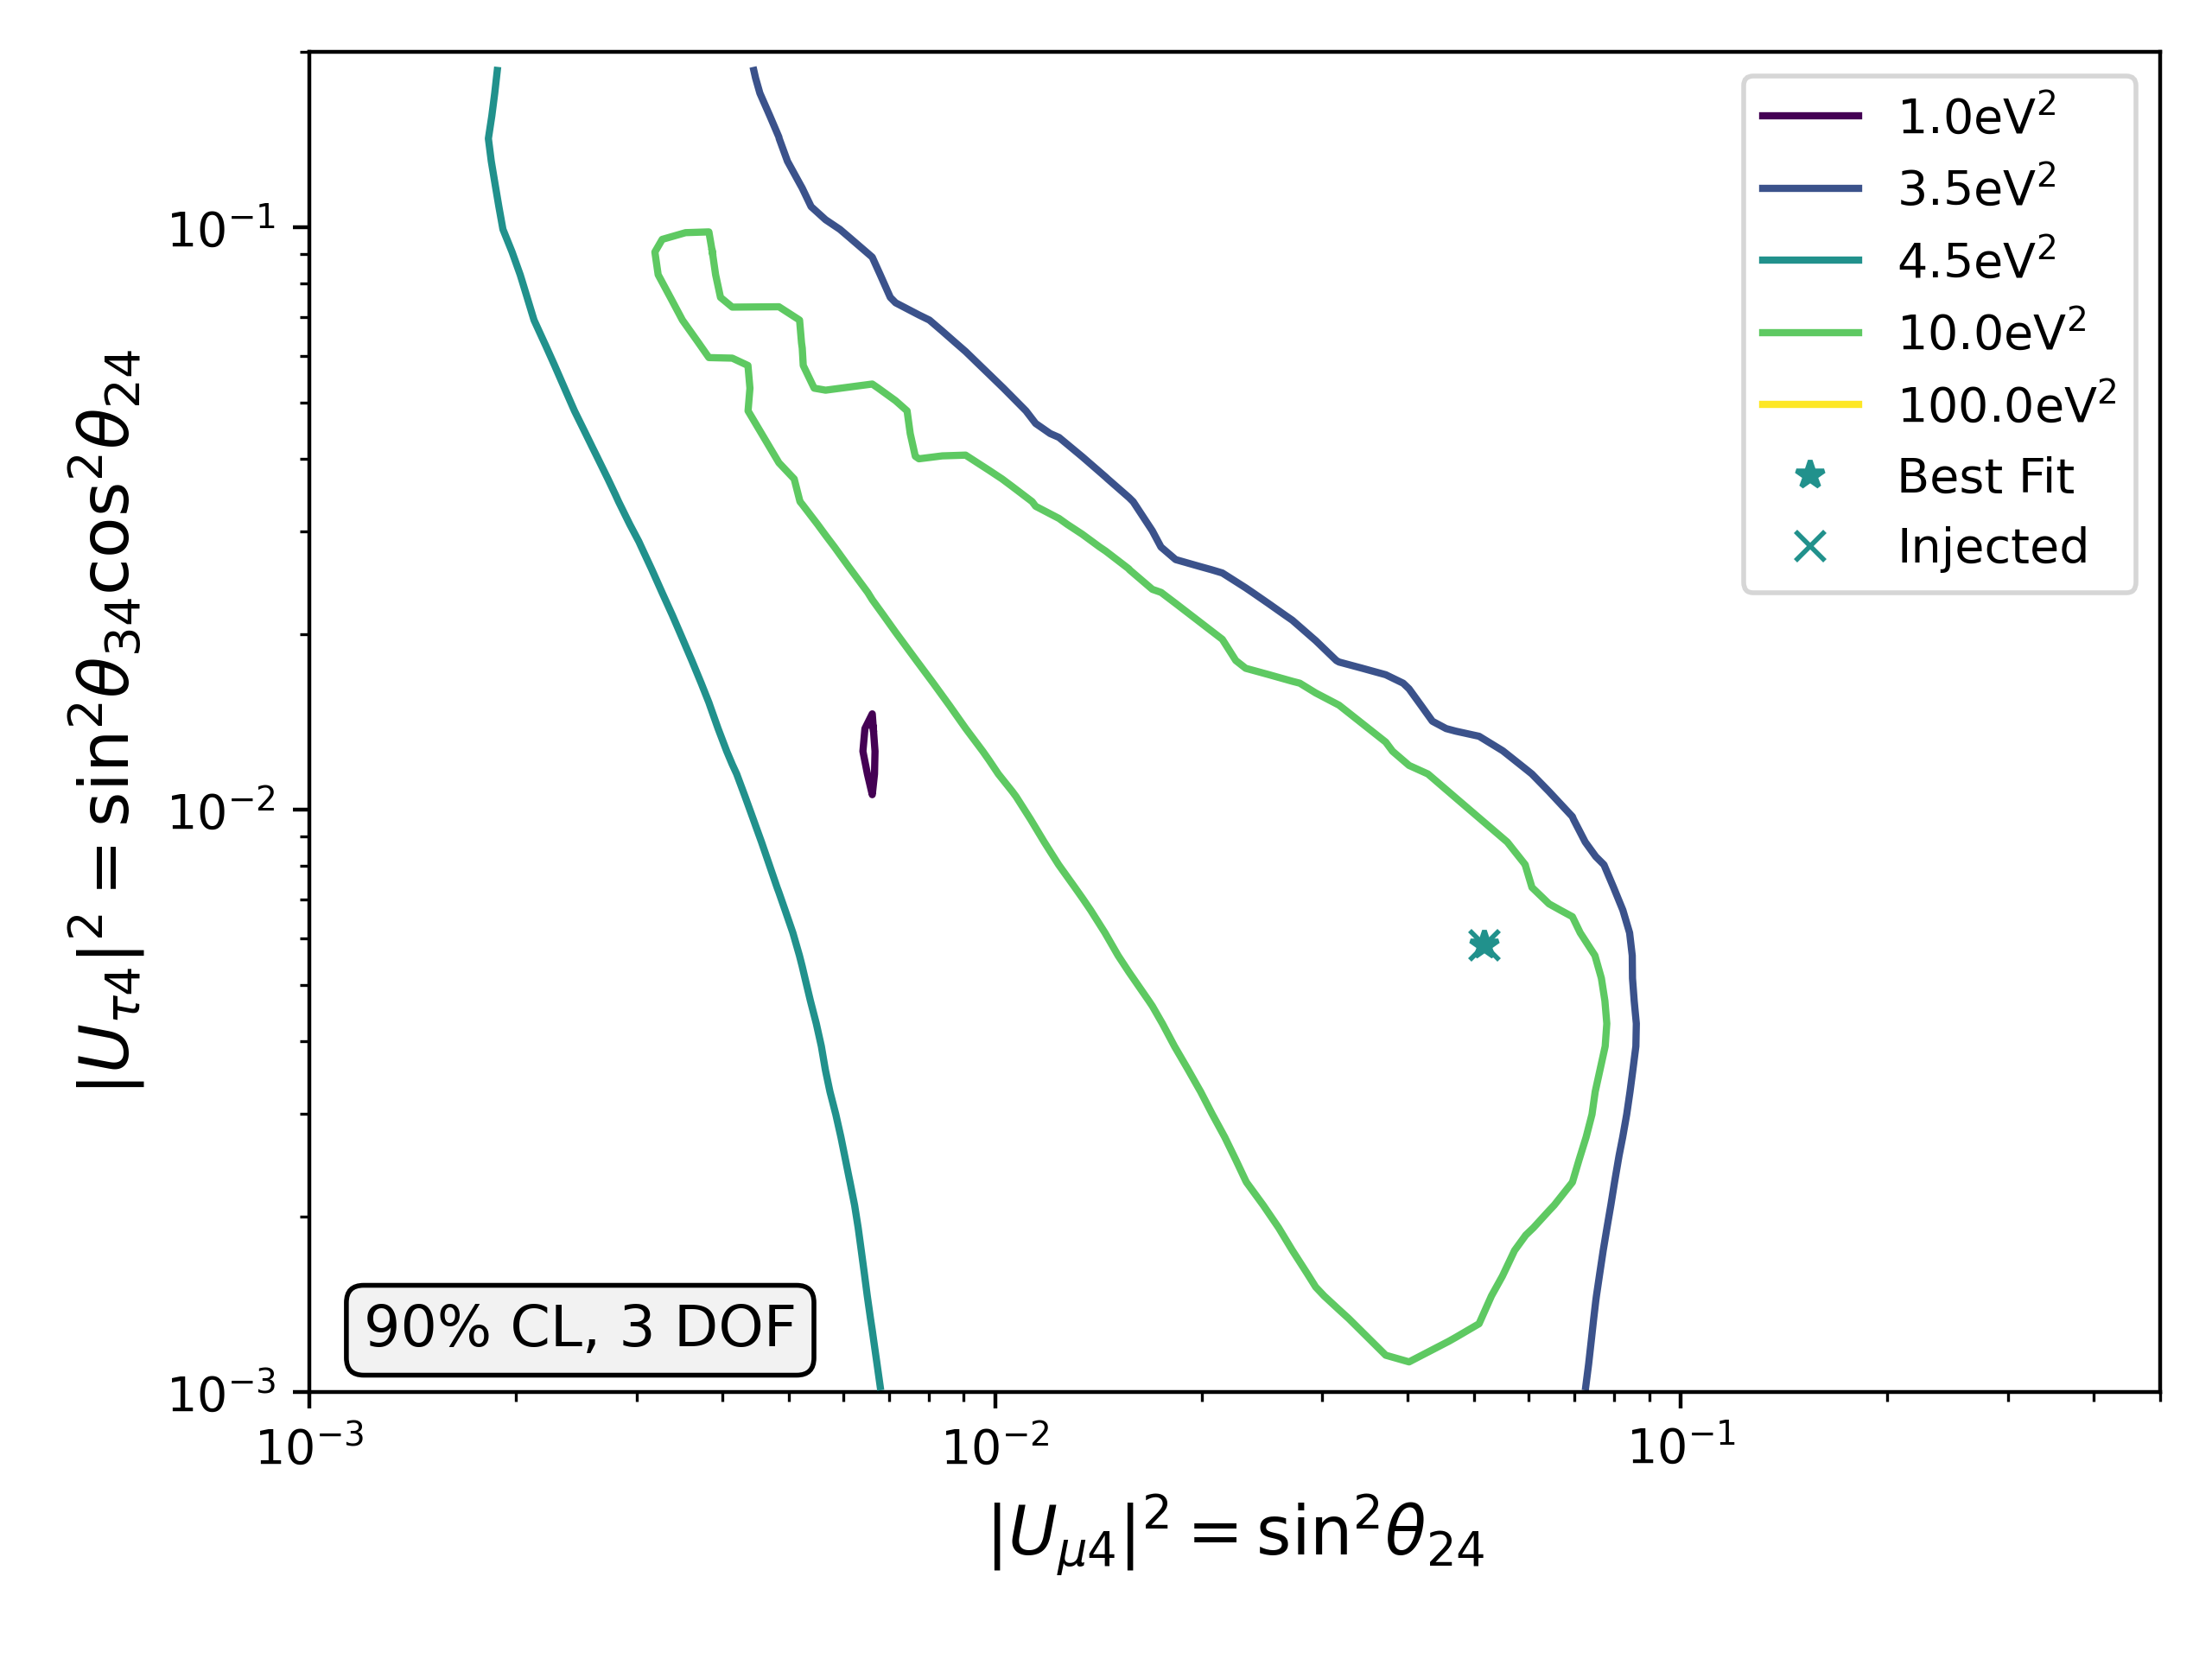
\includegraphics[width=0.45\linewidth]{figures/inject_recover_RealIR_2_sterile_4_cl0.9_dof3.png}%
    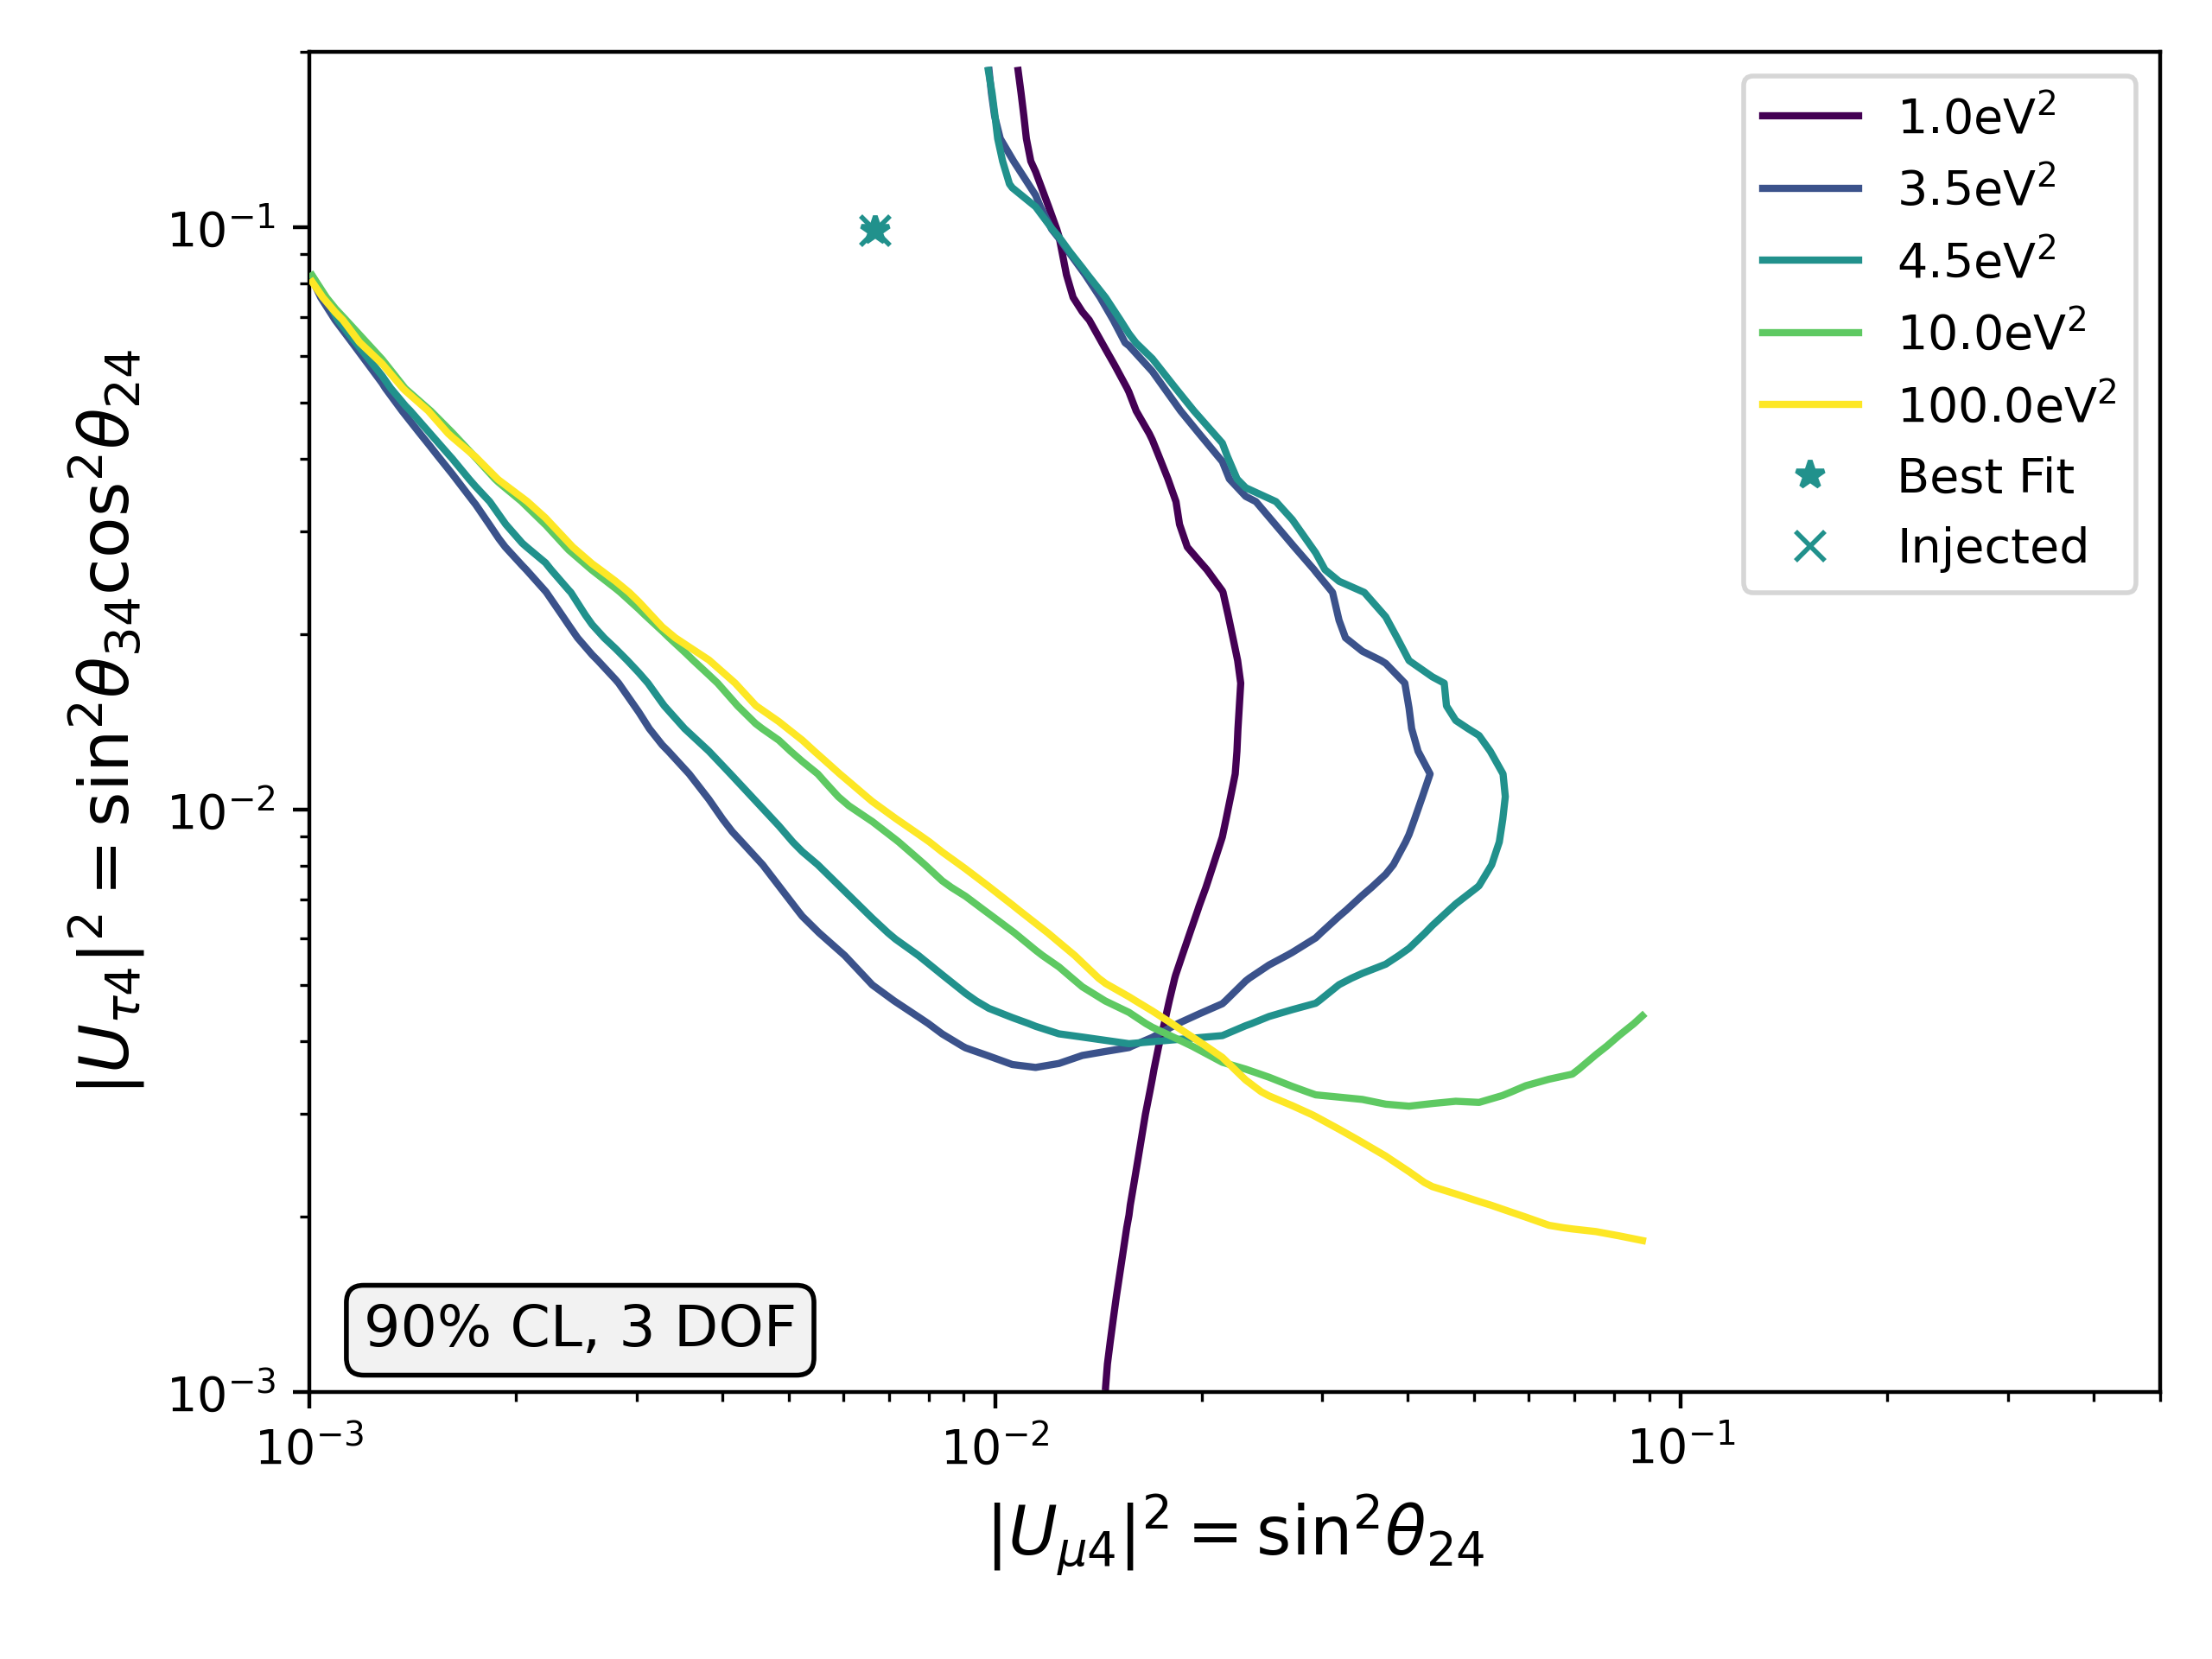
\includegraphics[width=0.45\linewidth]{figures/inject_recover_RealIR_3_sterile_4_cl0.9_dof3.png}
    \caption{Two signal inject-recover tests.}
\end{figure}


\begin{figure}
    \centering
    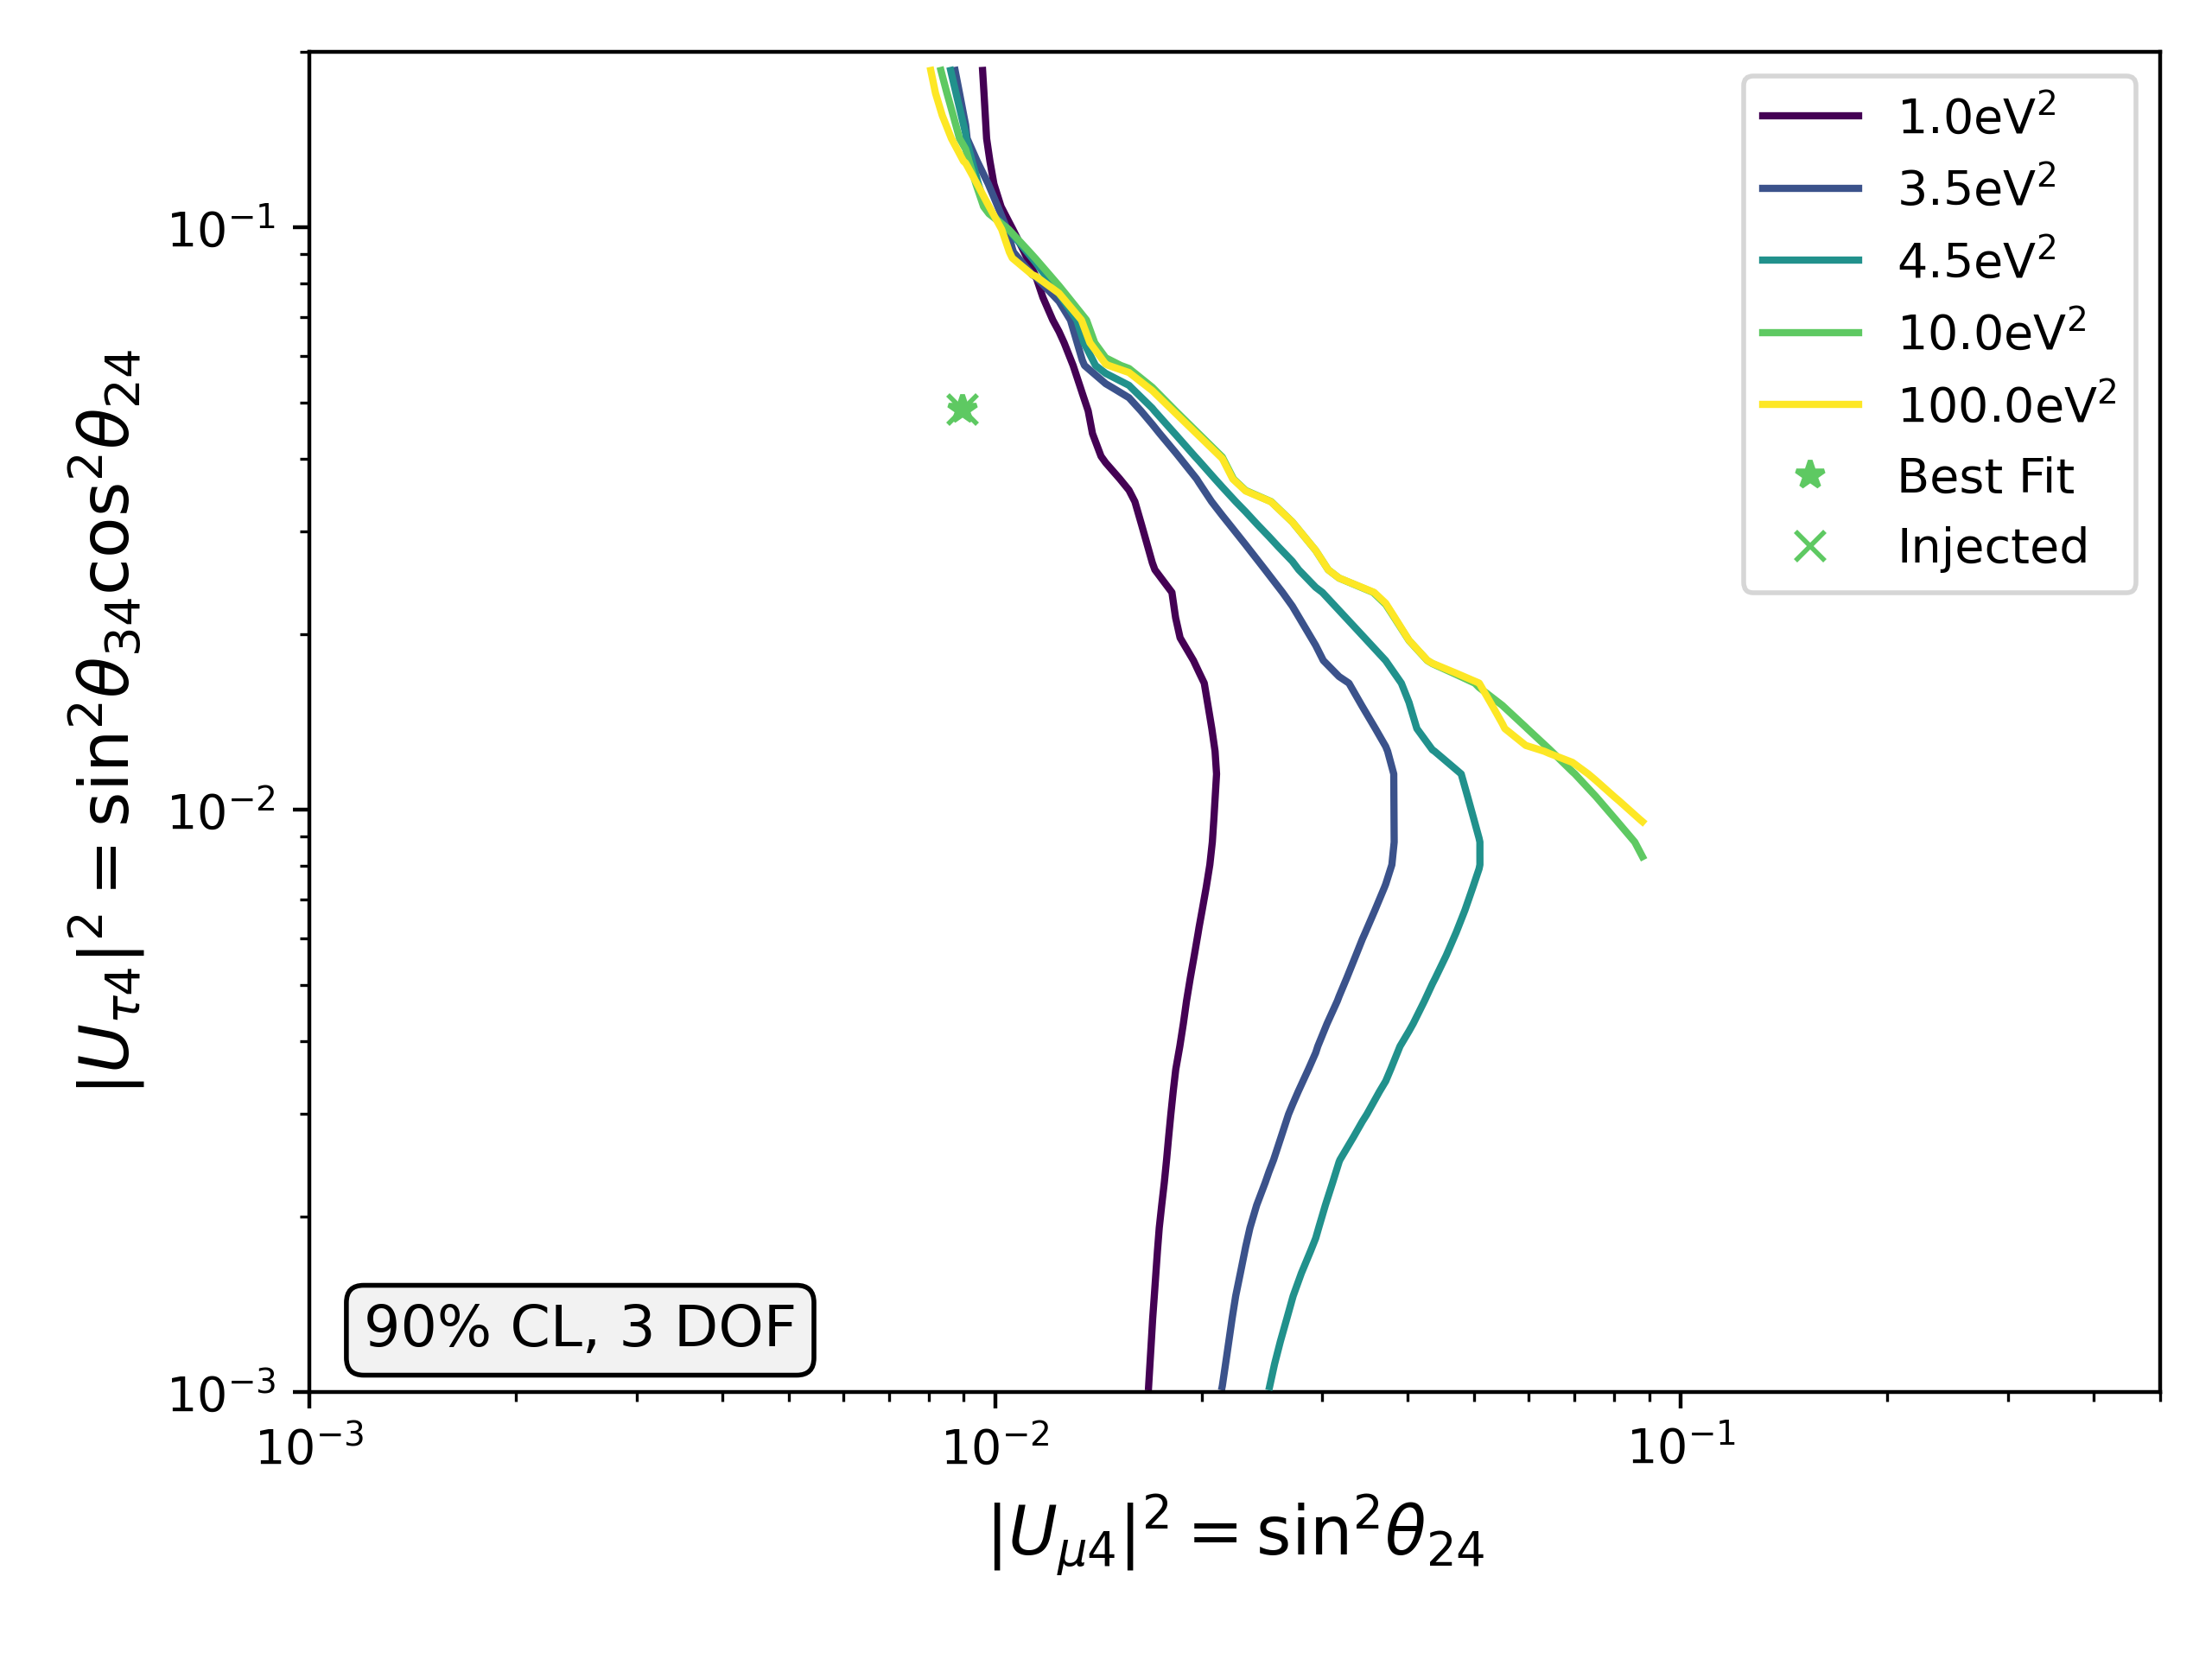
\includegraphics[width=0.45\linewidth]{figures/inject_recover_RealIR_5_sterile_1_cl0.9_dof3.png}%
    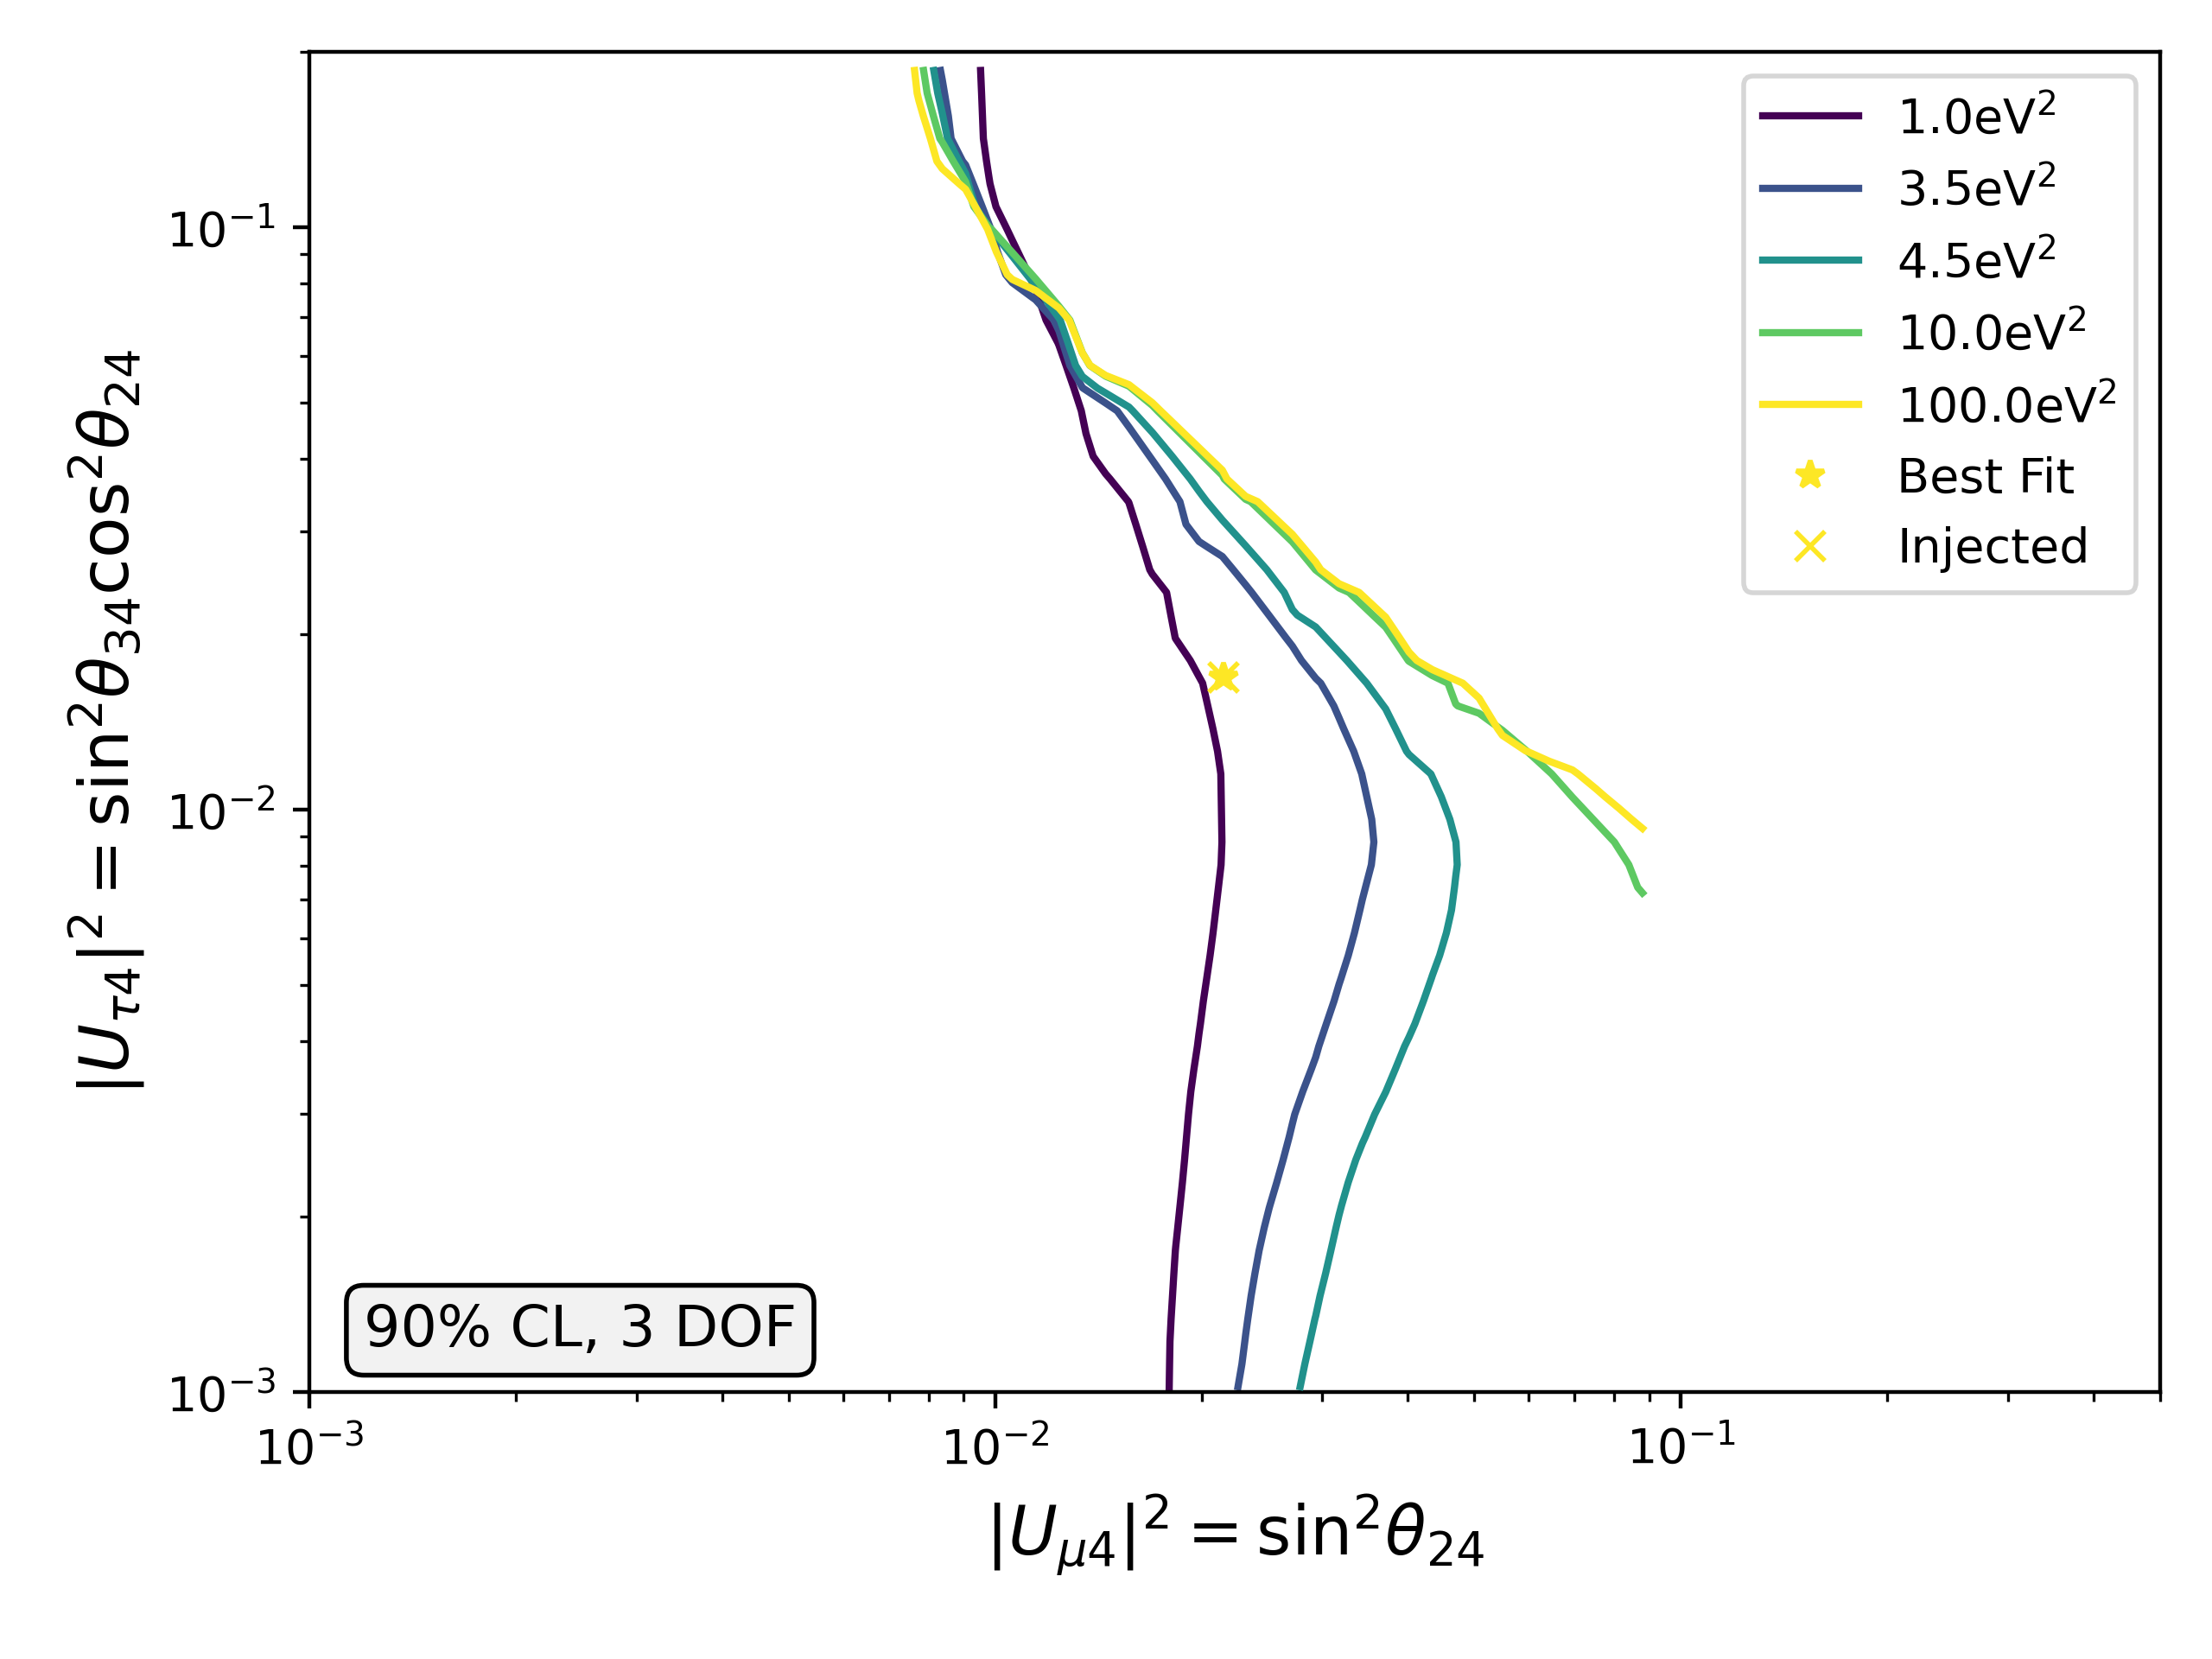
\includegraphics[width=0.45\linewidth]{figures/inject_recover_RealIR_6_sterile_1_cl0.9_dof3.png}
    \caption{Two signal inject-recover tests.}
\end{figure}

\begin{figure}
    \centering
    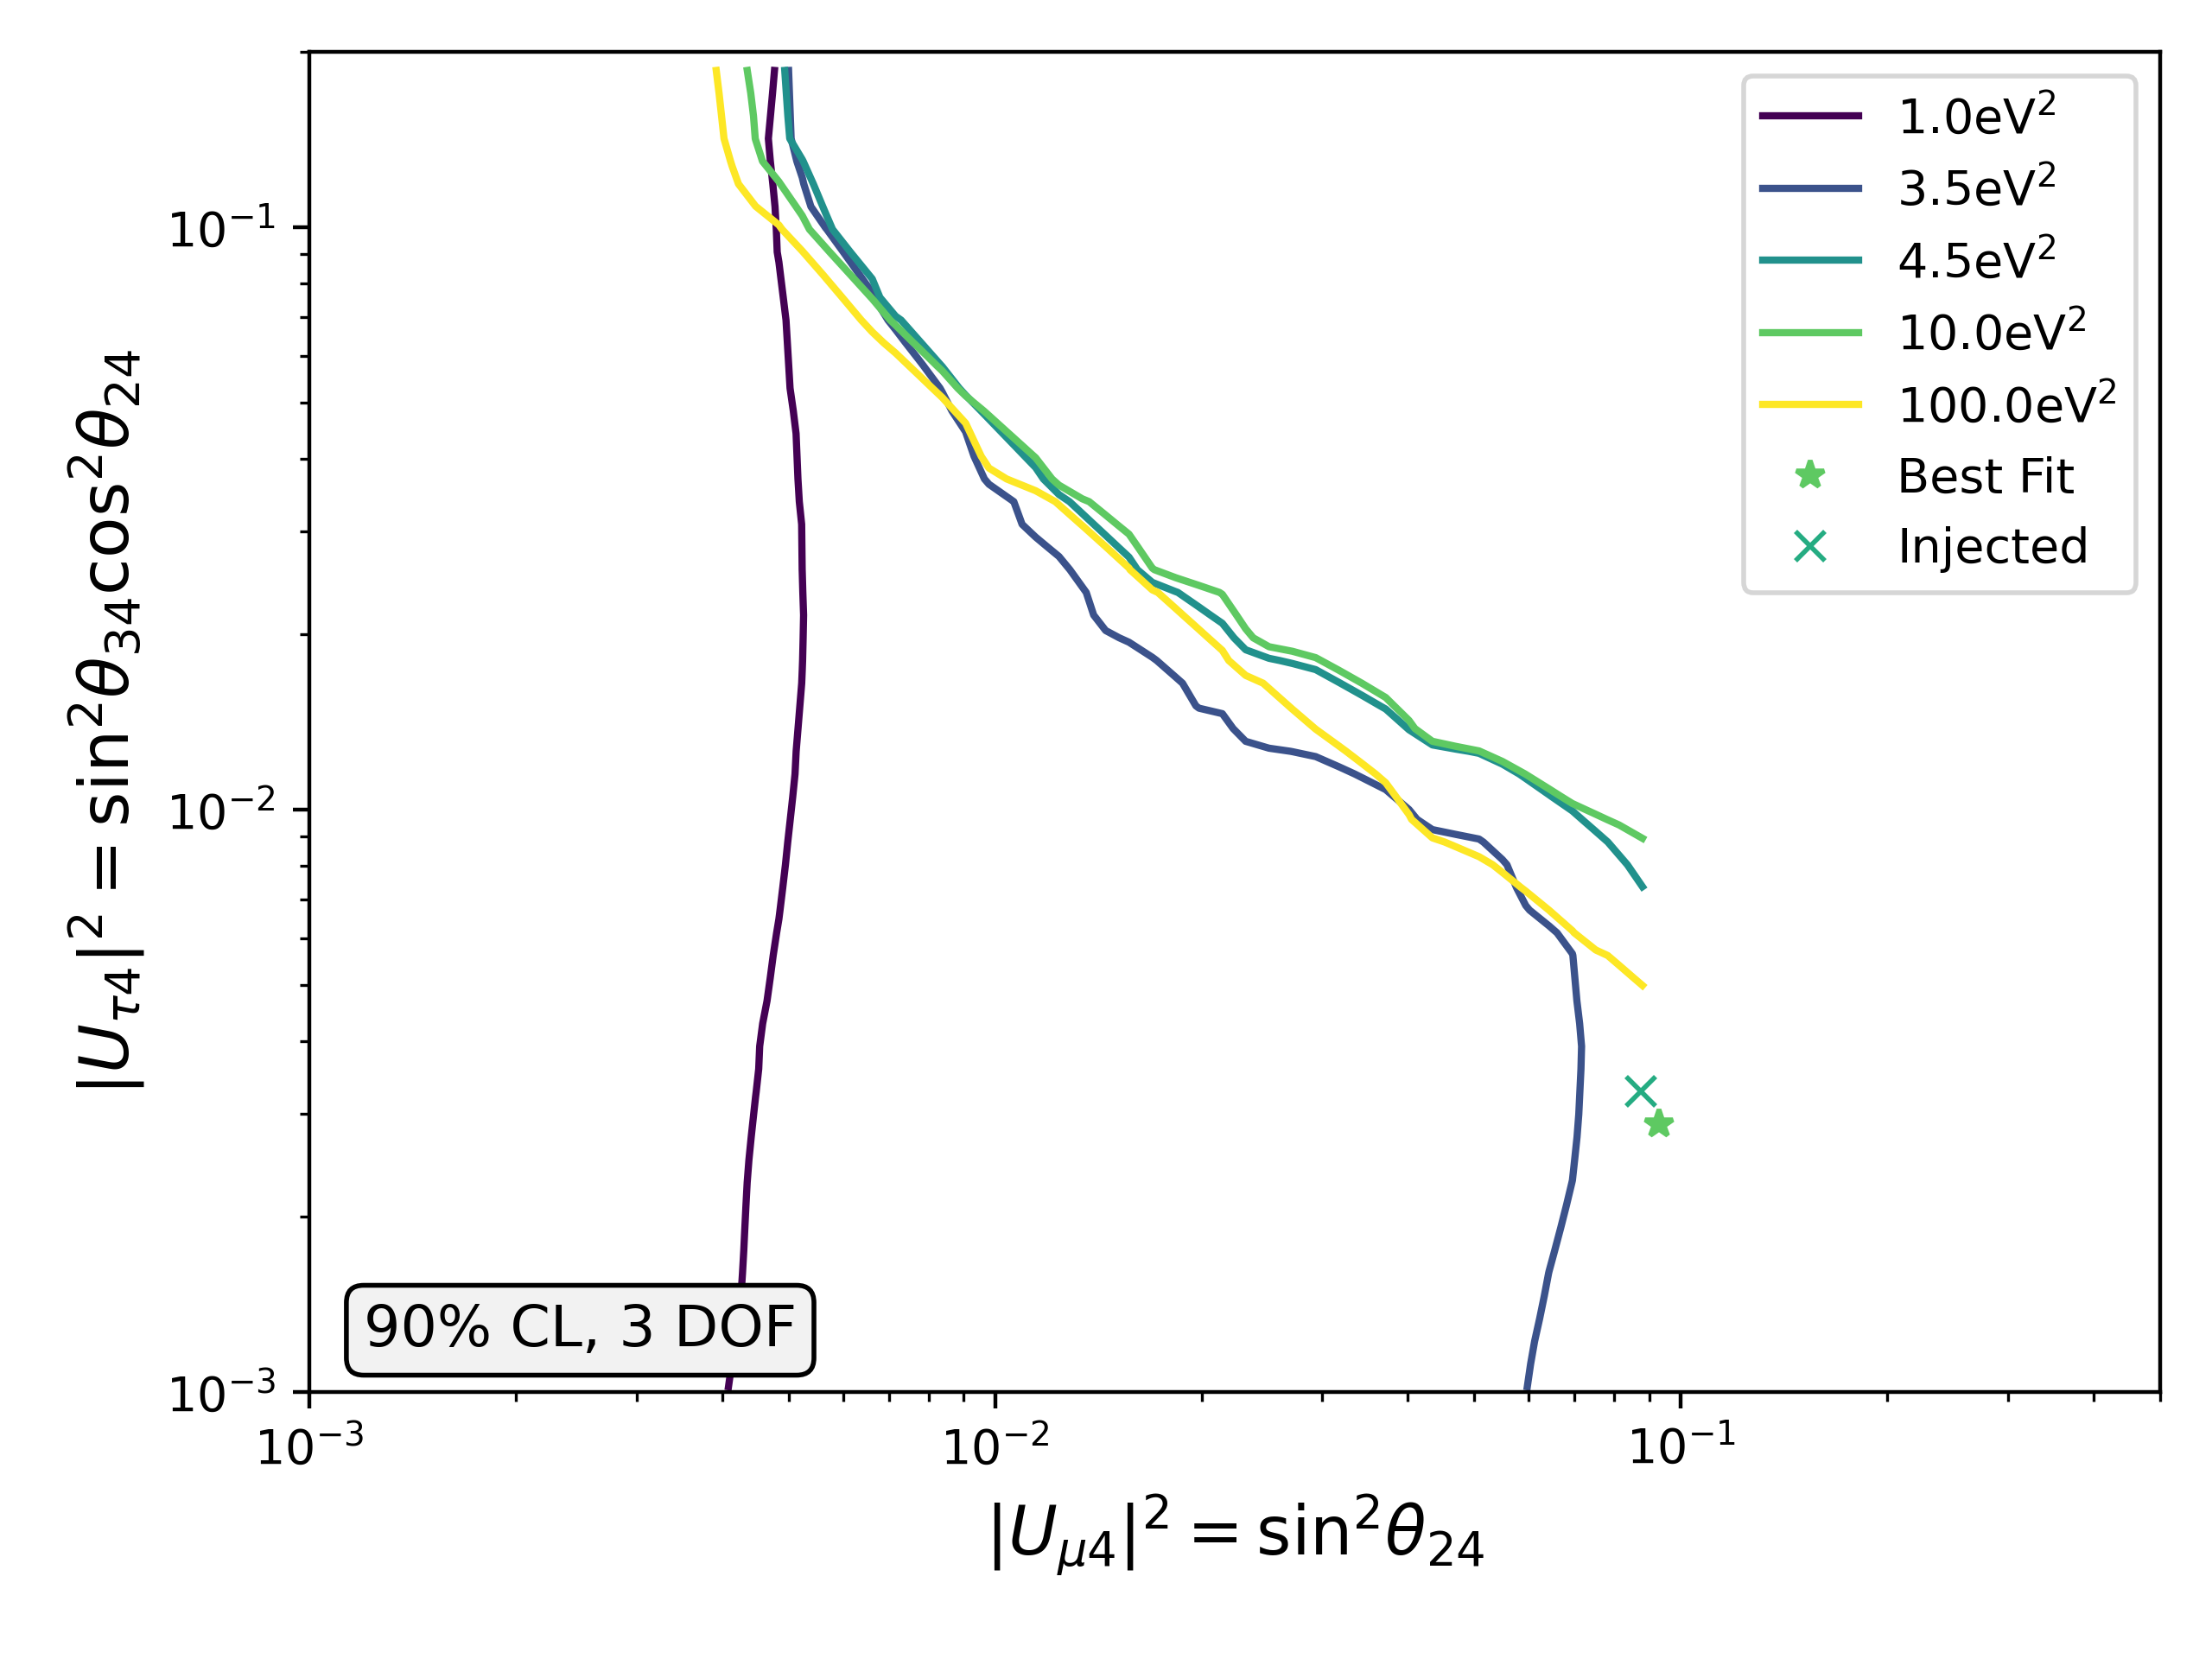
\includegraphics[width=0.45\linewidth]{figures/inject_recover_RealIR_8_sterile_7_cl0.9_dof3.png}%
    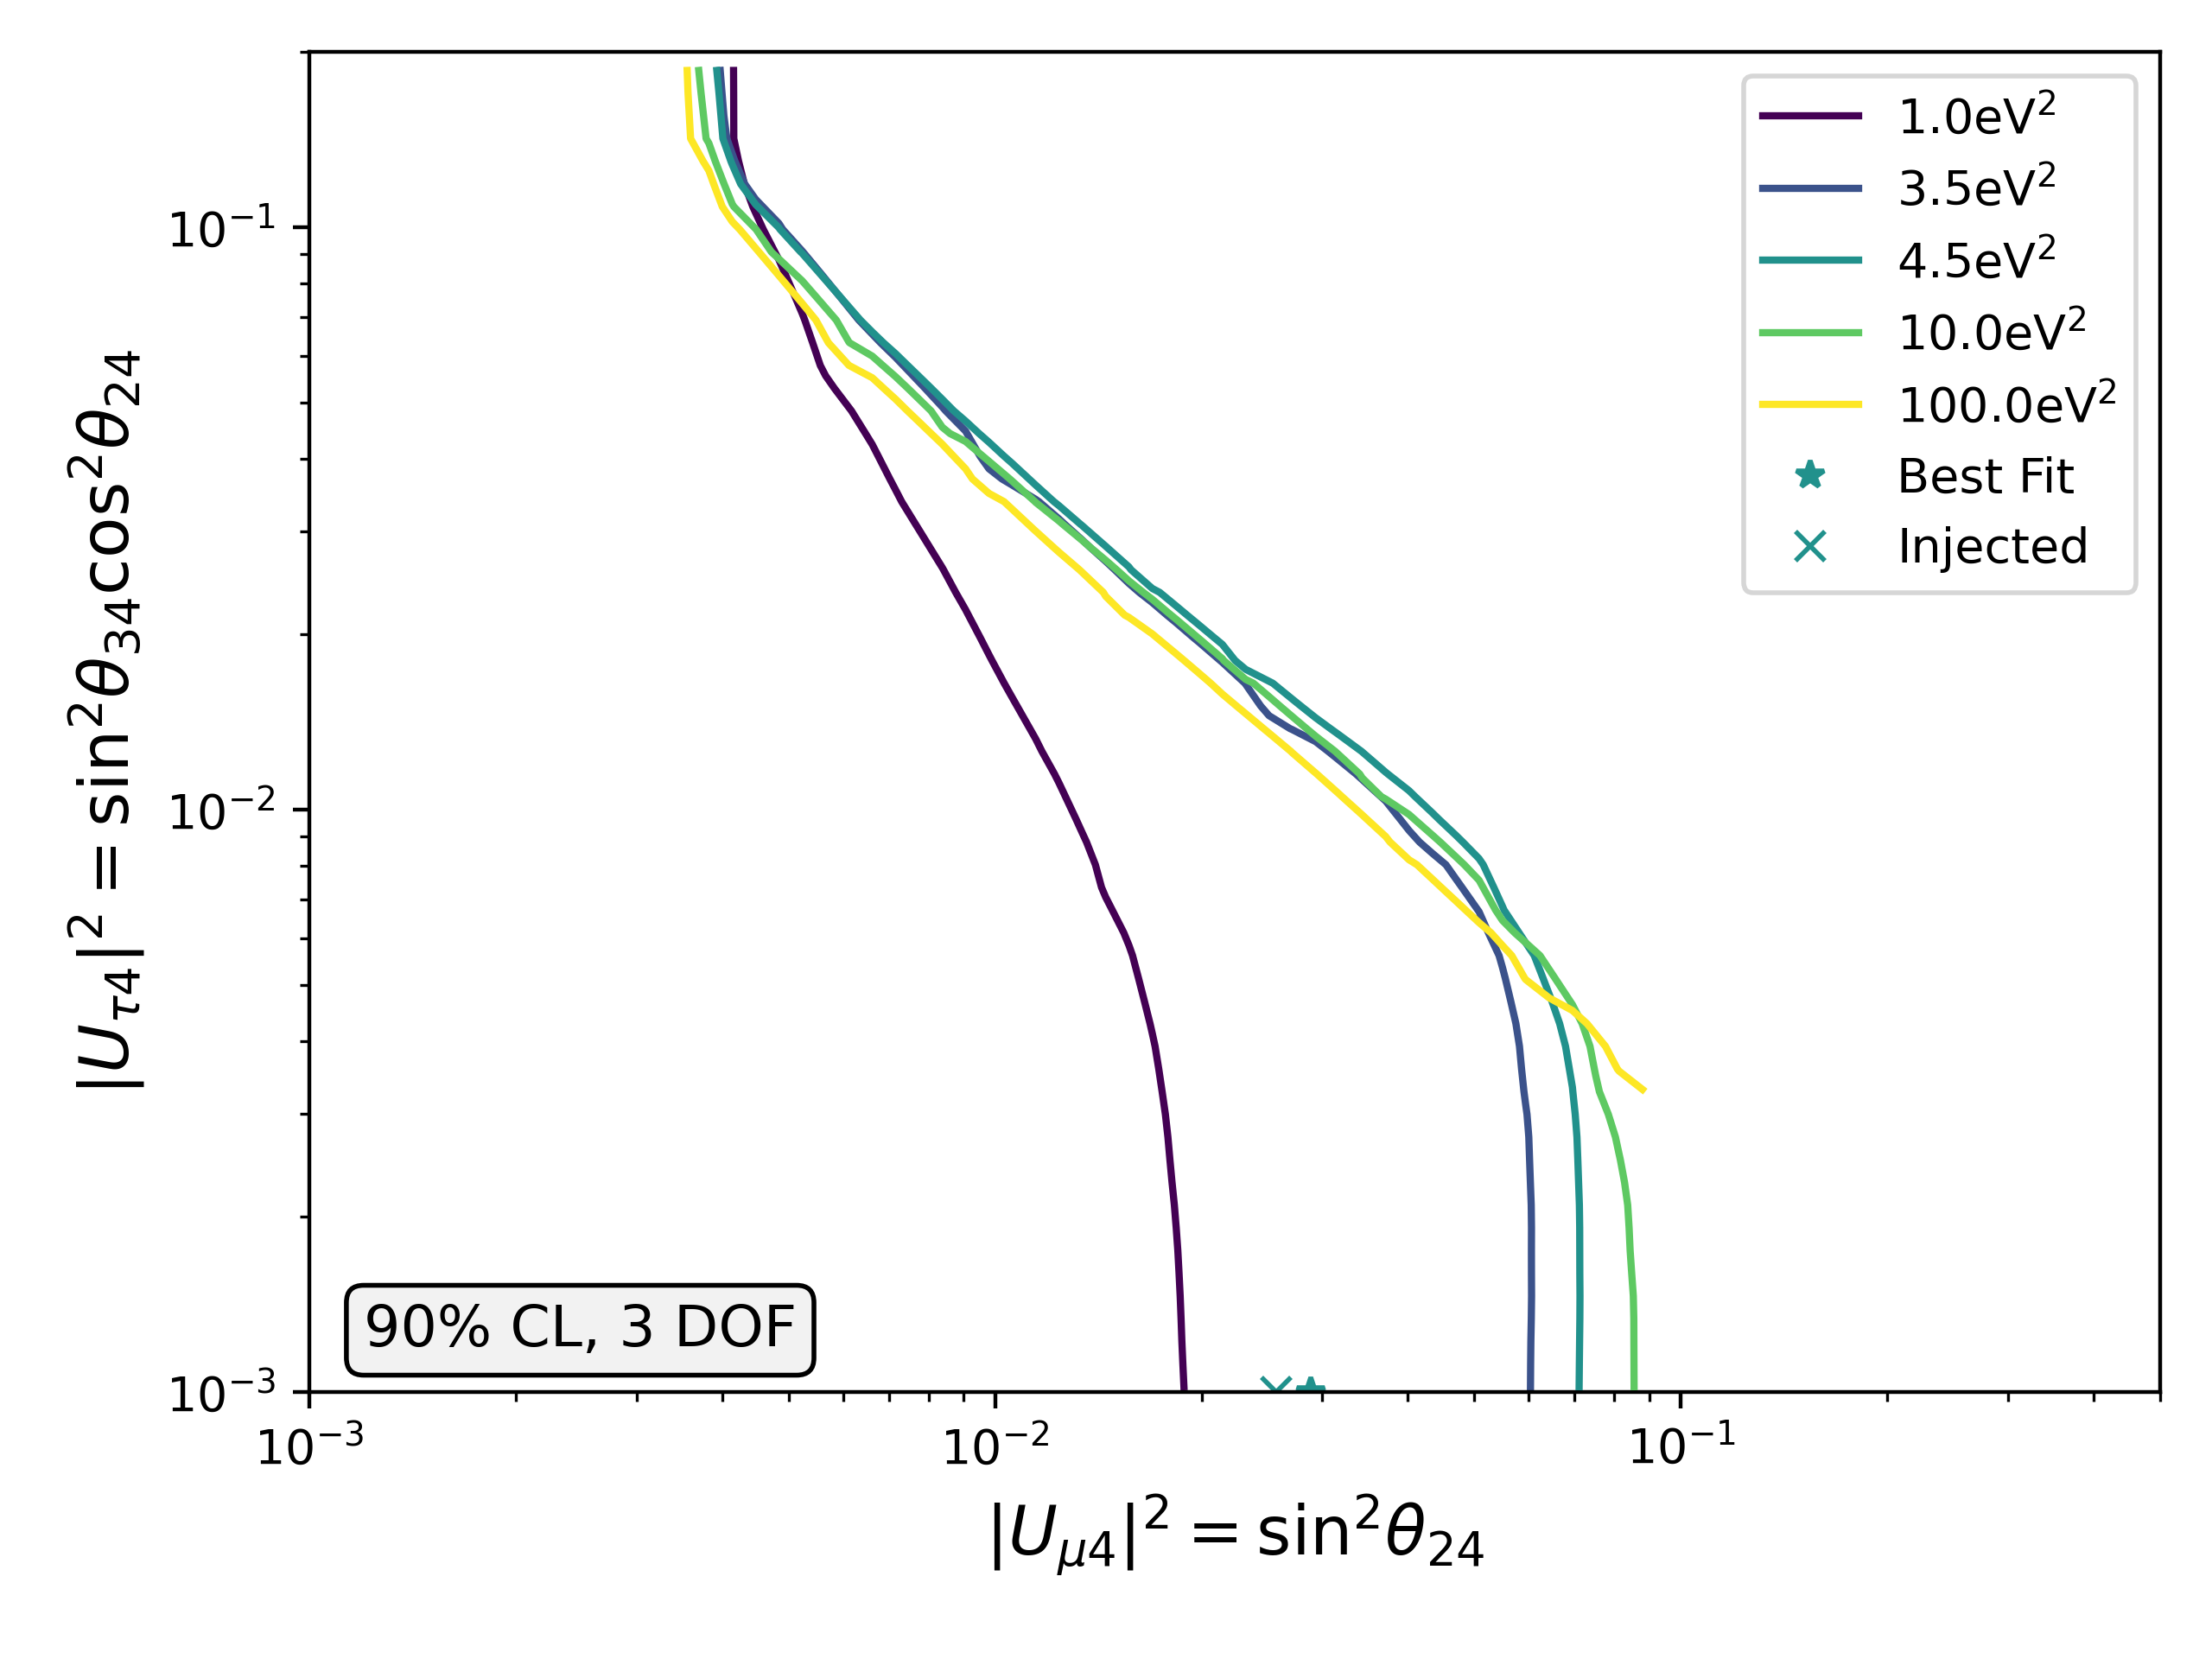
\includegraphics[width=0.45\linewidth]{figures/inject_recover_RealIR_9_sterile_4_cl0.9_dof3.png}
    \caption{Two signal inject-recover tests.}\label{fig:last_ir}
\end{figure}

\section{Sensitivities}

\subsection{Asimov Sensitivity}

Two Asimov fit-scans were carried out: once using the conventional flux model from the 8-year analysis and one using daemonflux. 
The 90\% confidence level $\chi^{2}$ threshold was calculated for three degrees of freedom for each fit scan, and the resulting sensitivity contours are shown in Figure~\ref{fig:asimov_daemon_sense} using daemonflux. 
Sensitivities for the two different models are shown, overlain, in Figure~\ref{fig:asimov_model_compare}; here the astrophysical flavor ratio uncertainty was not included in either scan. 
The change in sensitivity where daemonflux is used as the nominal conventional flux model is due to the difference in the predicted charge ratio; daemonflux predicts a higher charge ratio and therefore a smaller signature from the resonant $\bar{\nu_{\mu}}$ disappearance. 

These results are plotted compared to the previous phenomenological predictions in Figure~\ref{fig:pheno_compare}. 
Sensitivities are compared at 90\% confidence level and assuming two degrees of freedom $\Delta m_{41}^{2}=$ 1.0 eV$^{2}$.
The sensitivities calculated for this analysis are similar, although somewhat worse than those predicted earlier in Chapter~\ref{chapter:sense}. This is not surprising; here a full treatment of systematic uncertainty is used. 
We also compare the two degrees of freedom sensitivity at 1.0 eV$^{2}$ for this analysis to the results of Super-Kamiokande~\cite{PhysRevD.91.052019} and DeepCore~\cite{Aartsen_2017_dc} in Figure~\ref{fig:experiment_compare}.
We find that this analysis has strong sensitivity to $\abs{U_{\mu 4}}^{2}$ when compared to other existing constraints. 

\begin{figure}
    \centering
    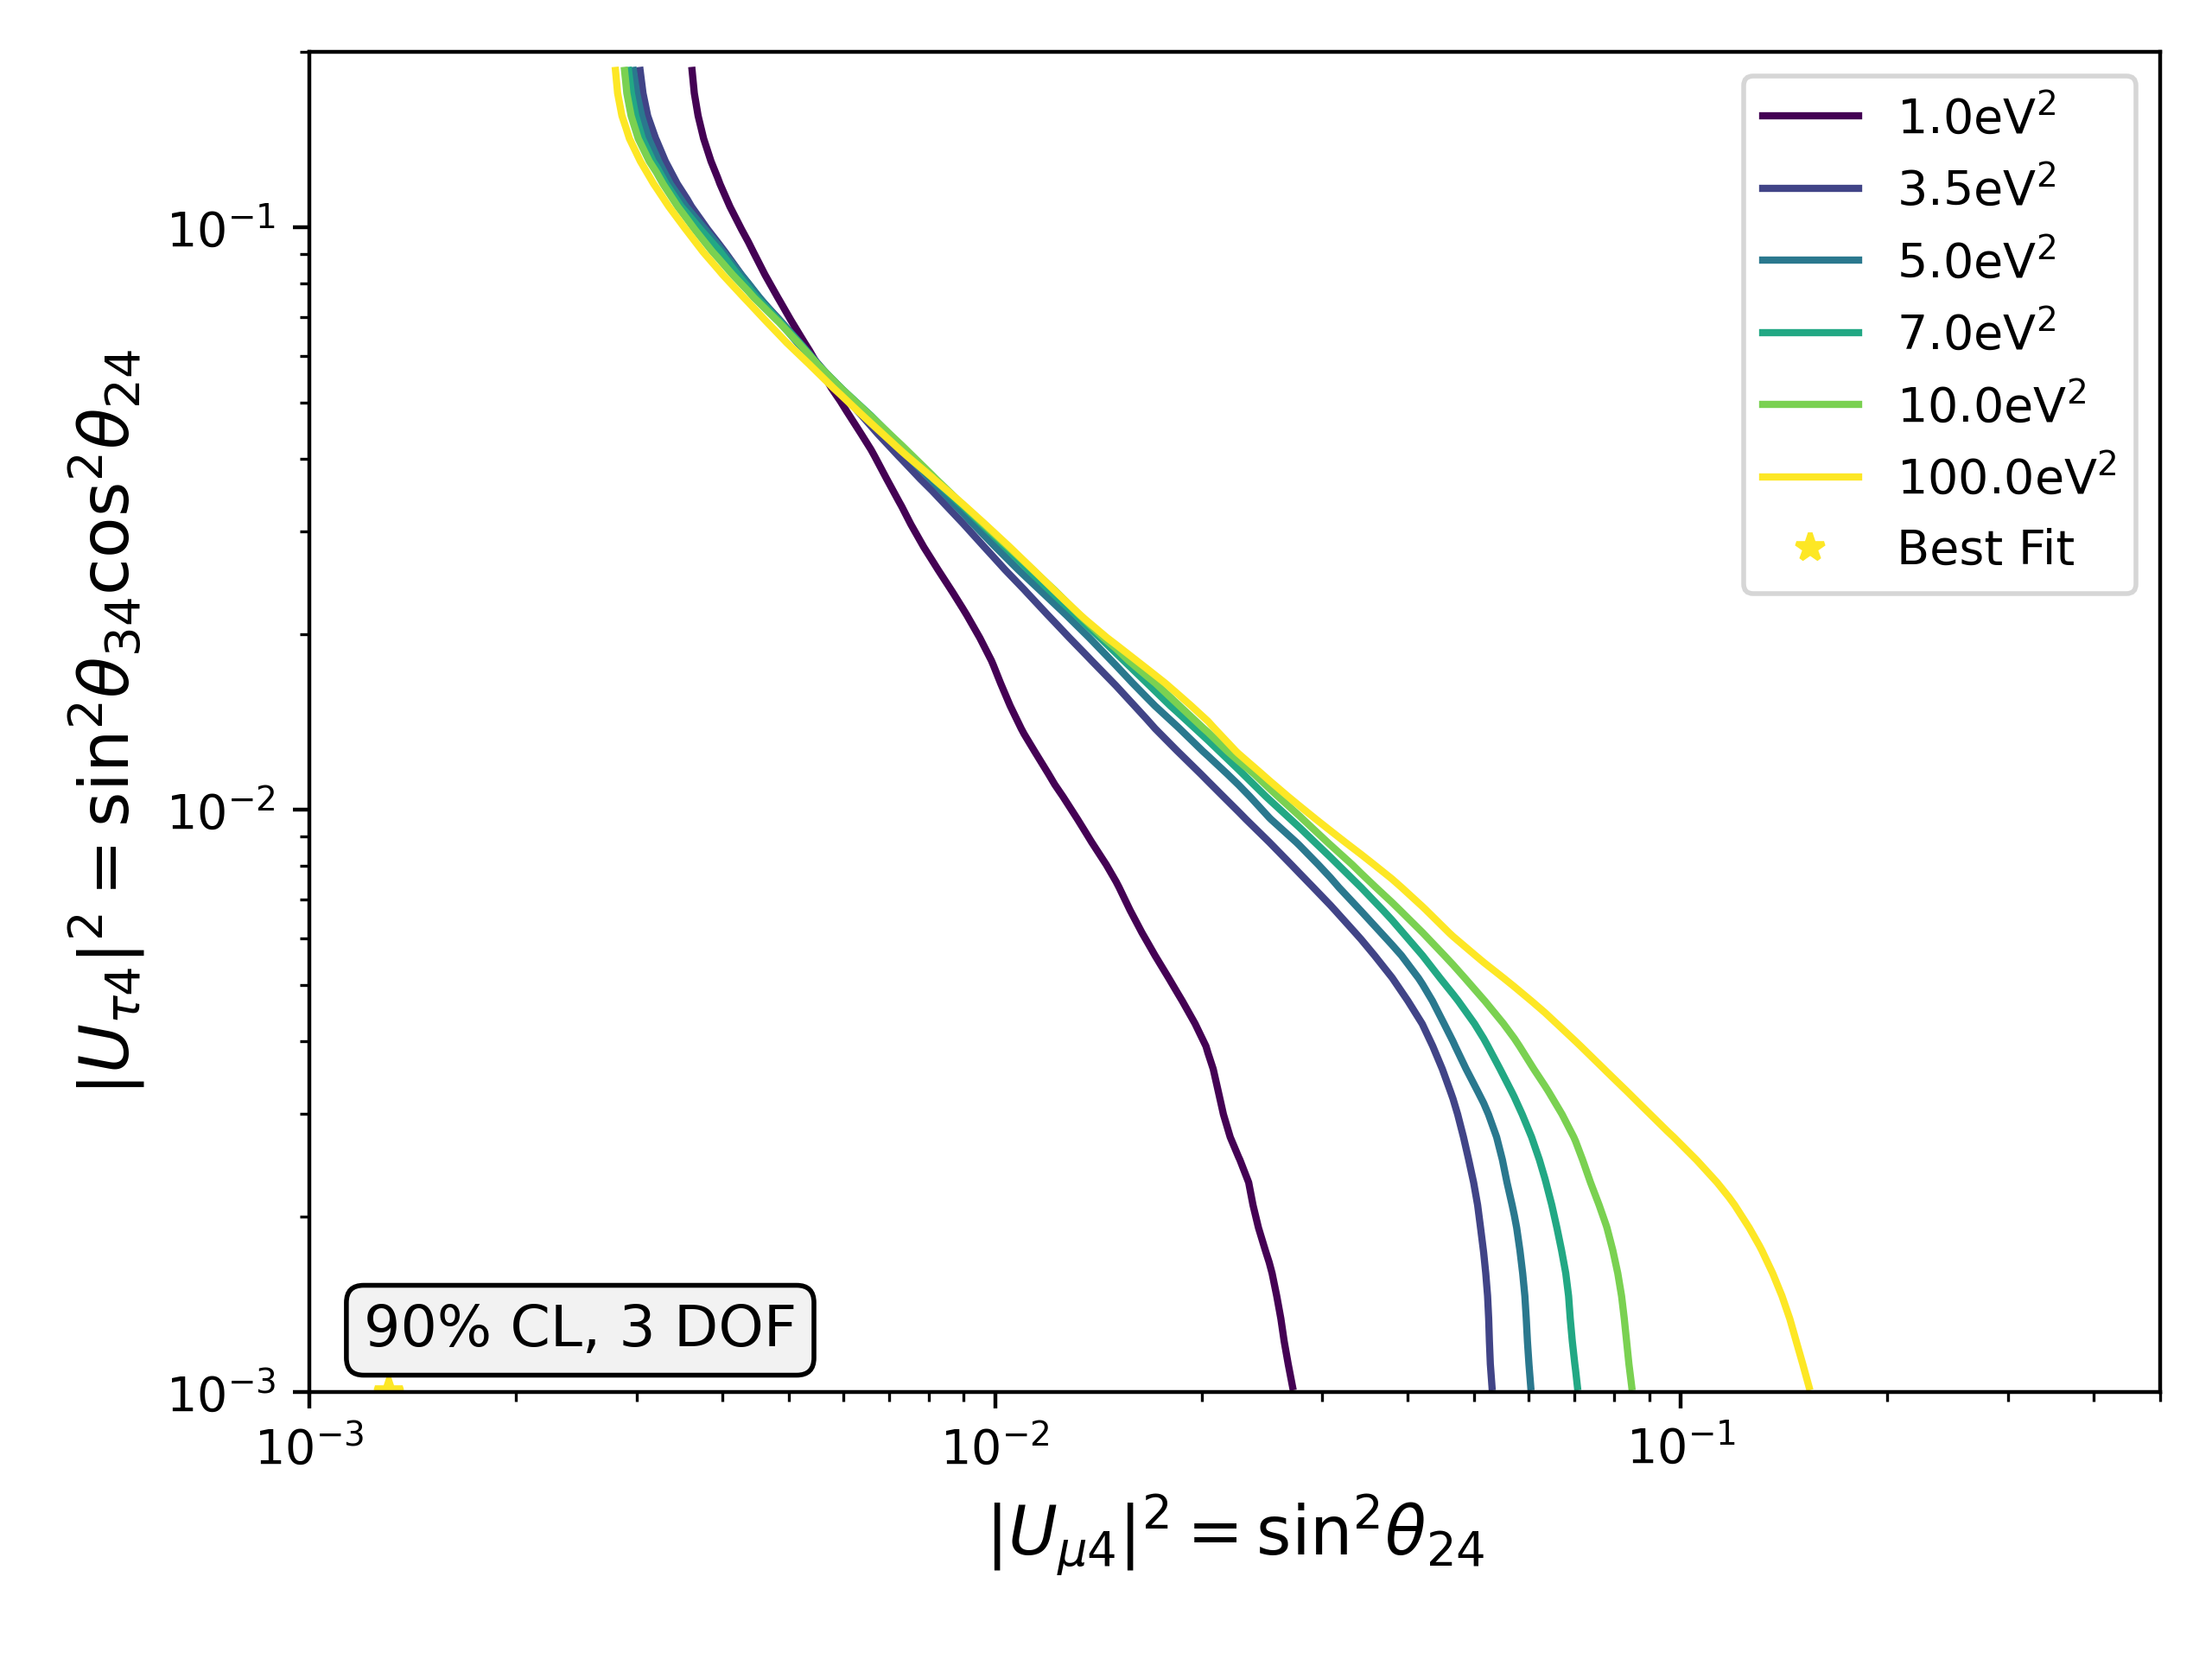
\includegraphics[width=0.7\linewidth]{figures/joint_daemon_asimov_with_flavor_update_Realization_daemon_newflavor_Asimov_sterile_0_cl0.9_dof3.png}
    \caption{The 90\% confidence level sensitivity contours with three degrees of freedom for this analysis; using daemonflux for the conventional flux model}\label{fig:asimov_daemon_sense}
\end{figure}

\begin{figure}
    \centering
    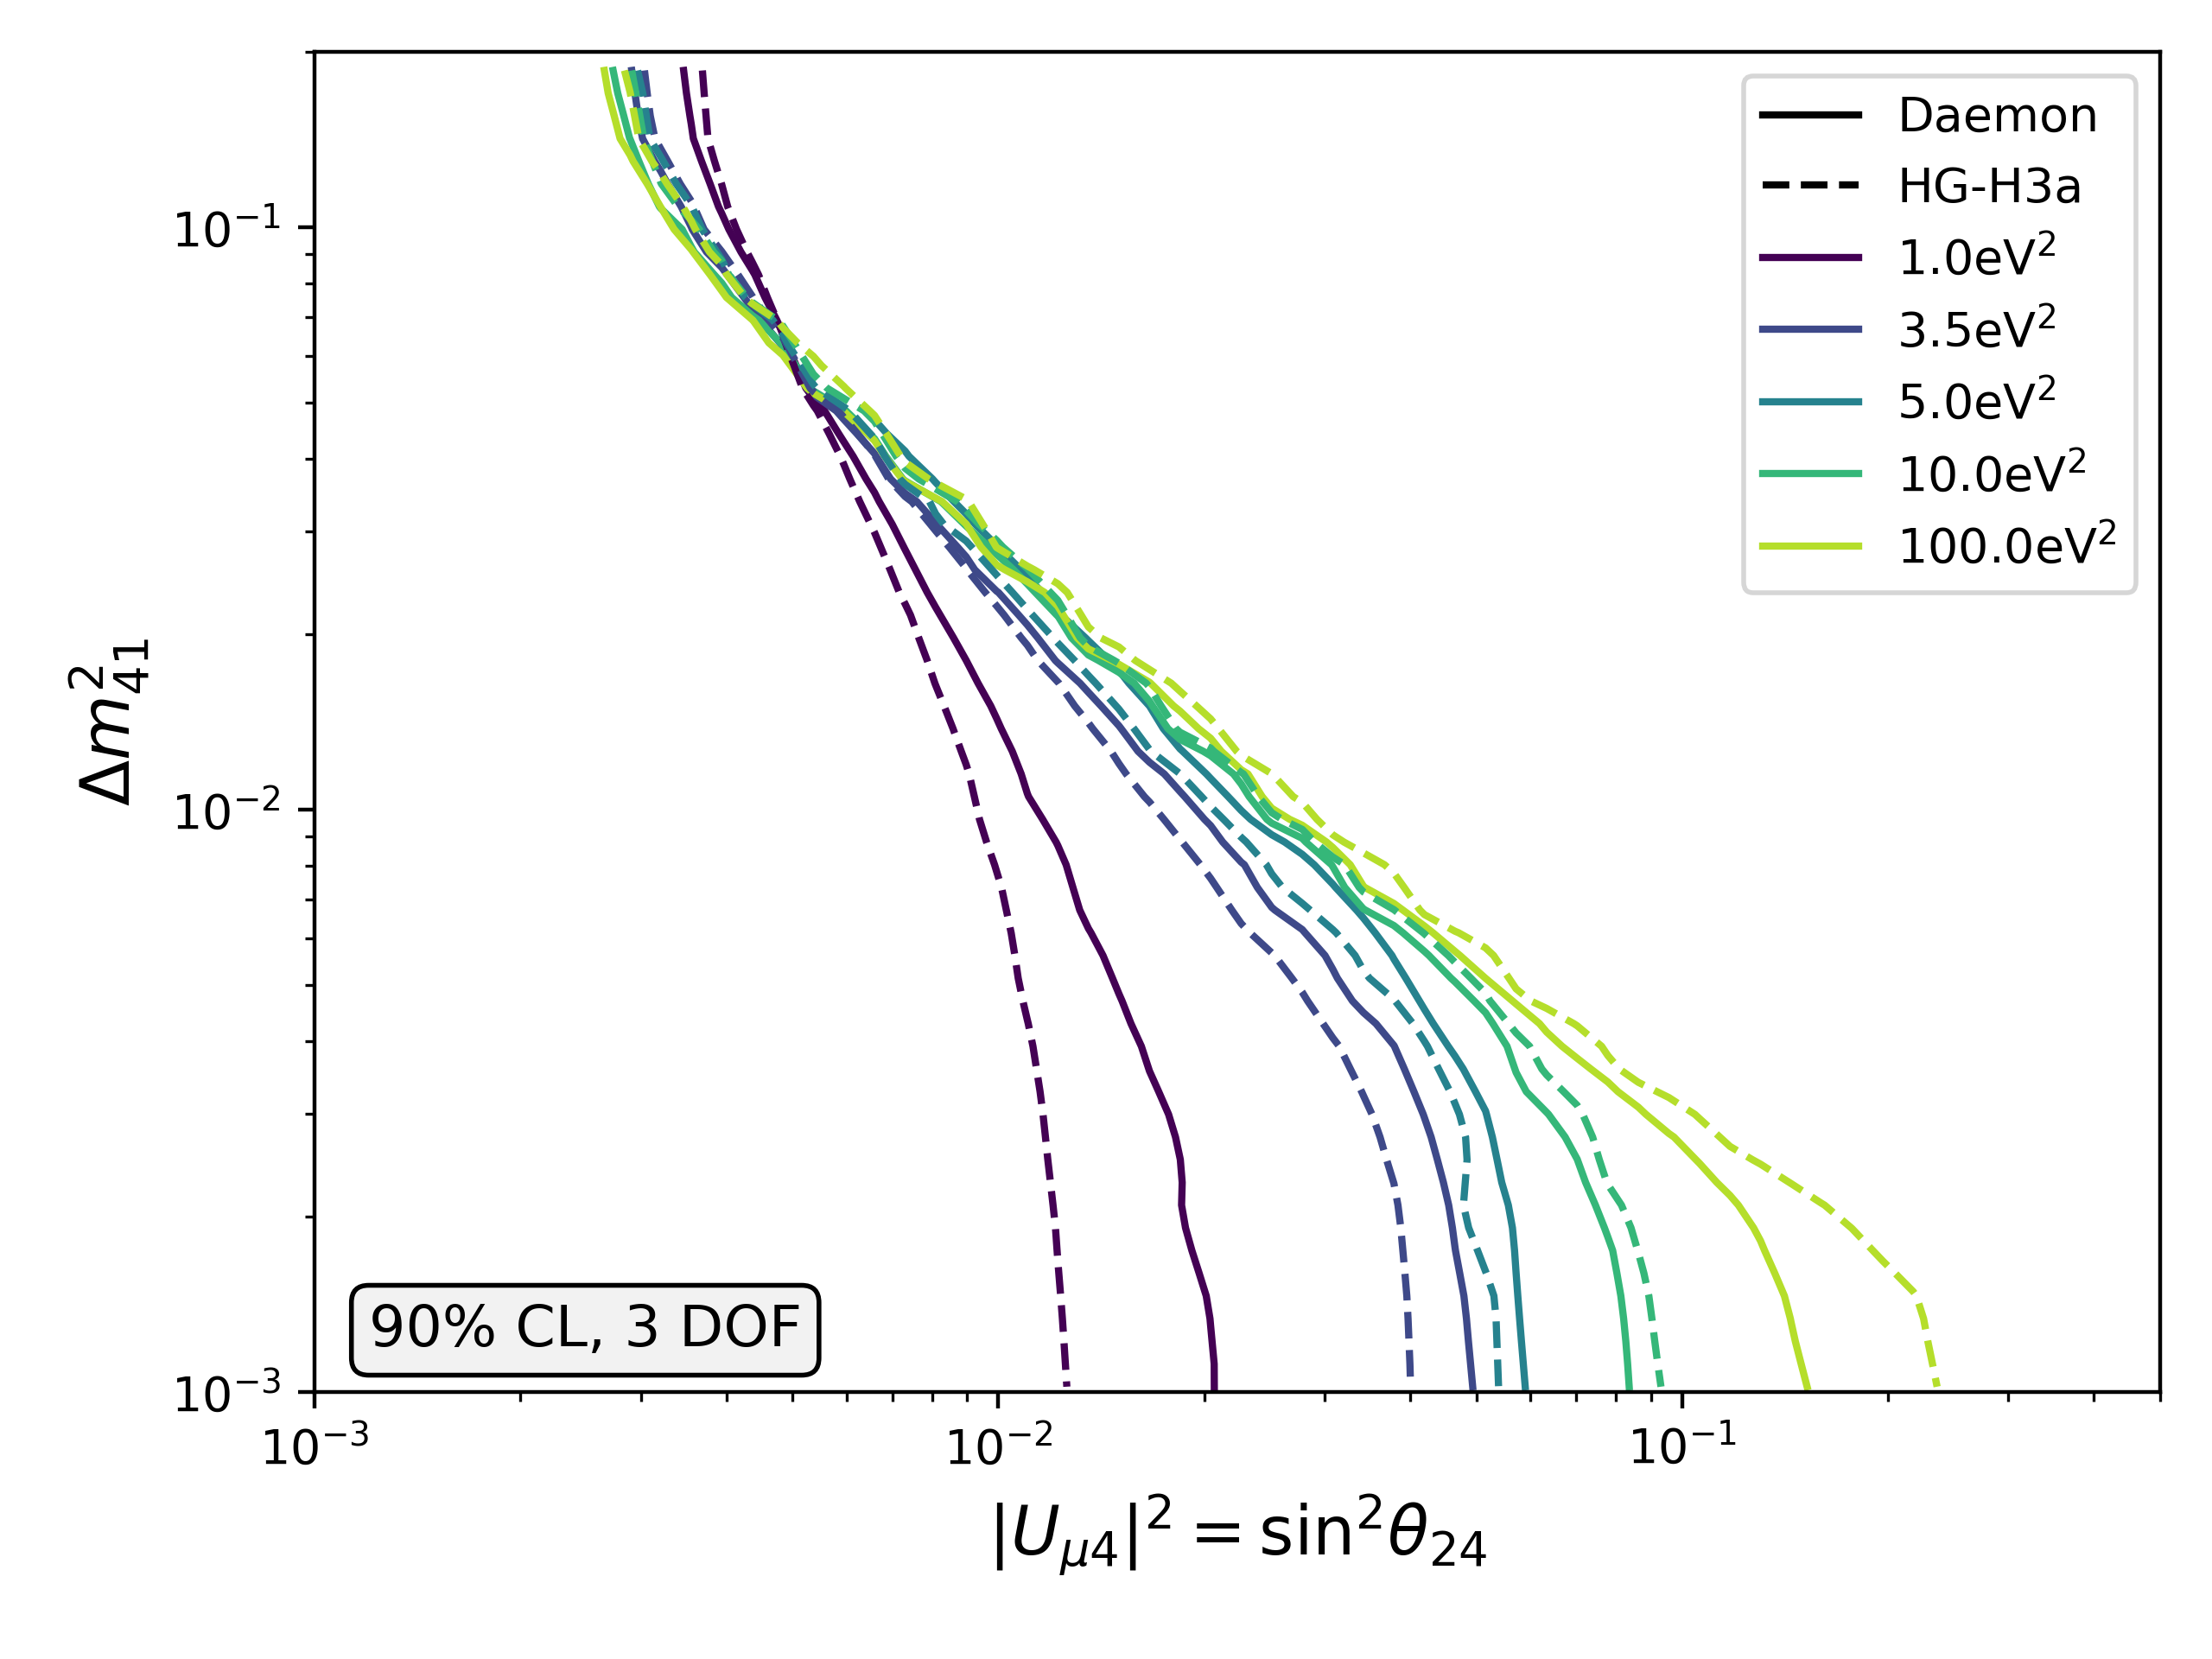
\includegraphics[width=0.7\linewidth]{figures/double_joint_full_daemon_Realization_daemon_Asimov_sterile_0_cl0.9_dof3.png}
    \caption{A comparison of the sensitivities calculated for a daemonflux conventional flux model and the conventional flux model used in the 8-year analysis (labeled as \textit{HG-H3a}).}\label{fig:asimov_model_compare}
\end{figure}


\begin{figure}
    \centering
    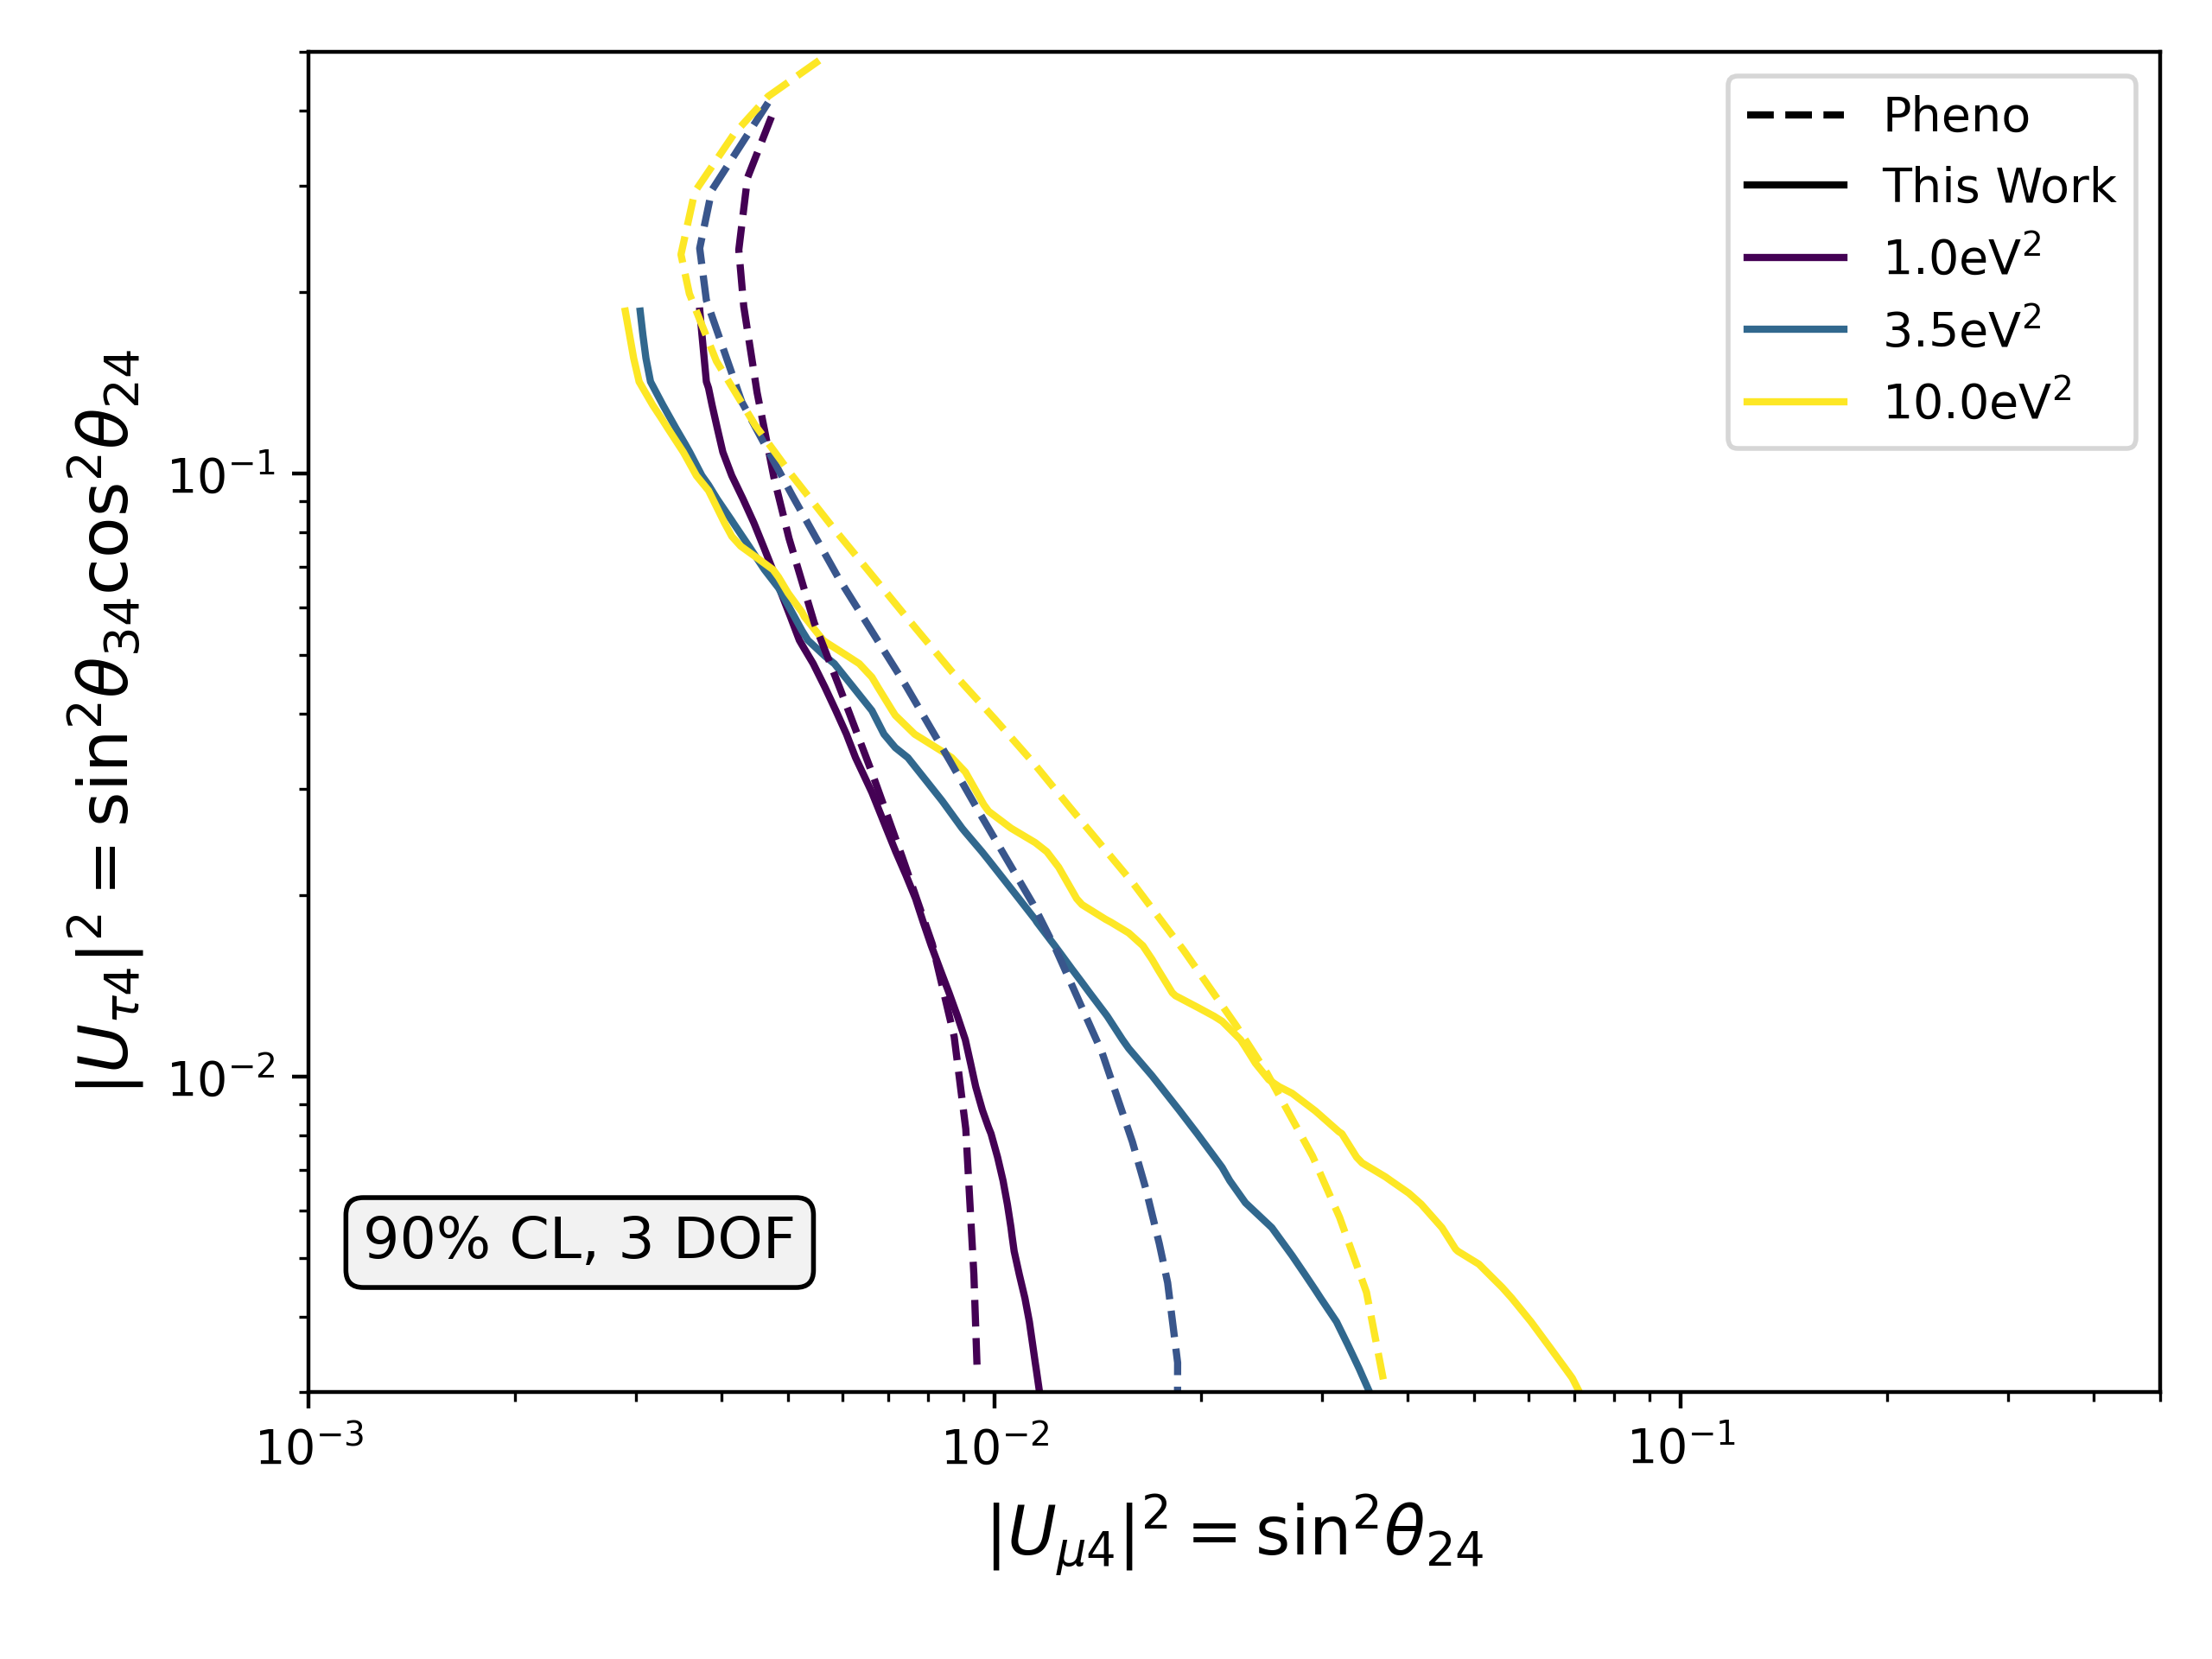
\includegraphics[width=0.45\linewidth]{figures/pheno_joint_asimov_oldairs_Realization_Asimov_sterile_0_cl0.9_dof3.png}%
    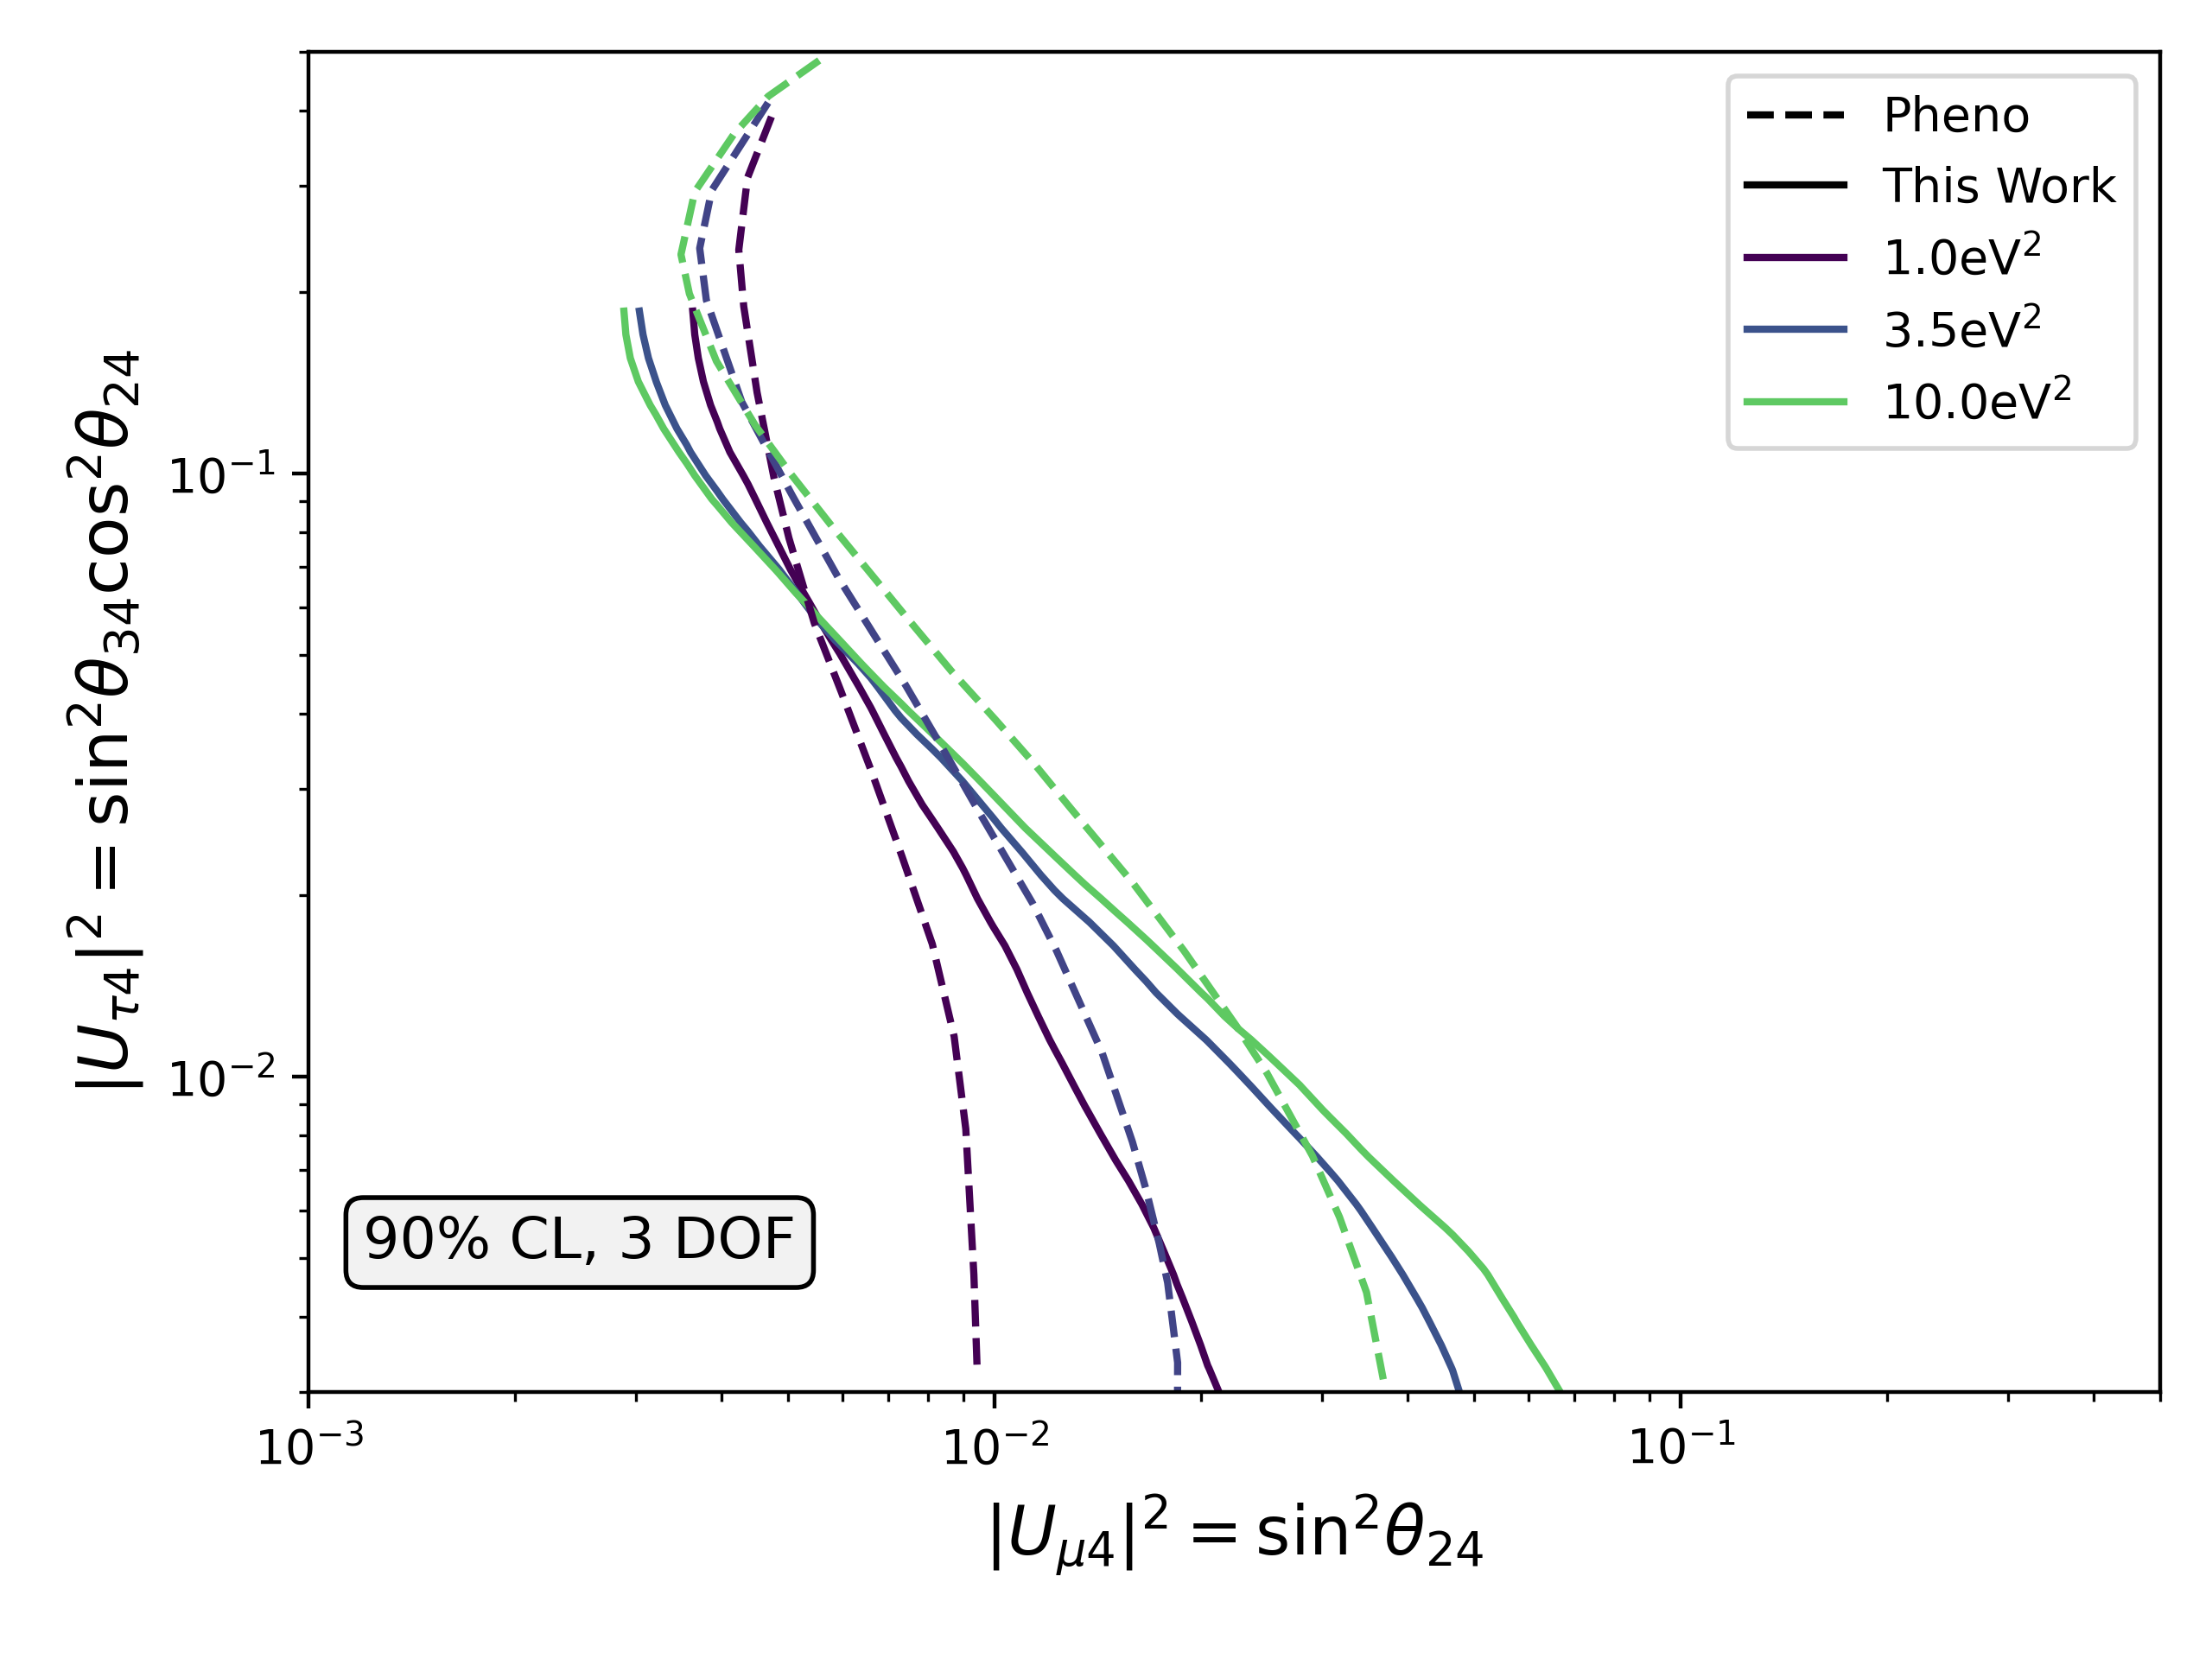
\includegraphics[width=0.45\linewidth]{figures/pheno_joint_daemon_update_Realization_daemon_Asimov_sterile_0_cl0.9_dof3.png}
    \caption{The 90\% confidence level sensitivity contours for this analysis compared with previous phenomenological predictions with three degrees of freedom at $\Delta m_{41}^{2}=$ 1.0 eV$^{2}$, 3.5 eV$^{2}$, and  4.5 eV$^{2}$. On the left, using the 8-year analysis conventional flux model, and on the right using daemonflux.}\label{fig:pheno_compare}
\end{figure}

\begin{figure}
    \centering
    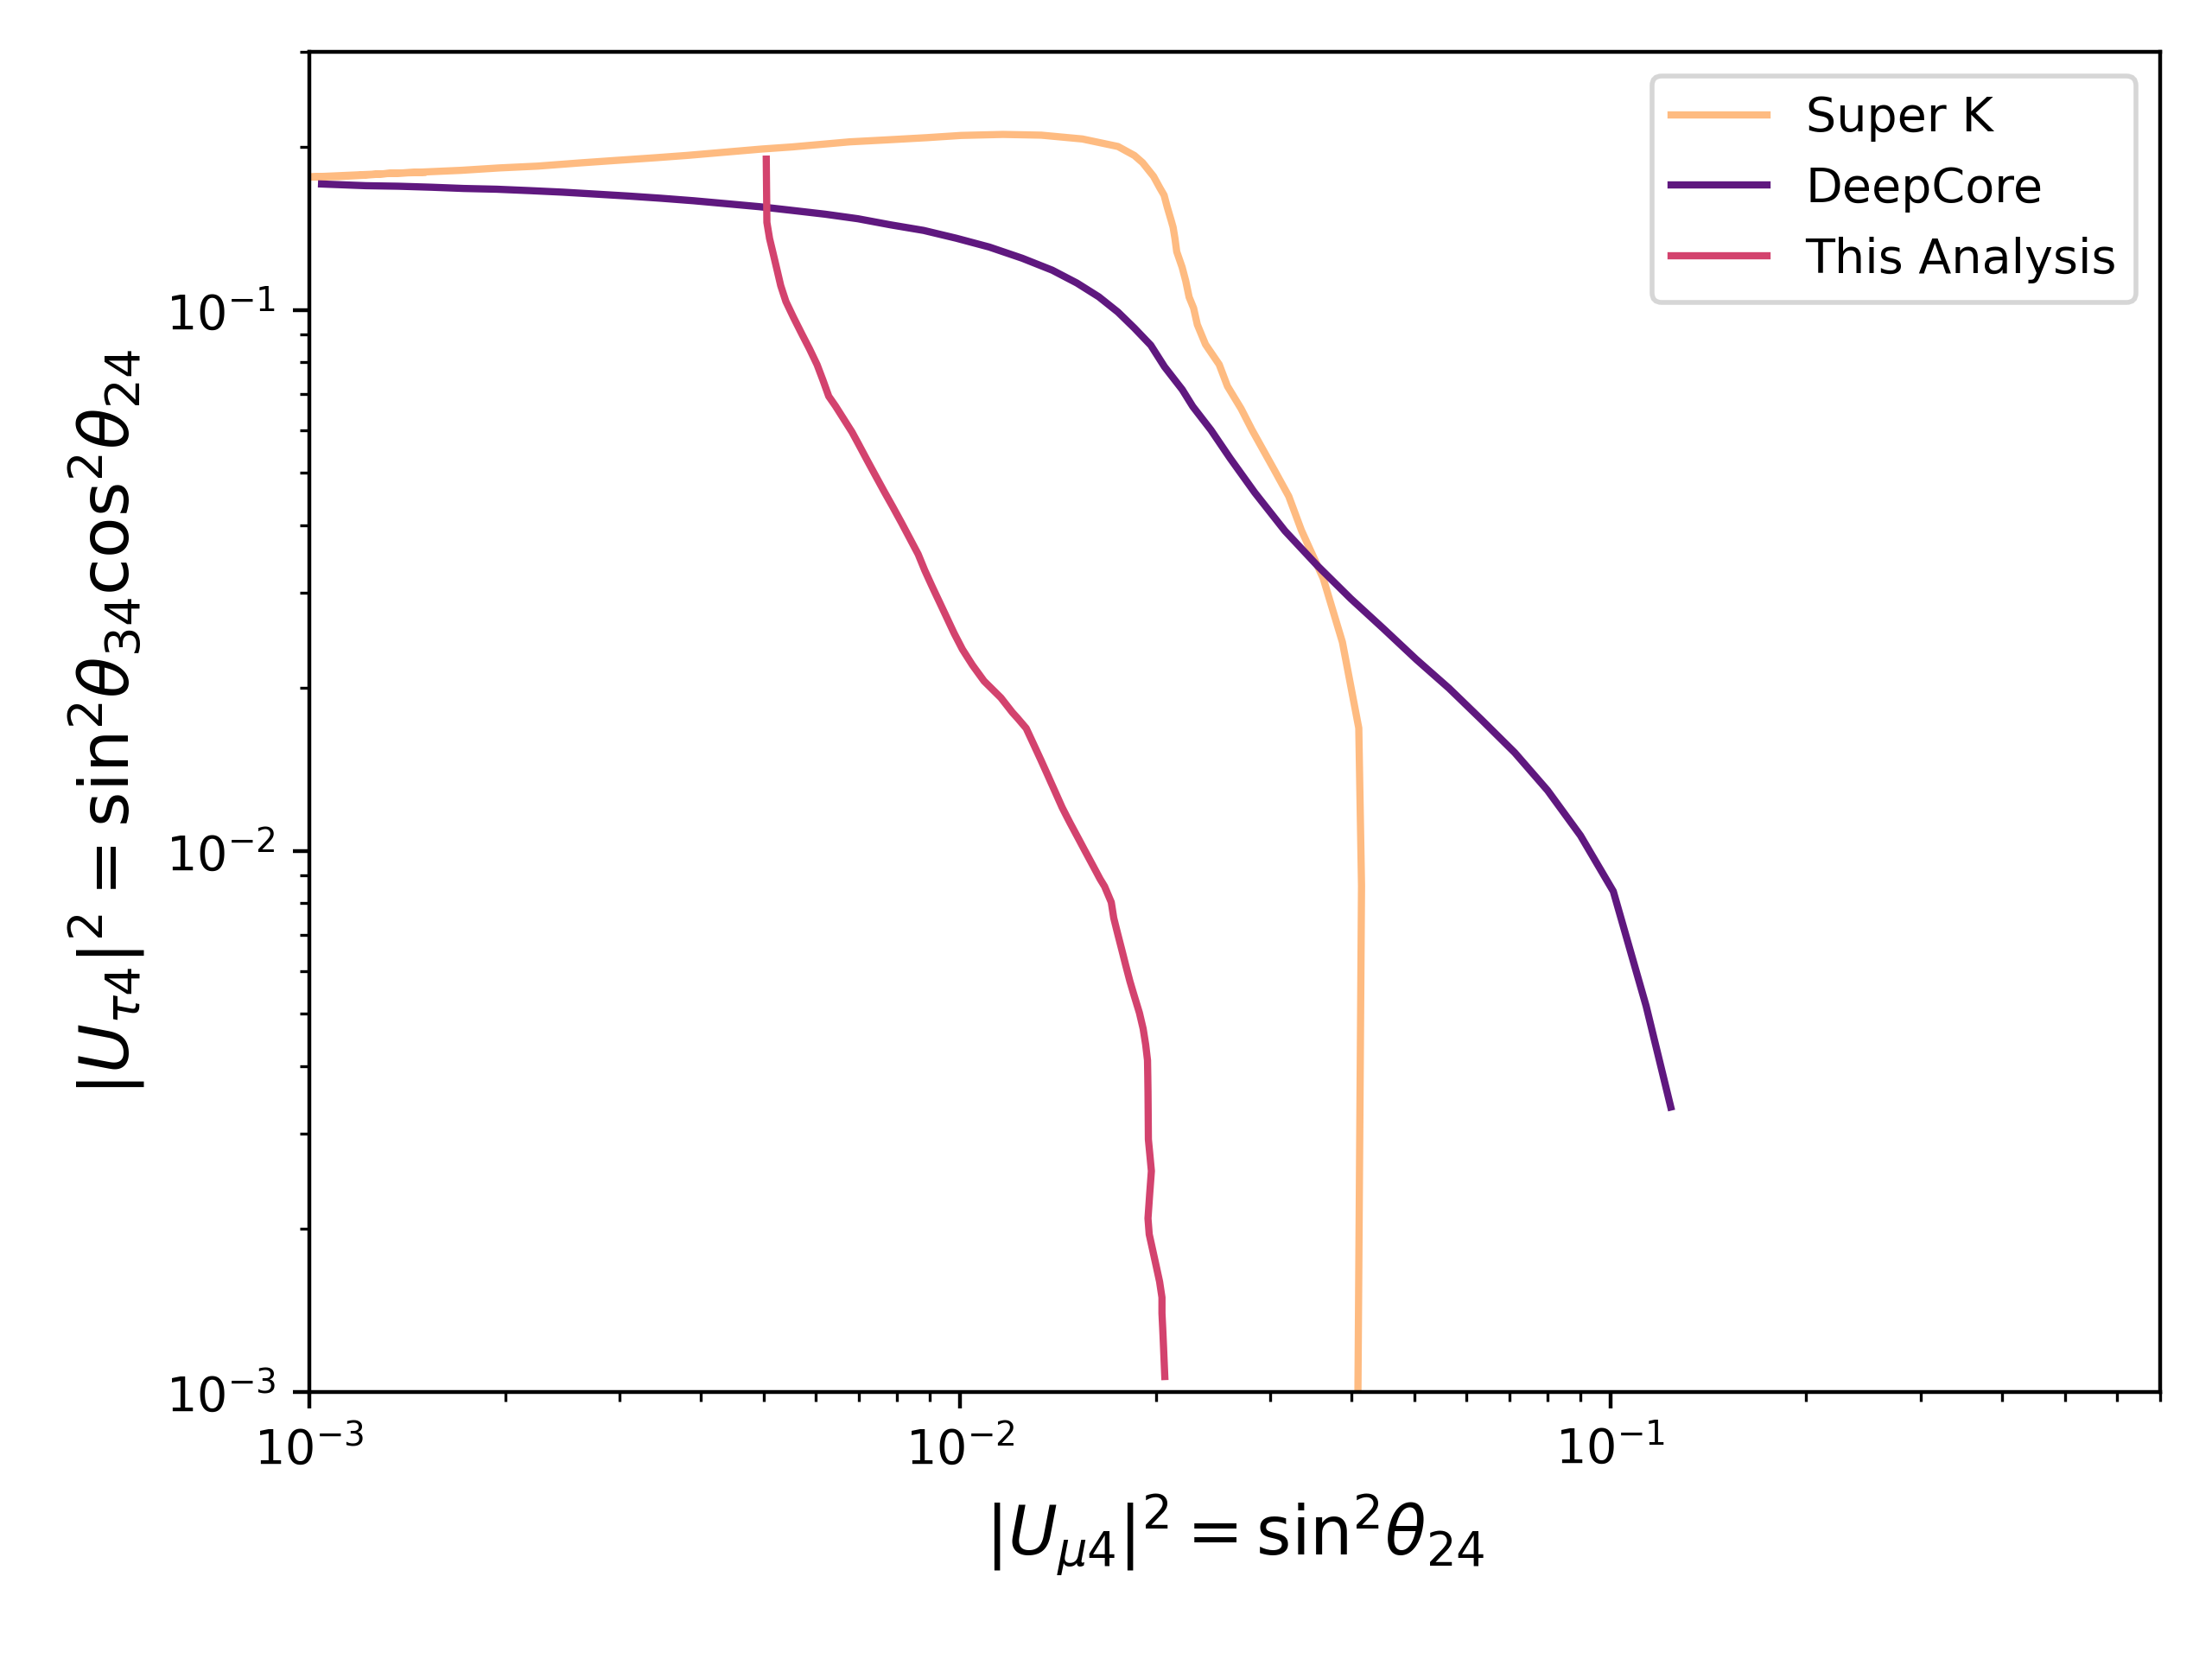
\includegraphics[width=0.45\linewidth]{figures/comparison.png}%
    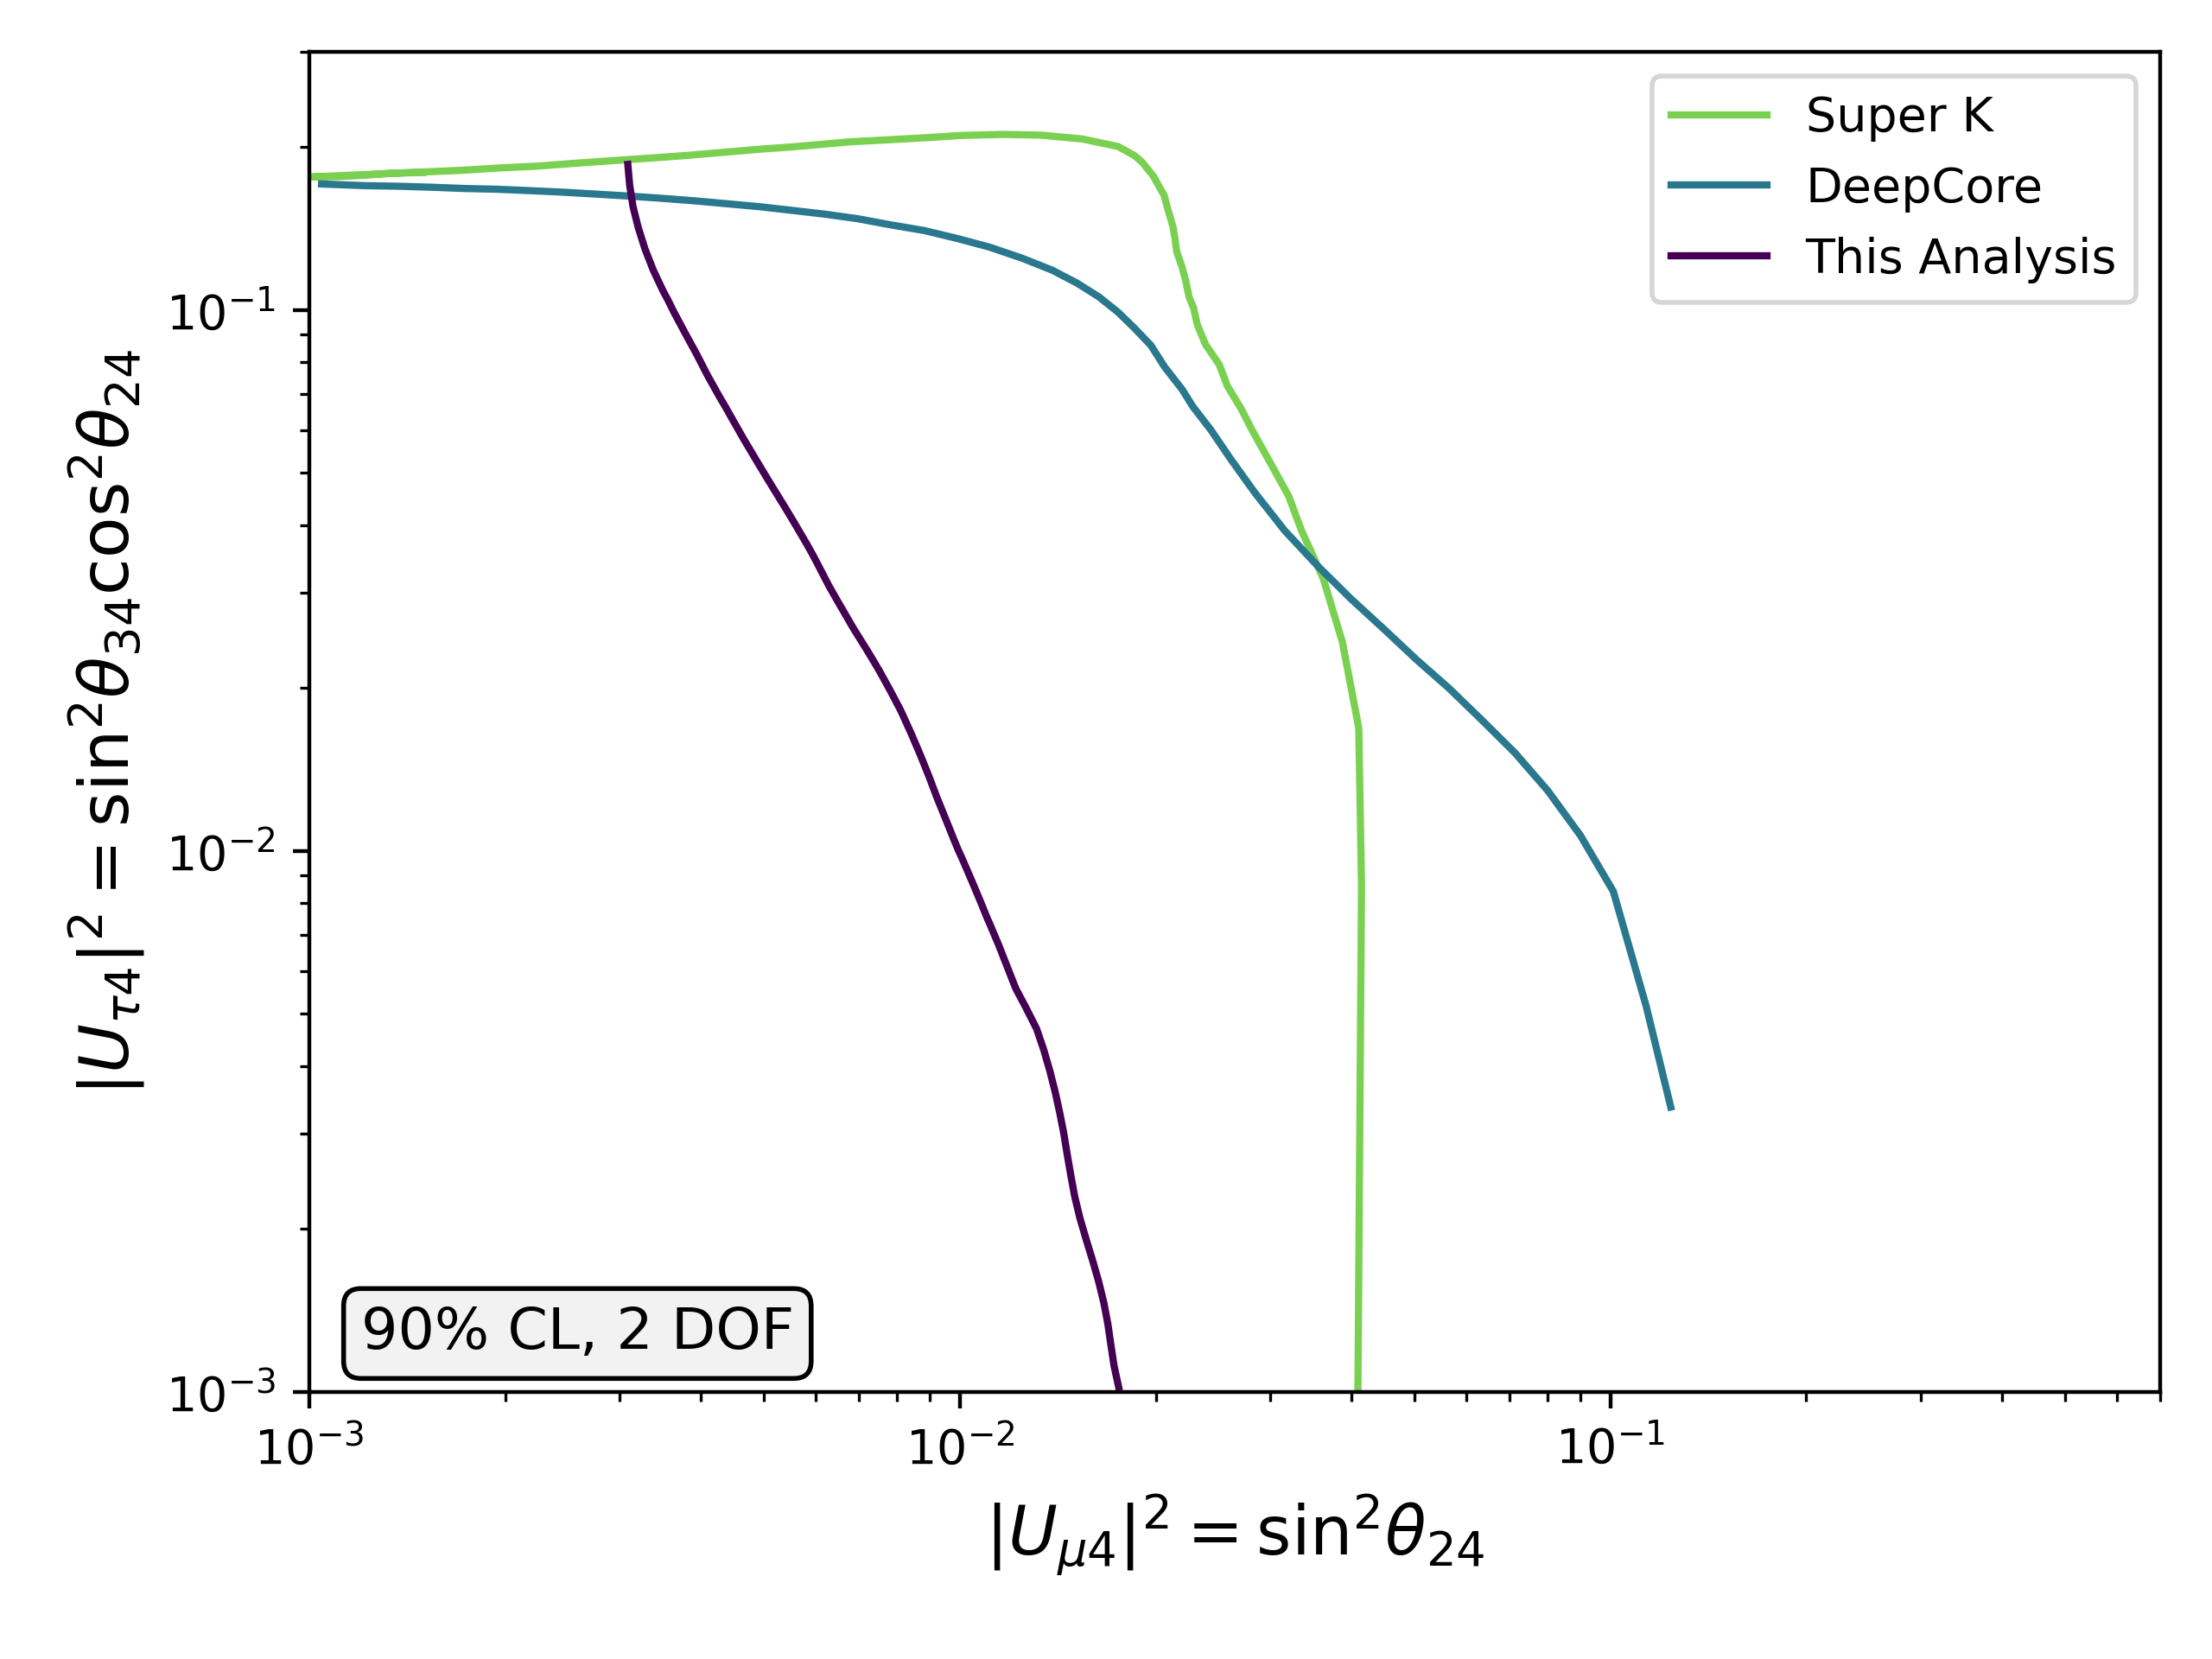
\includegraphics[width=0.45\linewidth]{figures/comparison_updated.png}
    \caption{On the left (right) the 90\% confidence level sensitivity contours for this analysis with two degrees of freedom at $\Delta m_{41}^{2}=$ 1.0 eV$^{2}$ using the same conventional flux model as in the 8-year analysis (daemonflux). Sensitivities from DeepCore~\cite{Aartsen_2017_dc} and Super-K~\cite{PhysRevD.91.052019} at 1.0eV$^{2}$ are provided for comparison.}\label{fig:experiment_compare}
\end{figure}


\subsection{Median Sensitivities}


We simulated ~80 experimental results assuming no new physics by applying Poissonian statistical fluctuations on a nominal event rate.
A full fit scan was then carried out for each of these pseudo-experiments, and the exclusion contours were drawn for each.
The median location of the contour, the bands containing 68\% of the contours, and the bands containing 95\% of contours were then calculated for contours at 90\% and 95\% confidence level. 
The bands over $\abs{U_{\mu 4}}^{2}$ are calculated as a function of $\abs{U_{\tau}4}^{2}$ for each explored mass squared splitting. 
They are then shown in Figure~\ref{fig:brazil} for contours at 90\% CL (top) and 95\% CL (bottom).
The median sensitivity was observed to converge to the Asimov sensitivity: suggesting Wilks' theorem is valid here. 


\begin{figure}
    \centering
    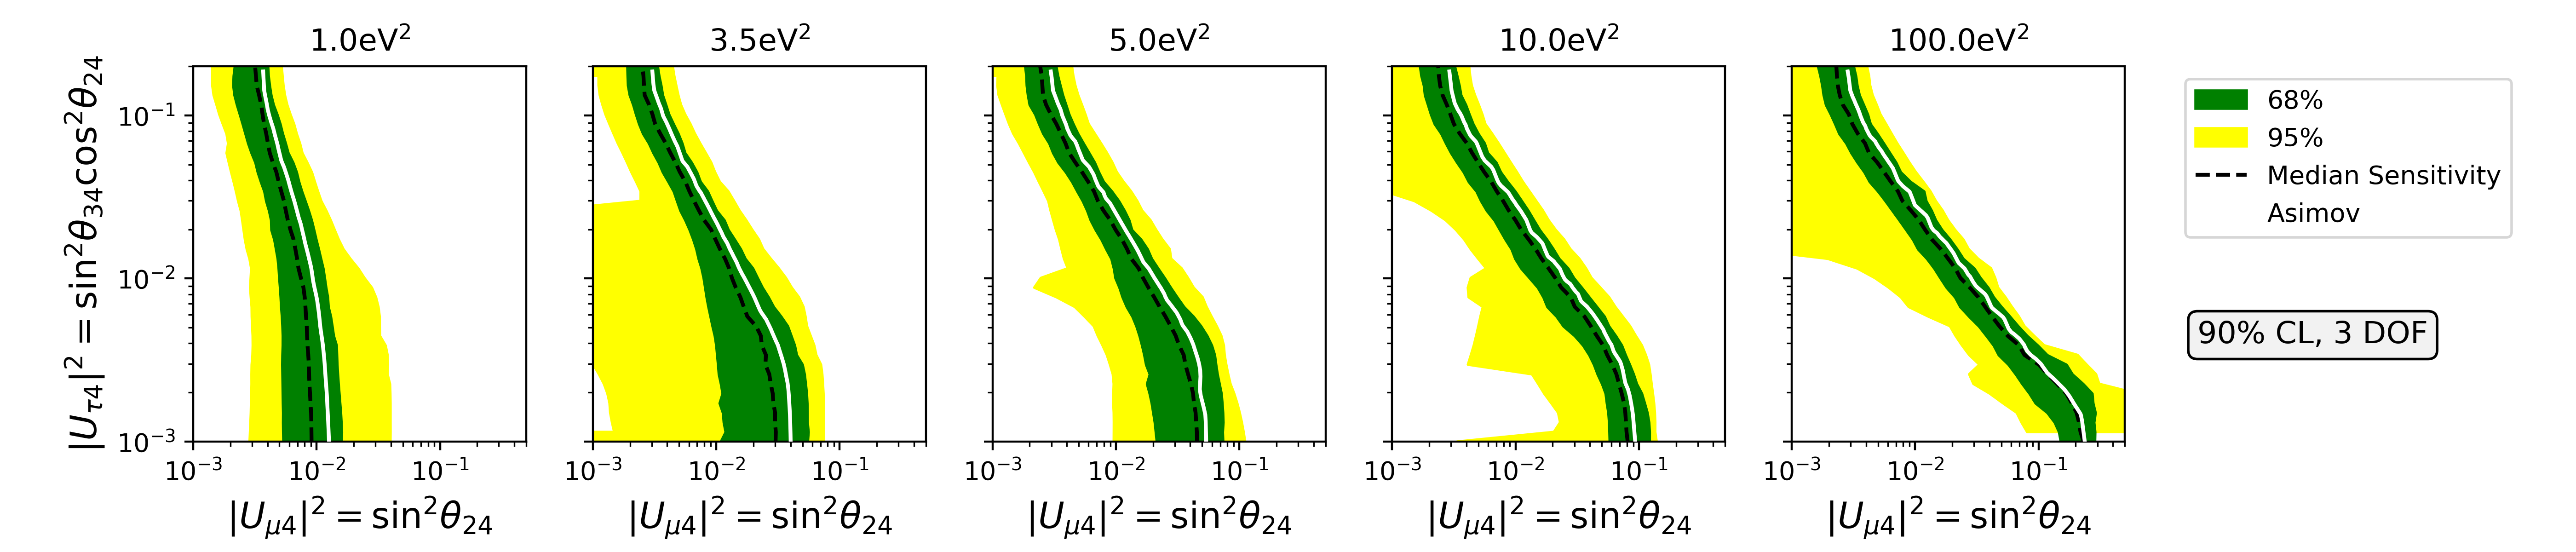
\includegraphics[width=0.95\linewidth]{figures/median_sense_cl0.9.png}\\
    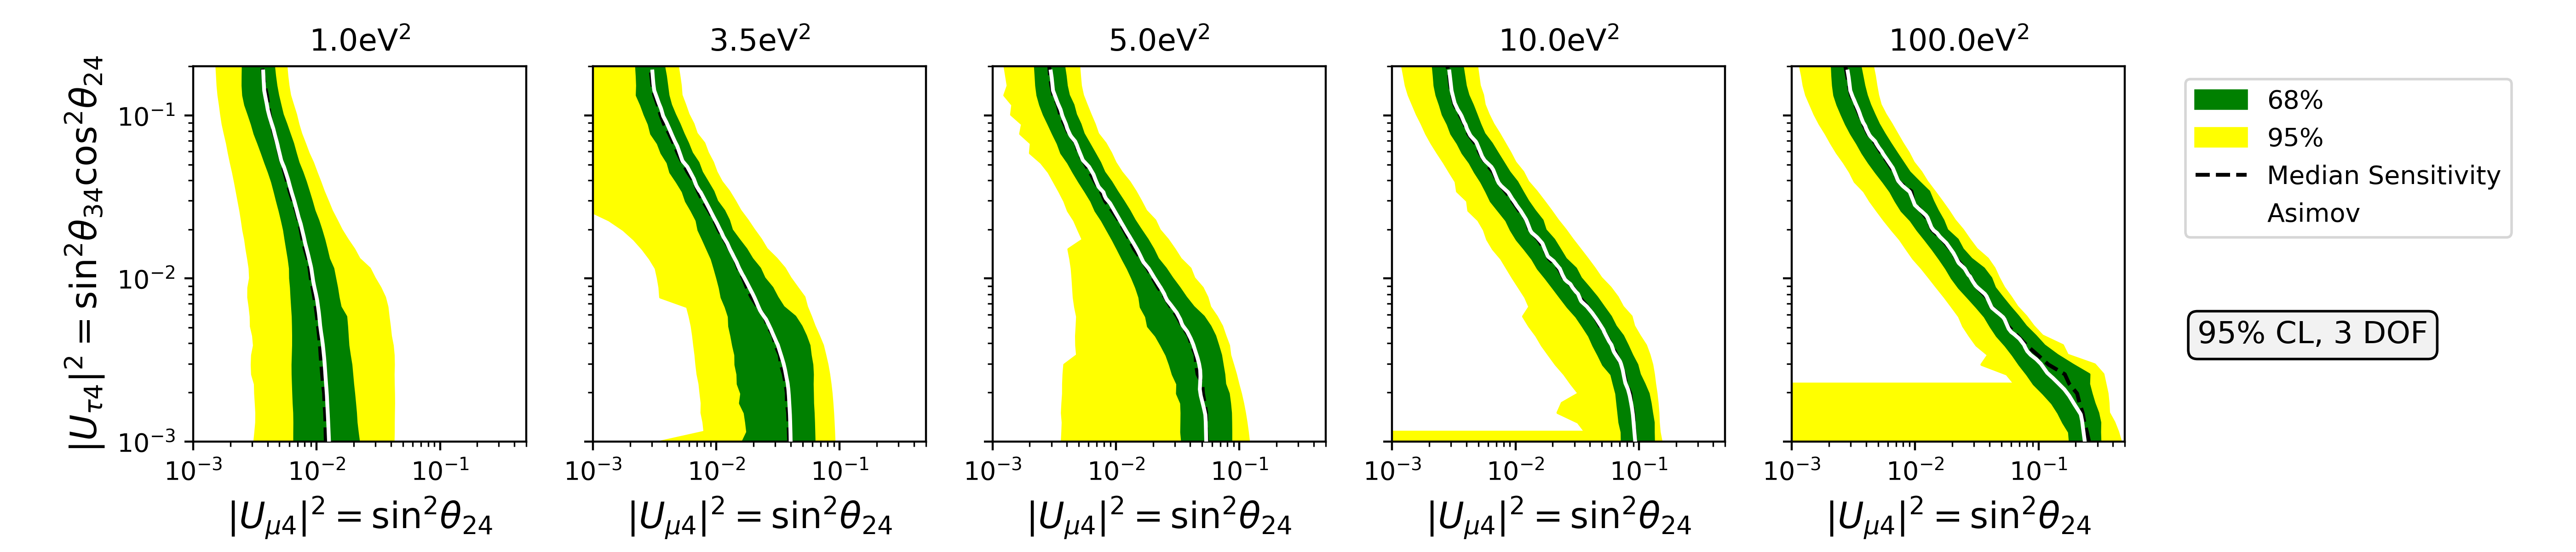
\includegraphics[width=0.95\linewidth]{figures/median_sense_cl0.95.png}
    \caption{``Brazil Bands'' for 90\% CL contours (top) and 95\% CL contours (bottom).}\label{fig:brazil}
\end{figure}

\section{Mismodeling Tests}

There is always the possibility that an inaccurate model of some process could mimic the signatures of a 3+1 sterile neutrino model. 
Several possible sources of such a mismodeling were investigated. 

\subsection{Conventional Neutrino Flux Mismodeling}\label{fig:flux_mismod}

Newer high-energy IceCube oscillations analyses had begun to adopt the daemonflux~\cite{yanez2023daemonflux} cosmic ray and conventional neutrino model at the start of this analysis. 
To test its relevance we generated a pseudo-experiment where daemonflux is the true neutrino flux with no new physics. 
Then, fits were run assuming a neutrino flux resulting from a Hillas-Gaisser H3a cosmic ray model~\cite{GAISSER2012801}, Sibyll2.3c interaction model~\cite{Riehn:2017mfm}, and an AIRS-like atmosphere model~\cite{airs_ref}. 
This is the same as the model used in the 8-year IceCube sterile search~\cite{Aartsen_2020, Aartsen_2020_prd}. 
The result of a joint-fit are shown in Figure~\ref{fig:uhoh_mismodel}.
In this case, a 3+1 sterile model is preferred over the injected (null) physics values with a significance of $-2(\mathcal{L}_{best}-\mathcal{L}_{null})=4.68$. 

\begin{figure}  
    \centering
    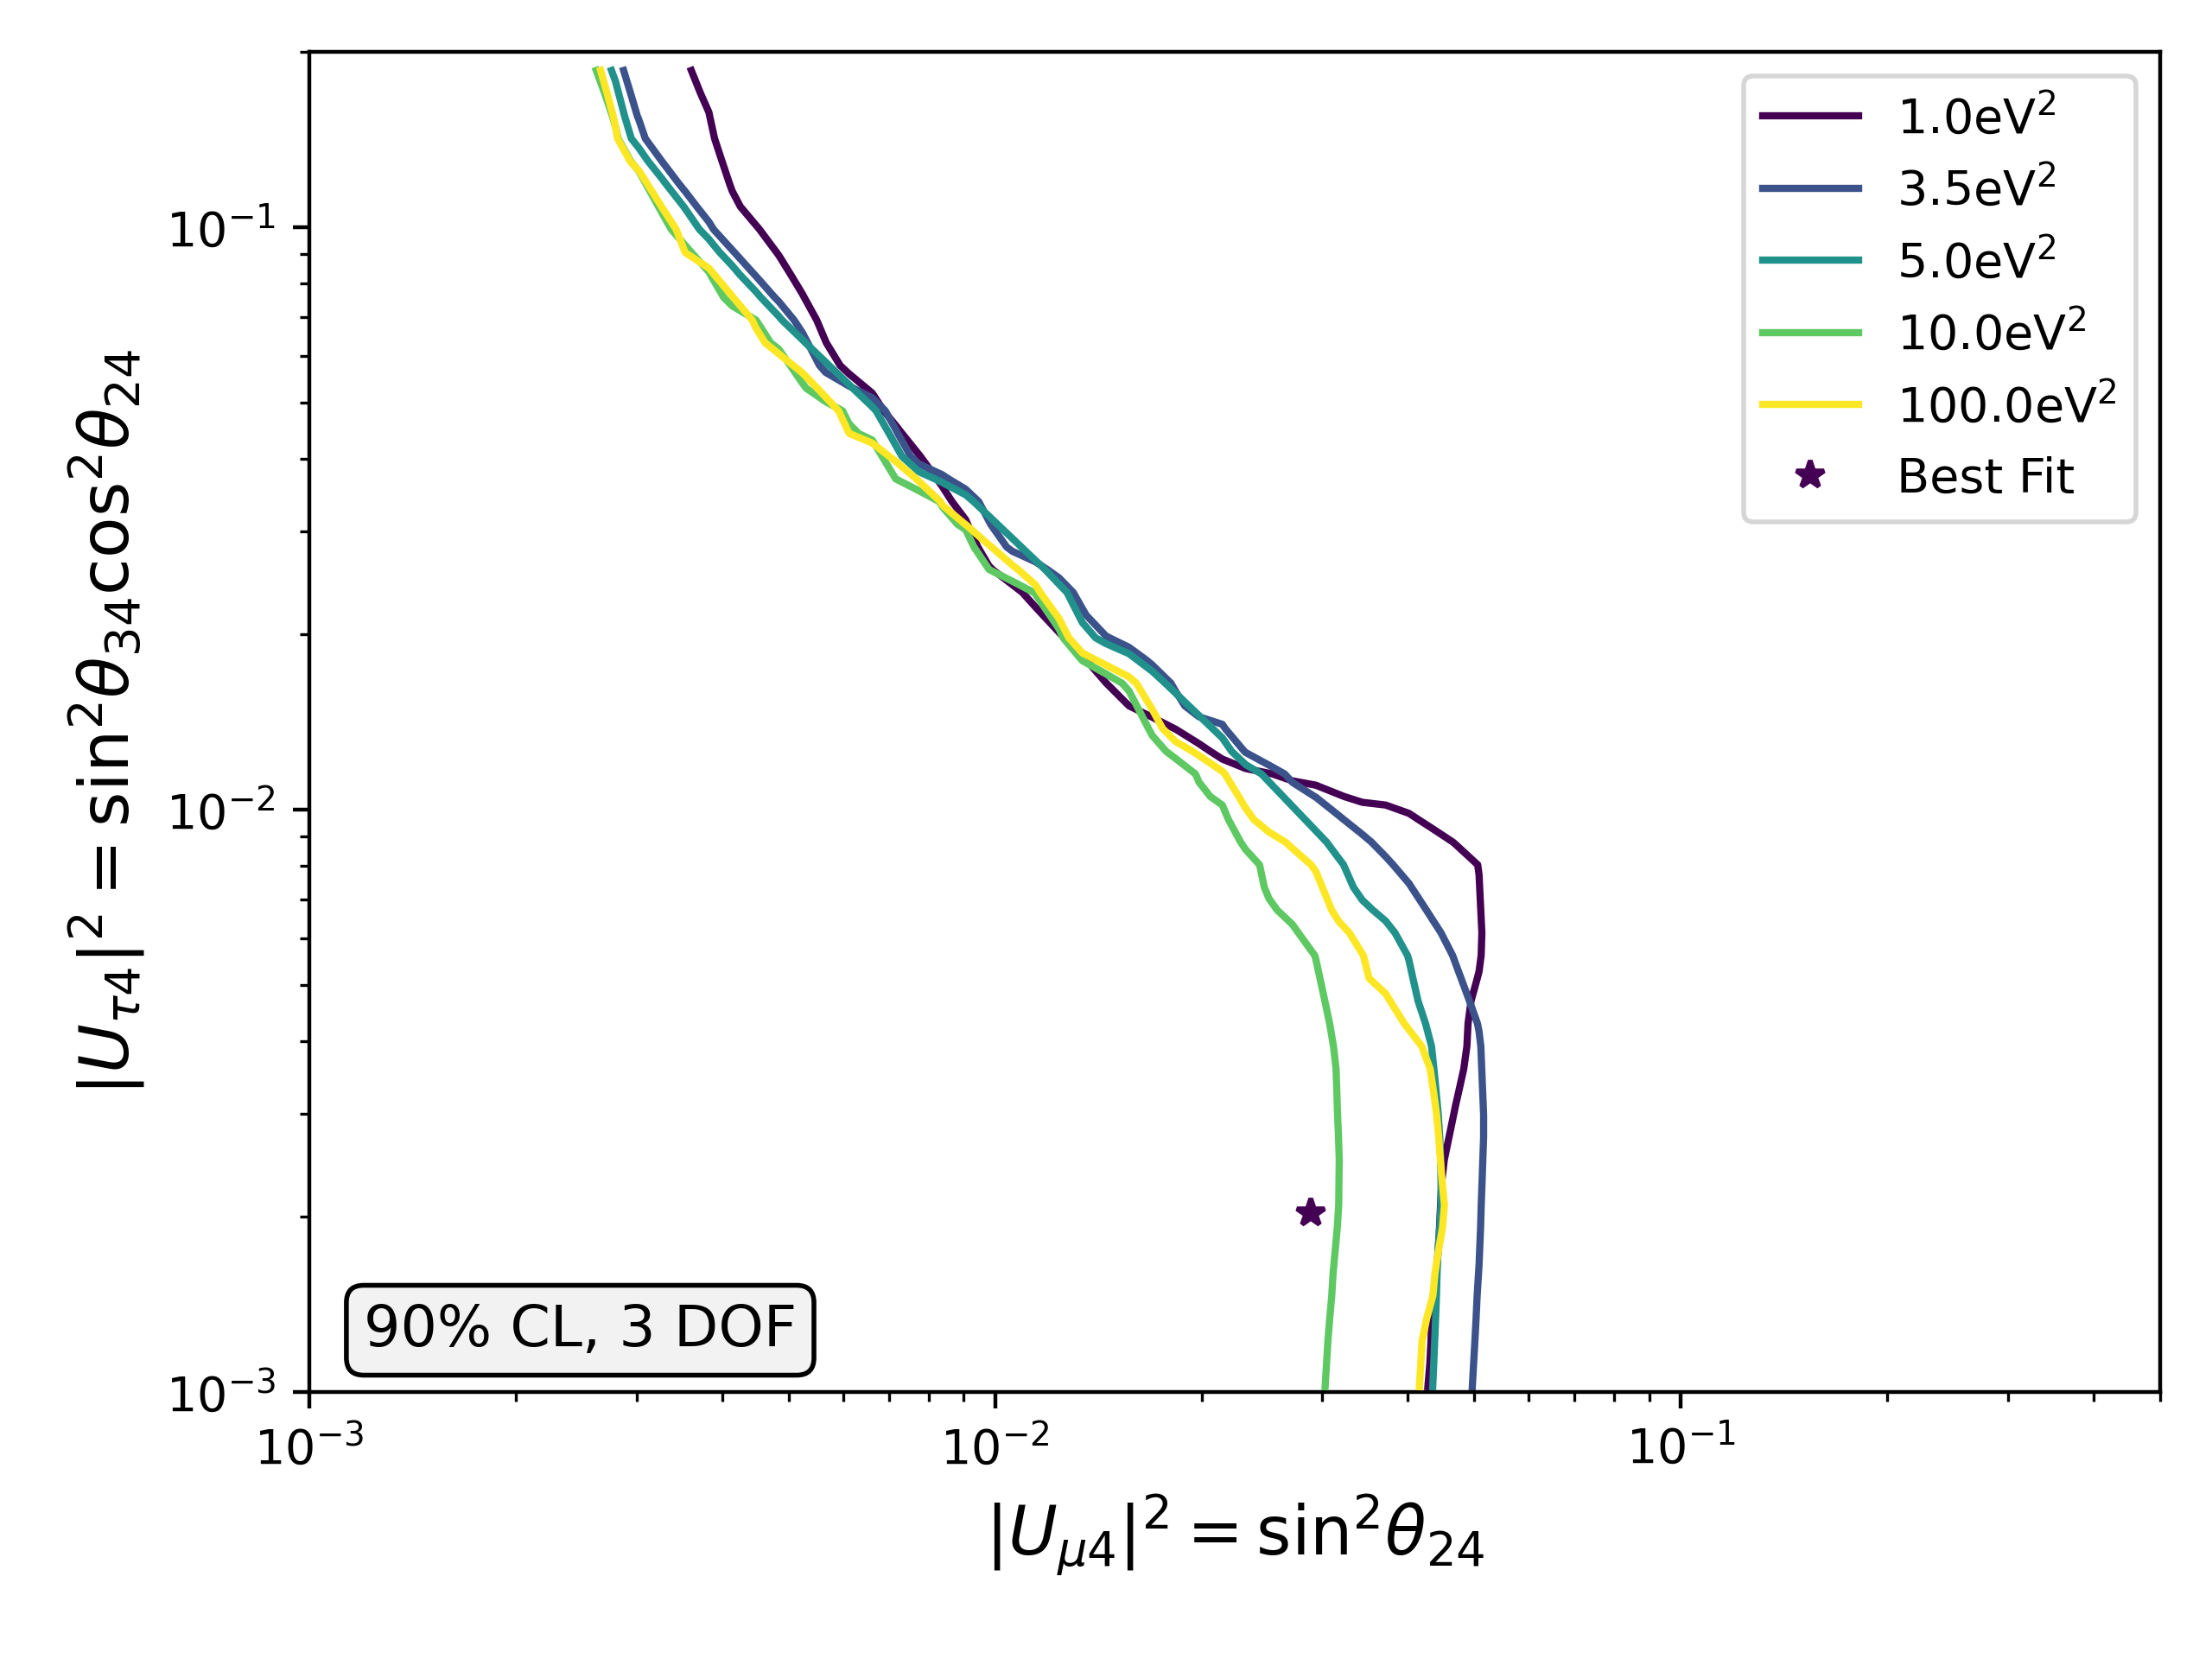
\includegraphics[width=0.7\linewidth]{figures/joint_daemon_mismodel_Realization_daemon_Asimov_sterile_0_cl0.9_dof3.png}
    \caption{The 90\% CL contours for three degrees of freedom. A daemonflux flux is injected and a flux model consistent with the 8-year IceCube sterile search is assumed. The fit prefers the 3+1 sterile neutrino model at a significance of $-2(\mathcal{L}_{best}-\mathcal{L}_{null})=4.68$.}\label{fig:uhoh_mismodel}
\end{figure}

Further, two similar fit-scans were carried out using only tracks. 
In the first, the fit-scan is carried out fixing $\abs{U_{\tau 4}}^{2}$ to zero but allowing a more fine scan in $\Delta m_{41}^{2}$; the second is done in a three-degree fit over $(\abs{U_{\mu 4}}^{2})$, $(\abs{U_{\tau 4}}^{2})$, and $\Delta m_{41}^{2}$. 
These scans are shown in Figure~\ref{fig:uhoh_mismodel_worse}; in the 2D scan a spurious closed-contour result is recovered at the 90\% confidence level. 
This suggests that if daemonflux is a better description of the truth, then assuming the model used in the 8-year IceCube sterile analysis is likely to yield spurious 3+1 signals given no new physics, or artificially strong signals given sterile neutrinos.

\begin{figure}  
    \centering
    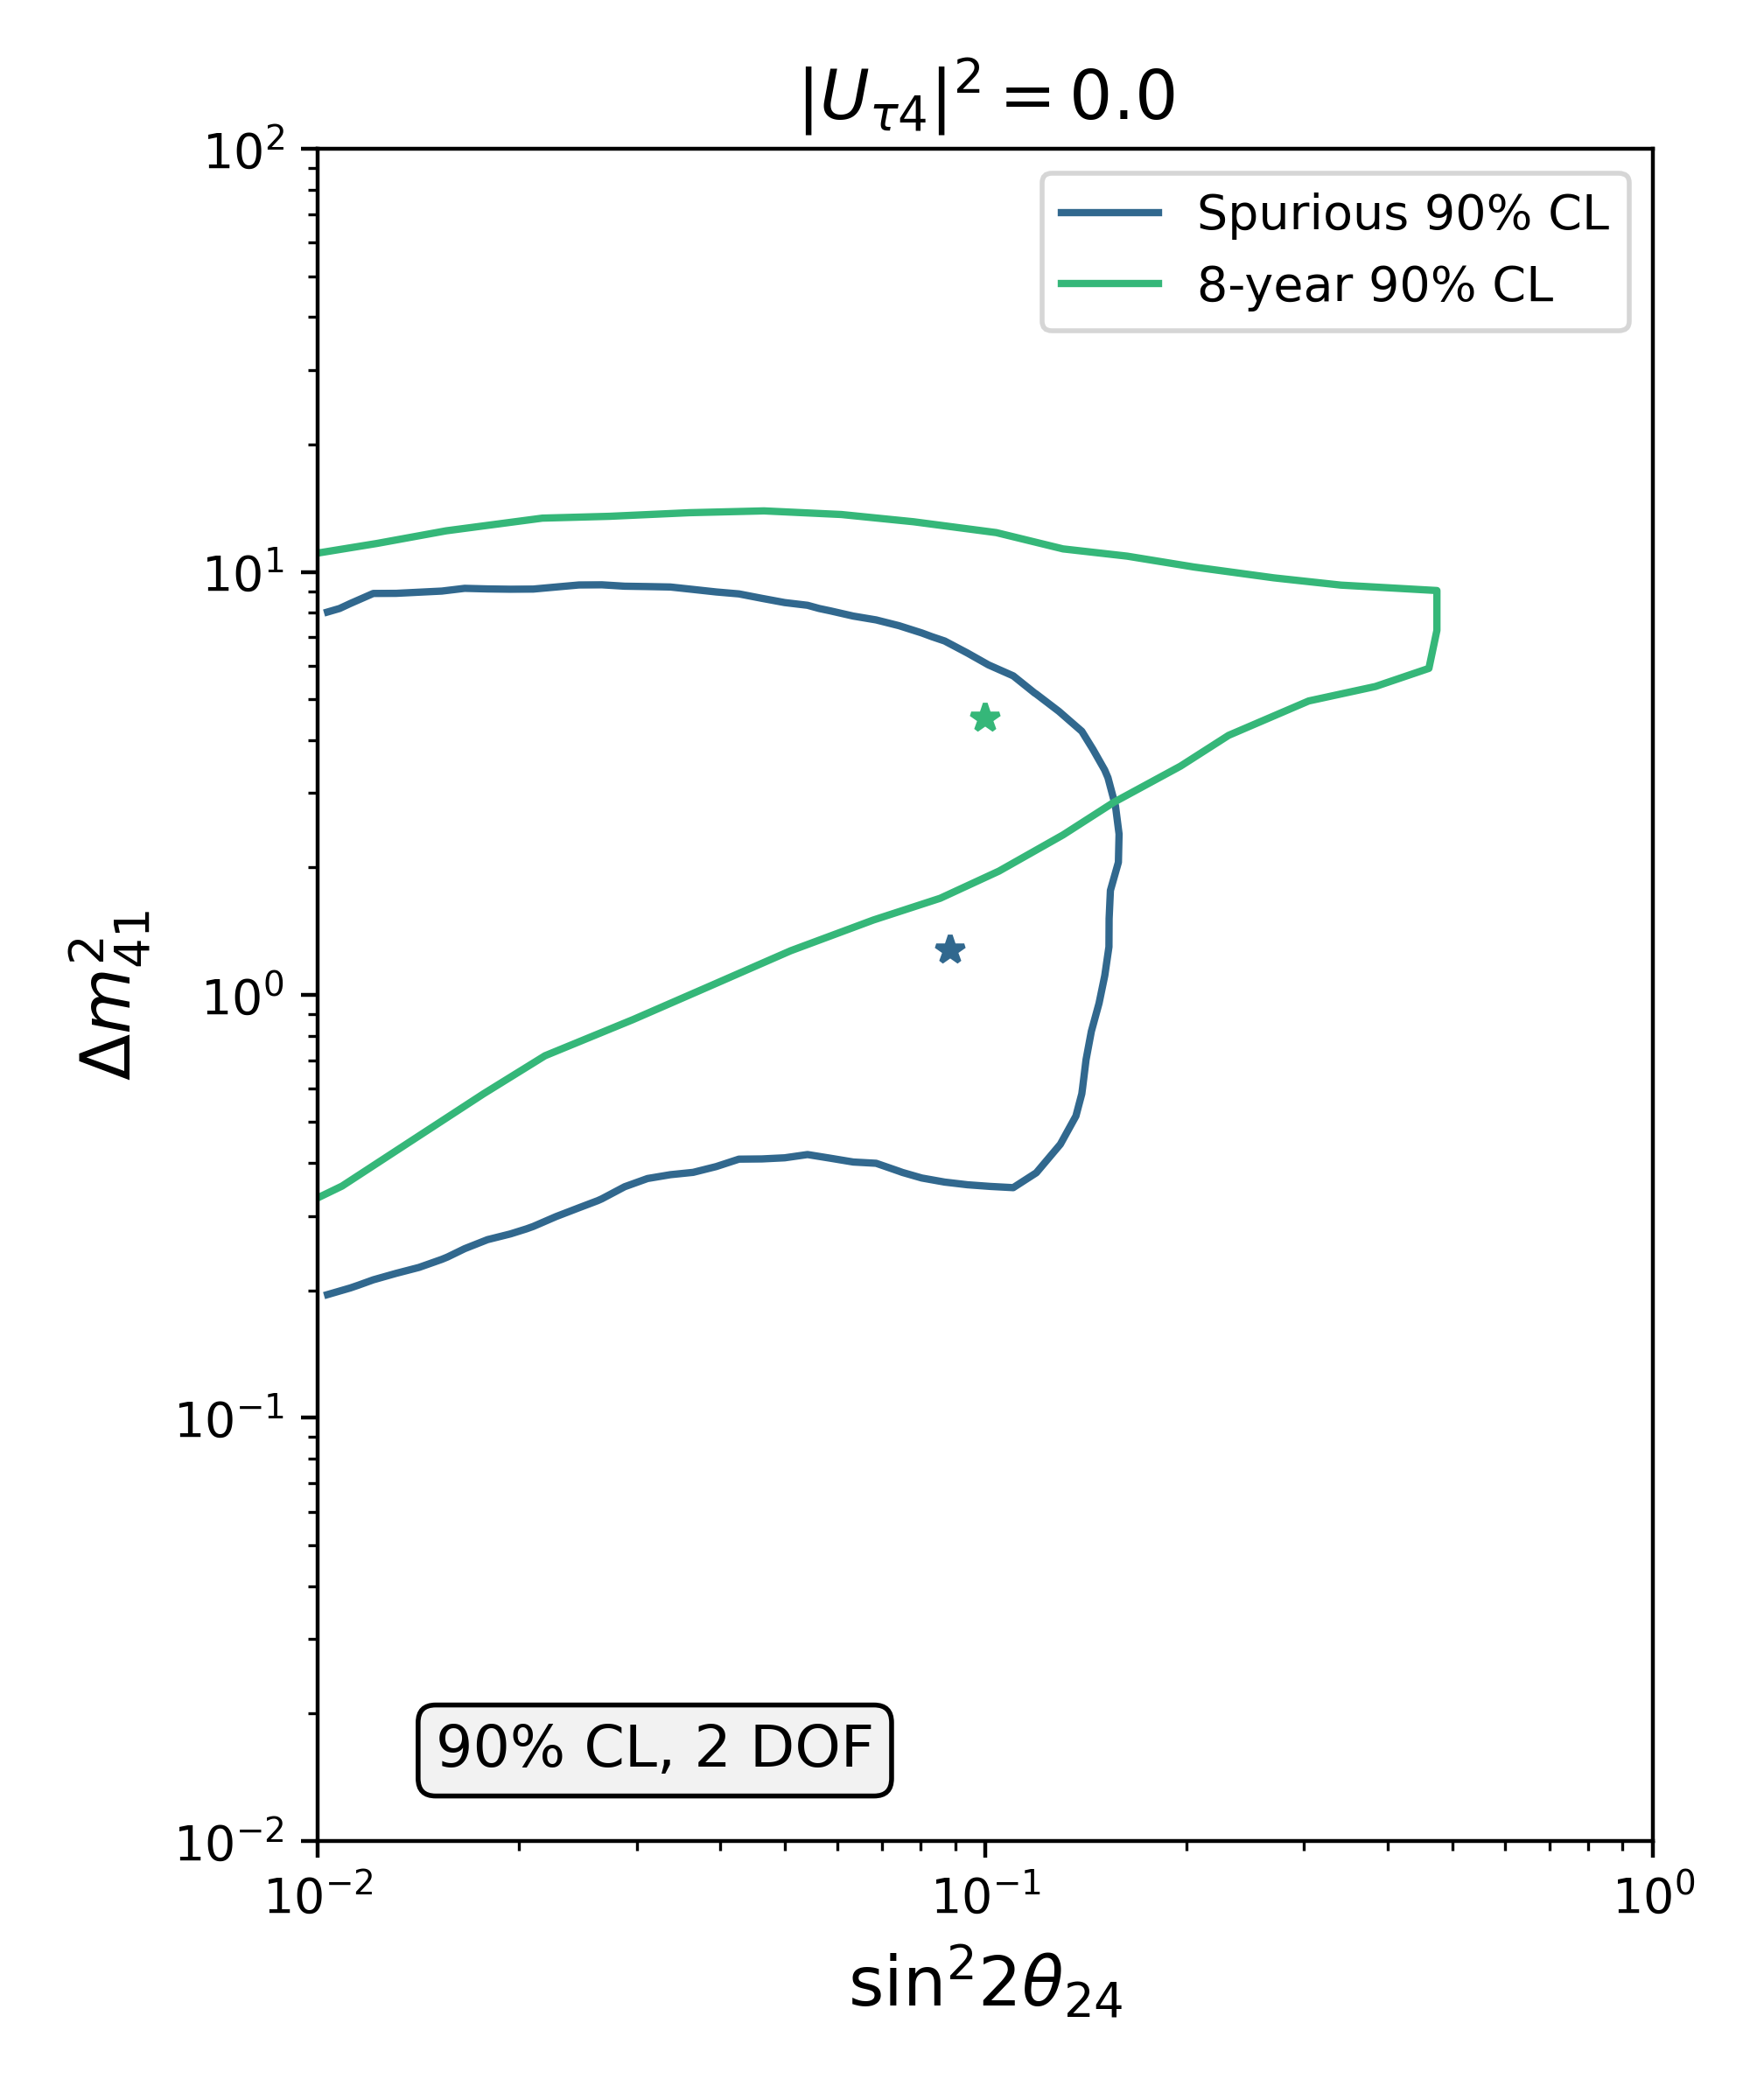
\includegraphics[width=0.45\linewidth]{figures/track_daemon_mismodel_Realization_daemon_Asimov_sterile_0_cl0.9_dof2.png}
    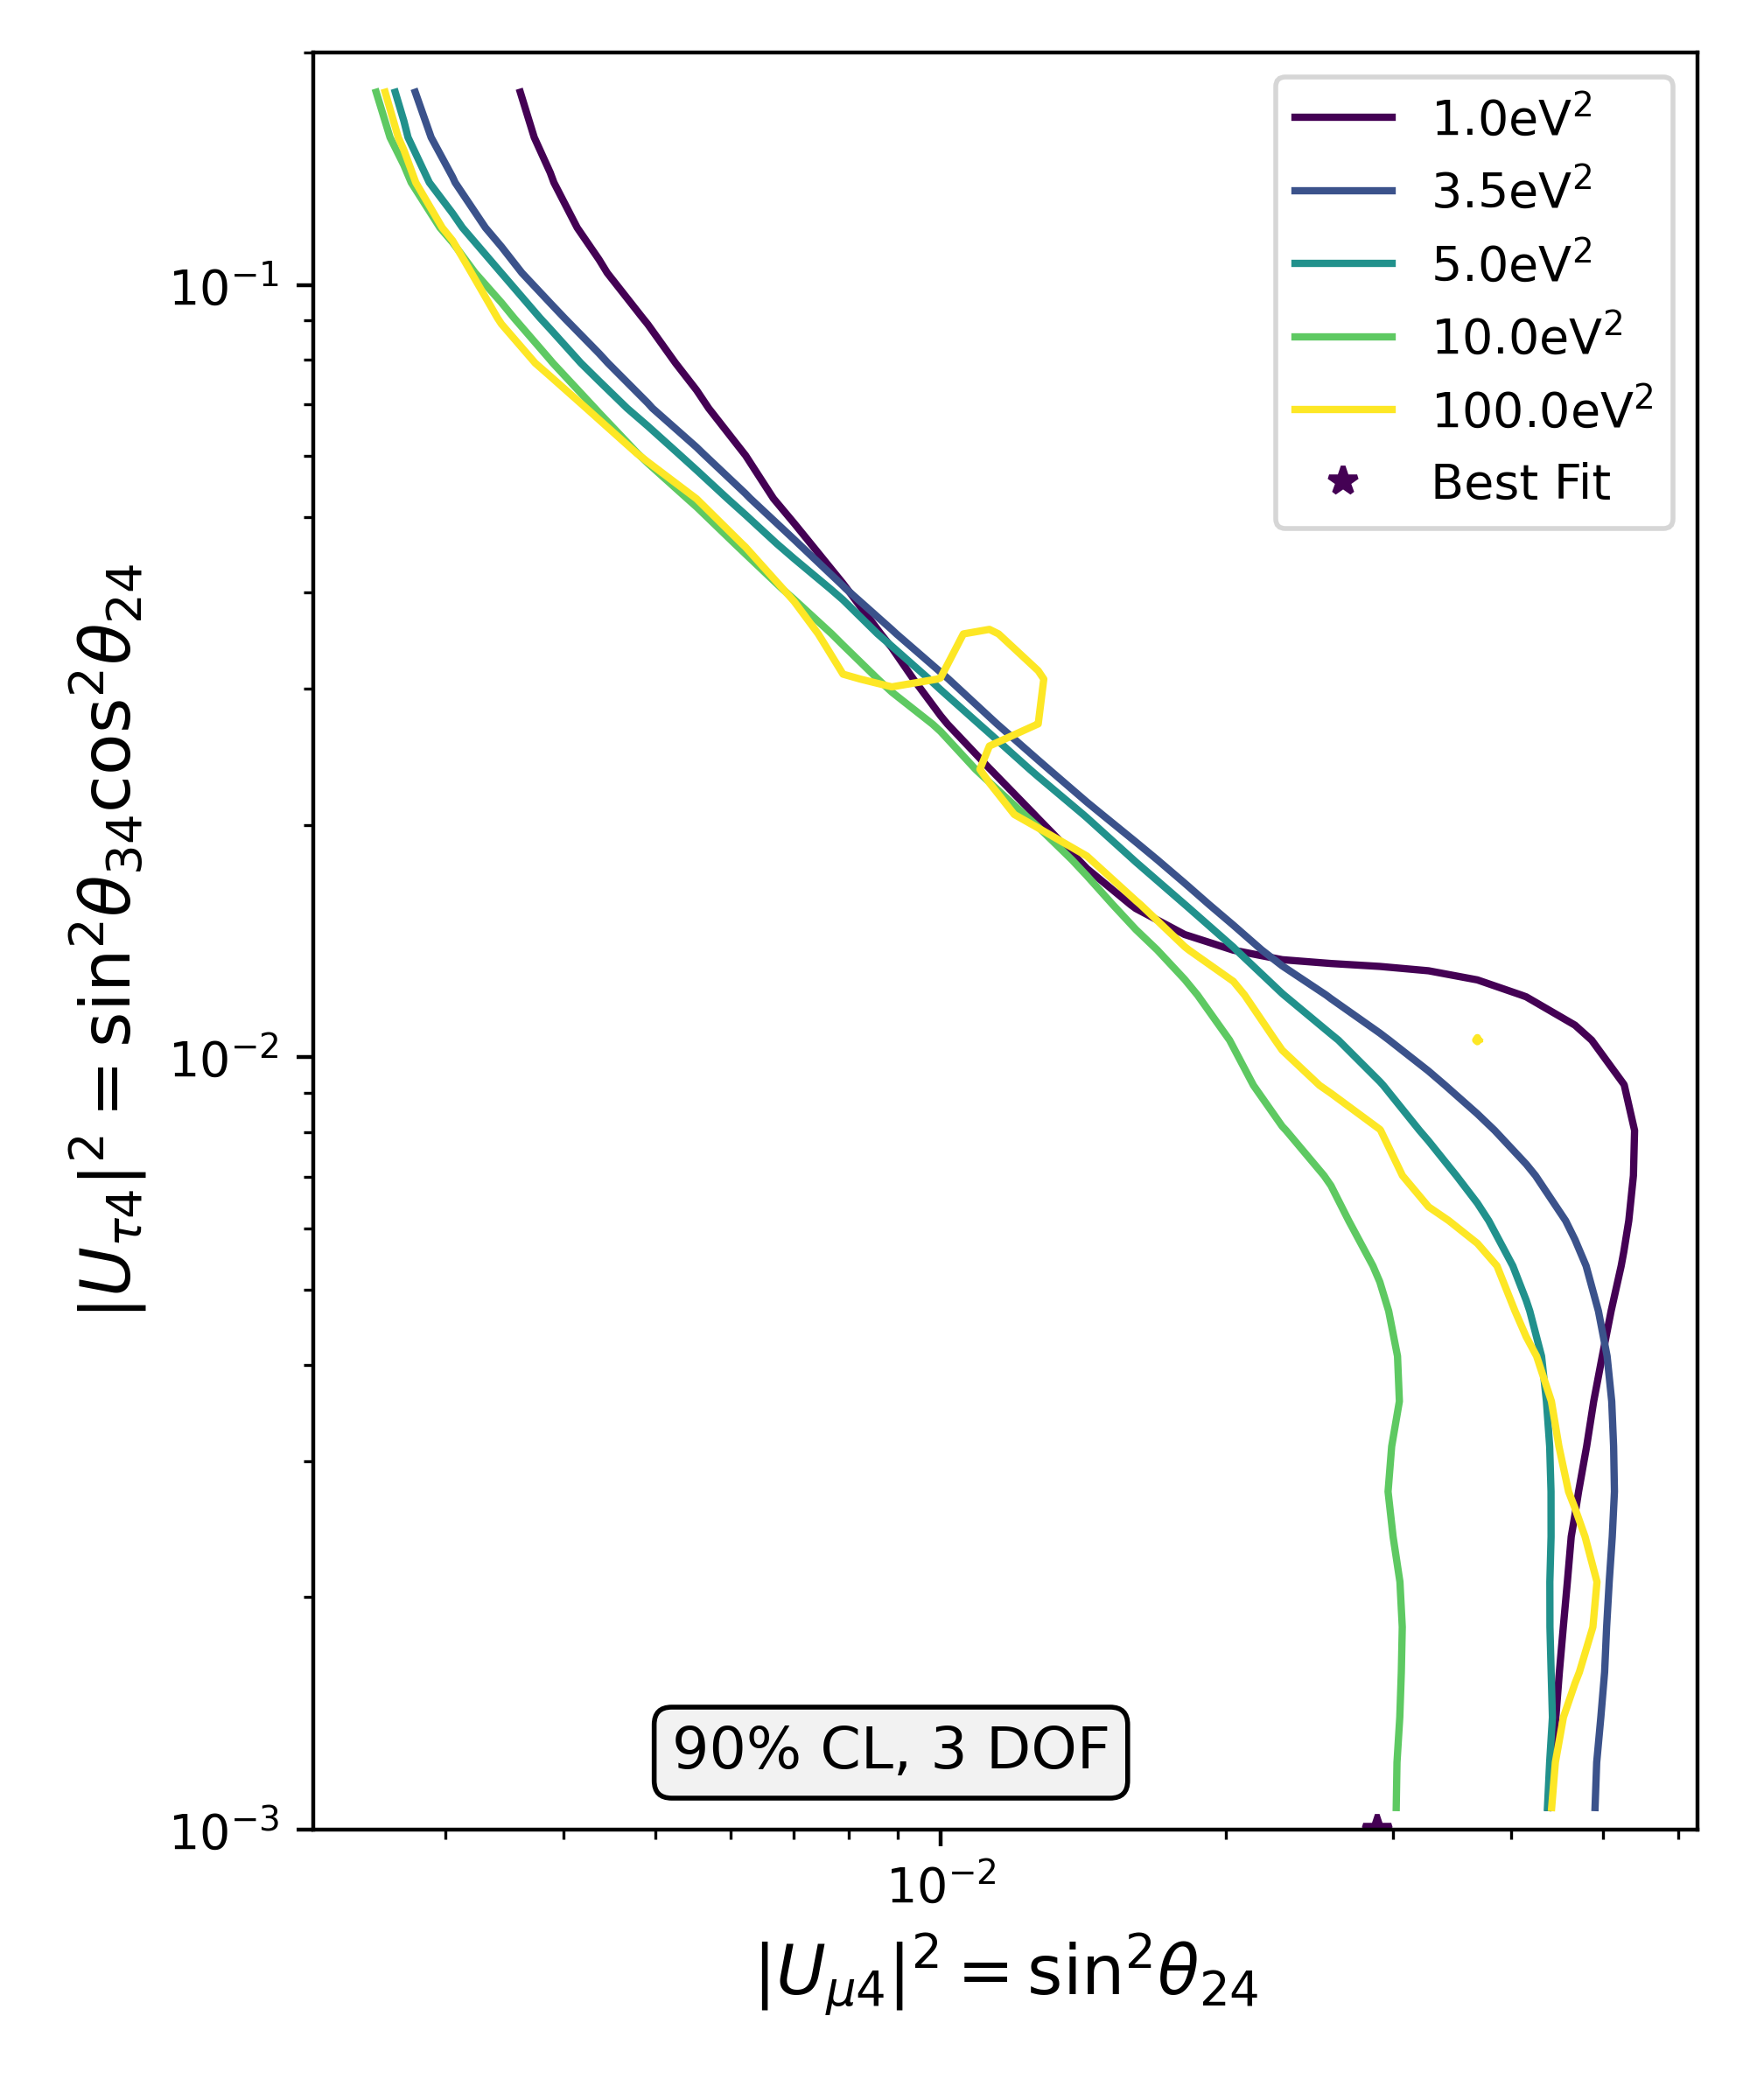
\includegraphics[width=0.425\linewidth]{figures/track_daemon_mismodel_nomeow_Realization_daemon_Asimov_sterile_0_cl0.9_dof3.png}
    \caption{Fit results after injecting daemonflux, but fitting assuming the flux model used in the IceCube 8-year sterile search. (Left) the 90\% CL contours for two degrees of freedom, $-2(\mathcal{L}_{best}-\mathcal{L}_{null})=5.02$ after fitting over $(\Delta m_{41}^{2}, \sin^{2}(2\theta_{24}))$, the results from the 8-year IceCube sterile search are overlain~\cite{Aartsen_2020, Aartsen_2020_prd}; (right) the 90\% CL contours for three degrees of freedom, $-2(\mathcal{L}_{best}-\mathcal{L}_{null})=4.7$ after fitting over $(\Delta m_{41}^{2}, \abs{U_{\mu4}}^{2}, \abs{U_{\tau 4}}^{2})$}\label{fig:uhoh_mismodel_worse}
\end{figure}

The converse was also investigated; fits were run assuming daemonflux, with its model of conventional flux uncertainty, while the conventional neutrino flux model used in the 8-year IceCube sterile search was injected as a true model. 
In this case, the best fit was consistent with a three-neutrino hypothesis, as shown in Figure~\ref{fig:daemon_midmodel}. 
This suggests that if the model used in the 8-year analysis is a better description of the truth, then assuming daemonflux is not likely to yield spurious signatures of 3+1 sterile neutrinos given no new physics. 

\begin{figure}  
    \centering
    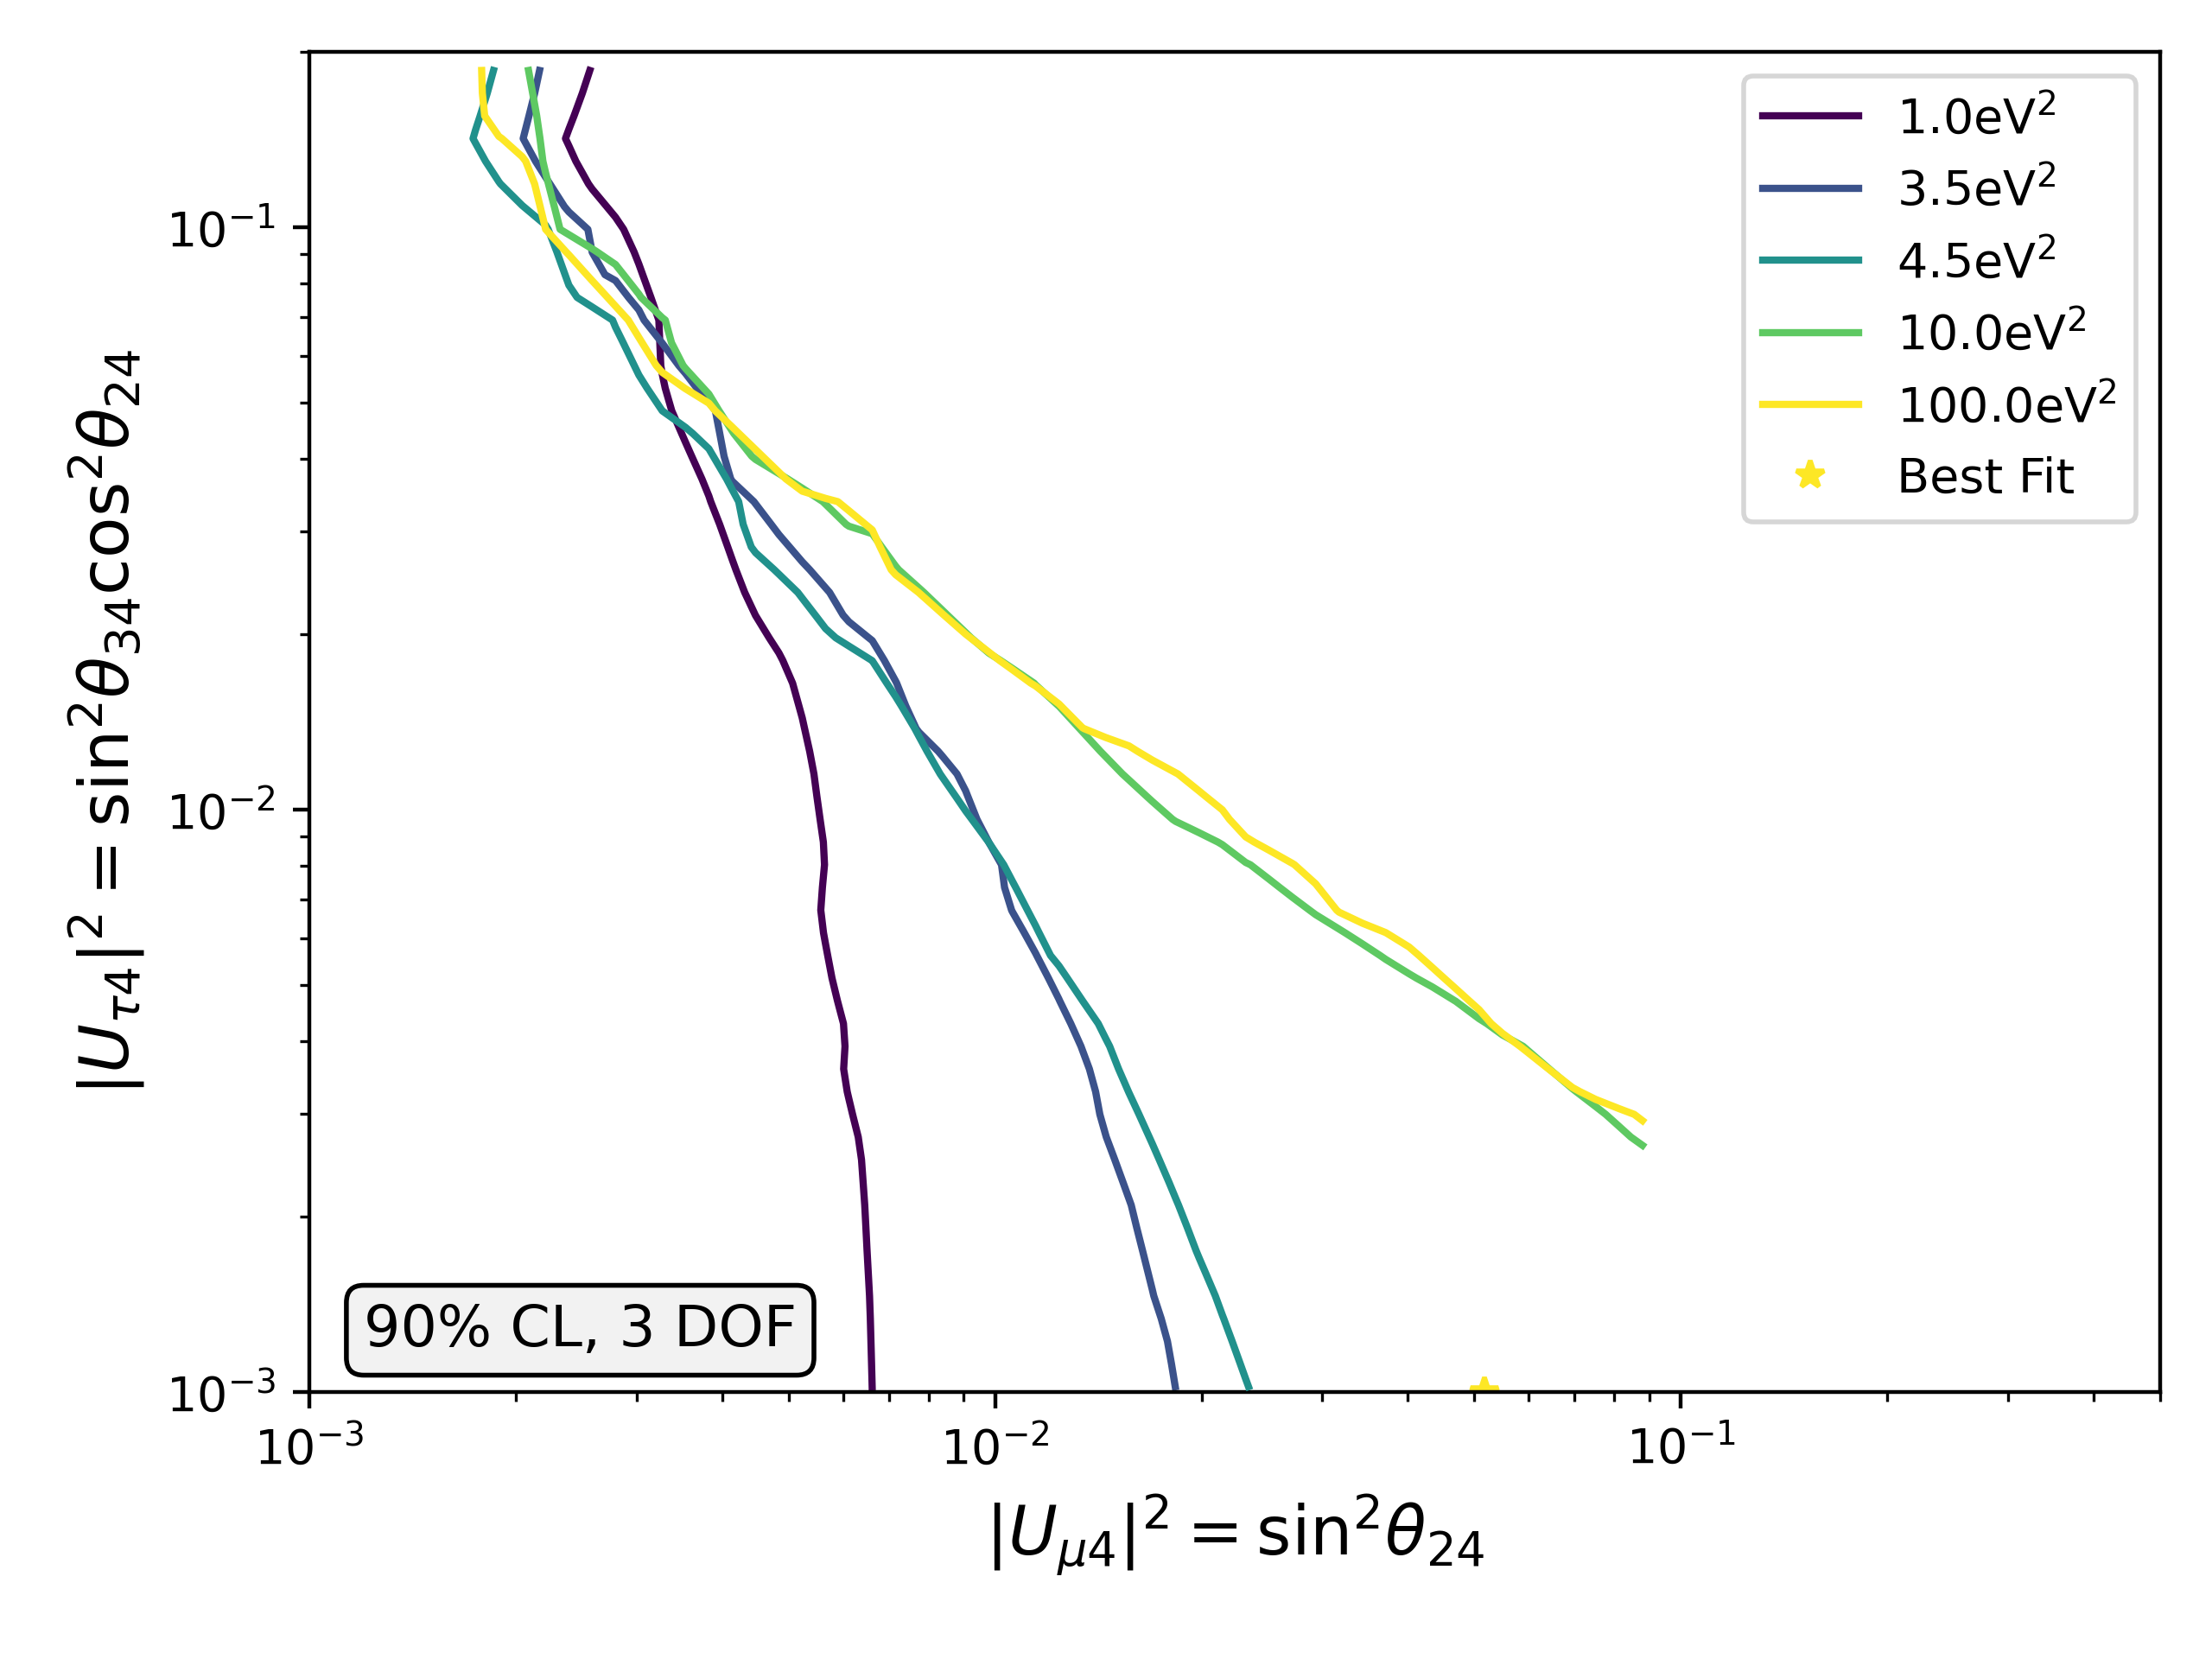
\includegraphics[width=0.7\linewidth]{figures/joint_daemon_inject_barr_Realization_Asimov_sterile_0_cl0.9_dof3.png}
    \caption{The 90\% CL contours for three degrees of freedom. A conventional flux model consistent with the 8-year IceCube sterile search is injected and daemonflux is assumed in fits. $-2(\mathcal{L}_{best}-\mathcal{L}_{null})=0.6$.}\label{fig:daemon_midmodel}
\end{figure}

Two additional checks were run. 
A neutrino flux prediction was made using the Global Spline Fit~\cite{dembinski2017datadriven}, the Sibyll2.3c interaction model~\cite{Riehn:2017mfm}, and the US Standard Atmospheric model~\cite{united1976u}. 
Fit scans were run on a pseudo-experimental result generated from this flux assuming (1) daemonflux and its uncertainties of the cosmic ray flux, and (2) the model used in the 8-year IceCube sterile search. 
These results are shown in Figure~\ref{fig:gsf_updates}. 
In both cases, no statistically significant signal is seen; each one is consistent with the injected null model. 

\begin{figure}  
    \centering
    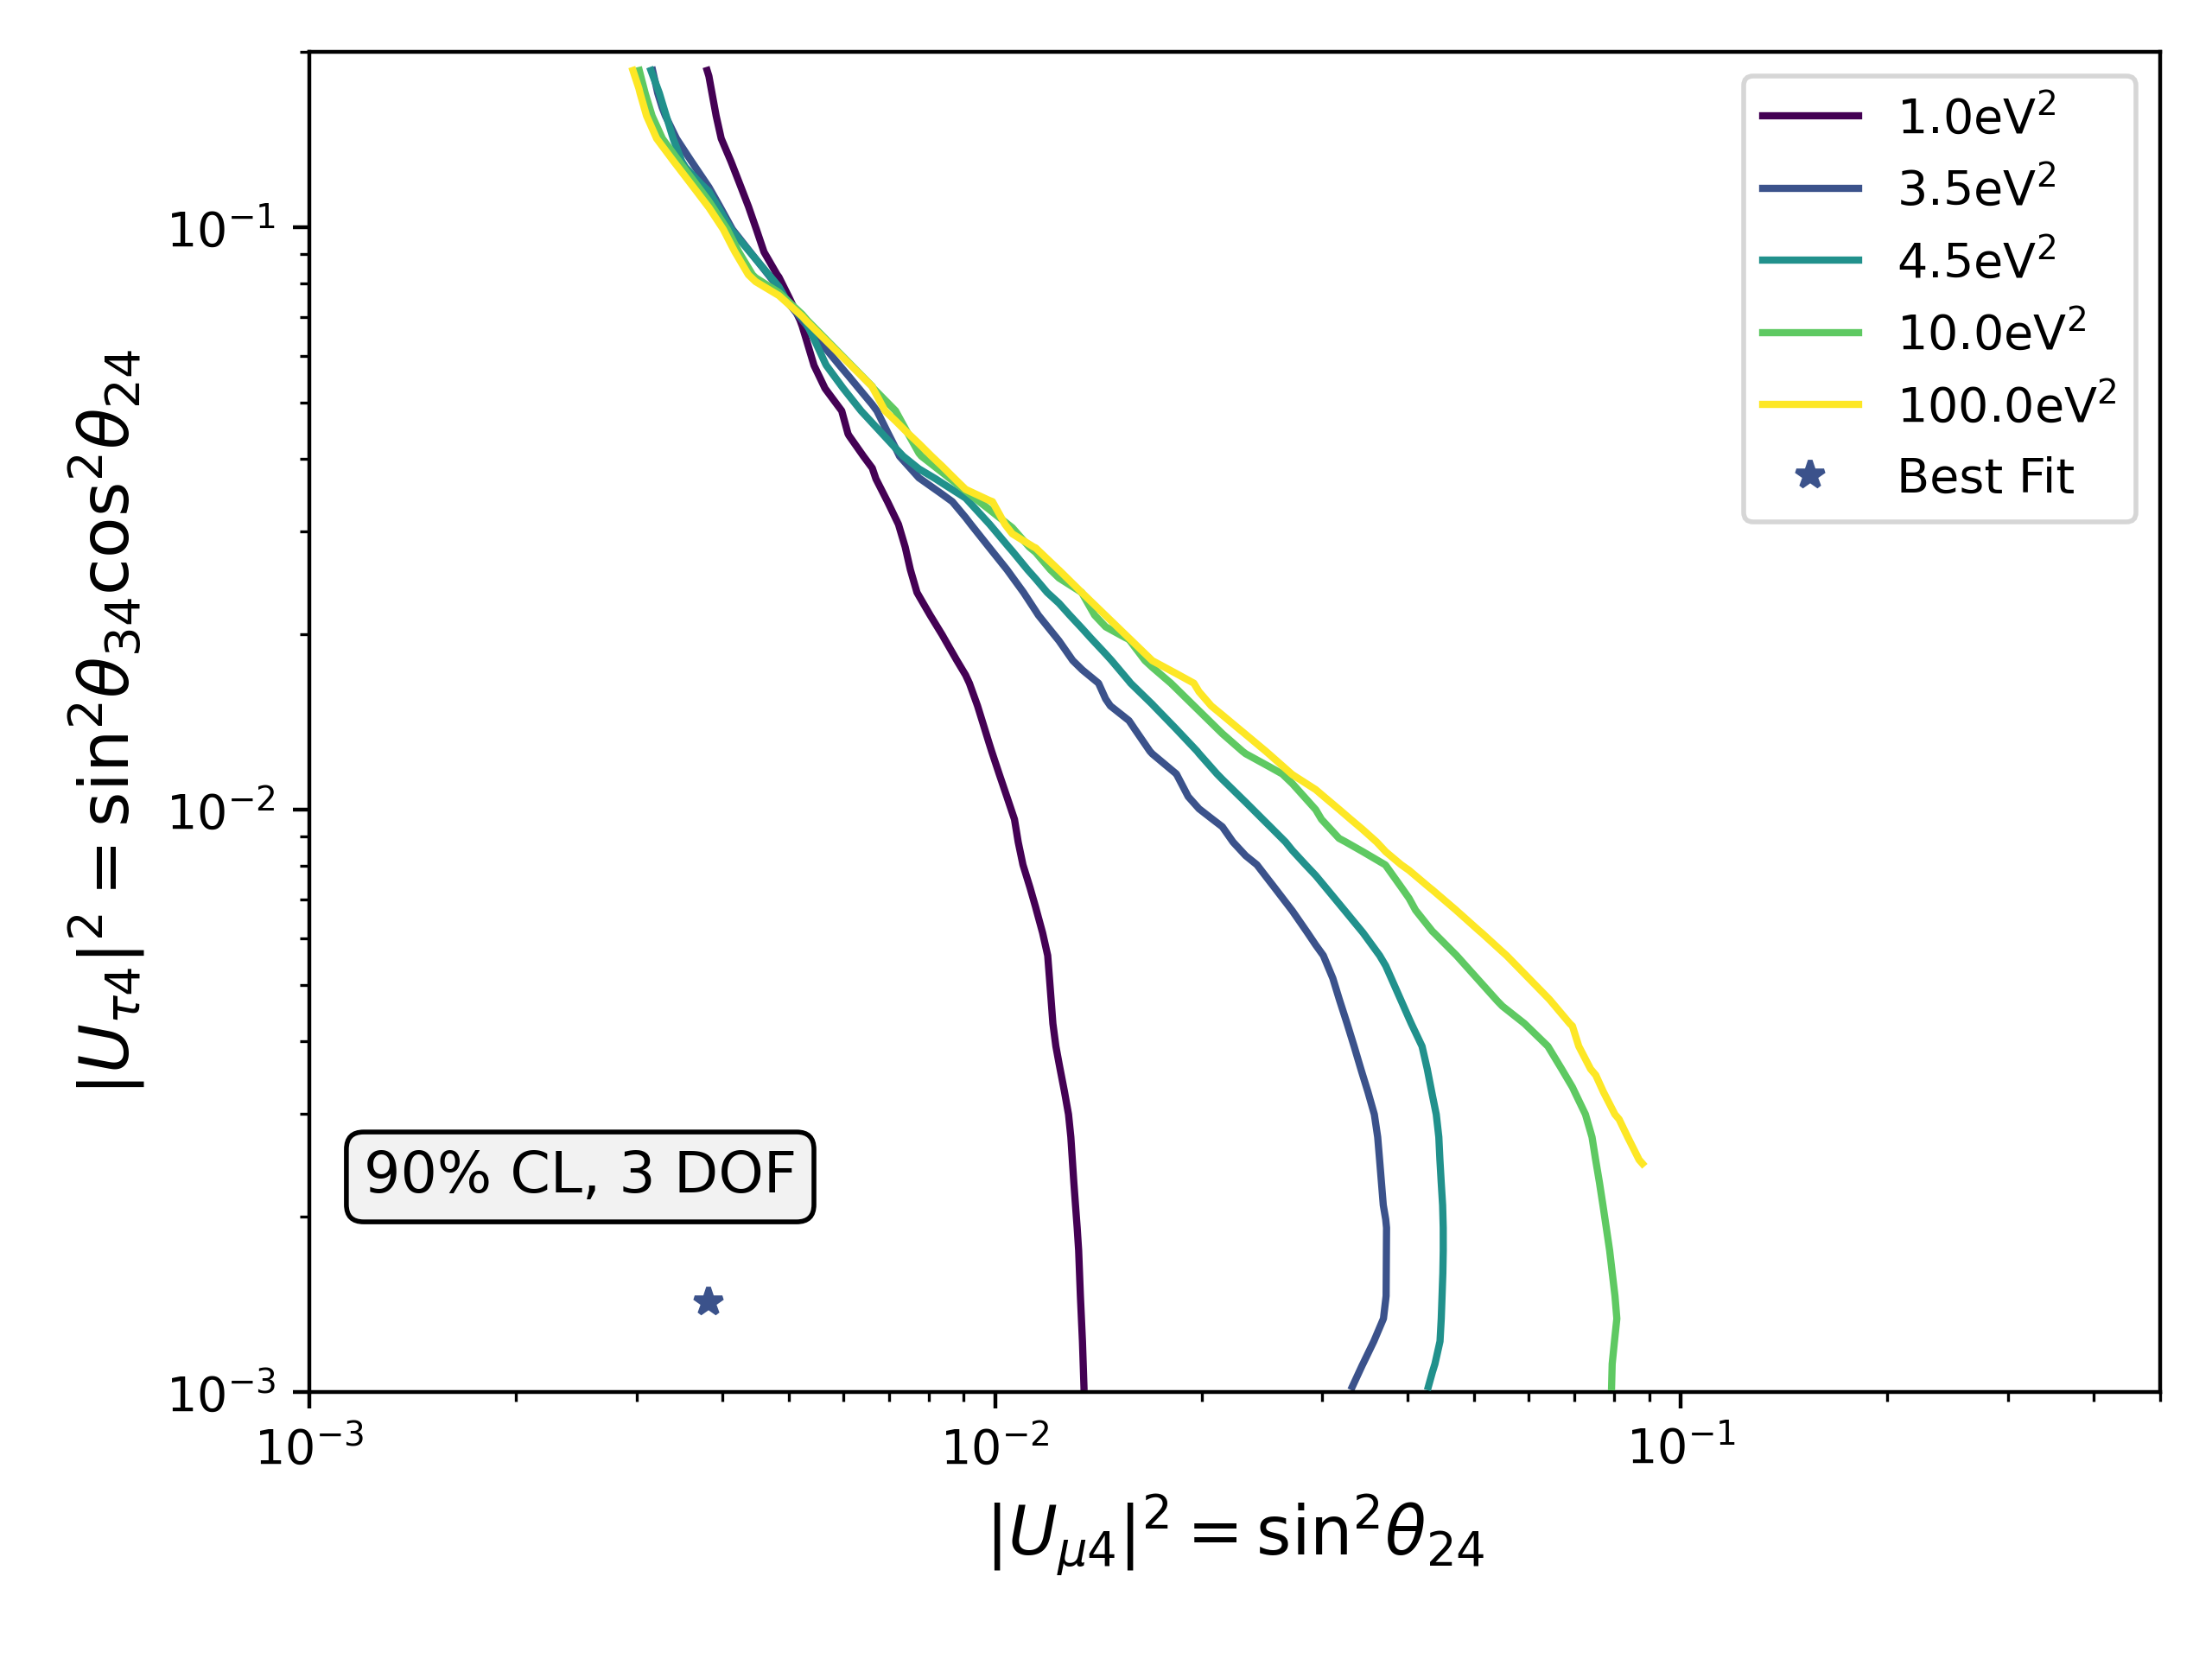
\includegraphics[width=0.45\linewidth]{figures/gsfinject_fitbarr_Realization_gsfdaemon_Asimov_sterile_0_cl0.9_dof3.png}
    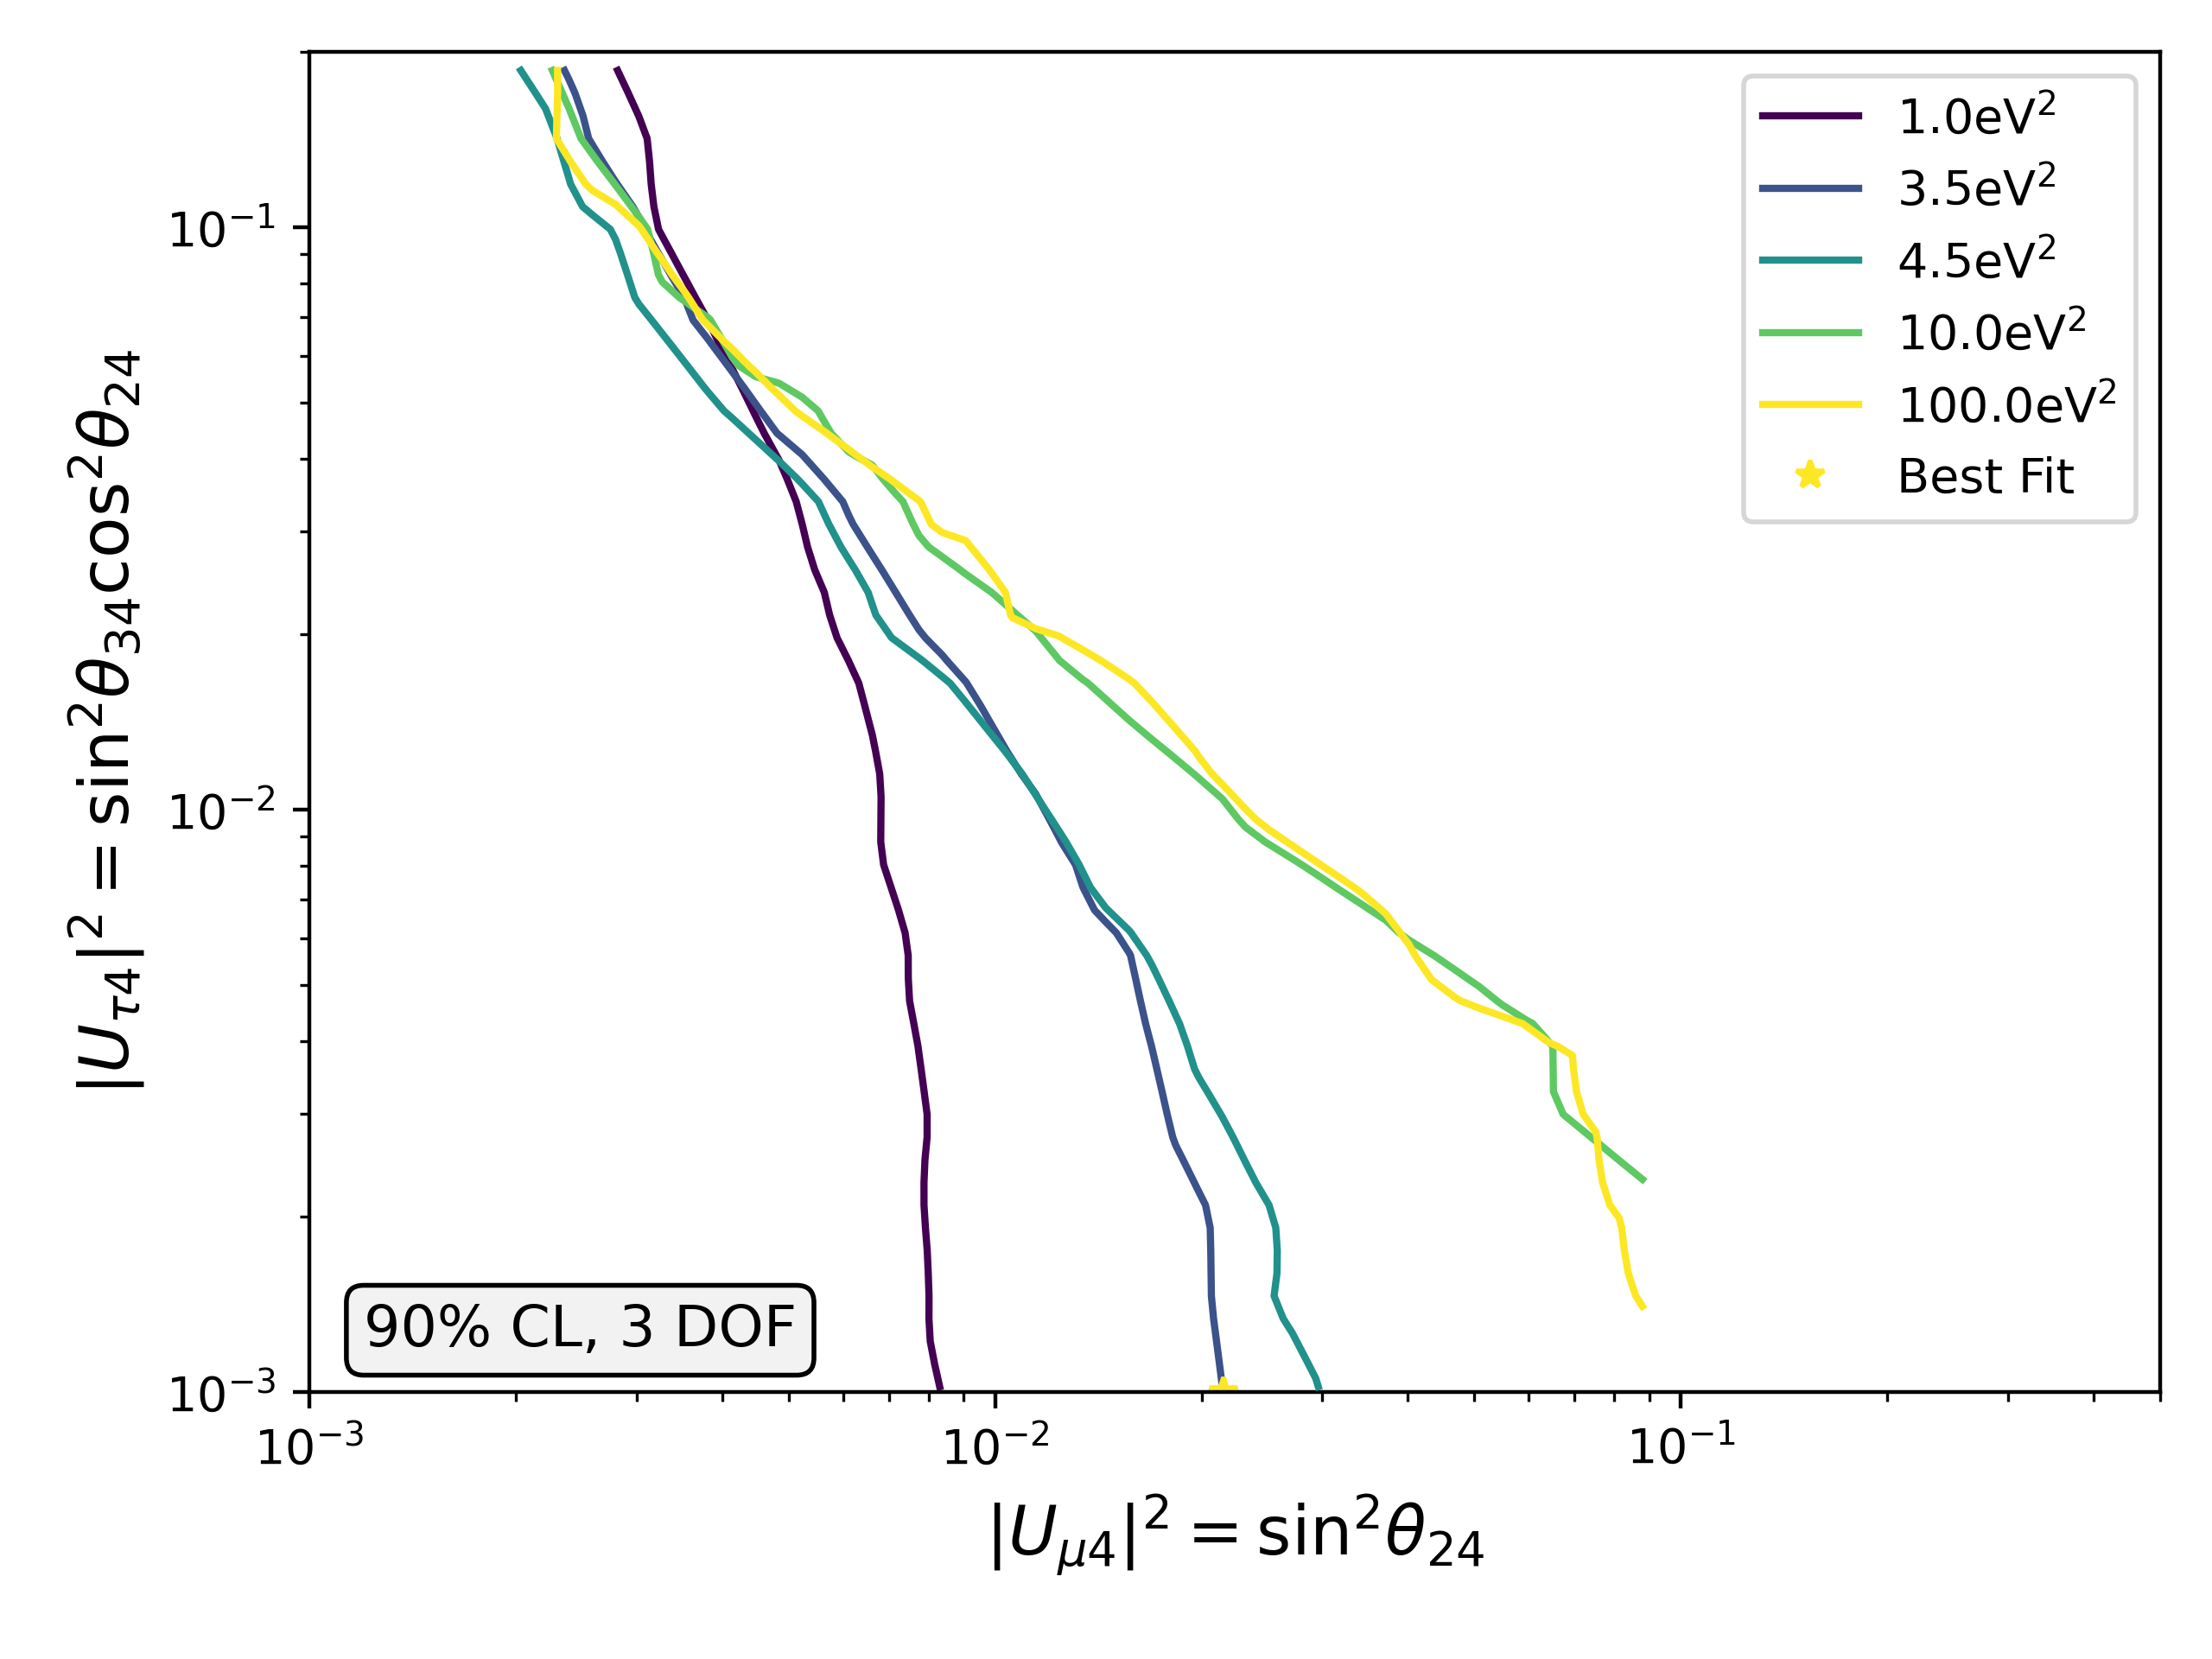
\includegraphics[width=0.45\linewidth]{figures/gsfinject_fitdaemon_Realization_gsfdaemon_Asimov_sterile_0_cl0.9_dof3.png}
    \caption{On the left (right), fit results after injecting the new GSF model while assuming the model used in the 8-year IceCube sterile search (daemonflux), $-2(\mathcal{L}_{best}-\mathcal{L}_{null})=0.6$ $(0.2)$.}\label{fig:gsf_updates}
\end{figure}

In order to minimize the possibility that our choice of conventional neutrino flux model could bias a measurement of sterile neutrino oscillations, or yield a spurious signal, we opted to fully adopt daemonflux as our nominal flux model and as our description of conventional flux uncertainties. 

\subsection{Astrophysical Mismodeling}

Recently, the IceCube Neutrino Observatory became the first experiment to observe an excess of astrophysical neutrinos coming from the Milky Way\cite{doi:10.1126/science.adc9818}. 
This extra population of neutrinos is produced from cosmic-ray interactions with the interstellar medium throughout our galaxy: causing the Milky Way to glow with neutrinos. 
In this, and similar oscillations analyses, the astrophysical neutrino flux has been assumed to be isotropic. 
A test was carried out where a non-isotropic flux modeling the Milky Way, the KRA$\gamma$-50~\cite{Gaggero_2015} model, is injected in addition to an isotropic flux but with no new physics signatures. 
A fit scan is then ran assuming an isotropic flux and the resulting likelihood profile is found. 
The exclusion contours, with best fit, are shown in Figure~\ref{fig:galaxy}.
No spurious preference for new physics is seen, and so we conclude that any anisotropic excess in the astrophysical neutrino flux will not bias this analysis' result. 

\begin{figure}
    \centering
    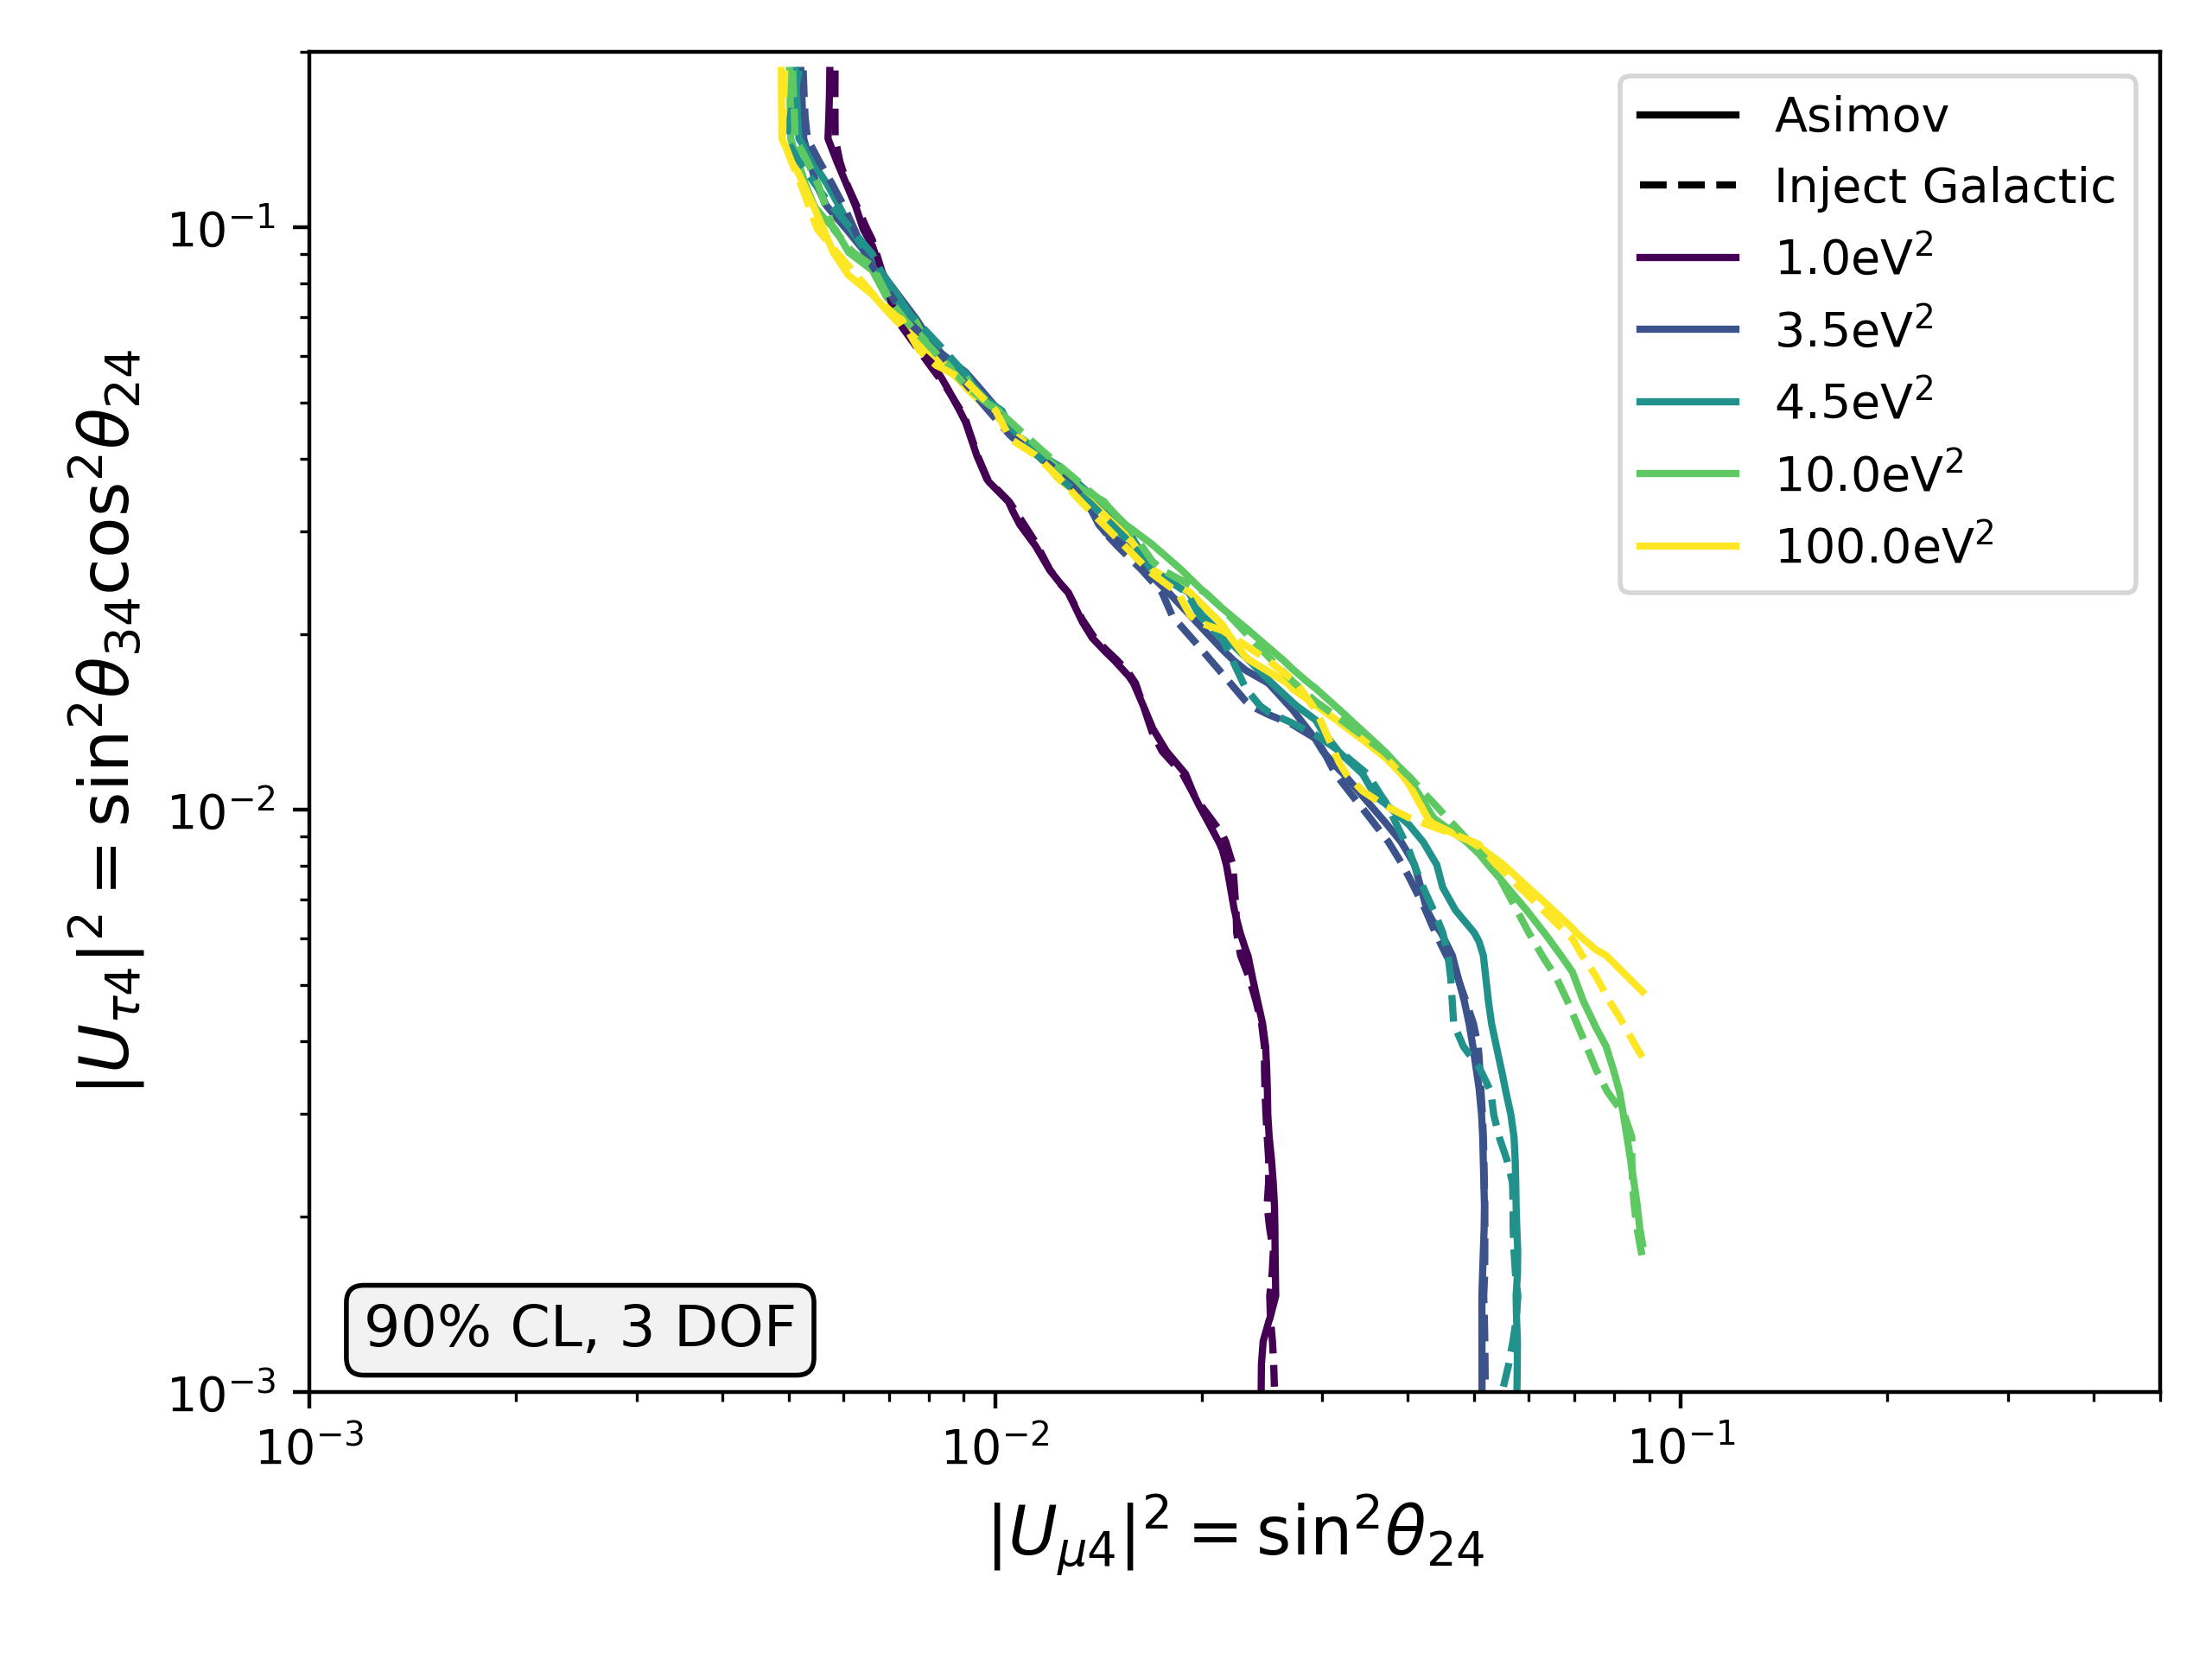
\includegraphics[width=0.7\linewidth]{figures/double_galactic_mismodel_fix_Realization_galactic_focus_sterile_0_cl0.9_dof3.png}
    \caption{Exclusion contours at 90\% CL and for three degrees of freedom for an Asimov realization (solid) and a KRA$\gamma$-50 injected neutrino flux (dashed). The contours have considerable overlap and no spurious 3+1 signatures are observed}\label{fig:galaxy}
\end{figure}

\subsection{Astrophysical Flavor Mismodeling}

Since the chosen prior does not span the full range of astrophysical flavor ratios allowed at $3\sigma$, a flavor-ratio mismodeling test was carried out.
A pseudo-experimental result was generated assuming a flavor ratio ($f_{e}:f_{\mu}:f_{\tau}$) of (0.35,0.2,0.45); an allowed value that is not spanned by the astrophysical nuisance parameter. 
A fit-scan was then carried out injecting the above as the truth, and the resulting 90\% CL contours are shown in Figure~\ref{fig:flavor_mismodel}. The nuisance parameter pulls at the best fit are also shown in Figure~\ref{fig:flavor_mismodel_pulls}.
As can be seen, the flavor ratio pulls down to match the injected flavor ratio, and no spurious new physics signature is seen. 
From this we can conclude that the analysis-level representation of flavor space is sufficiently spanned by this nuisance parameter, and that a true flavor ratio not explicitly accessible will not bias our results. 

\begin{figure}
    \centering
    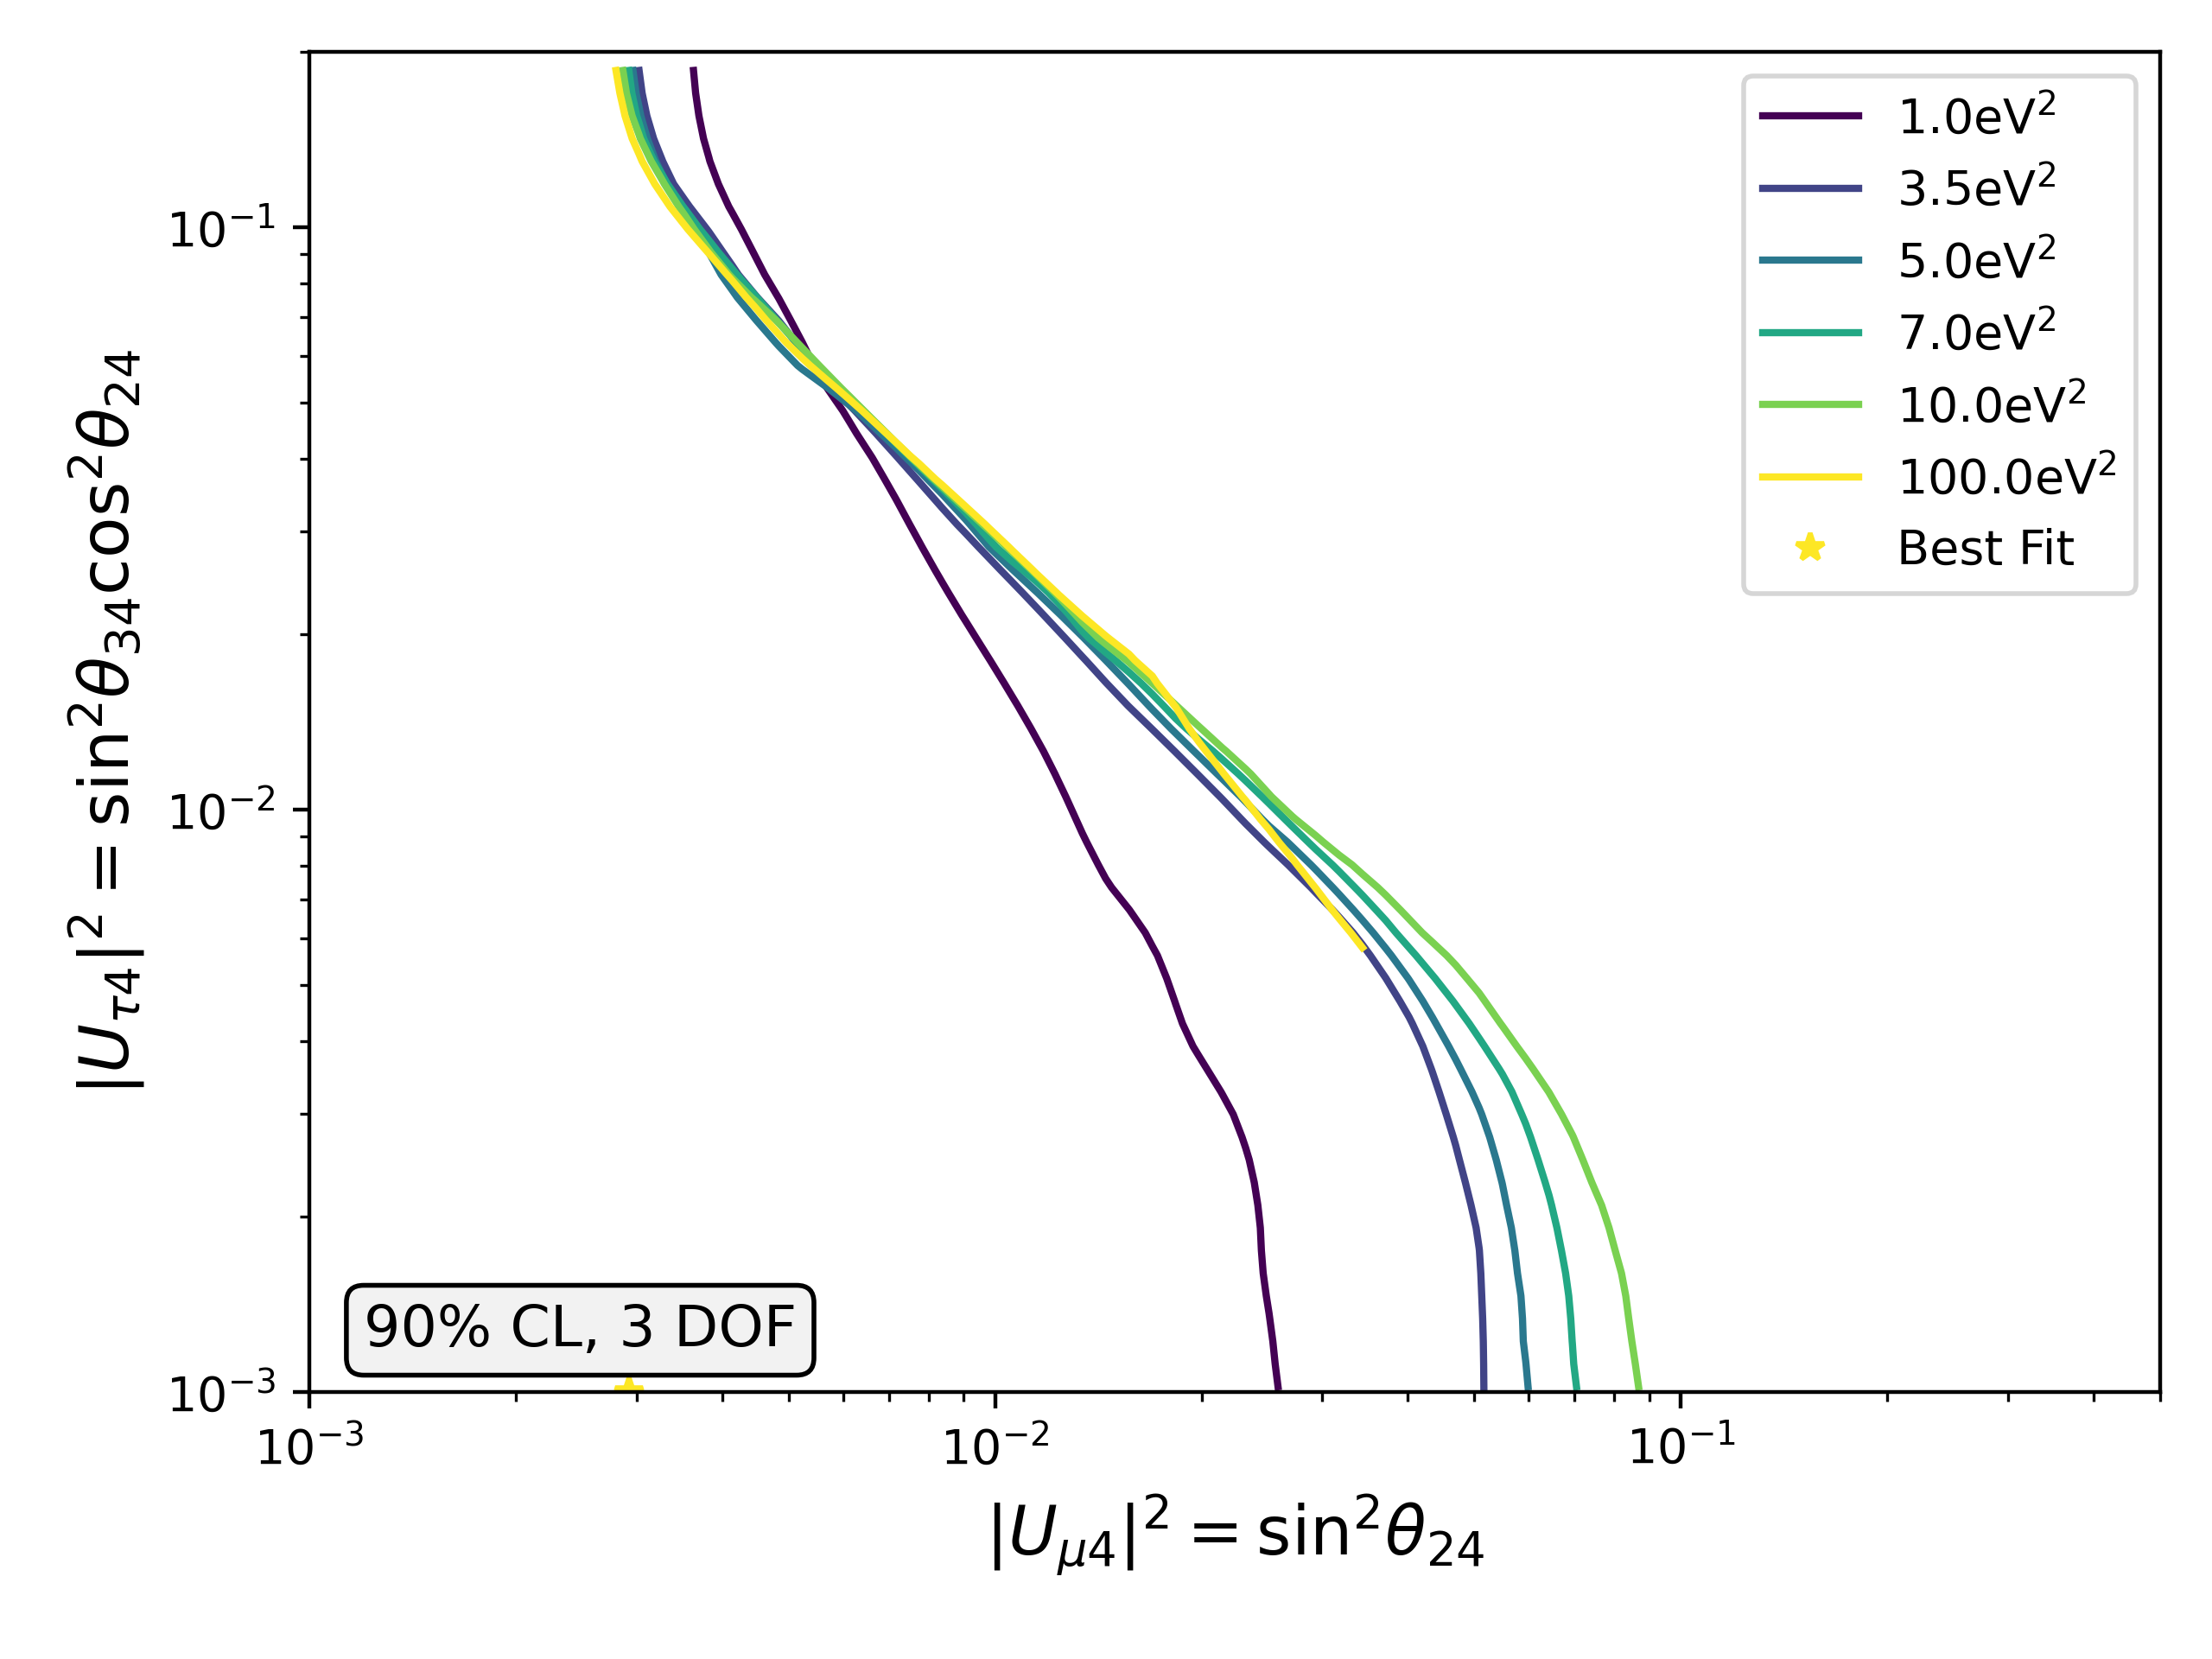
\includegraphics[width=0.7\linewidth]{figures/joint_astro_flavor_misfit_Realization_daemon_badflavor_Asimov_sterile_0_cl0.9_dof3.png}
    \caption{Exclusion contours at 90\% CL and for three degrees of freedom while injecting an astrophysical flavor ratio outside the values spanned by the nuisance parameters.}\label{fig:flavor_mismodel}
\end{figure}

\begin{figure}
    \centering
    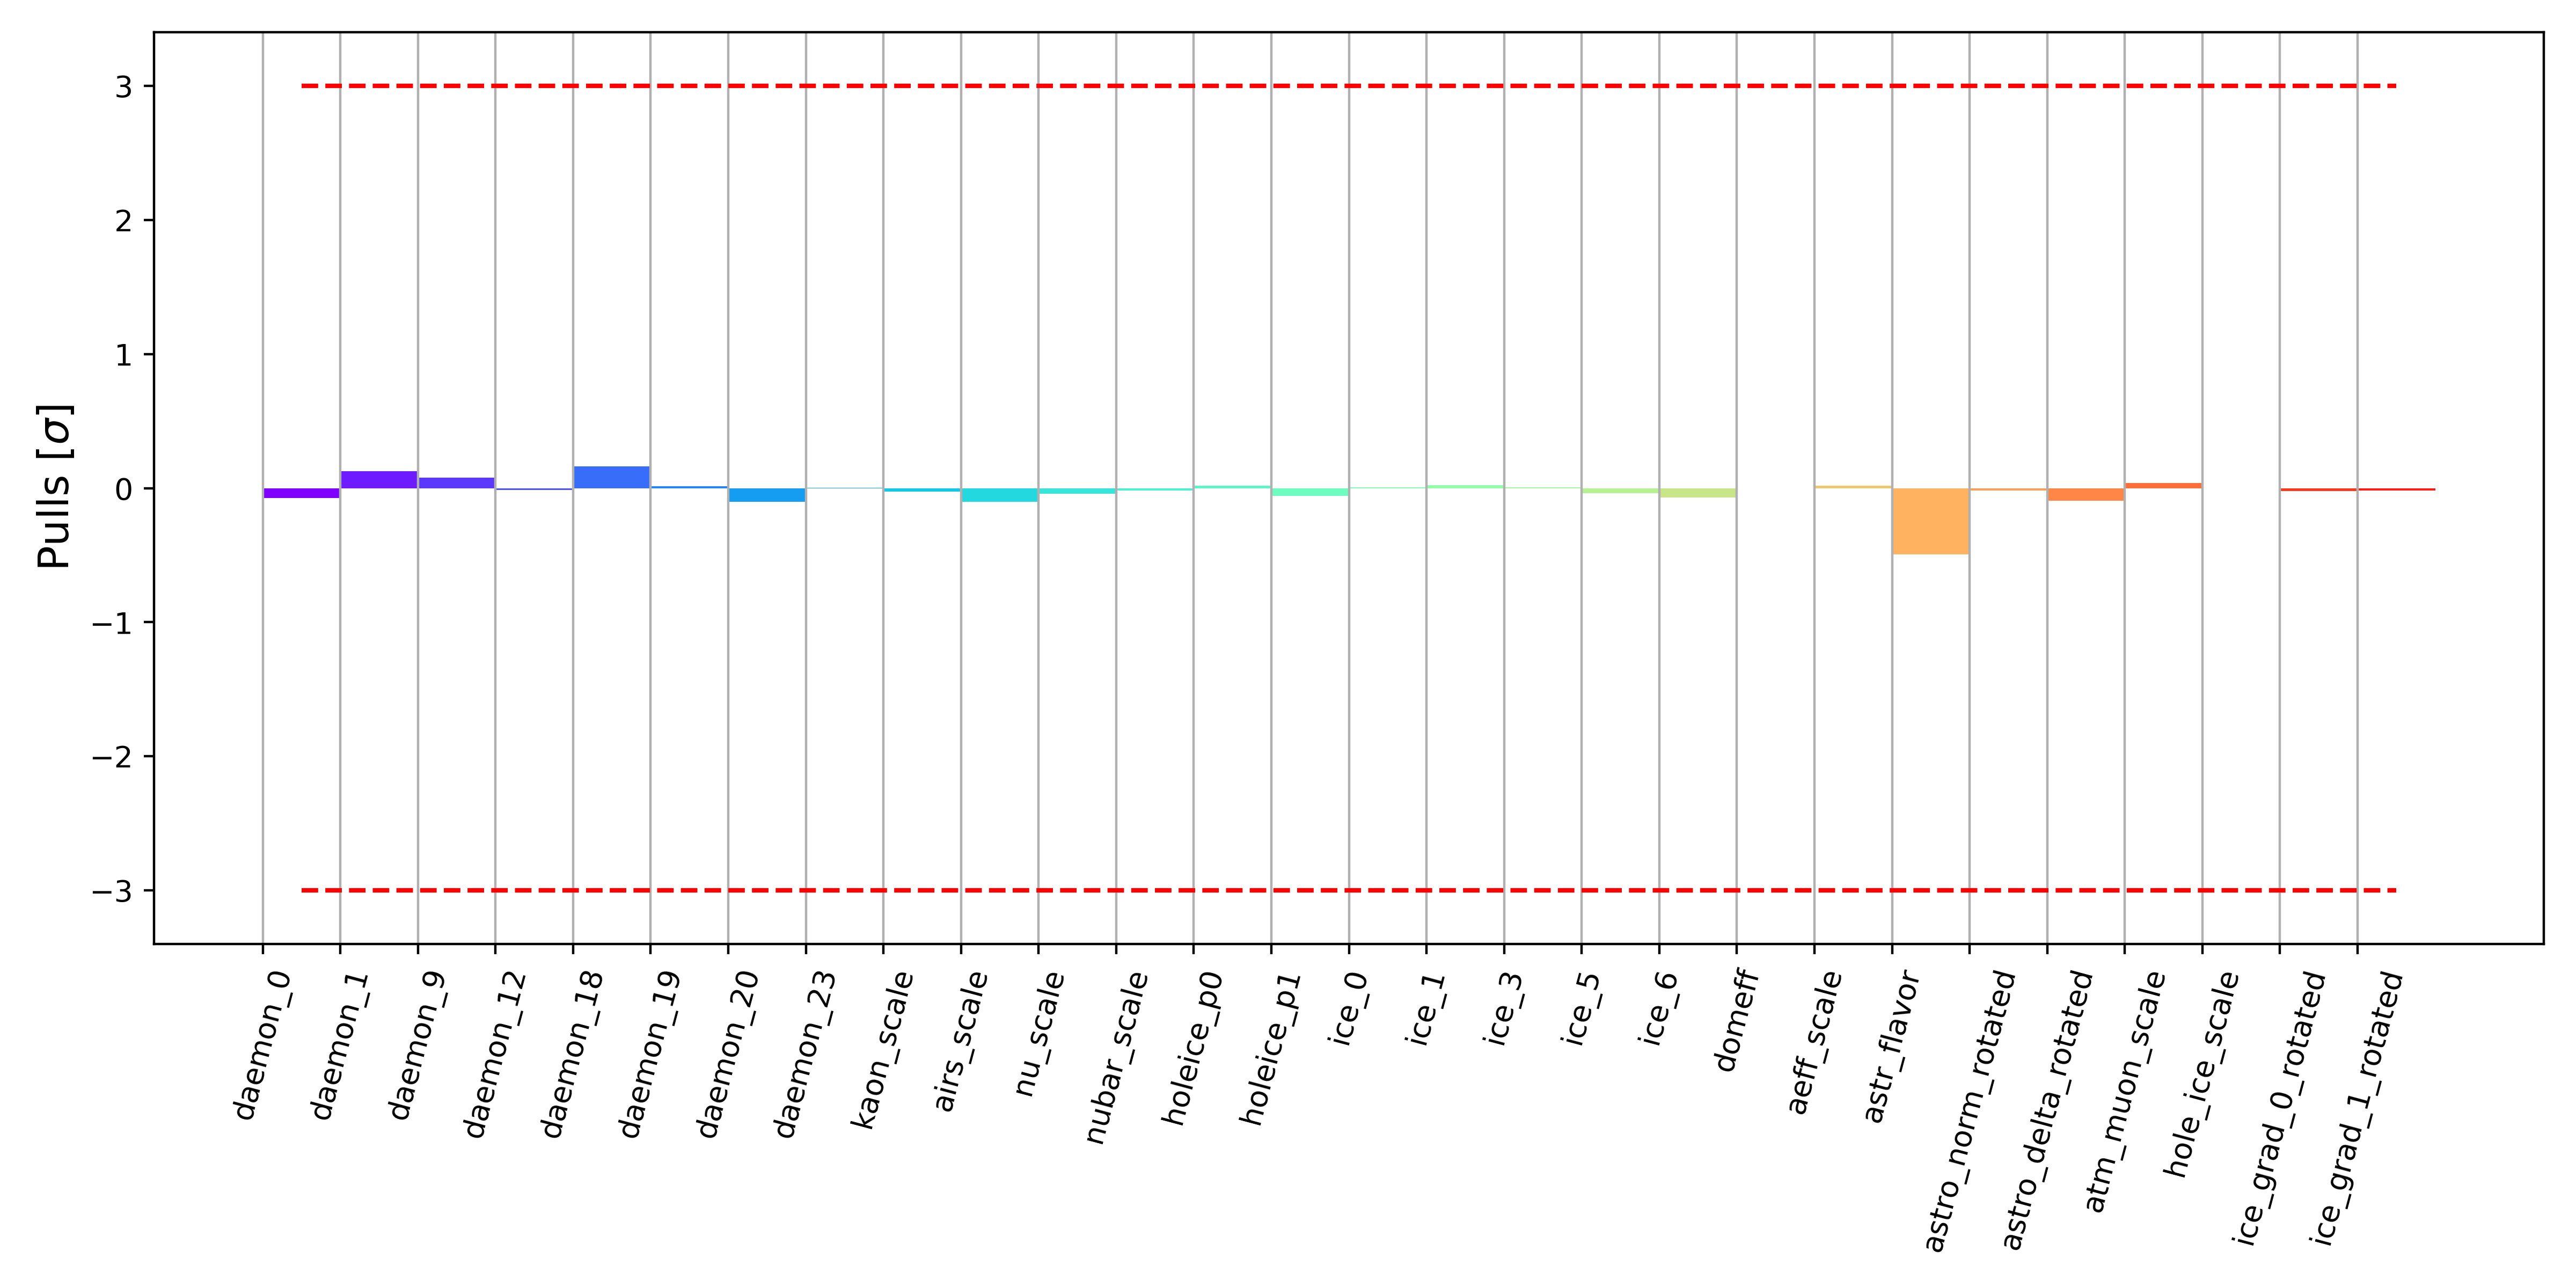
\includegraphics[width=0.7\linewidth]{figures/pulls_Realization_daemon_badflavor_Asimov_sterile_0_joint_astro_flavor_misfit.png}
    \caption{The pulls at the best fit point in the fit-scan shown in Figure~\ref{fig:flavor_mismodel}.}\label{fig:flavor_mismodel_pulls}
\end{figure}

\subsection{CR Muon Mismodeling}

As discussed earlier in Section~\ref{sec:cr_muon}, the cosmic ray muon background is considerable for the cascades sub-sample. 
In addition to those methods in-place to account for its contributions, a few tests were run to check if under-predicting the CR muons could mimic a 3+1 sterile neutrino signature. 
To this end, fit-scans were run under different situations:
\begin{enumerate}[label=(\alph*)]
    \item A normal amount of CR muons are injected, but none are assumed, with no MC statistical error 
    \item double the expected CR muons are injected, but the normal amount is assumed 
    \item double the expected CR muons are injected, but none are assumed and with no additional MC statistical error 
\end{enumerate}
The resulting contours are shown in Figures~\ref{fig:first_muon_sad} through~\ref{fig:last_muon_sad} below. 
No spurious 3+1 sterile signature was seen in any of these tested cases, and so we can conclude that any reasonable cosmic ray muon fluxes beyond our nominal expectation will not bias this analysis significantly.

\begin{figure}
    \centering
    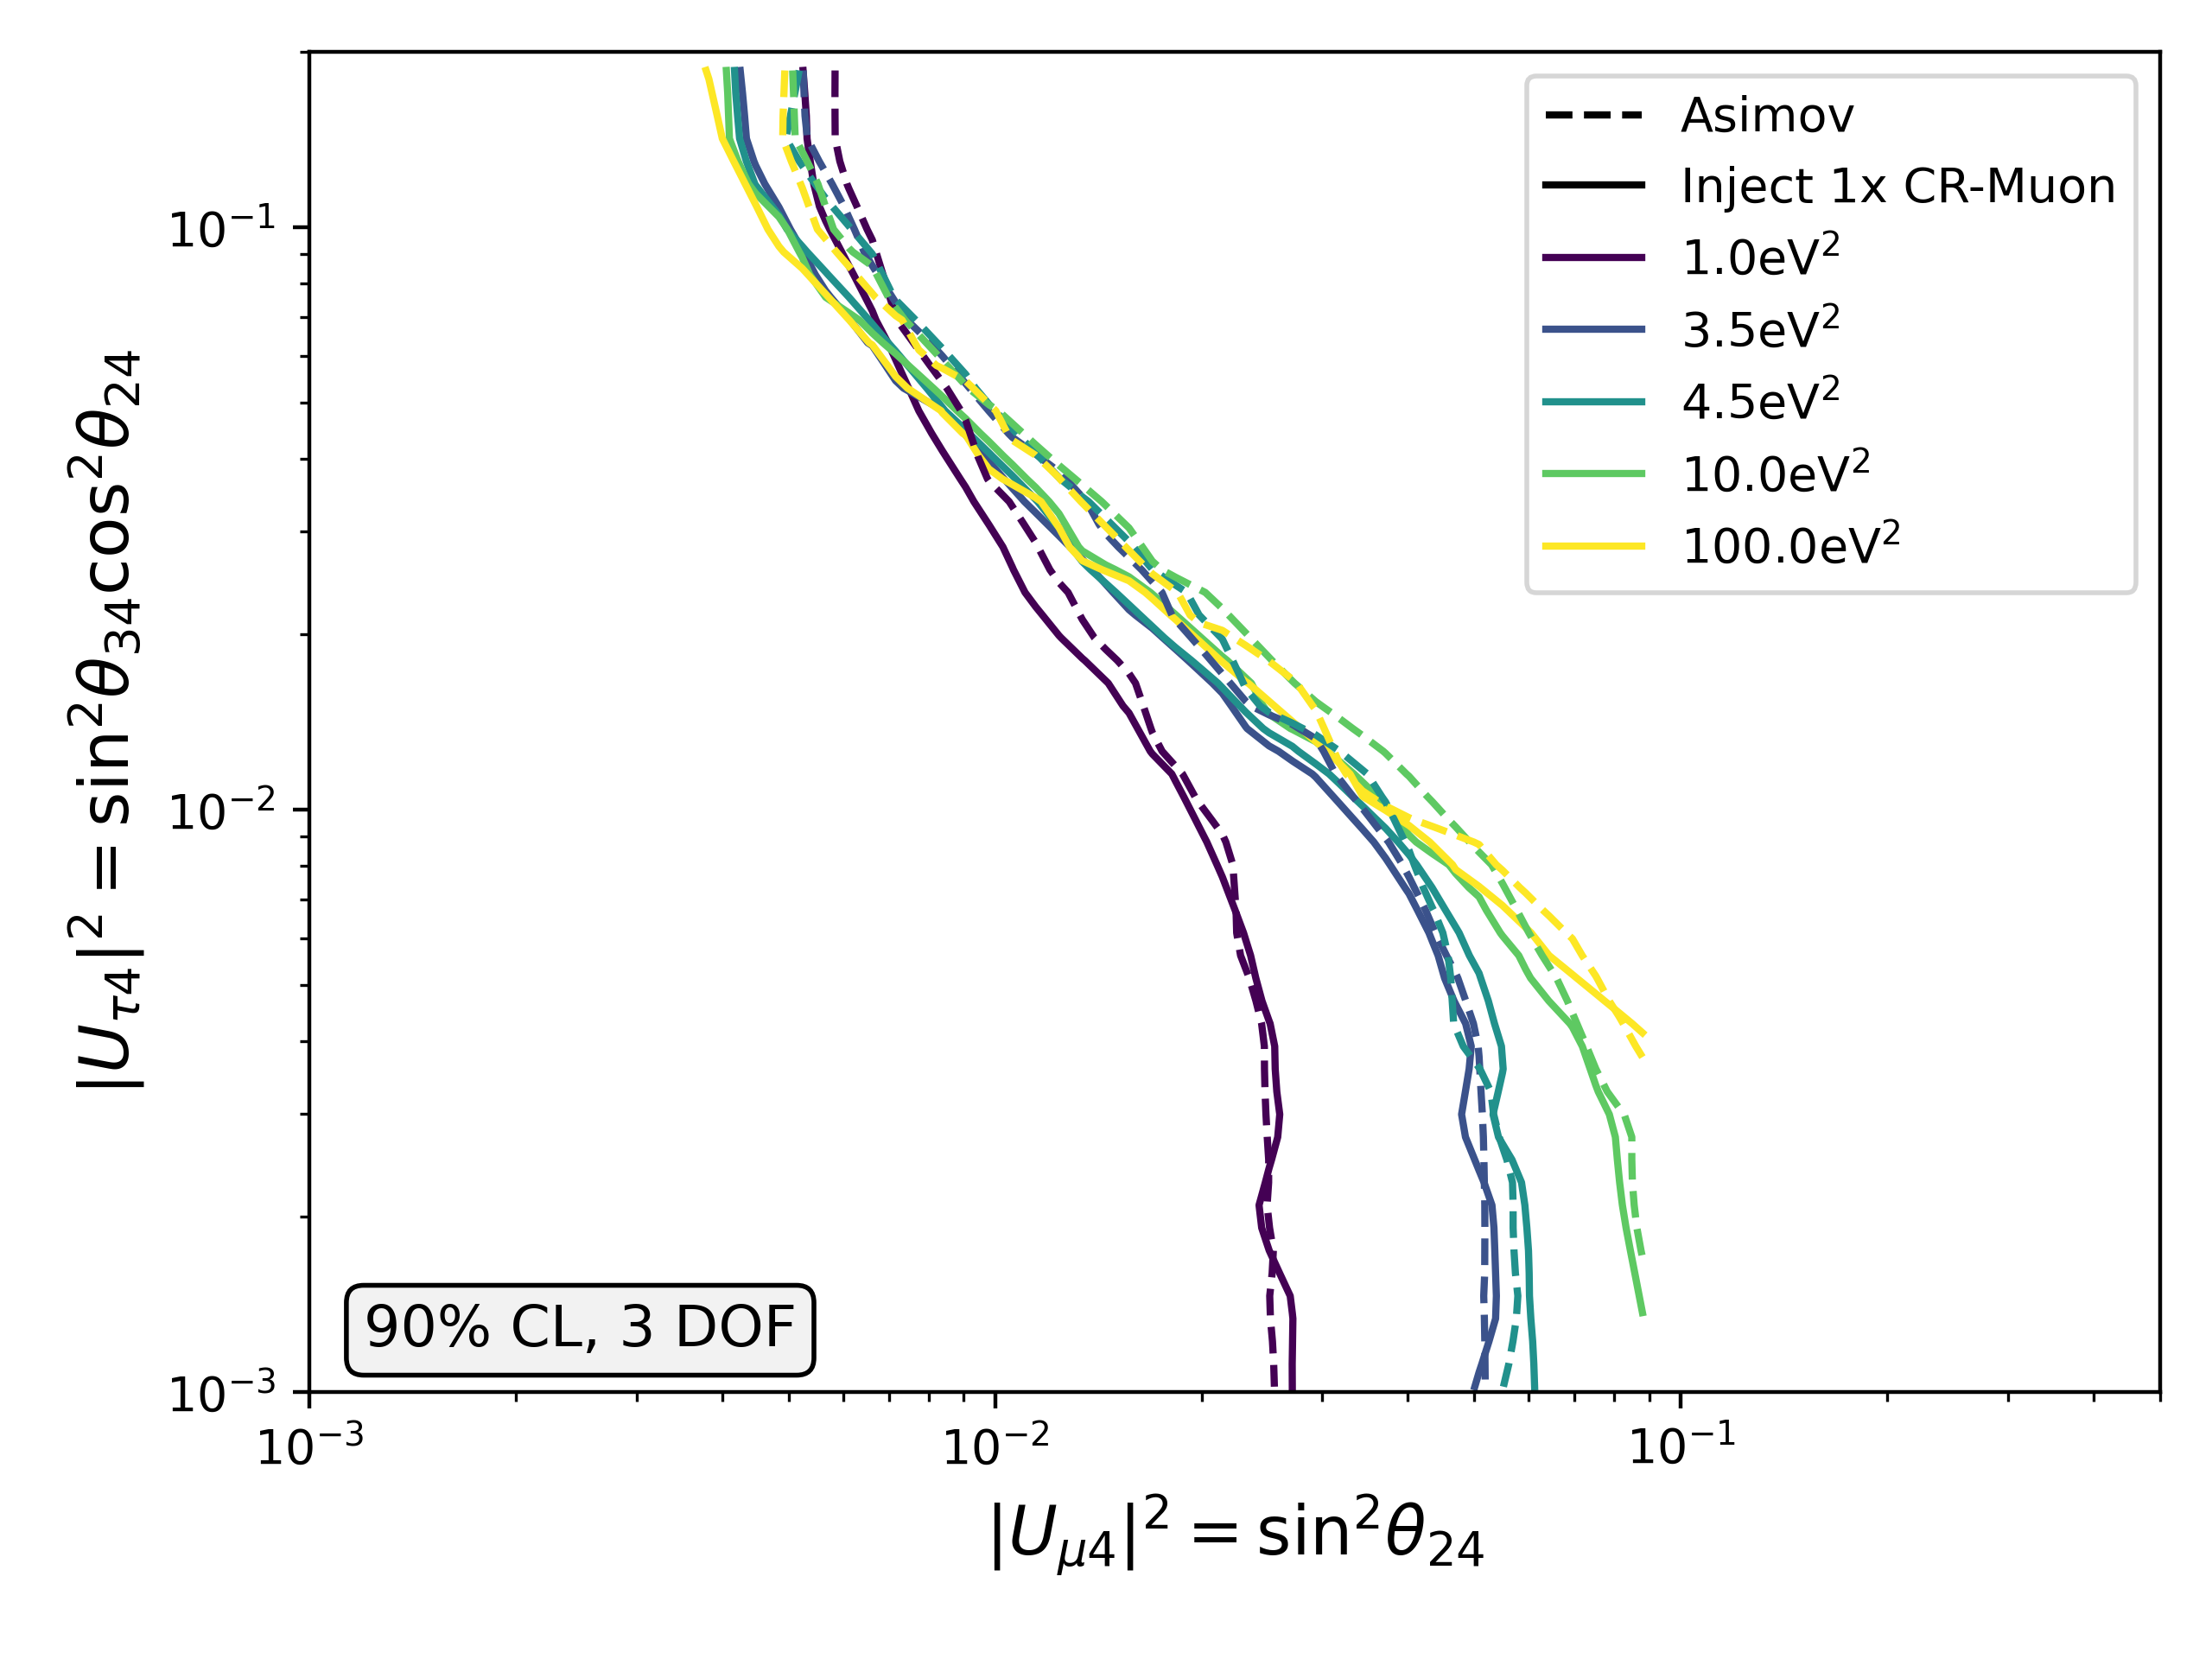
\includegraphics[width=0.45\linewidth]{figures/double_muon_mismodel_worse_Realization_Asimov_sterile_0_cl0.9_dof3.png}
    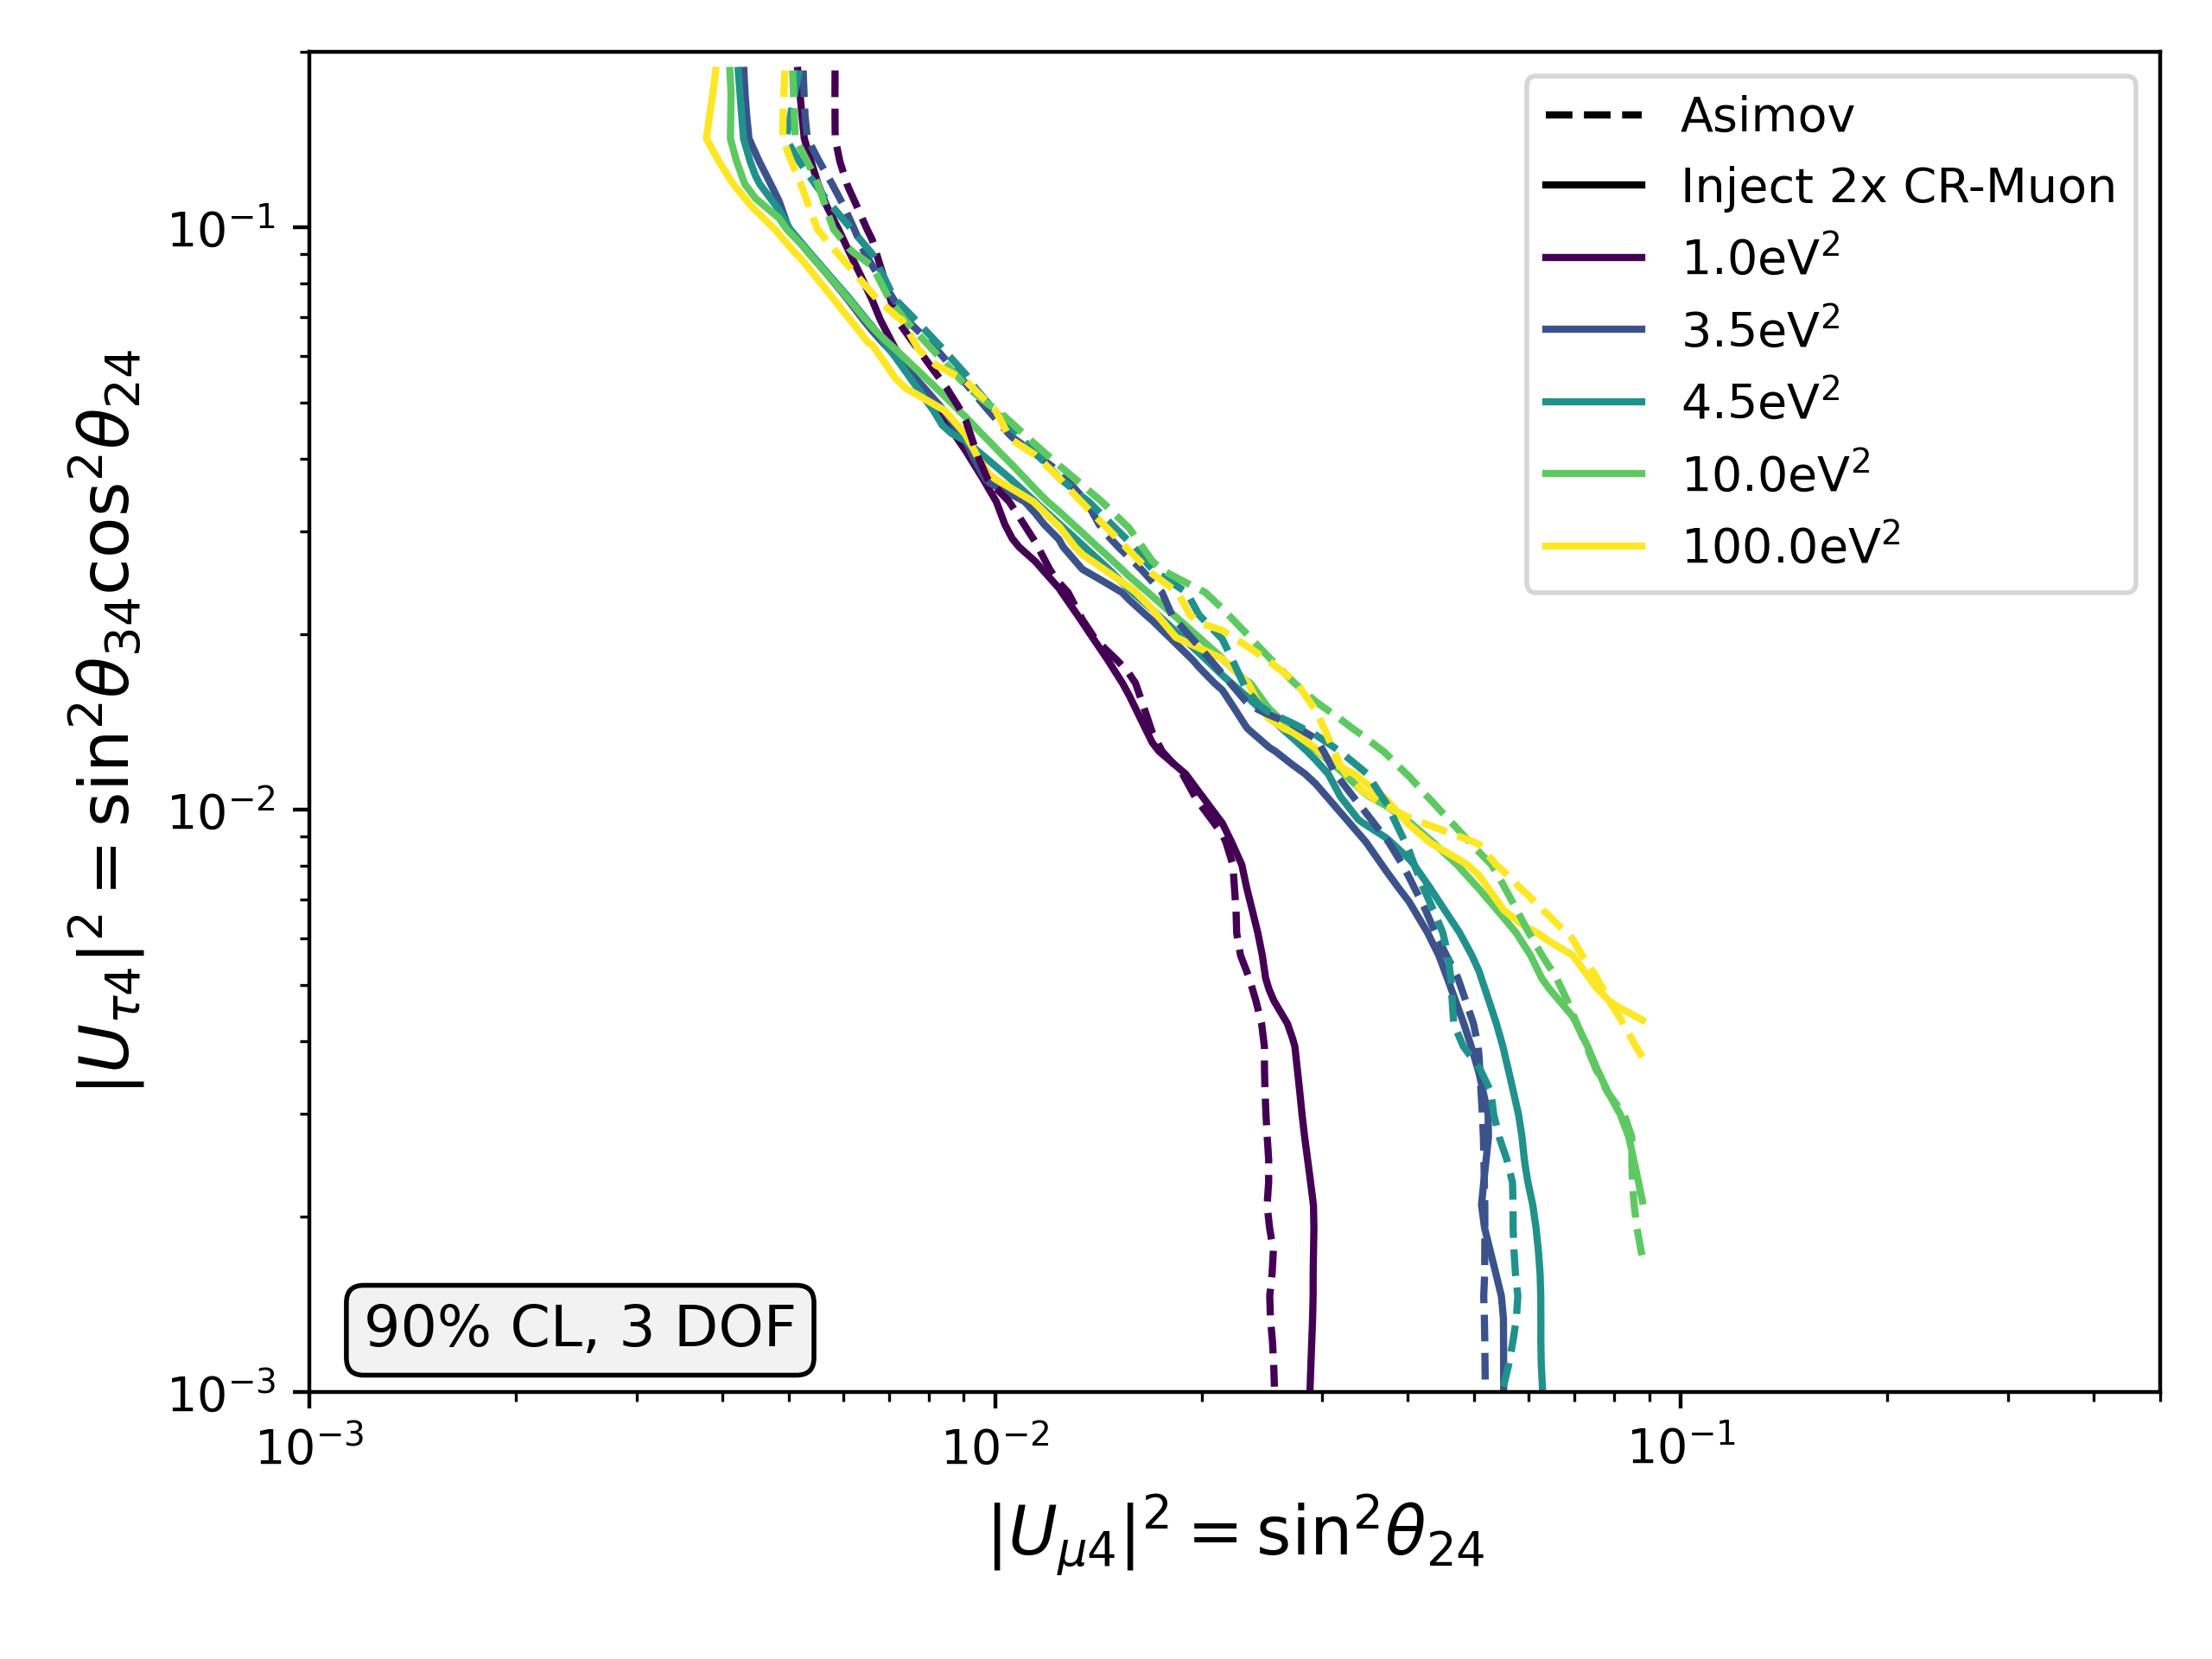
\includegraphics[width=0.45\linewidth]{figures/double_muon_mismodel_Realization_doublcr_sterile_0_cl0.9_dof3.png}
    \caption{The exclusion contours for situation (a) on the left and (b) on the right with the Asimov sensitivities provided for context}\label{fig:first_muon_sad}
\end{figure}  


\begin{figure}
    \centering
    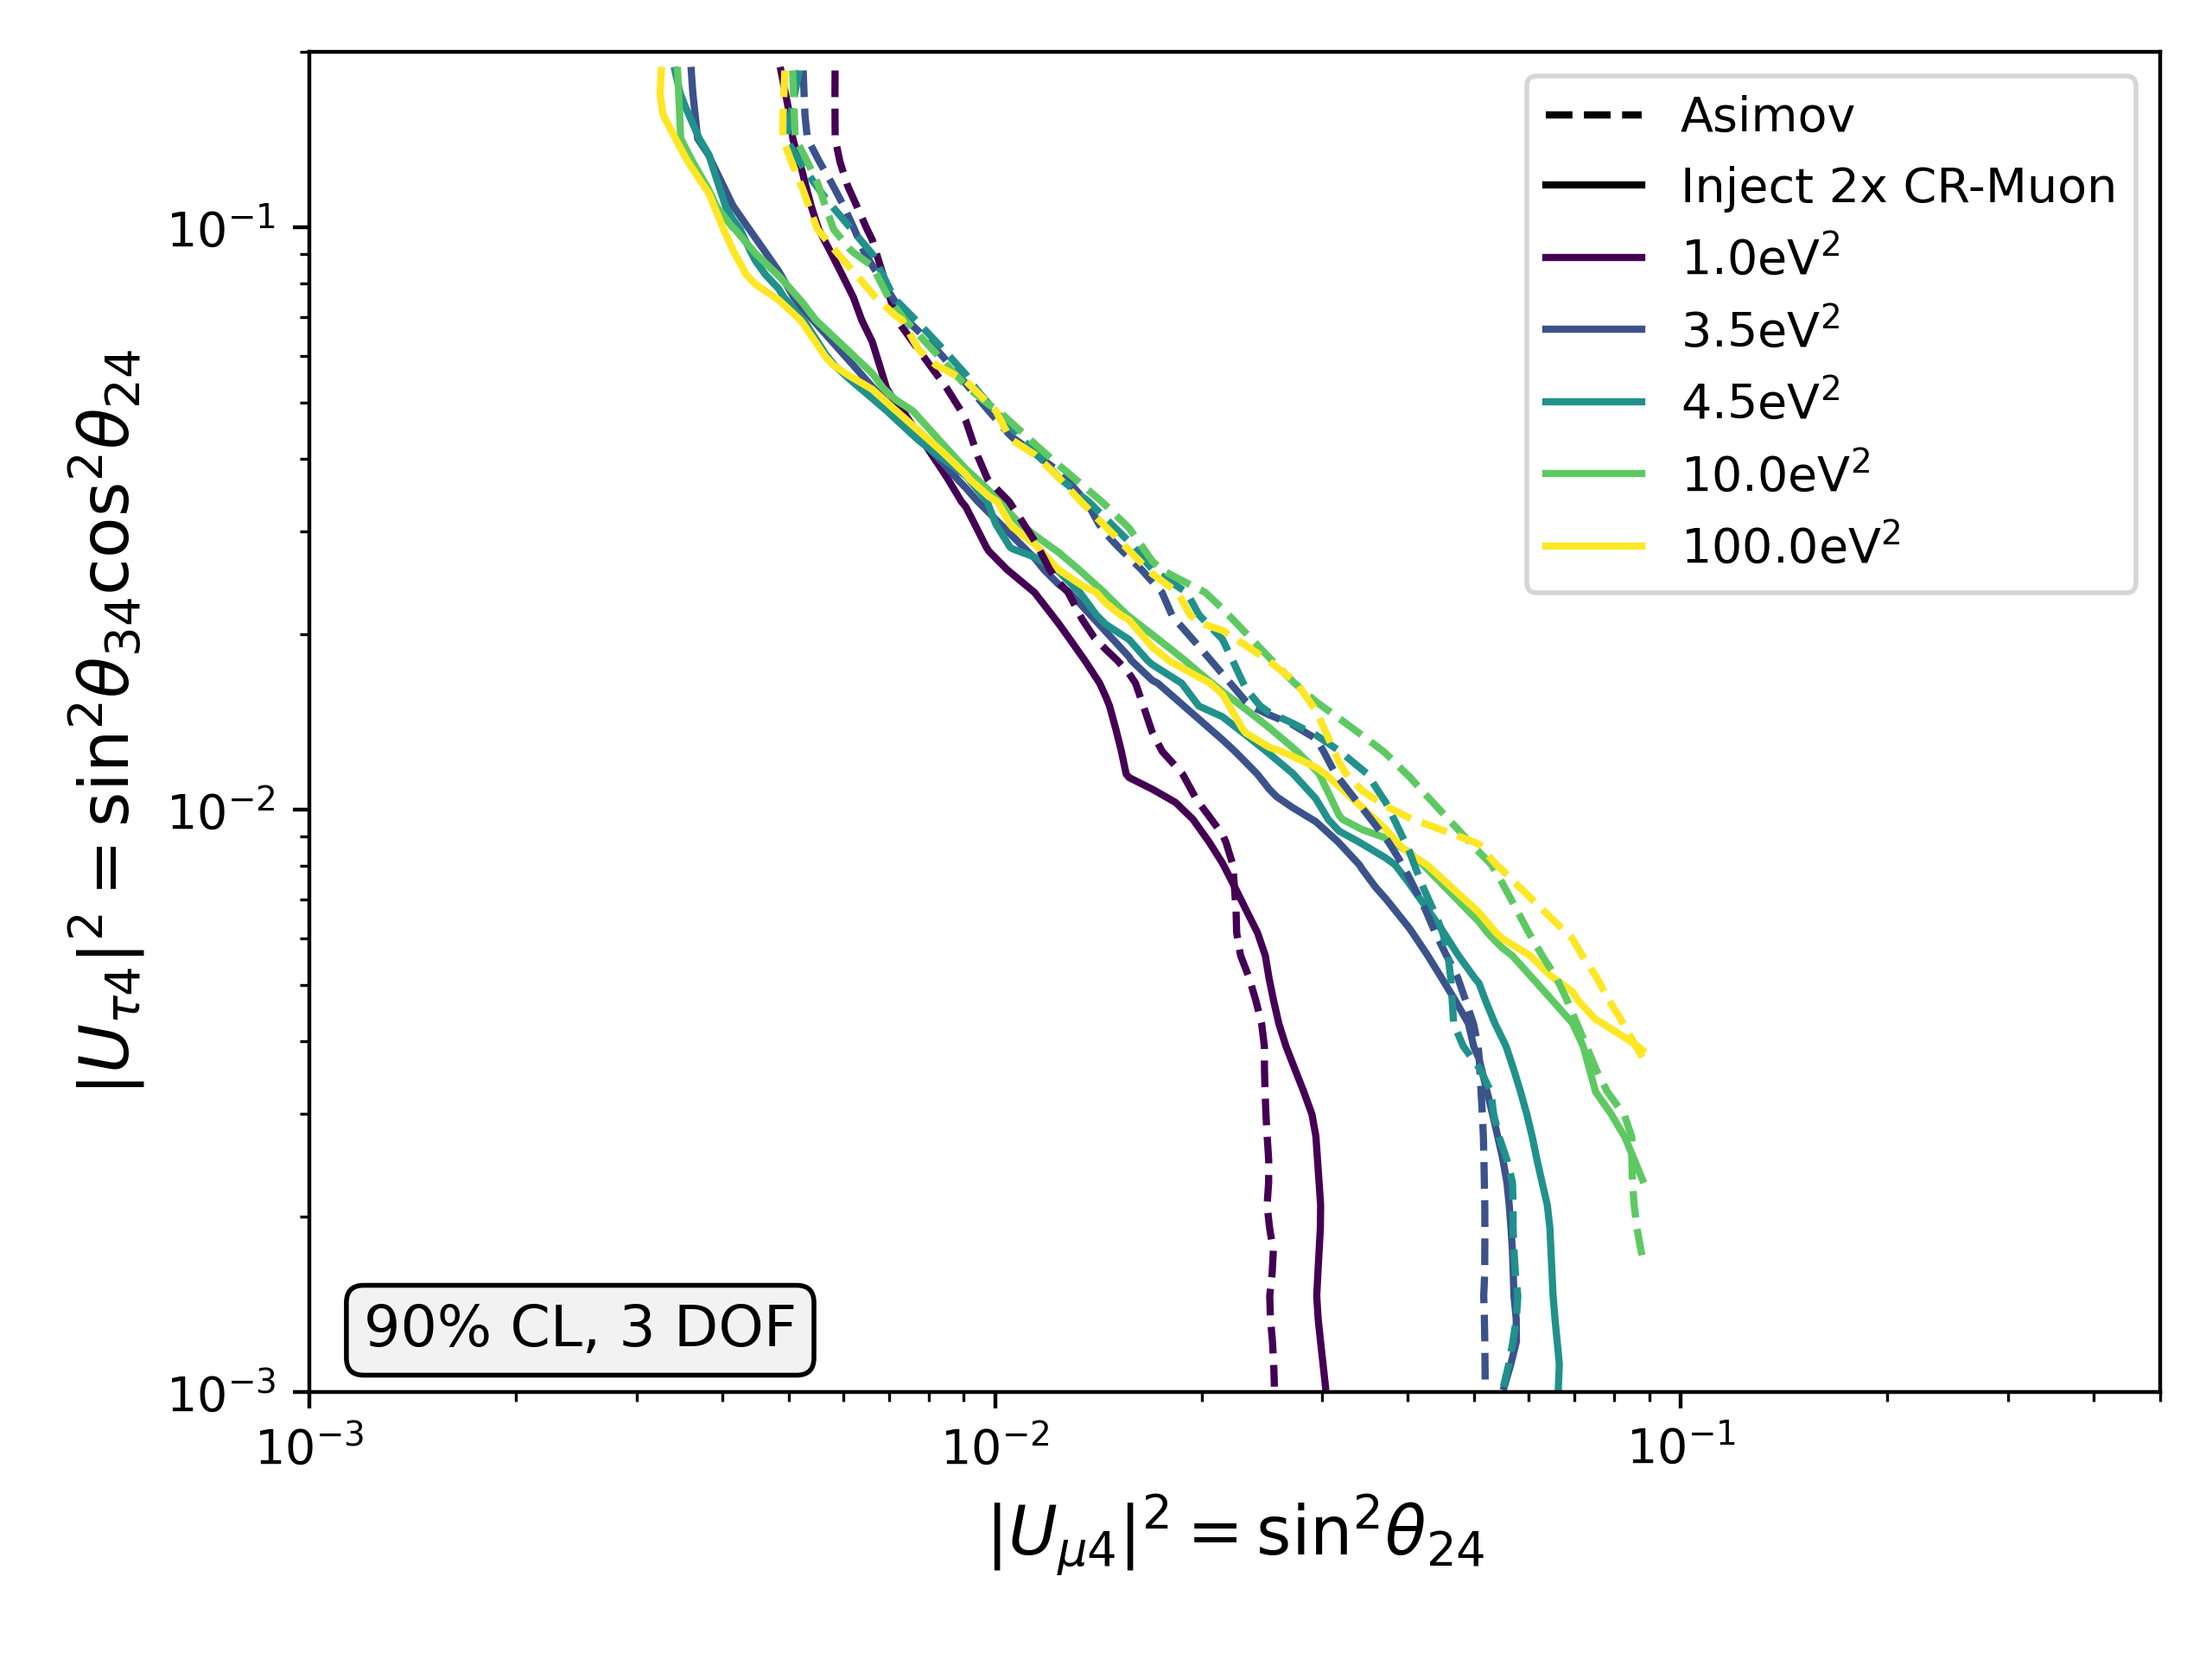
\includegraphics[width=0.7\linewidth]{figures/double_muon_mismodel_worse_Realization_doublcr_sterile_0_cl0.9_dof3.png}
    \caption{The exclusion contours for situation (c) with the Asimov sensitivities provided for context}\label{fig:last_muon_sad}
\end{figure}    


\section{Unblinding Procedure}

\begin{figure}
    \centering
    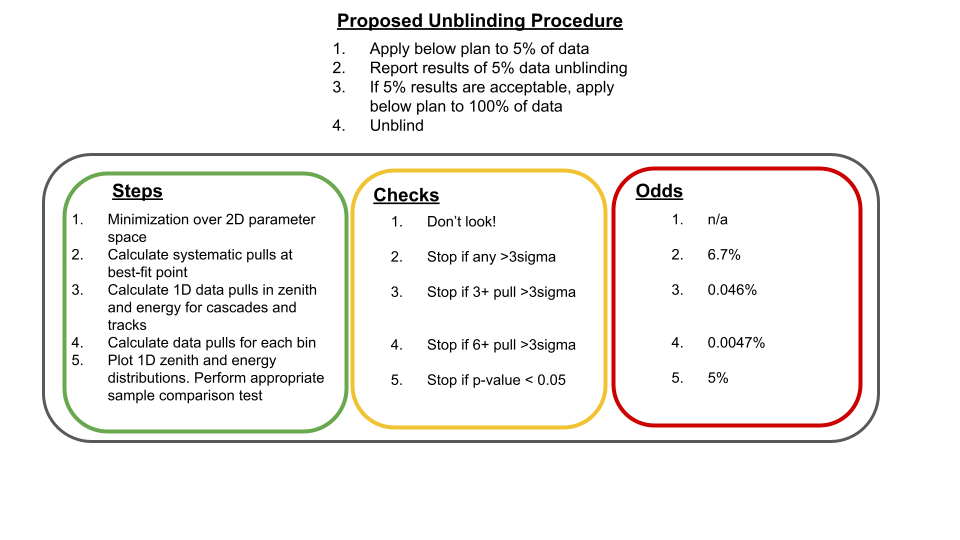
\includegraphics[width=0.7\linewidth]{figures/unblinding.png}
    \caption{The unblinding procedure used in this analysis and expected probabilities of satisfying the stop condition.}\label{fig:unblind}
\end{figure}

The unblinding procedure used in this analysis is shown in Figure~\ref{fig:unblind}. 
First, a full 3D fit-scan is applied while fitting to only 5\% of the full dataset. 
No best fit parameters or likelihoods are reported. 
At the best fit point, if any nuisance parameters have a fit value more than $3\sigma$ away from their central values, we stop. 
Then we count the number of bins whose best fit values are more than $3\sigma$ away from their expected value; if more than 3 satisfy this condition, we stop. 

\subsection{5\% Data Blind Fit Results}

First, a fit on 5\% of the data was carried out to validate basic functionality and ensure no glaring inconsistencies between data and MC exist. 
A full fit scan is carried out over the full new-physics phase space, and the best-fit point is found. 
The nuisance parameter pulls are determined, and shown in Figure~\ref{fig:pulls_5p}; none pulled above $3\sigma$.

Then the 1D pulls were calculated and the 1D distributions calculated; none pulled above $3\sigma$. 
These are shown in Figure~\ref{fig:1d_5p_distrib}.
Finally, the 2D distribution of pulls were calculated and are shown in Figure~\ref{fig:2d_5p_distrib}.
Again, nothing pulled above $3\sigma$. 
P-values were calculated and all found to be within the required bounds. 
Since all checks passed, we proceeded to blind fits on 100\% of the data. 

\begin{figure}
    \centering
    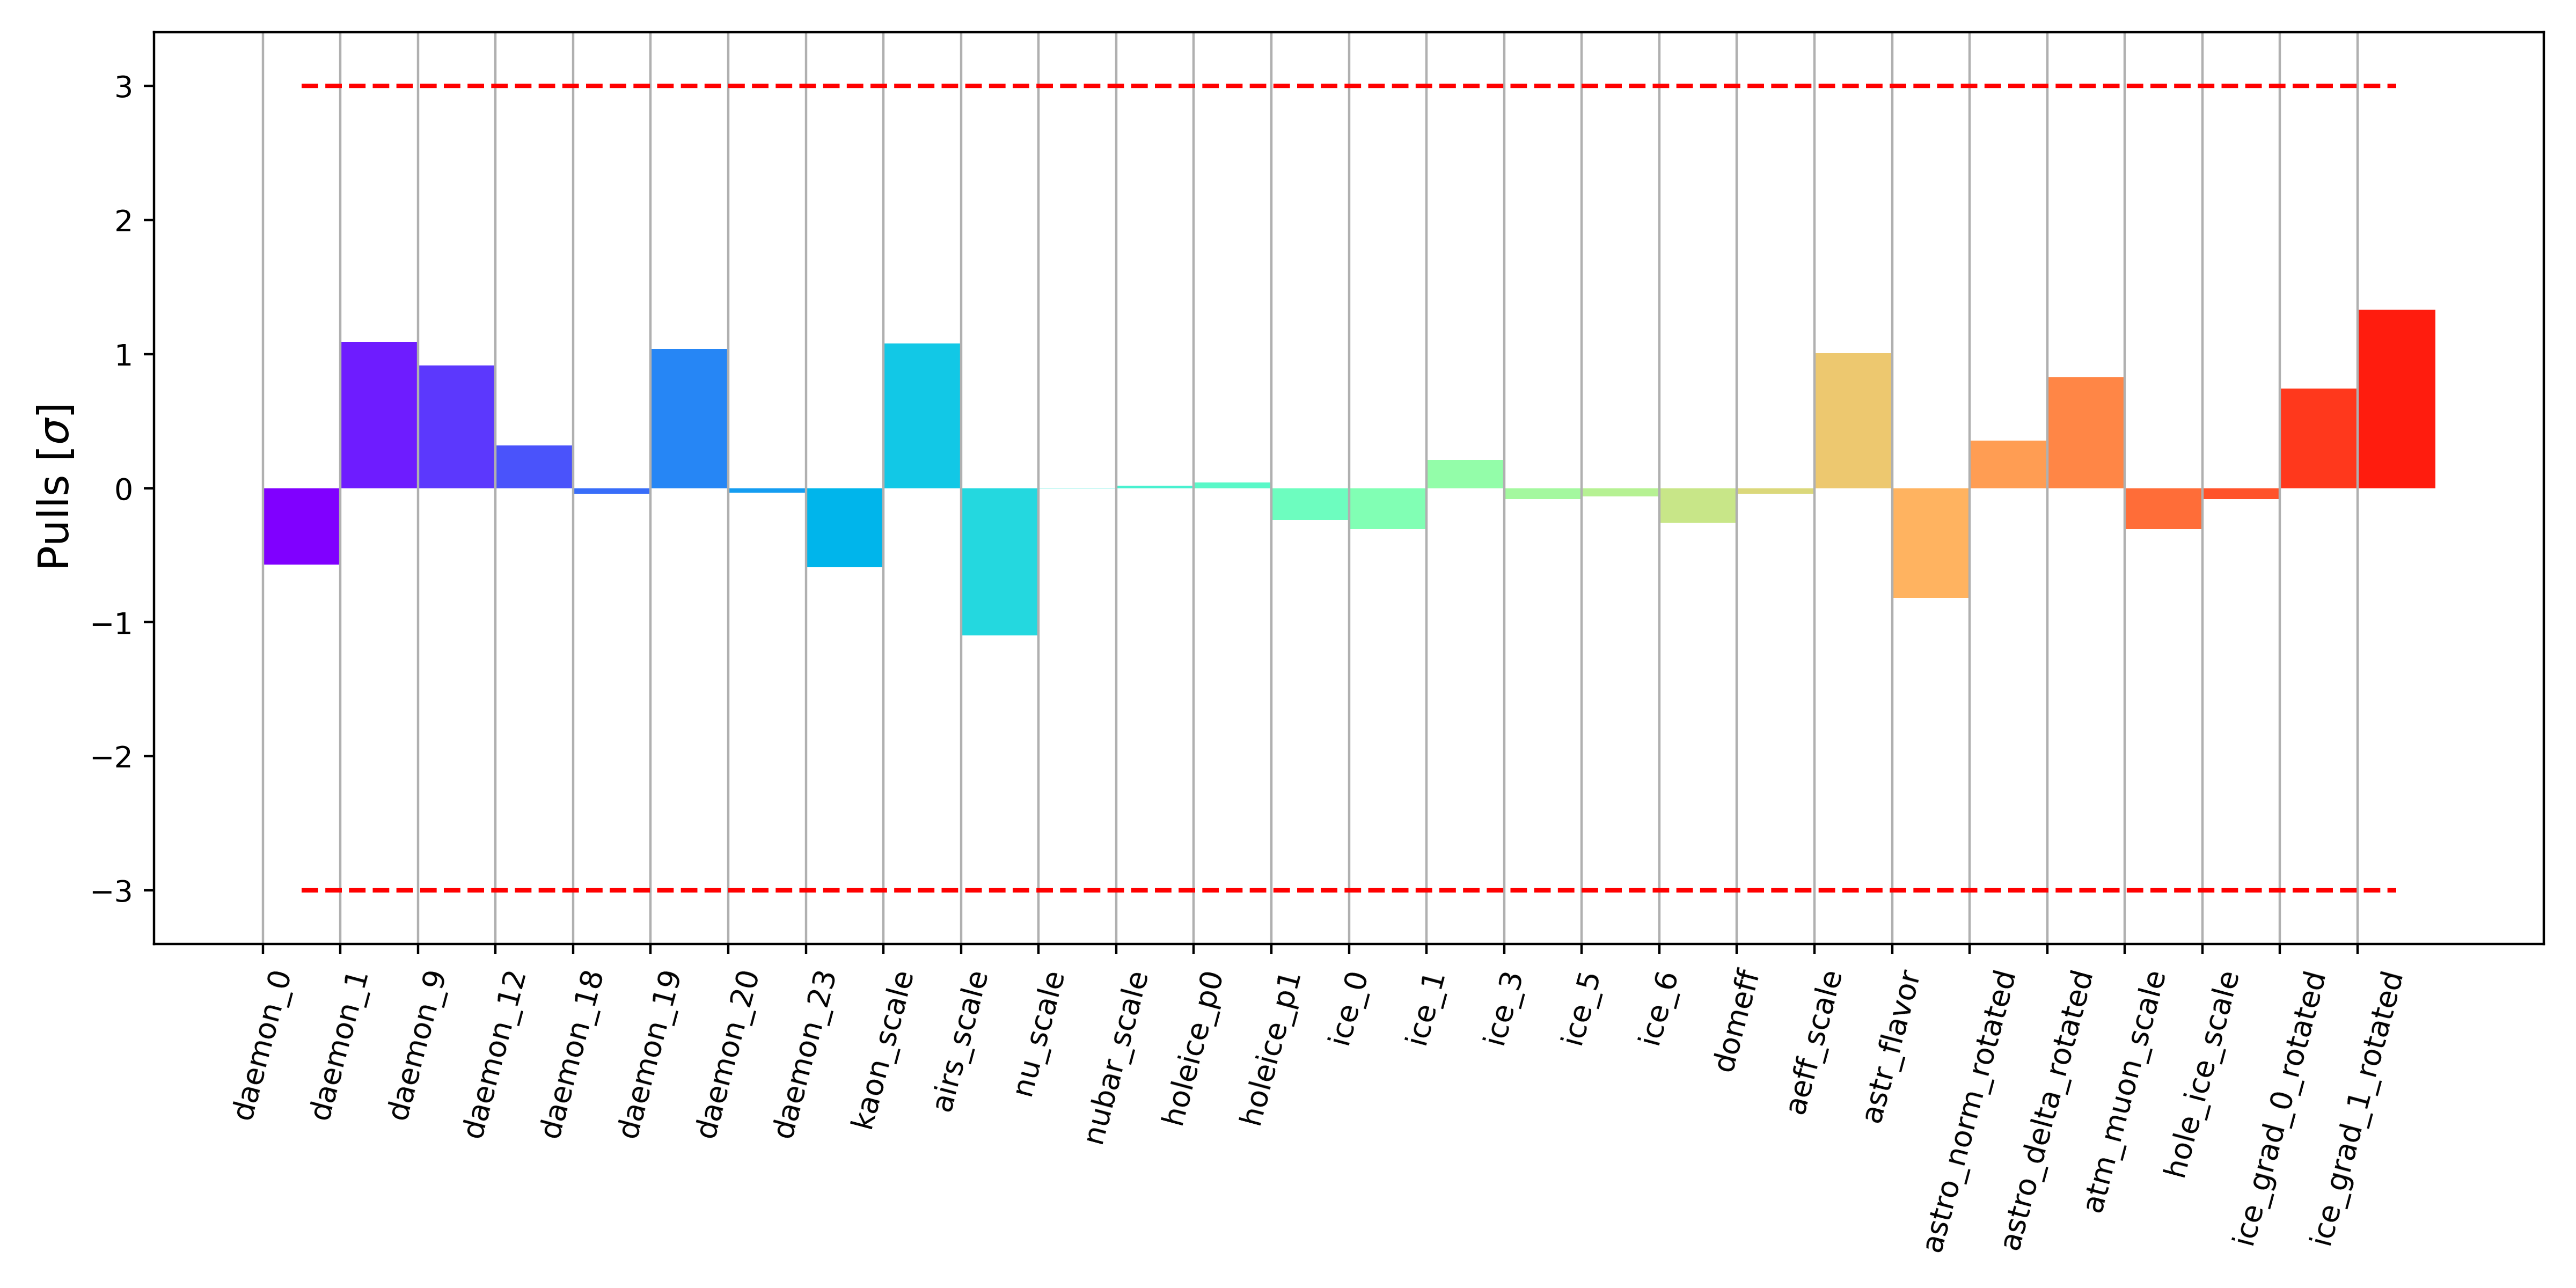
\includegraphics[width=0.9\linewidth]{./figures/blindfit/pulls_IC86_data_five_percent_joint_data_5p_with_flavor_update_fix.png}
    \caption{The nuisance parameter pulls at the best fit to 5\% of the data.}\label{fig:pulls_5p}
\end{figure}

\begin{figure}
    \centering
    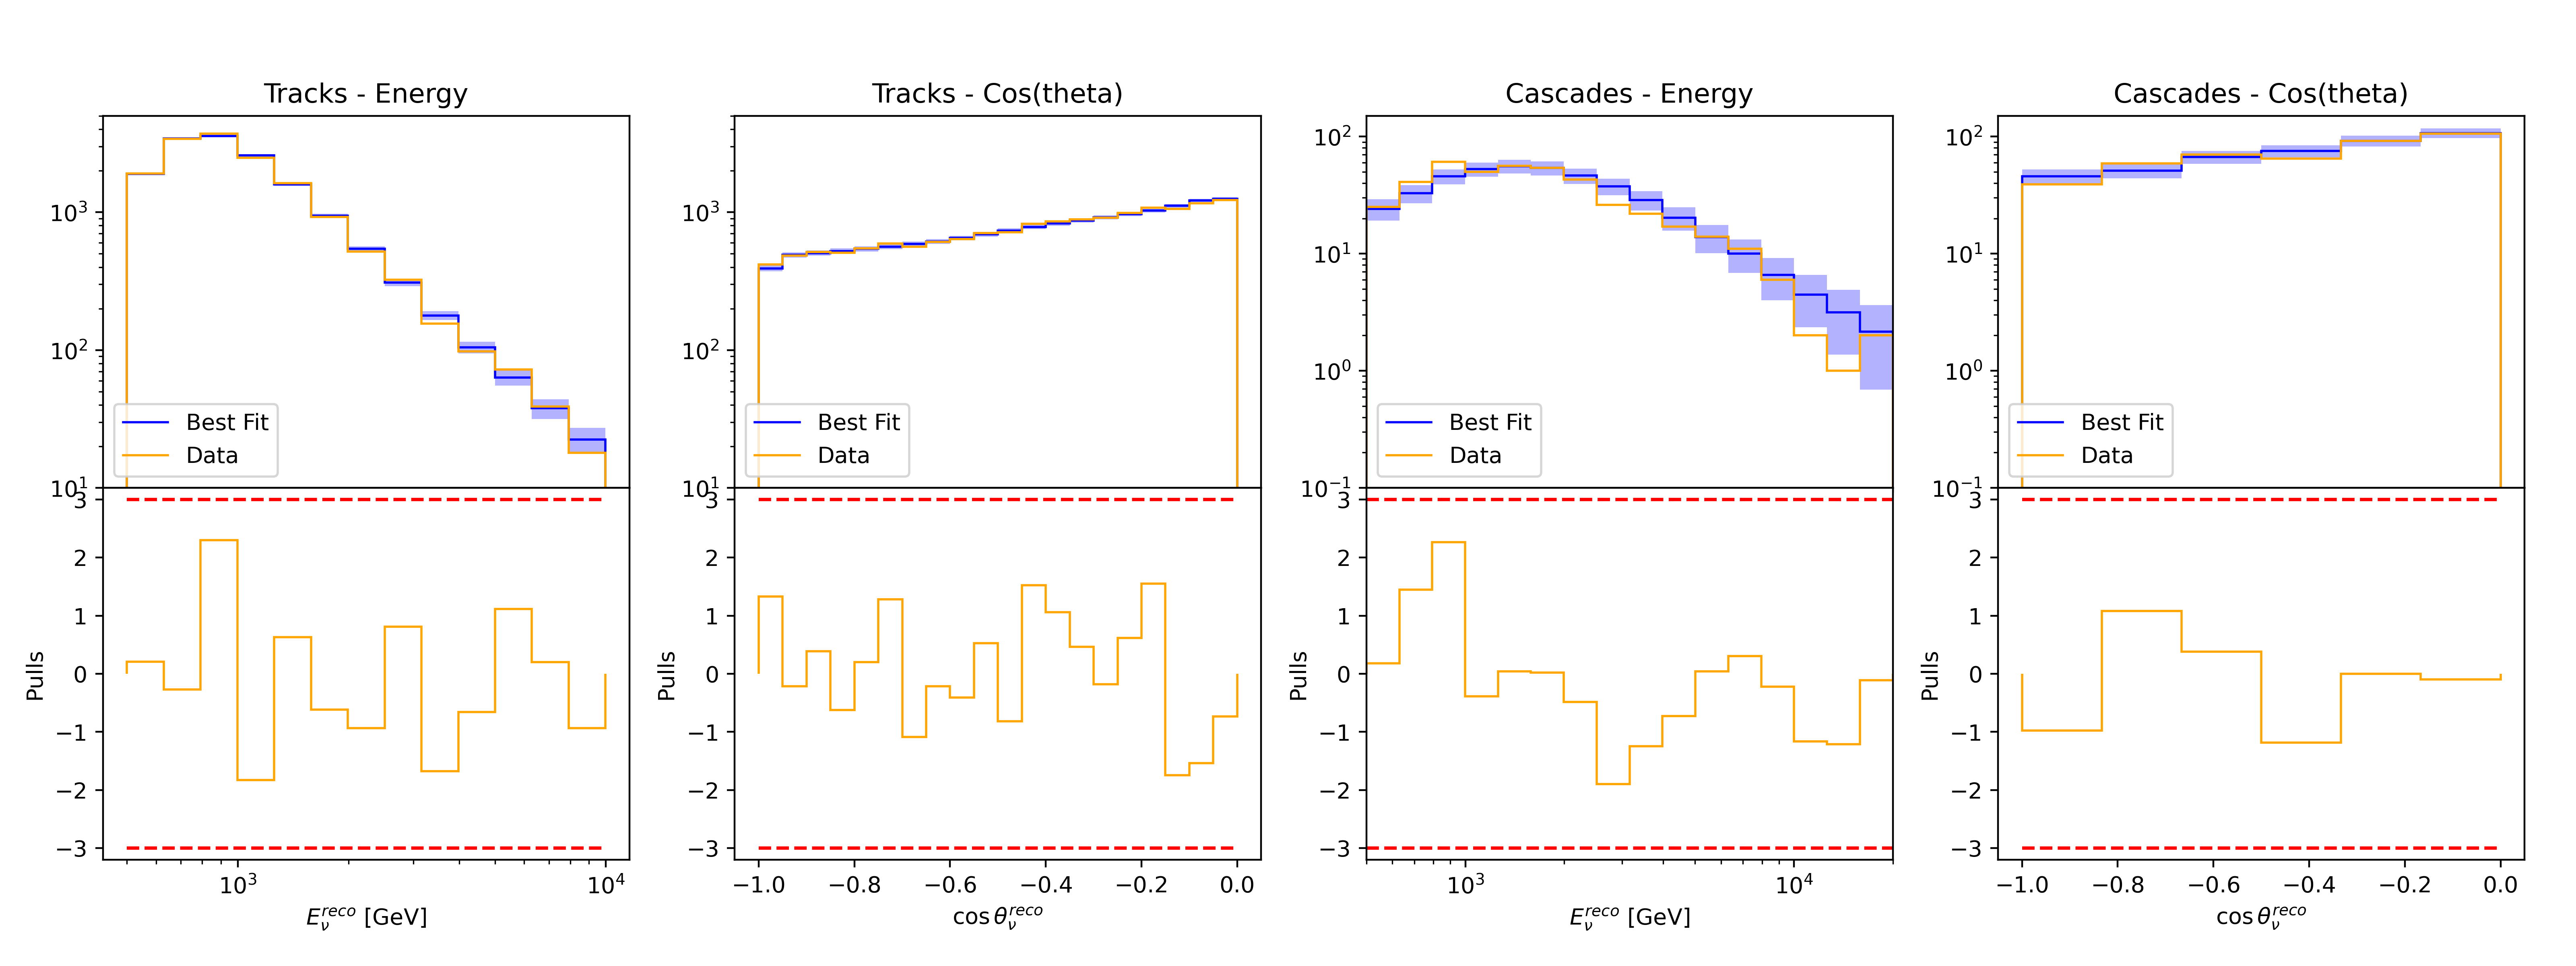
\includegraphics[width=0.9\linewidth]{./figures/blindfit/goodness_joint_data_5p_with_flavor_update_IC86_data_five_percent.png}
    \caption{The 1D pulls and distribution of 5\% of the data.}\label{fig:1d_5p_distrib}
\end{figure}

\begin{figure}
    \centering
    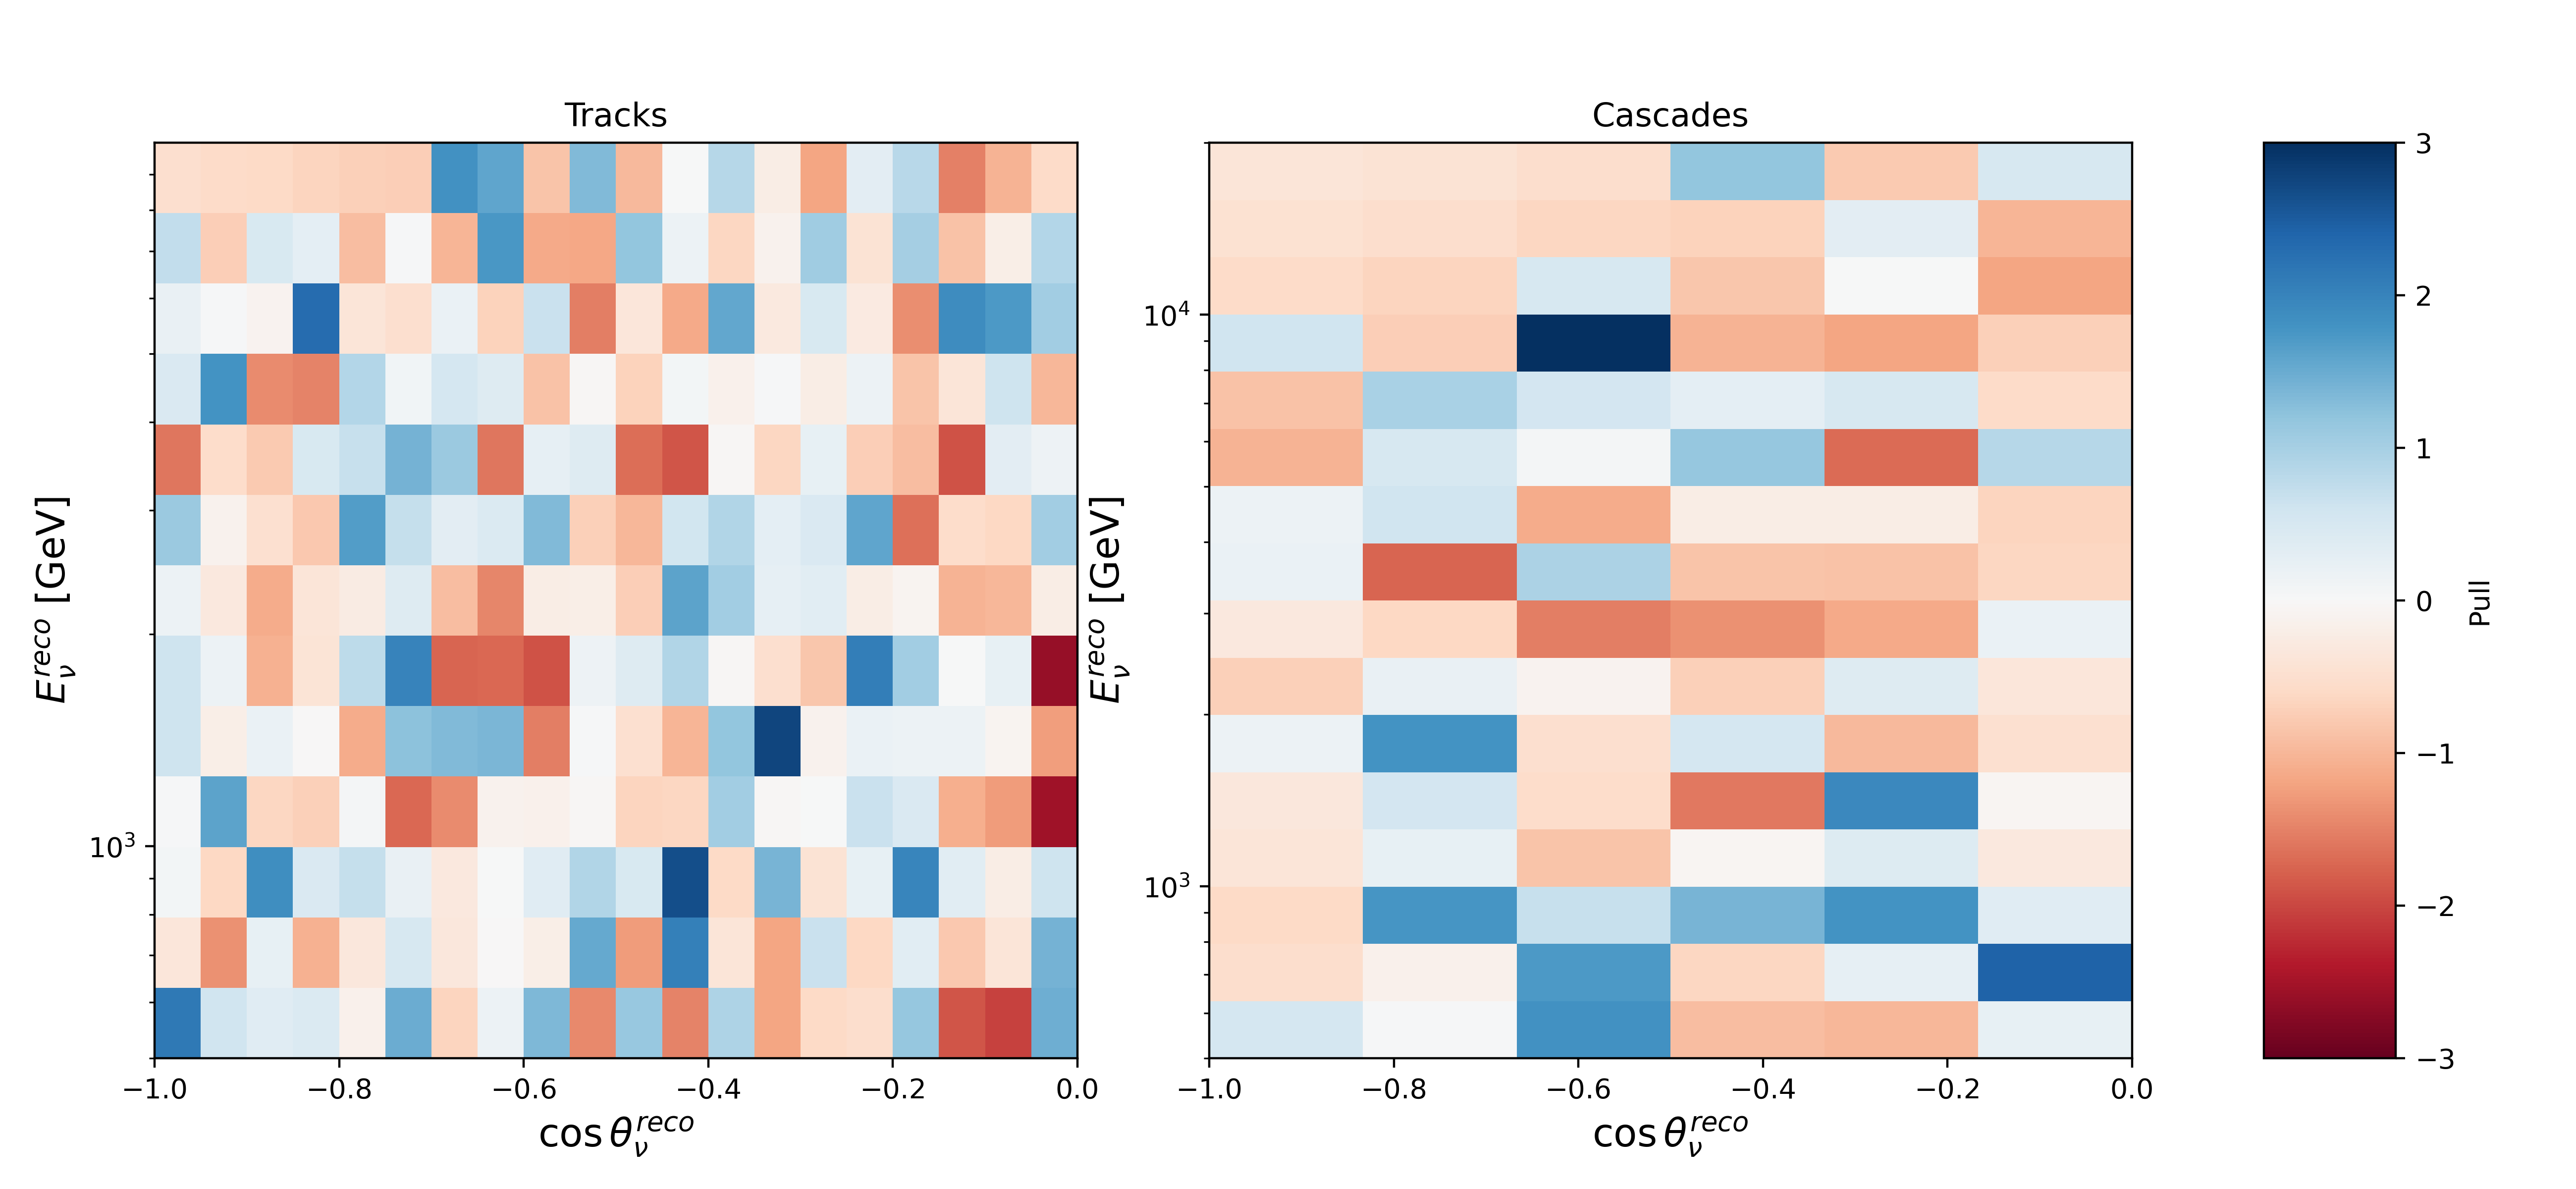
\includegraphics[width=0.9\linewidth]{./figures/blindfit/2dpulls_joint_data_5p_with_flavor_update_fix_IC86_data_five_percent.png}
    \caption{The 2D pulls and distribution of 5\% of the data.}\label{fig:2d_5p_distrib}
\end{figure}

\subsection{100\% Data Blind Fit Results}\label{sec:ice_chaos_ohgod}

Before looking at the exclusion contours and ``unblinding,'' we first validate that the fit is sensible. 
Similar to before, the nuisance parameter pulls were calculated and then the pulls in the 1D distributions. 
These are shown in Figure~\ref{fig:pulls_100p} and~\ref{fig:1d_100p_distrib}.
For the cascades, one bin pulled at $3\sigma$, and as a consequence the p-value dropped to 0.007: a stop condition. 

\begin{figure}
    \centering
    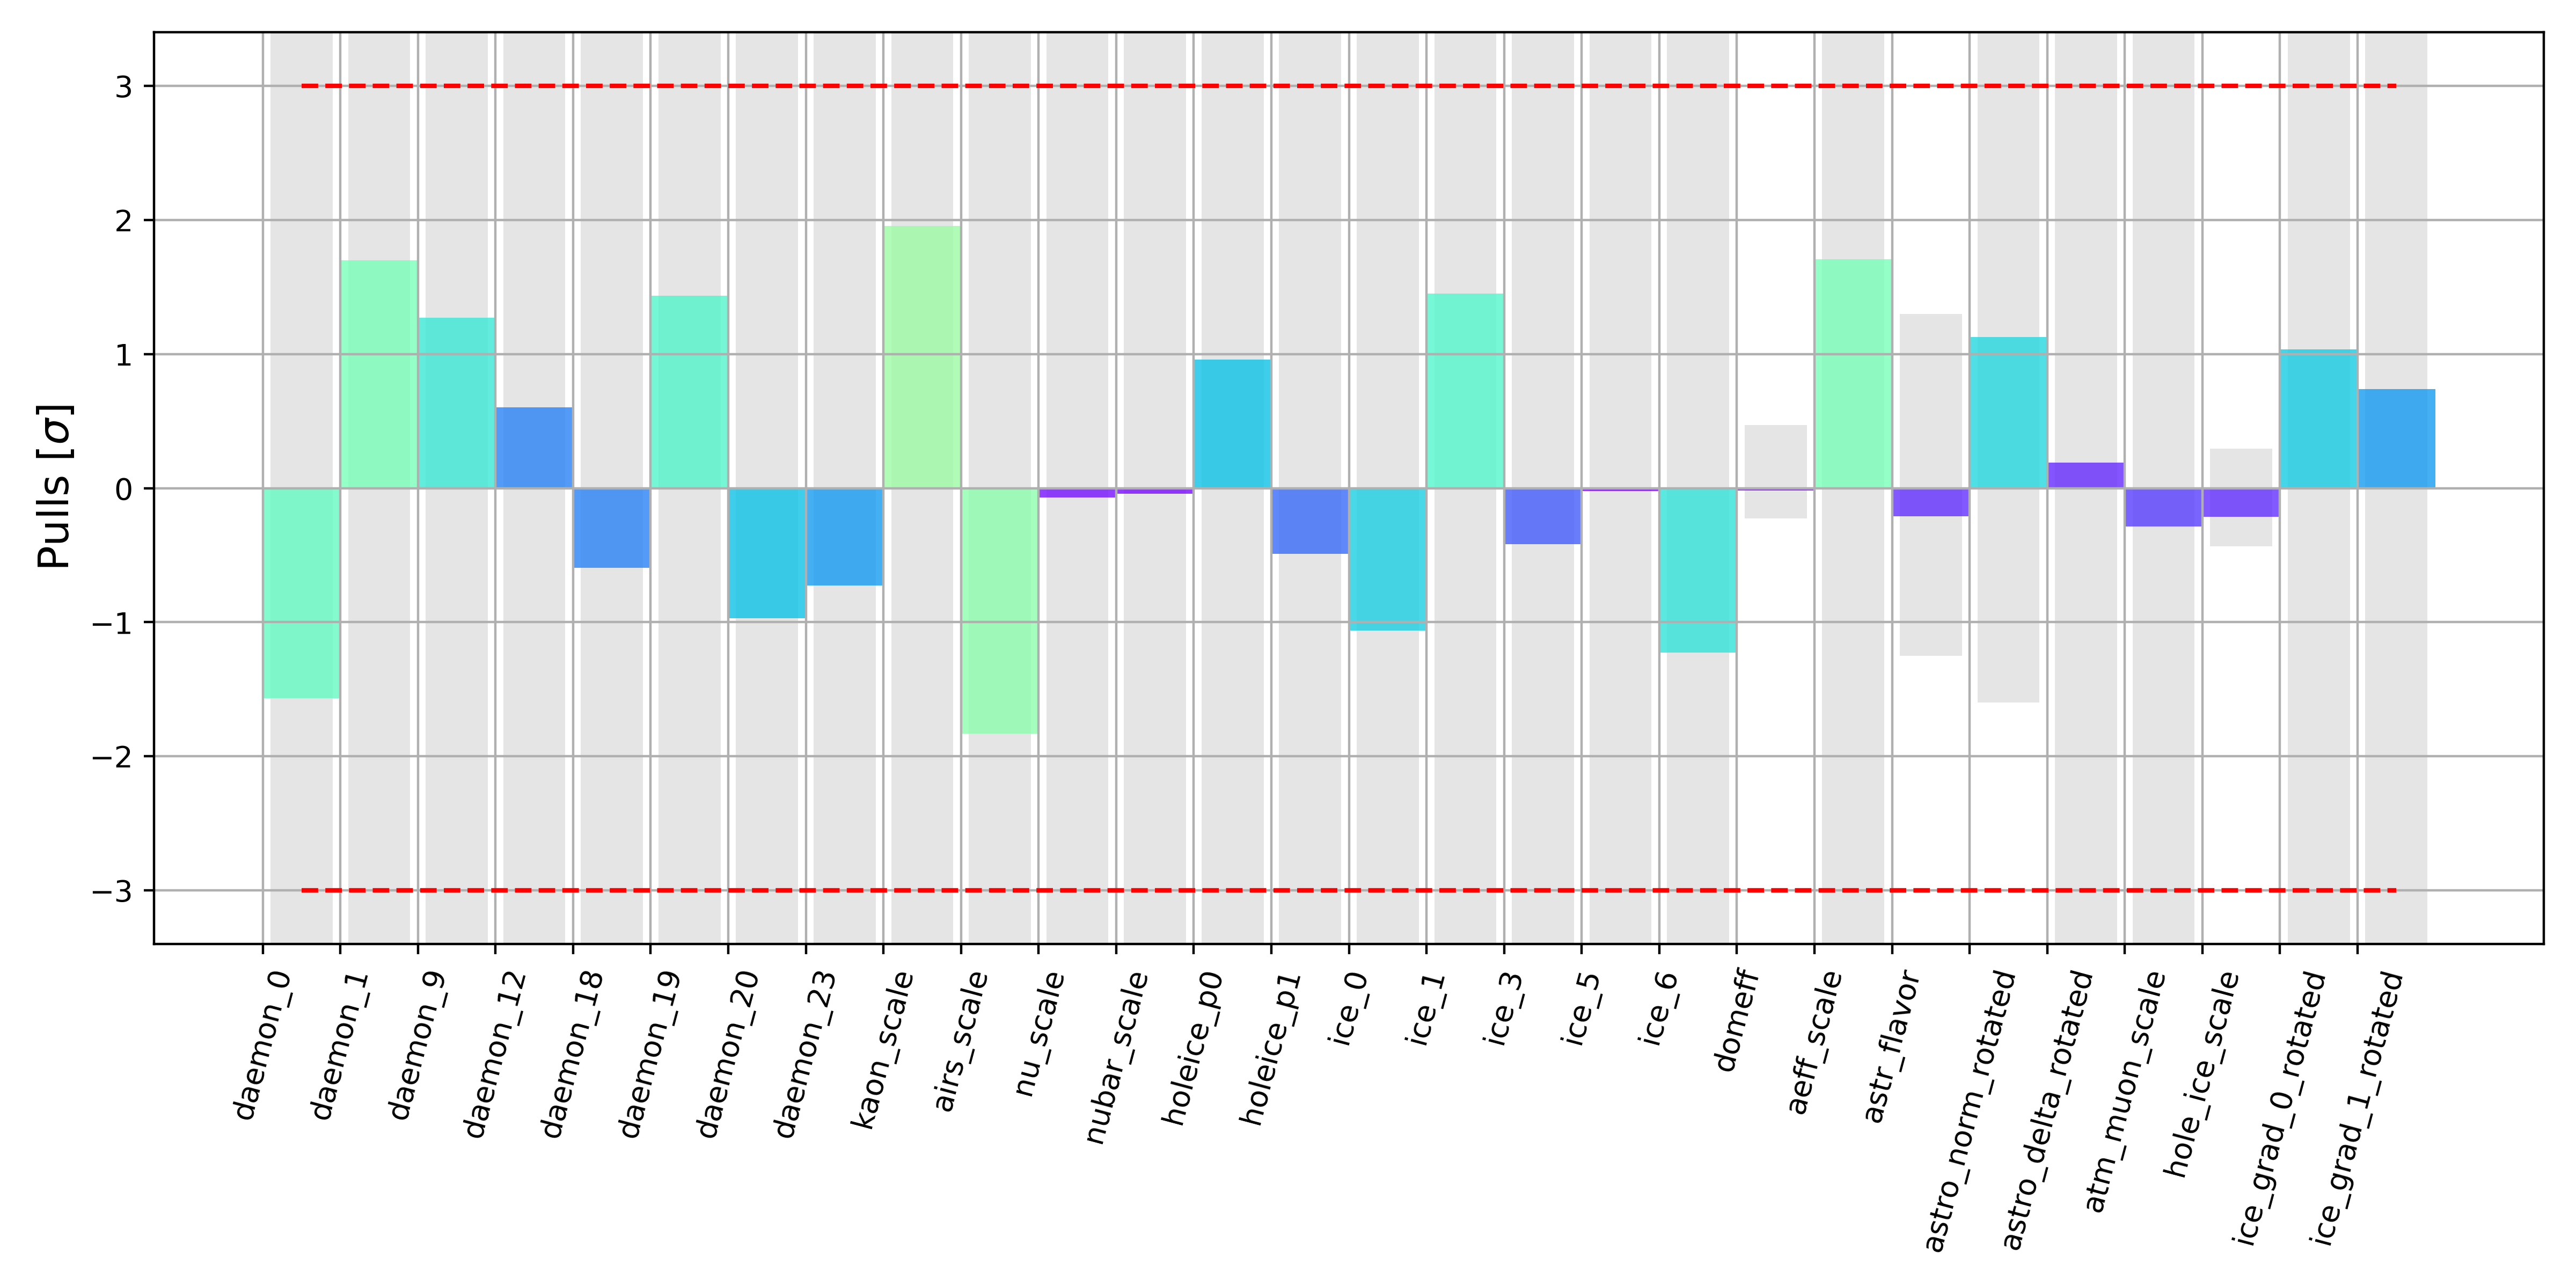
\includegraphics[width=0.9\linewidth]{./figures/pulls_IC86_data_full_joint_data_full.png}
    \caption{The nuisance parameter pulls at the best fit to 5\% of the data.}\label{fig:pulls_100p}
\end{figure}


\begin{figure}
    \centering
    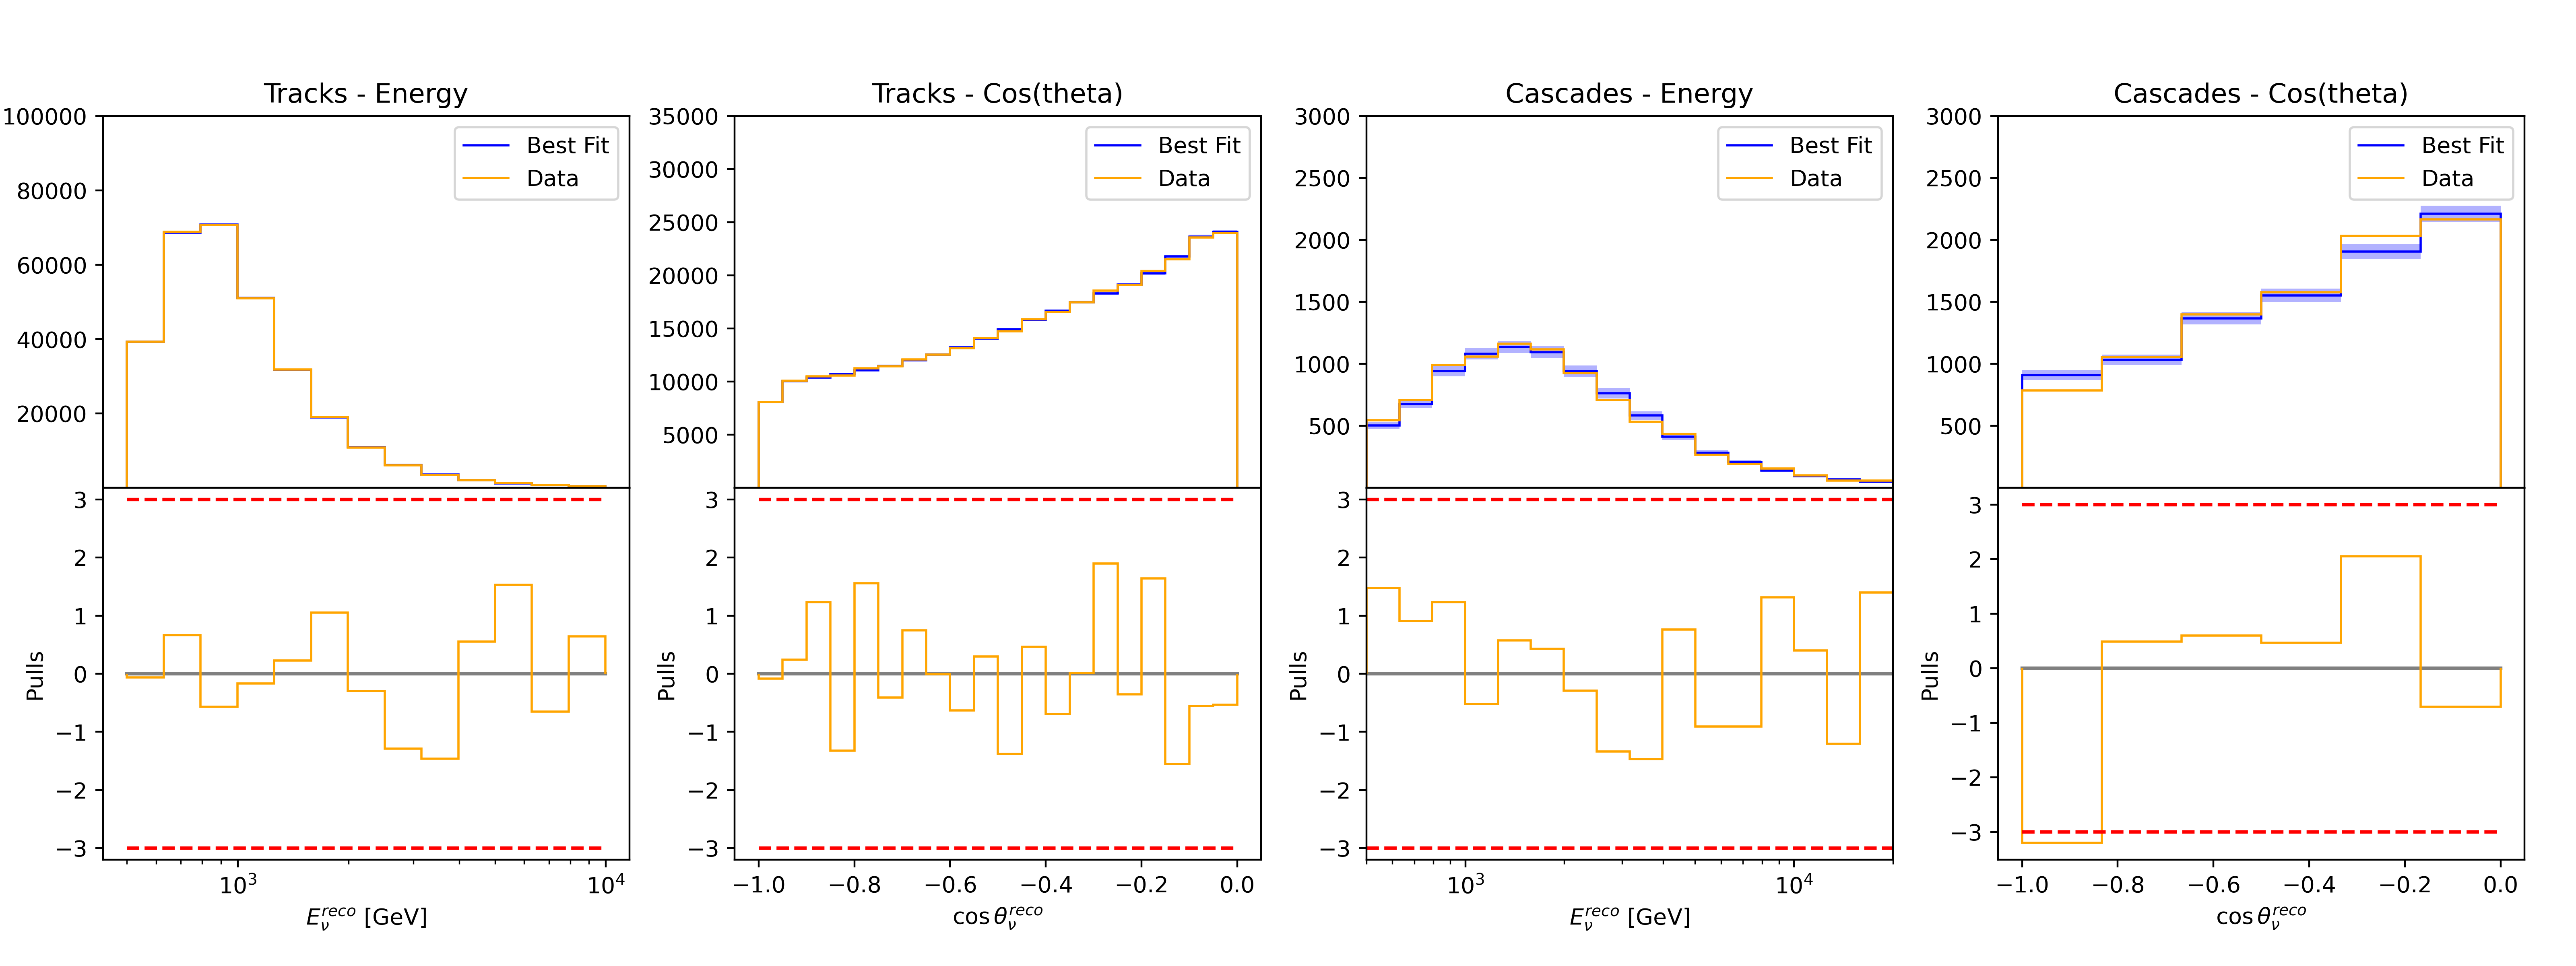
\includegraphics[width=0.9\linewidth]{./figures/goodness_joint_data_full_IC86_data_full.png}
    \caption{The 1D pulls and distribution of 100\% of the data.}\label{fig:1d_100p_distrib}
\end{figure}


To investigate this, we suspected an ice-modeling may be a factor.
Two ice models were introduced previously in Section~\ref{sec:the_ice_stuff}.
The track and cascades samples both had relied on the legacy Spice 3.2.1; more recently, however, the improved BFR v2 model had been shown to predict differing photon-DOM counts as a function of $\cos\theta$.  
This is shown in Figure~\ref{fig:zenith_bfr}.

\begin{figure}
    \centering
    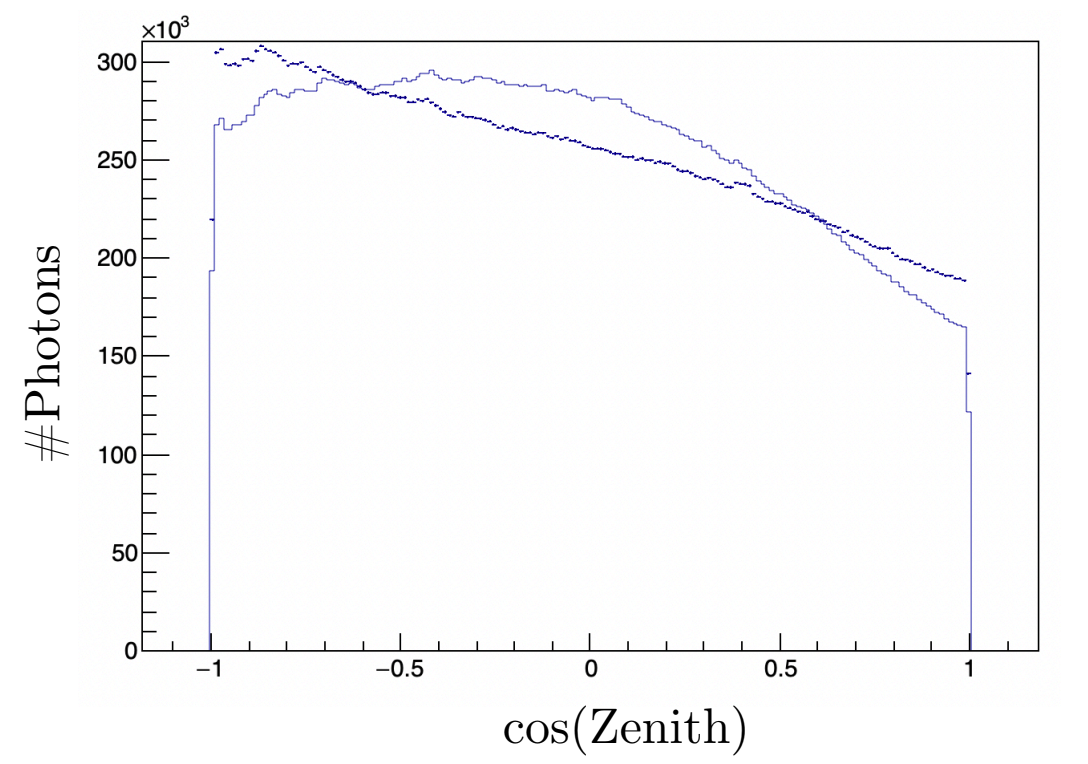
\includegraphics[width=0.75\linewidth]{./figures/ice_investigate/zenith_bfr.png}
    \caption{Differences in photon counts for Spice 3.2.1 (dark blue line) and BFR v2 (light blue line).}\label{fig:zenith_bfr}
\end{figure}

Motivated by these differences, a small sample of 5000 cascades were generated for $\cos\theta\in\left[-1.0, -0.9\right]$ and $E_{\nu}^{true}\in\left[1\text{TeV}, 2\text{TeV}\right]$. 
Using the exact same MC events and energy losses, photon propagation was performed separately using the Spice 3.2.1 and BFR v2 models to generate two versions of the sample.
The detector simulation, trigger simulation, filter simulation, and even reconstruction was then carried out for each of the two versions. 
Reconstructed event rates are shown in Figure~\ref{fig:icetest}; a disagreement is observed between the two sample predictions. 
This disagreement further supported a systematic difference in the predictions between the two ice models. 

\begin{figure}
    \centering
    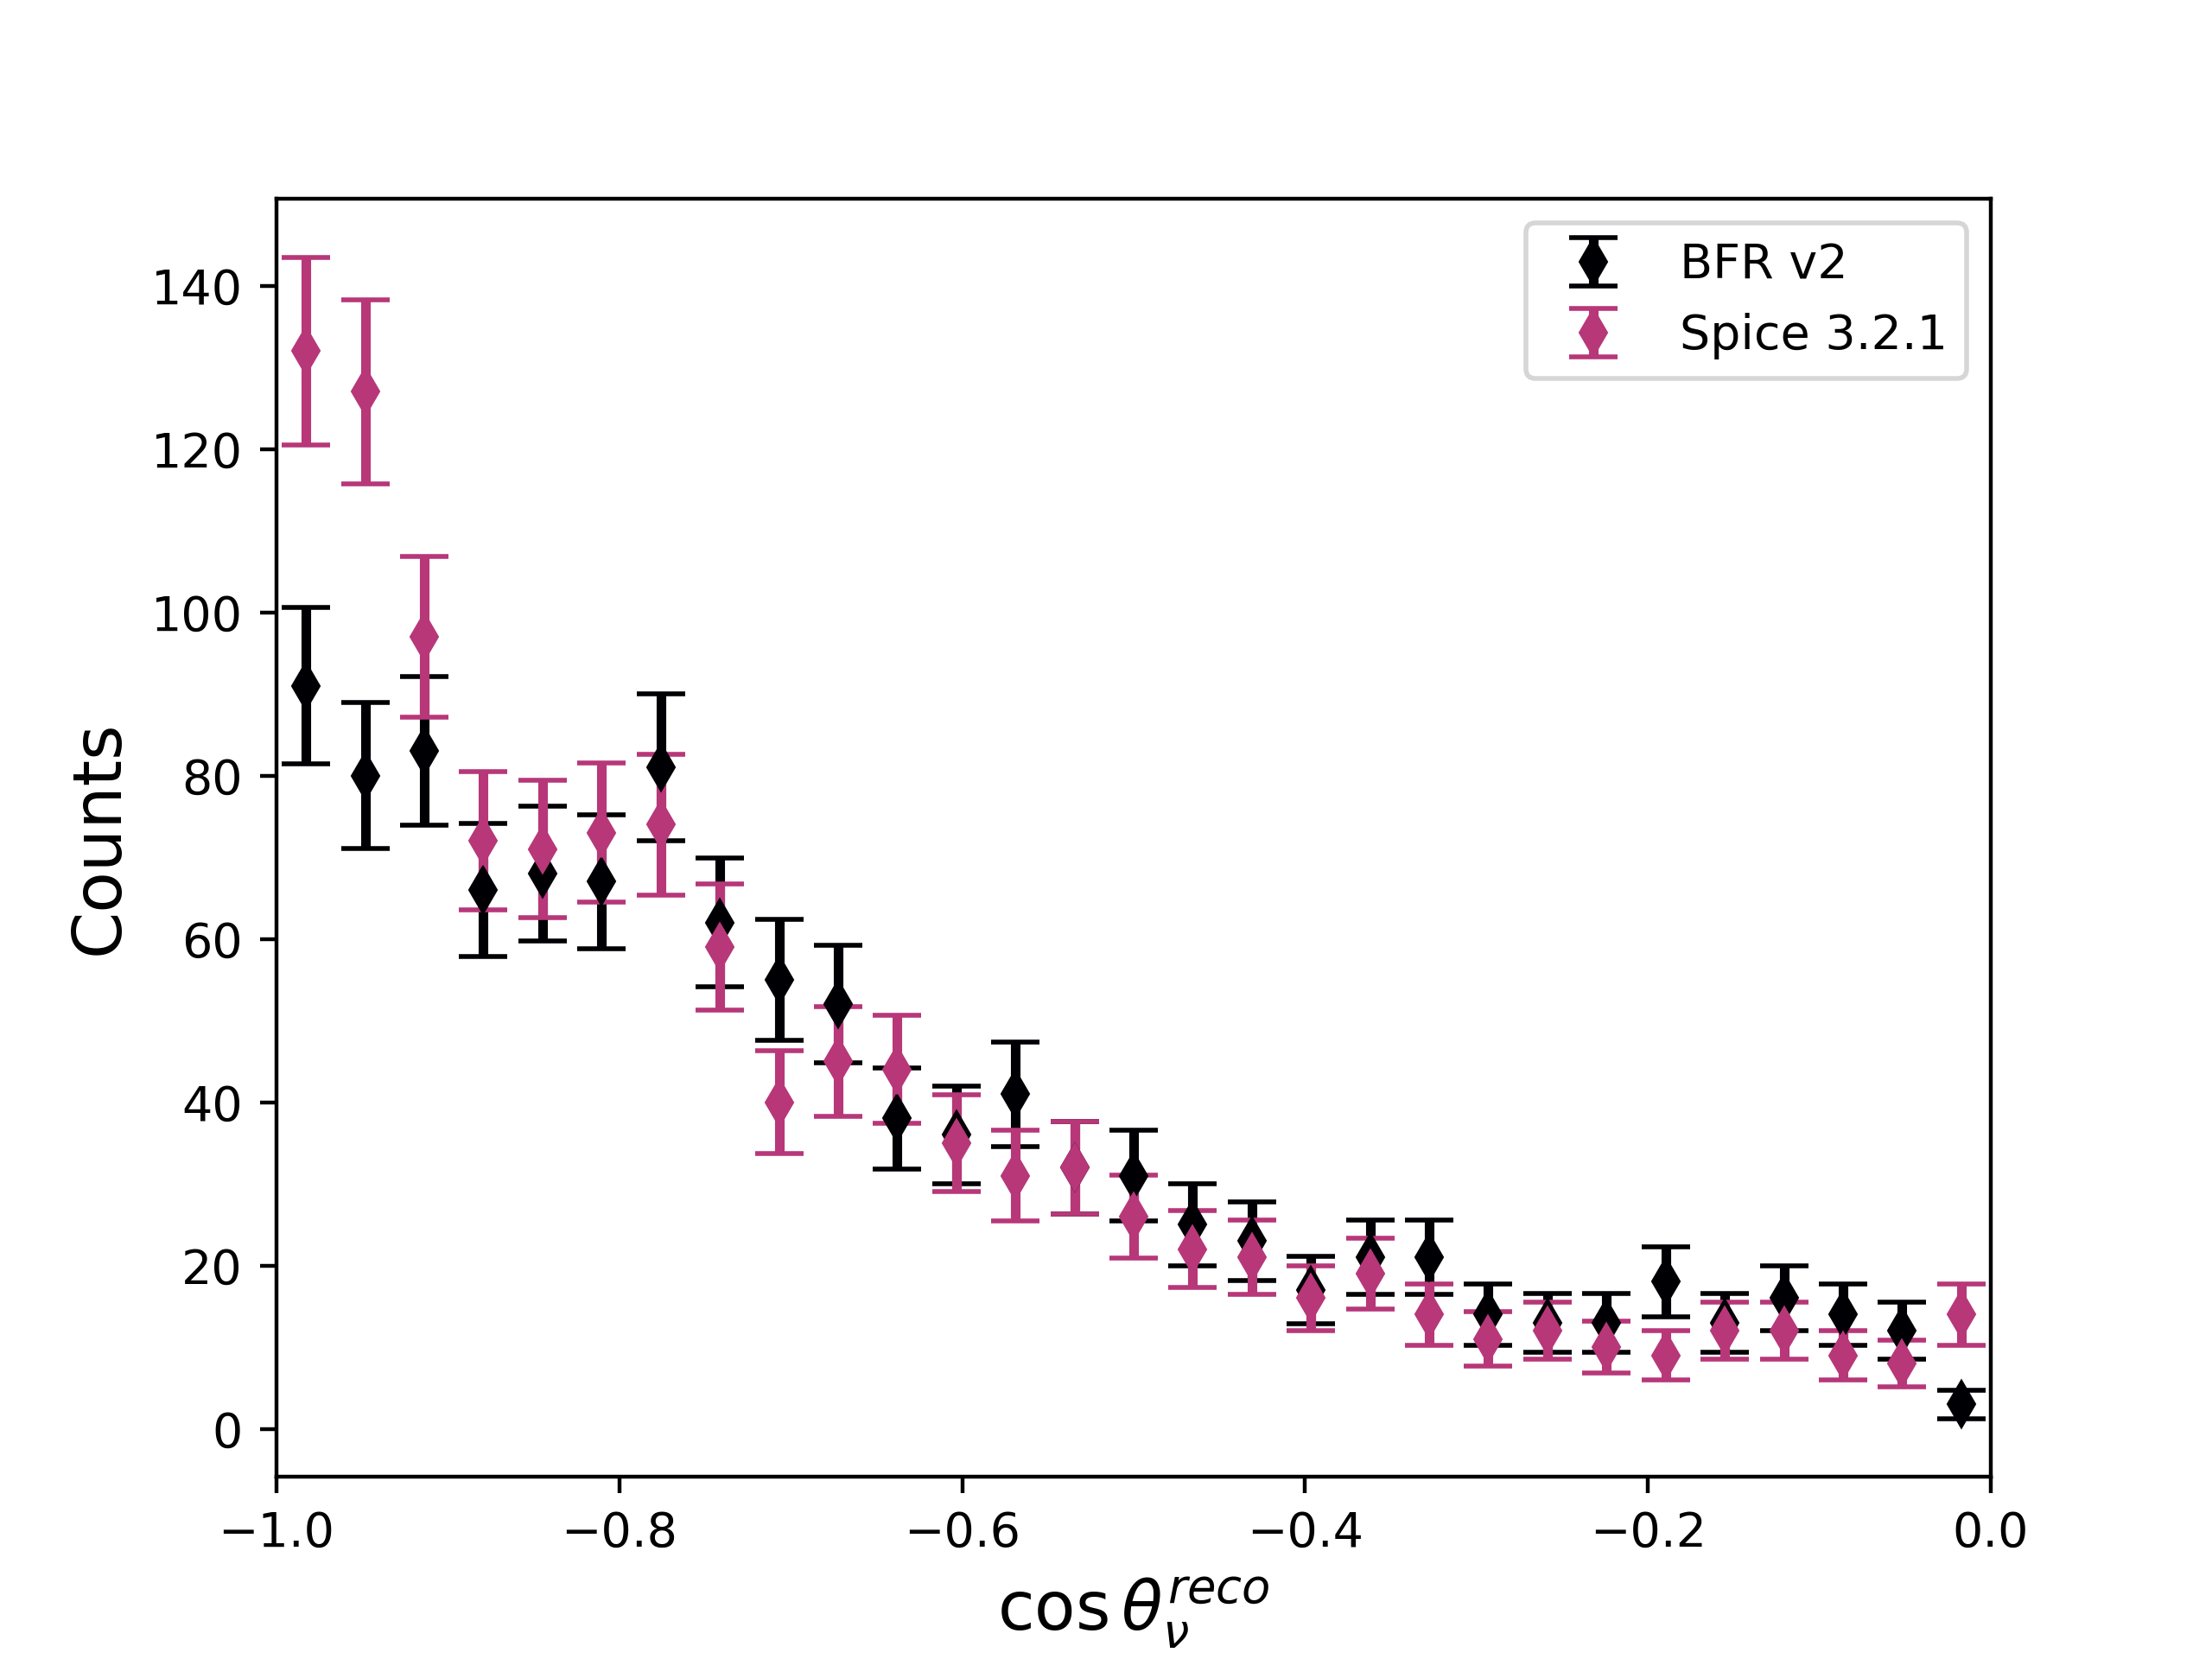
\includegraphics[width=0.8\linewidth]{figures/ice_investigate/icetest.png}
    \caption{Reconstructed event rates (unweighted) for the BFR v2 and Spice 3.2.1 MC sample versions; error bars are show MC statistical error.}\label{fig:icetest}
\end{figure}

A separate, low-statistics, MC sample had been prepared internally in IceCube as part of a separate mismodeling test. 
This sample had been prepared using the BFR v2 ice model, and so we ran this analysis' cascade reconstruction and final level filters on the MC files. 
BFR v2-generated track MC was similarly already available from a post-unblinding cross-check in a previous analysis.
The predicted 1D event rates, as determined for both the BFR v2 and Spice 3.2.1 ice models, are shown in Figure~\ref{fig:bfr_spice_wow}. 
A similar disagreement was seen between the Spice 3.2.1 and BFR v2 models.
As a final test, a realization was generated assuming BFR v2 describes the truth.
Then, the Spice 3.2.1 MC was used to perform a fit-scan with the BFR v2-generated realization. 
The goodness of fit is shown in Figure~\ref{fig:icetest_gof}.
By applying the same stop criteria as mentioned earlier, this inject-recover test fails in the same way as the blind fits. 
Exclusion contours were then prepared for this mismodeling test and are shown in Figure~\ref{fig:injectbfr_fitspice}.
Here a strong preference is seen for the injected three-neutrino model. 

\begin{figure}
    \centering
    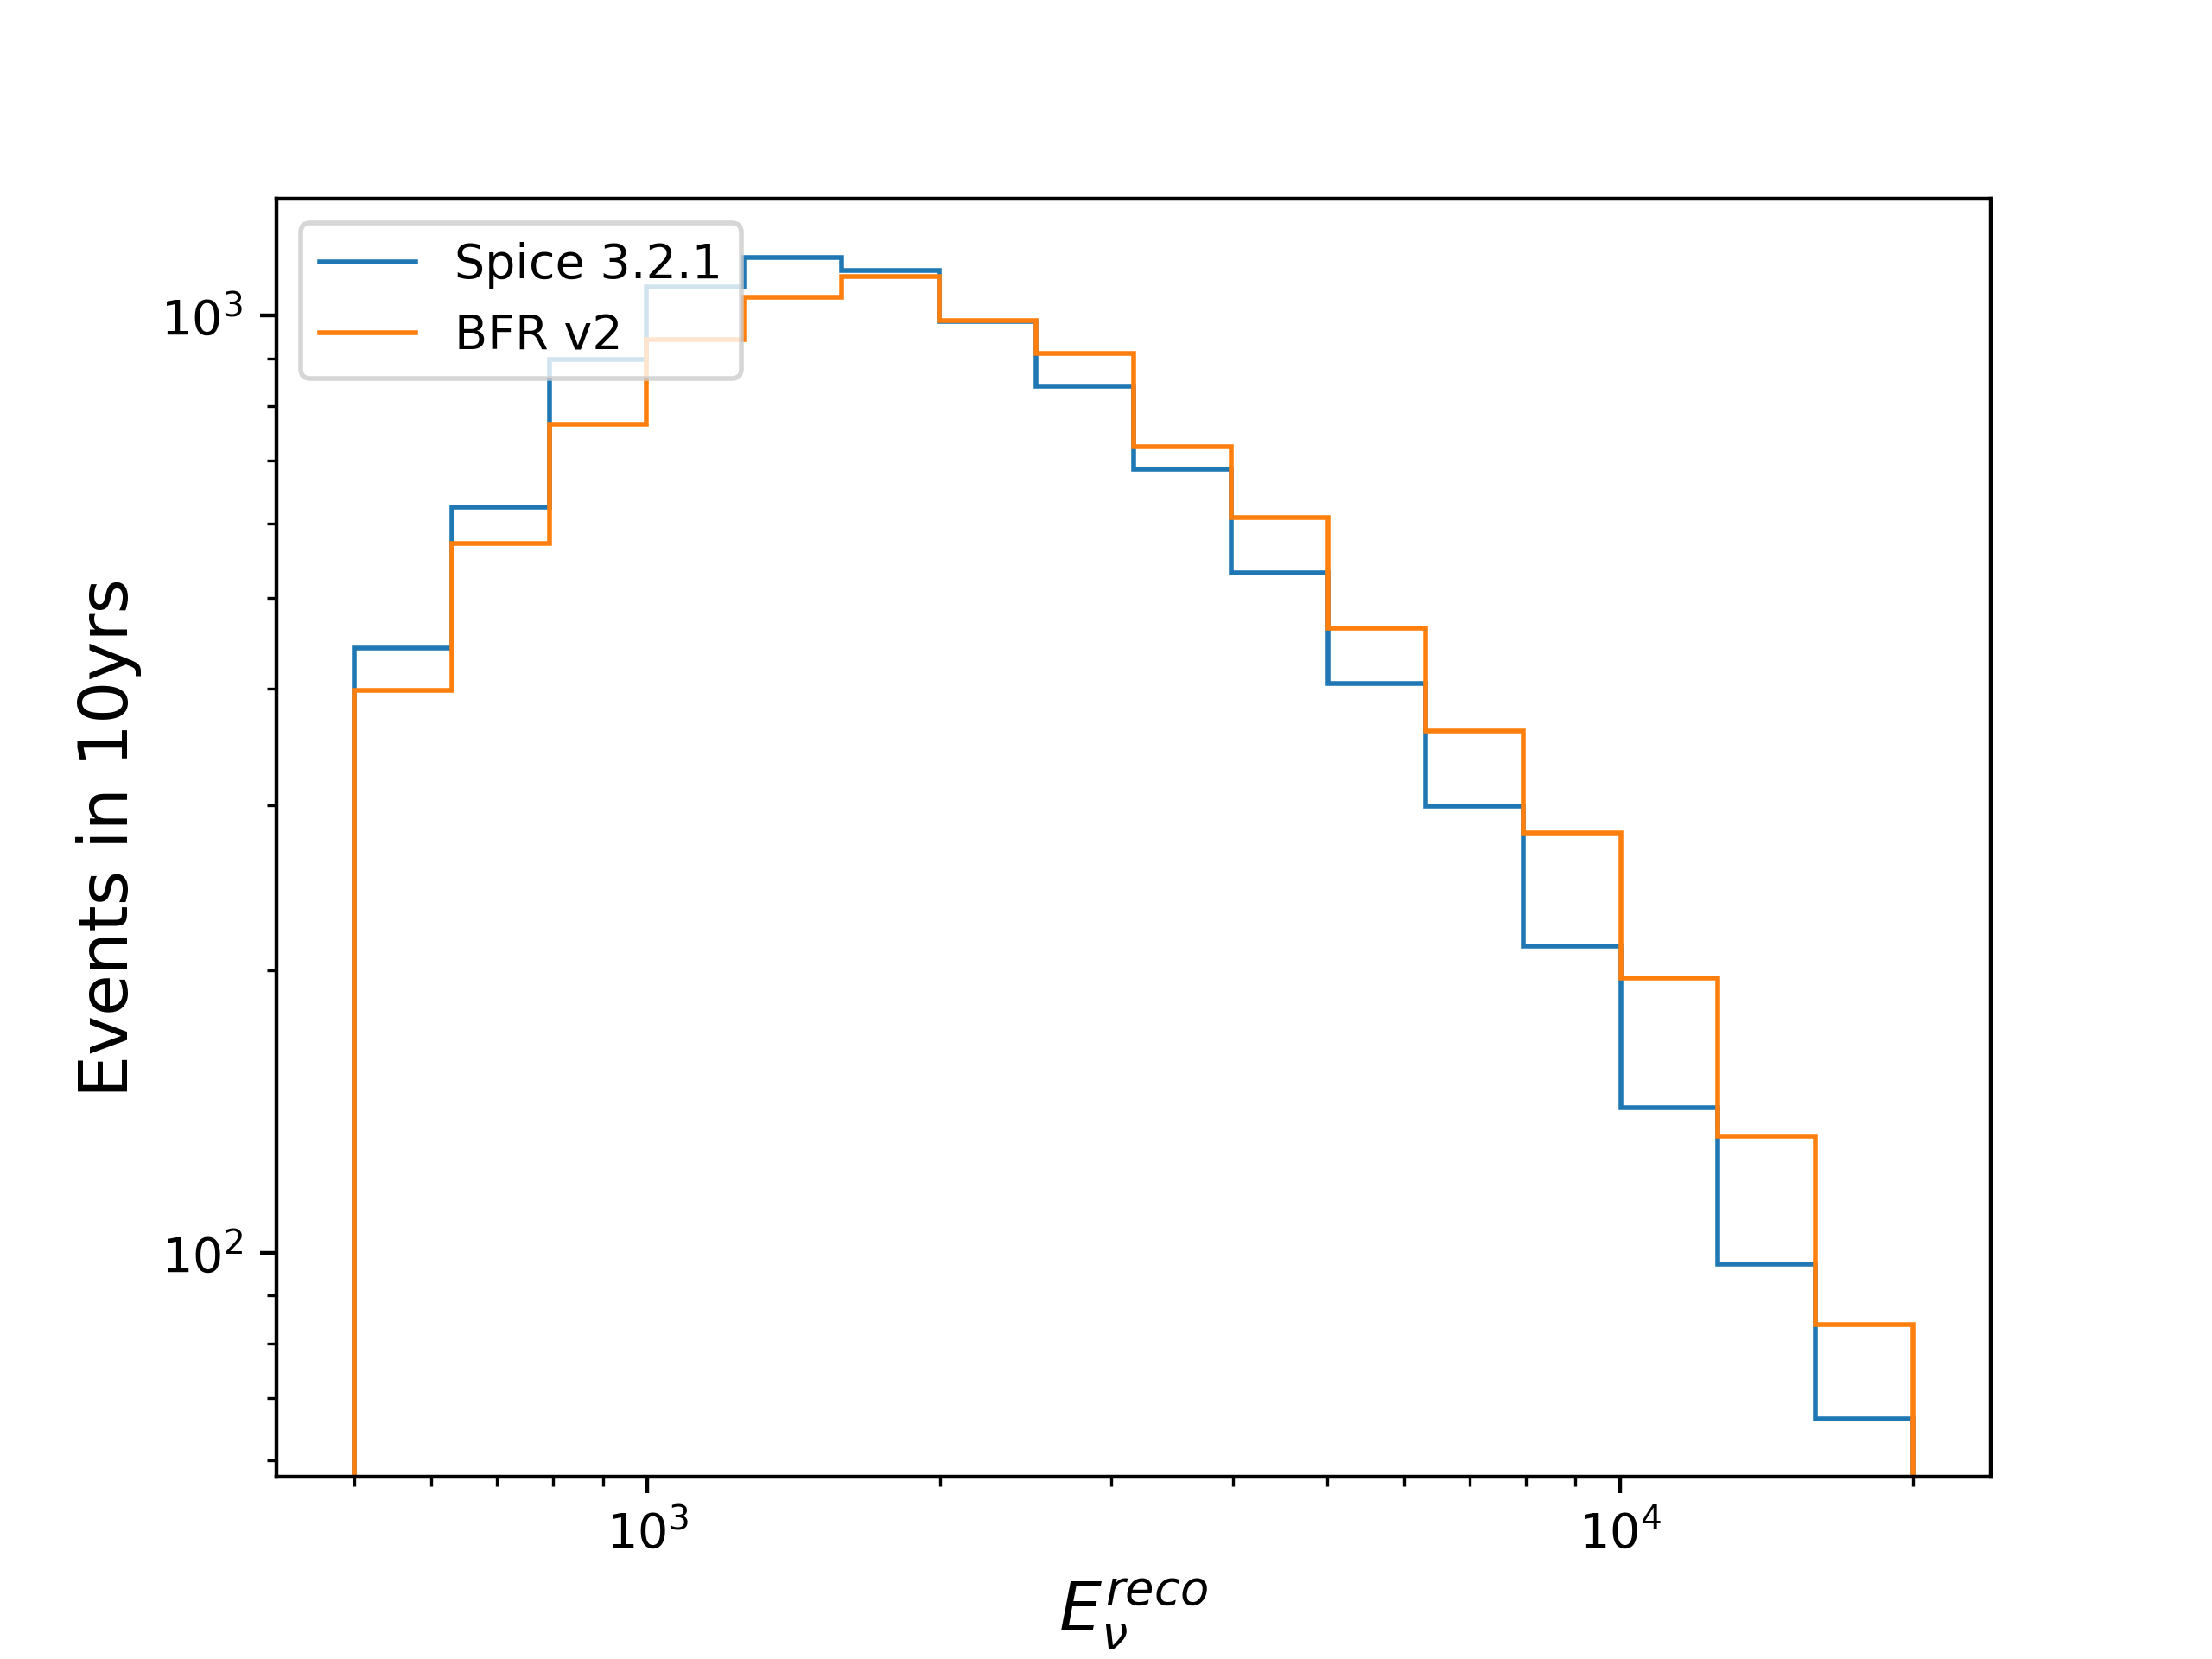
\includegraphics[width=0.45\linewidth]{figures/ice_investigate/reco_energy_distrib_lognorm.png}%
    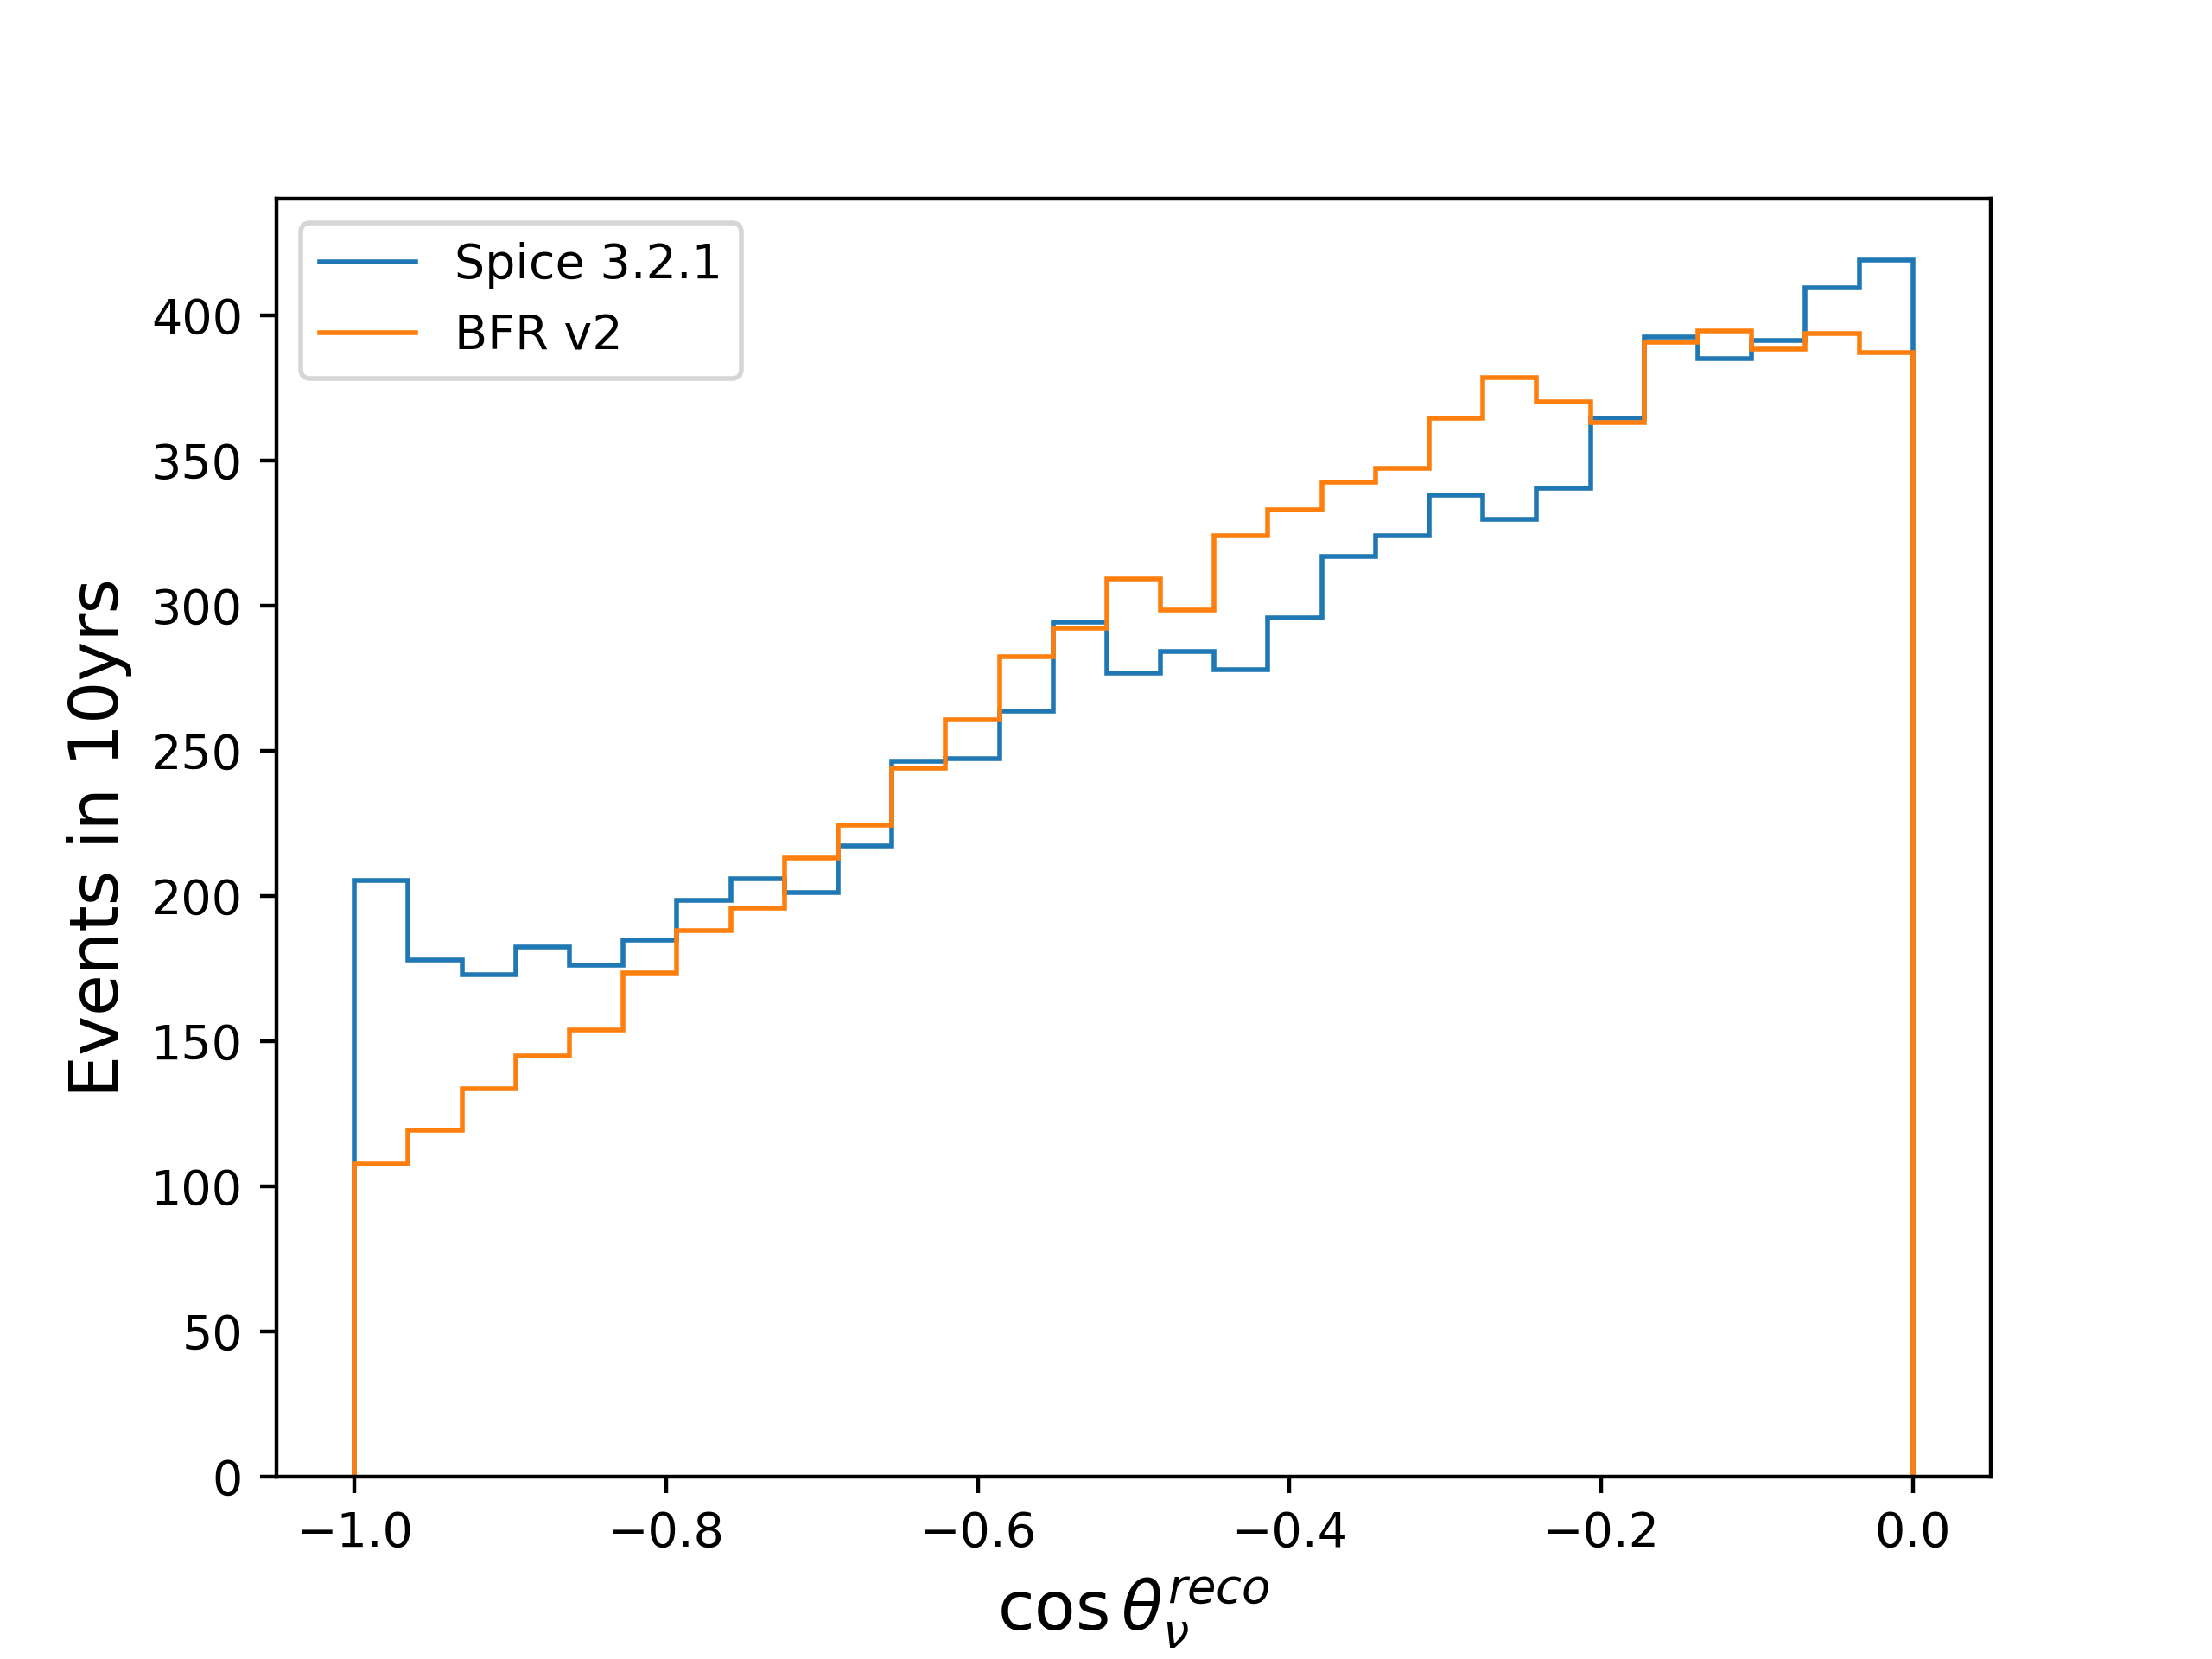
\includegraphics[width=0.45\linewidth]{figures/ice_investigate/true_zenith_distrib.png}
    \caption{The reconstructed energy (zenith) rates are shown in the left (right) comparing Spice 3.2.1 and BFR v2.}\label{fig:bfr_spice_wow}
\end{figure}

\begin{figure}
    \centering
    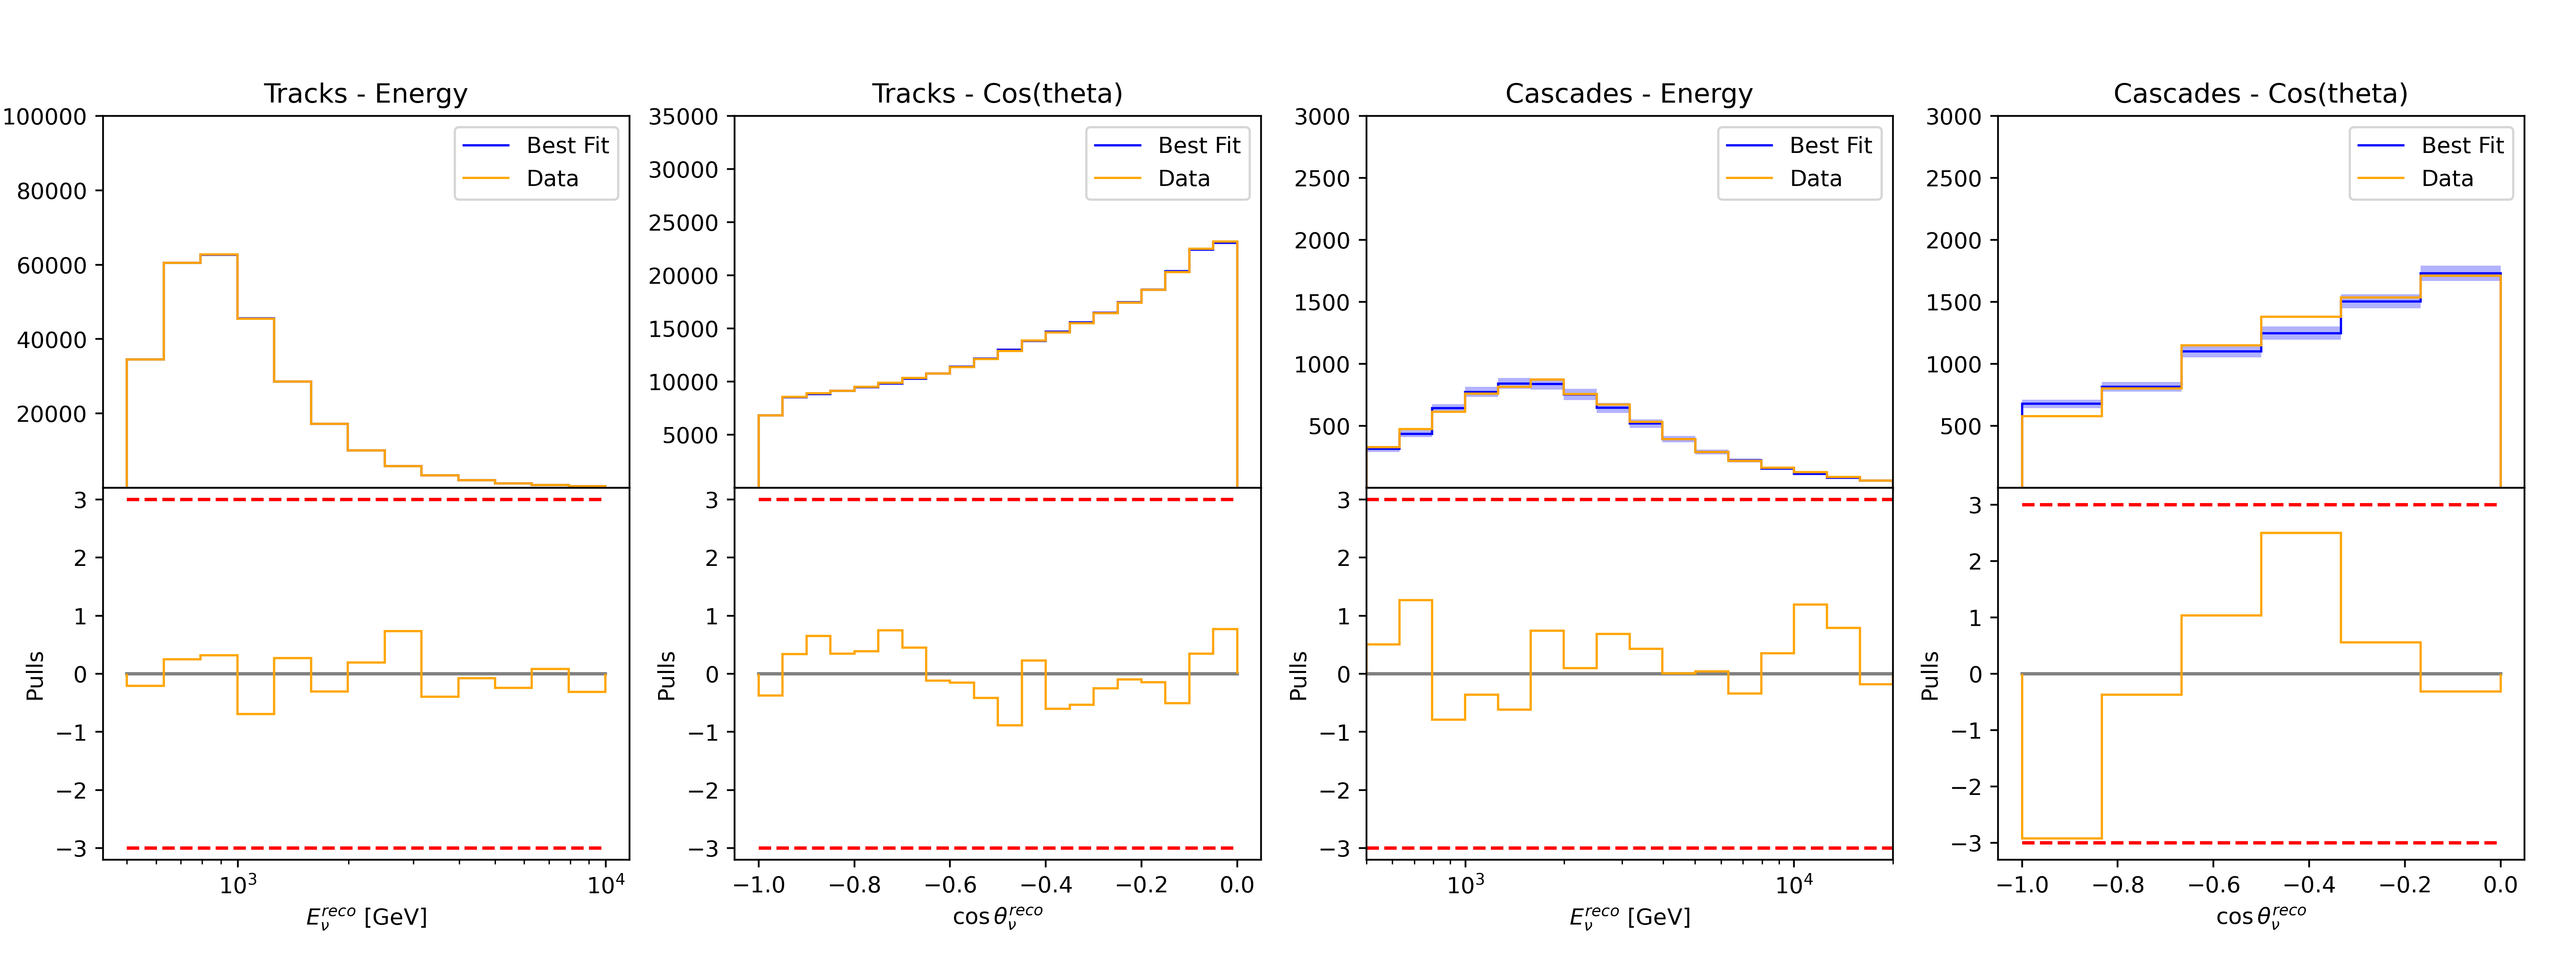
\includegraphics[width=0.8\linewidth]{figures/ice_investigate/goodness_joint_injectbfr_fitspice_Realization_daemon_bfr_Asimov_sterile_0.png}
    \caption{The goodness of fit after injecting a BFR v2-generated realization and fitting with Spice 3.2.1 MC.}\label{fig:icetest_gof}
\end{figure}

\begin{figure}
    \centering
    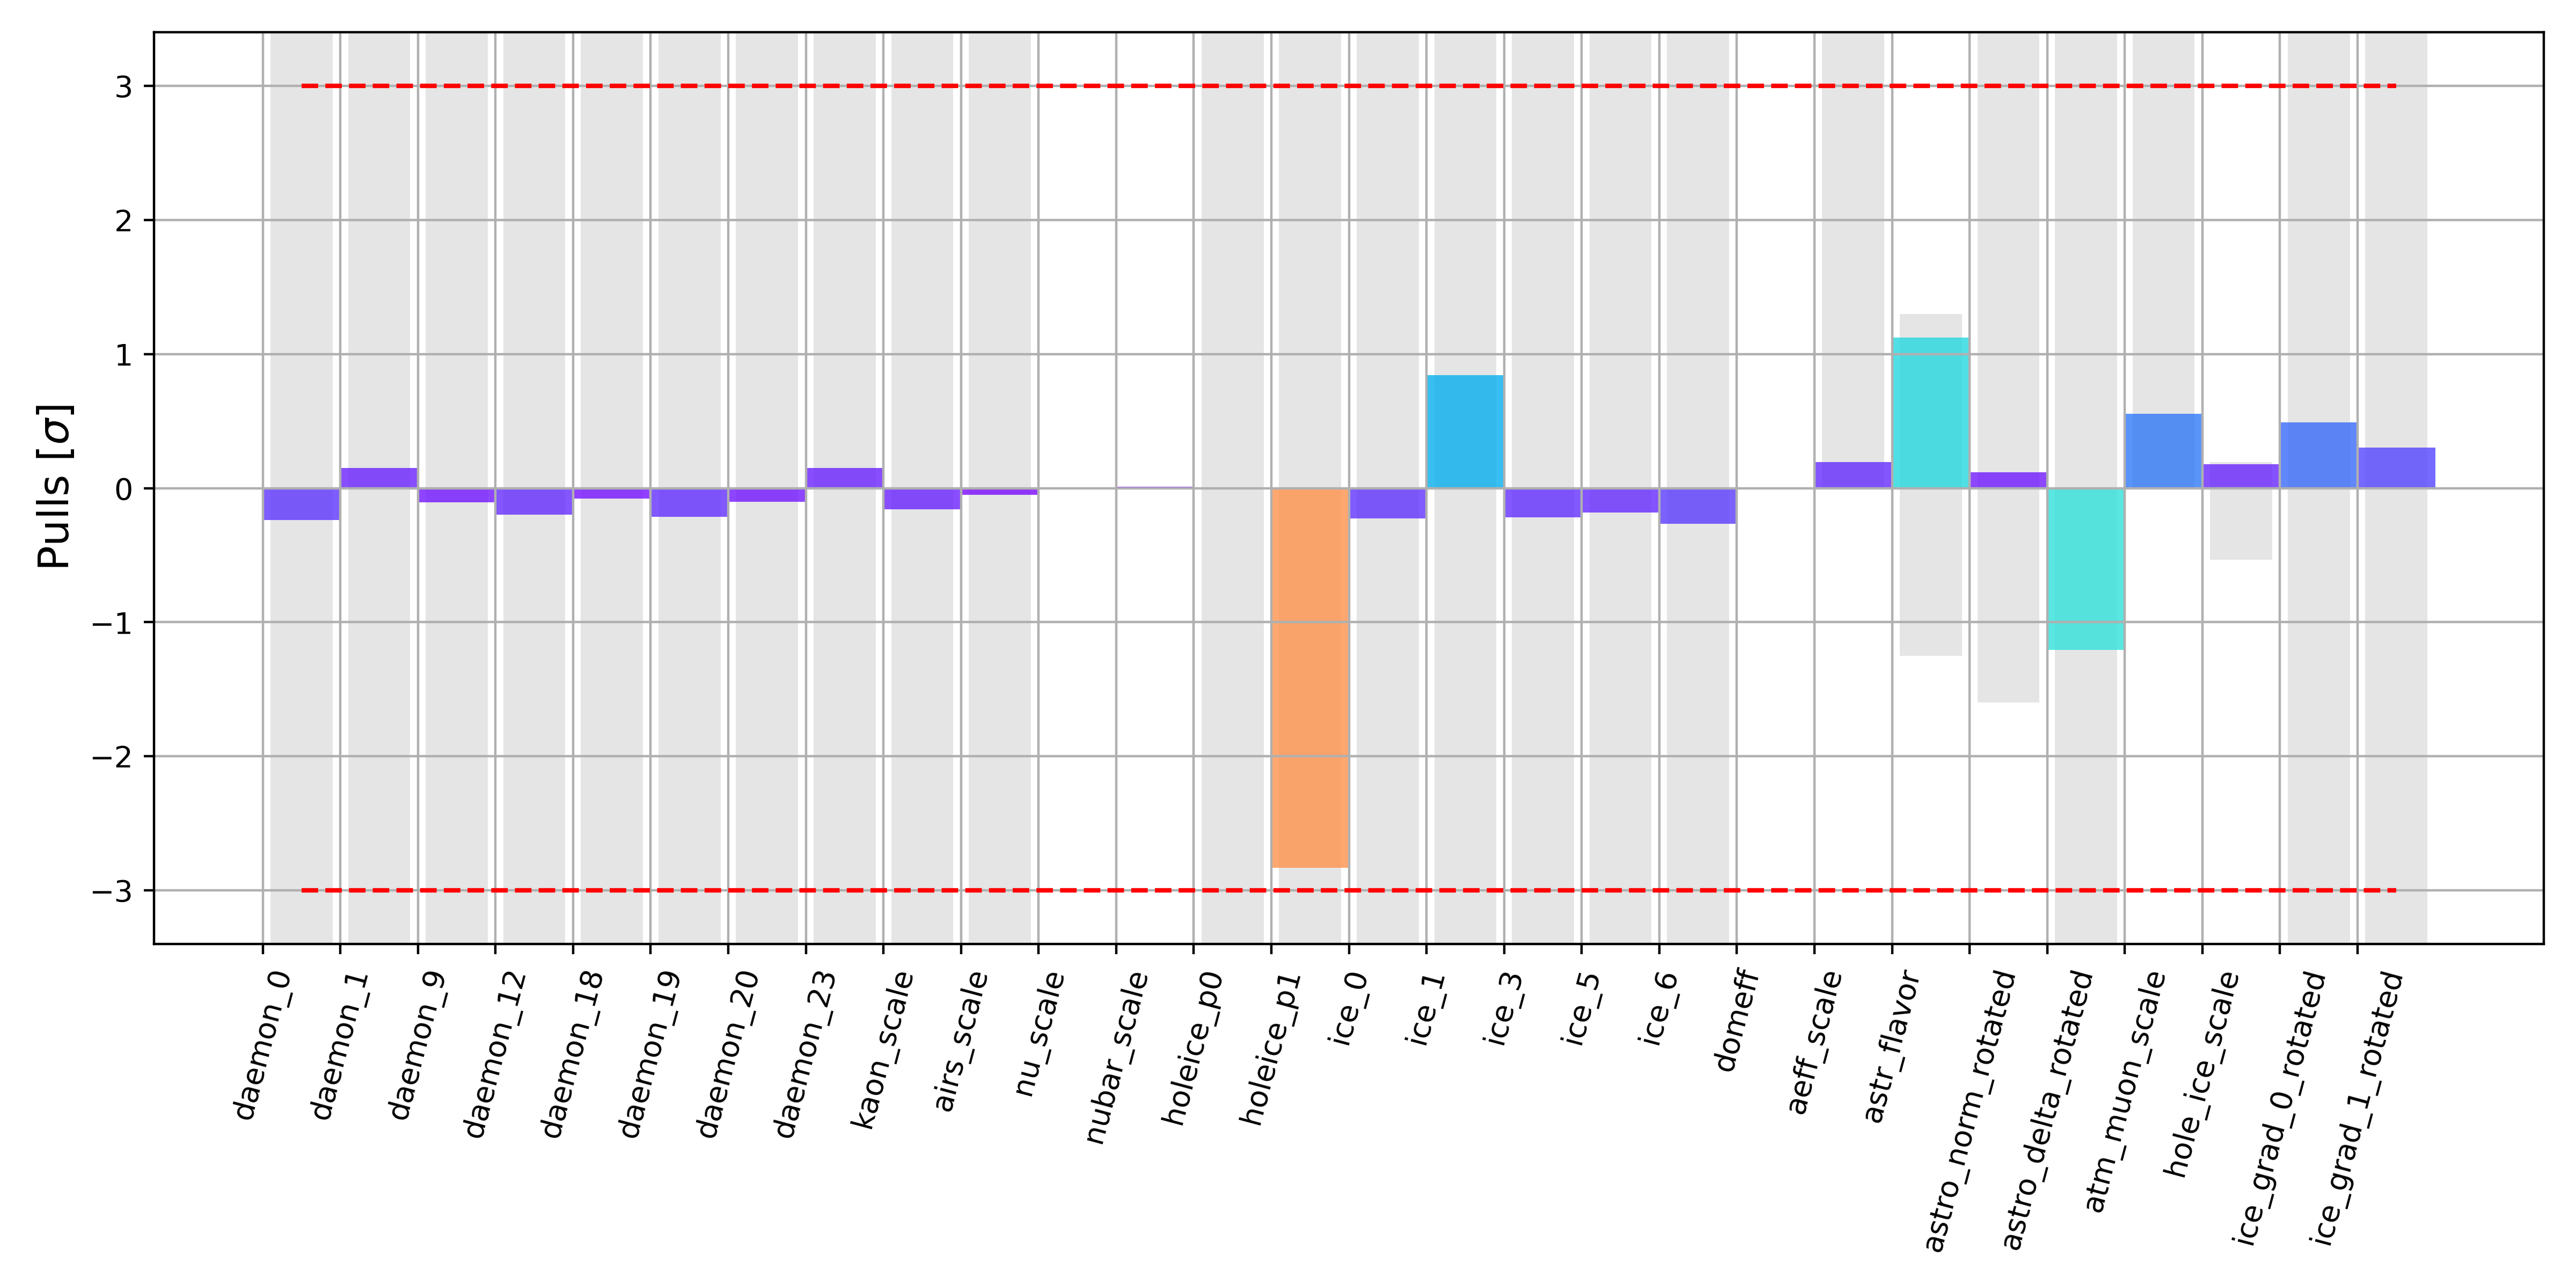
\includegraphics[width=0.7\linewidth]{figures/pulls_Realization_daemon_bfr_Asimov_sterile_0_joint_injectbfr_fitspice.png}
    \caption{90\% CL exclusion contours with three degrees of freedom after injecting BFR v2 and fitting with Spice 3.2.1.}\label{fig:injectbfr_fitspice}
\end{figure}

As the MC predictions begin to deviate at approximately -0.8, shown in Figure~\ref{fig:bfr_spice_wow}, the decision was made to cut the first zenith bin in this analysis, while generating a full high-statistics BFR v2 MC.
Our plan is to revise the analysis for publication with the BFR v2 ice model.



\subsection{Post-Cut 100\% Blind Fits}

As a sanity-check, two fit-scans were performed prior to re-running the blind fits with 100\% of the data: an Asimov scan and a signal inject-recover test. 
These are shown in Figure~\ref{fig:new_sense_again_cut}. 
Little change was observed. 
We then calculated the nuisance parameter pulls, the 1D distribution pulls, and then the 2D distribution pulls; these are shown sequentially in Figures~\ref{fig:pulls_100p_cut} through~\ref{fig:2d_100p_distrib_cut}.
No stop conditions were met. 

\begin{figure}
    \centering
    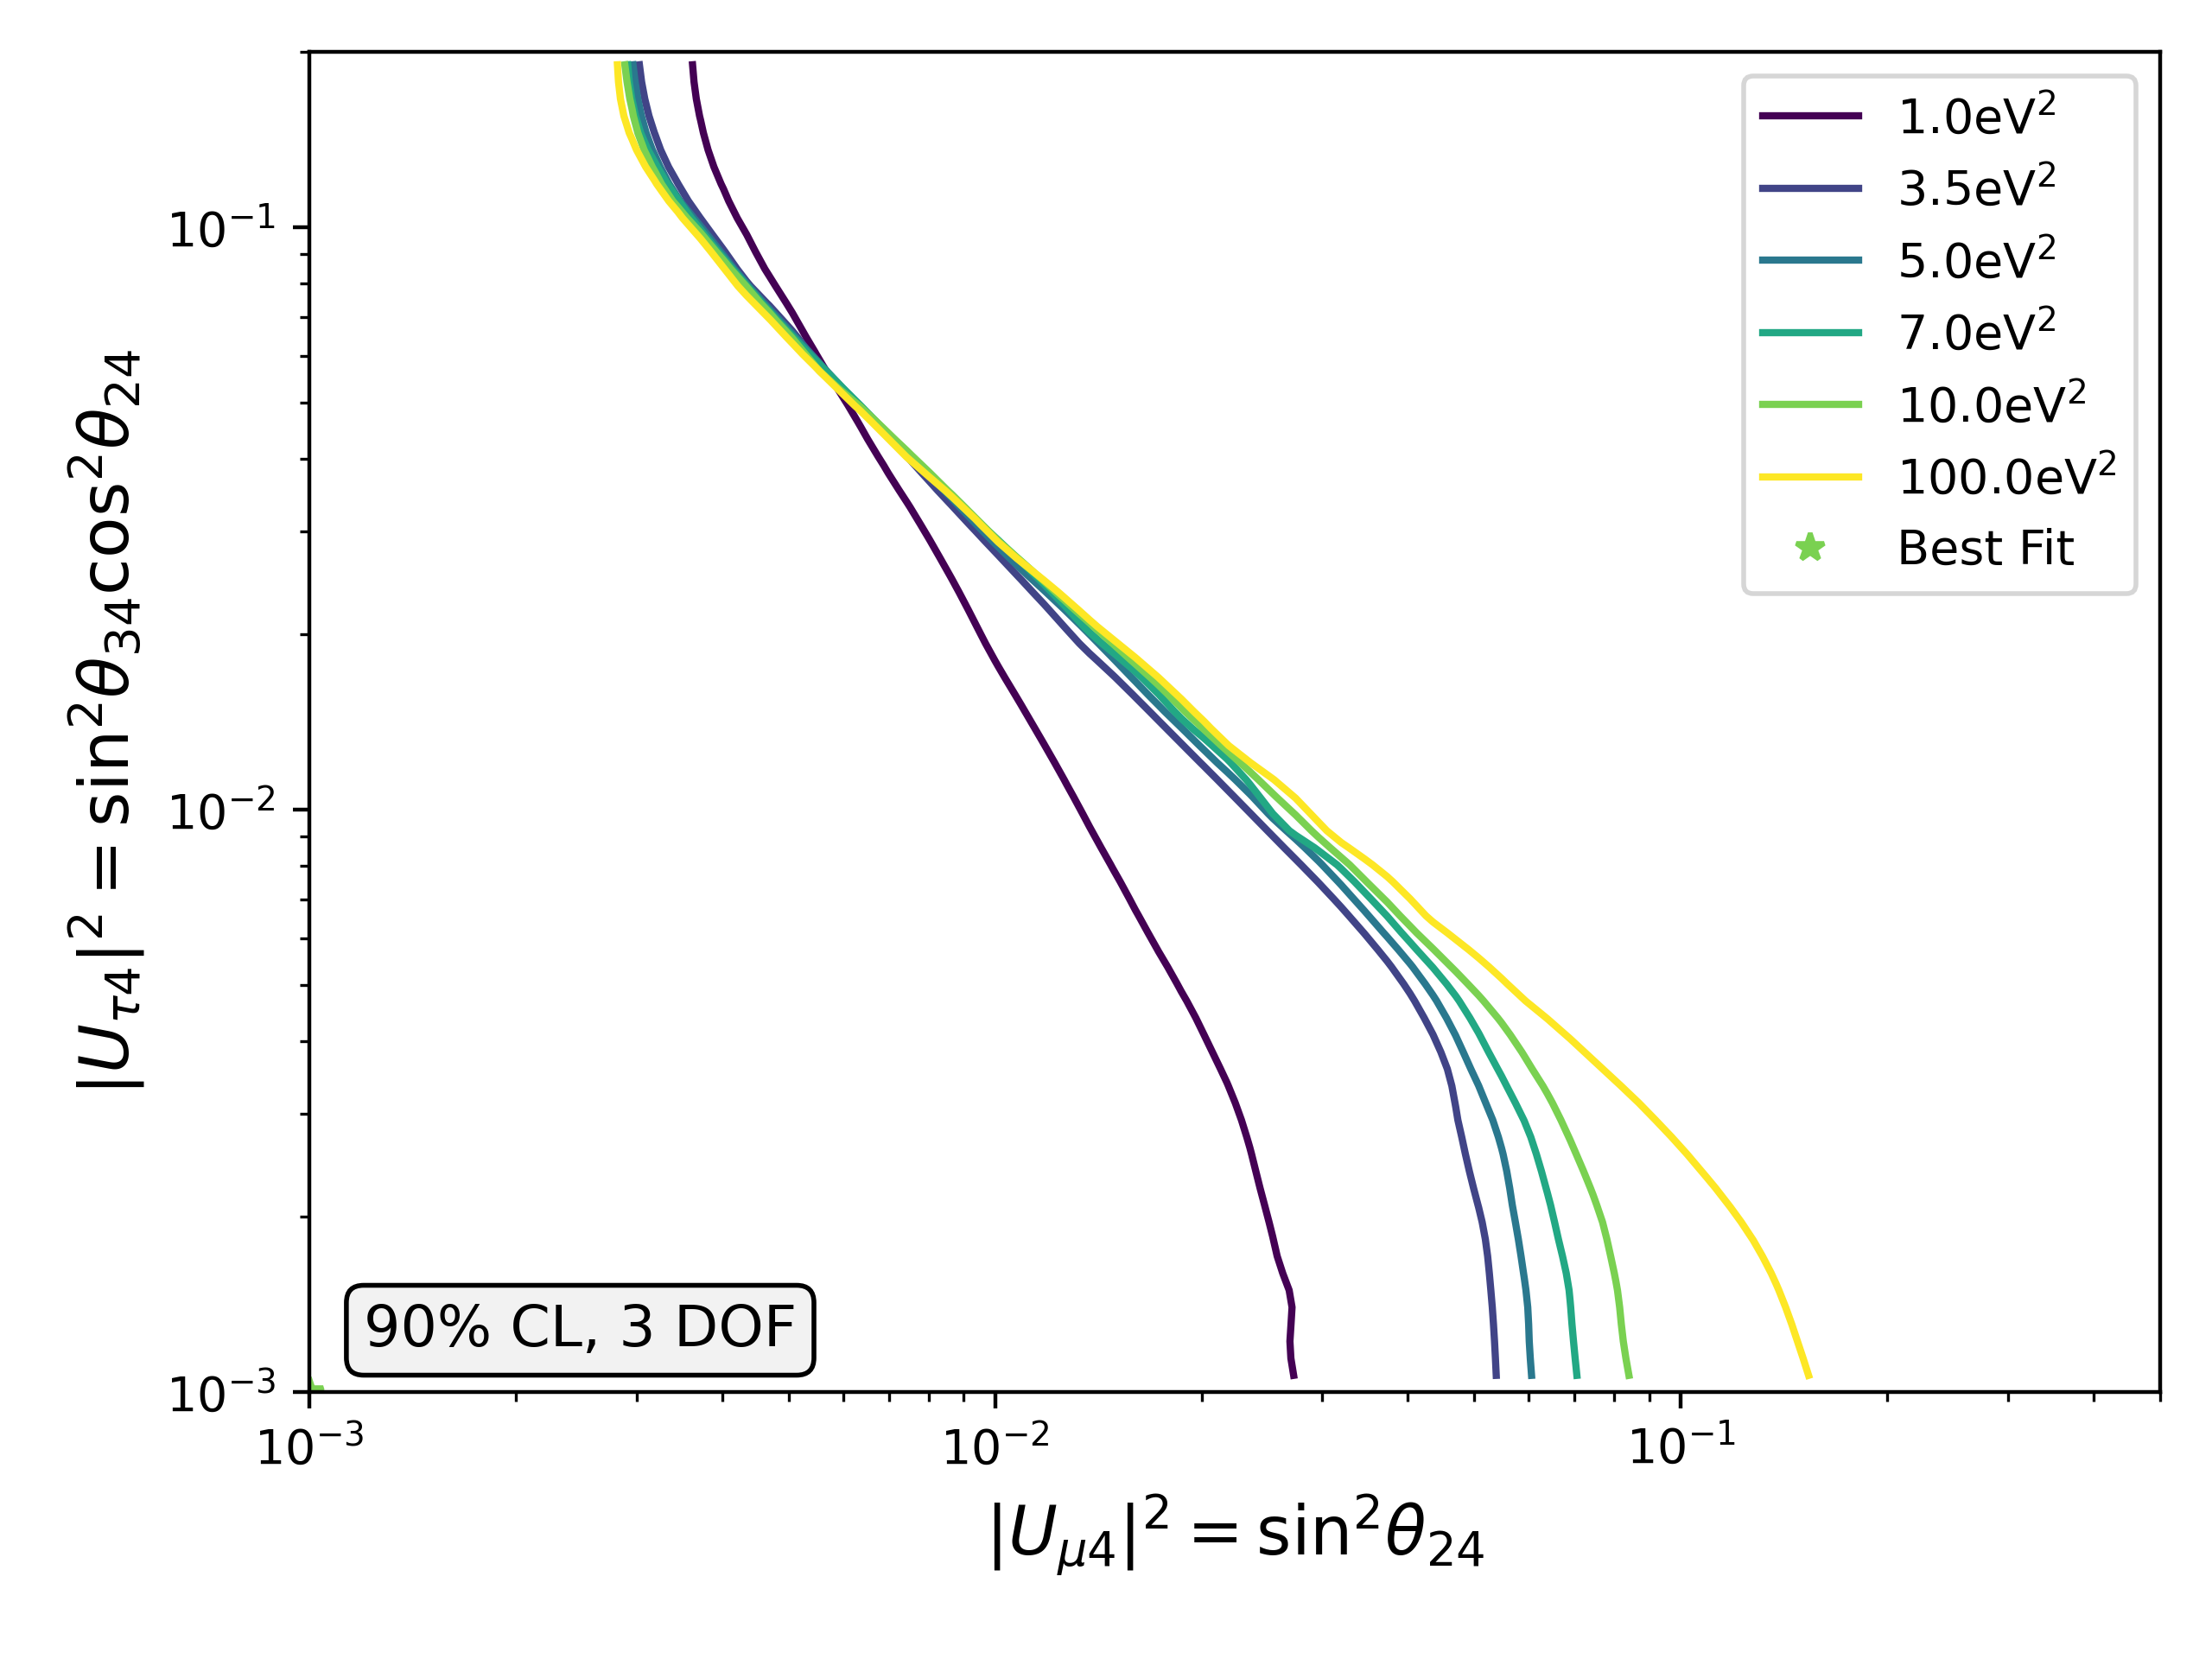
\includegraphics[width=0.45\linewidth]{figures/blindfit/joint_asimov_cut_Realization_daemoncut_Asimov_sterile_0_cl0.9_dof3.png}%
    \includegraphics[width=0.45\linewidth]{figures/blindfit/joint_asimov_cut_signal_Realization_daemoncut_Asimov_sterile_4_cl0.9_dof3.png}
    \caption{Left: the Asimov sensitivity after cutting the up-going zenith bin in the cascade selection; right: the 90\% CL contours after injecting signal and fitting after applying the zenith cut.}\label{fig:new_sense_again_cut}
\end{figure}

\begin{figure}
    \centering
    \includegraphics[width=0.9\linewidth]{./figures/blindfit/pulls_IC86_data_full_cut_joint_data_full_cut.png}
    \caption{The nuisance parameter pulls at the best fit to 100\% of the data after applying the cut.}\label{fig:pulls_100p_cut}
\end{figure}

\begin{figure}
    \centering
    \includegraphics[width=0.9\linewidth]{./figures/blindfit/goodness_joint_data_full_cut_IC86_data_full_cut.png}
    \caption{The 1D pulls and distribution of 100\% of the data after applying the cut.}\label{fig:1d_100p_distrib_cut}
\end{figure}

\begin{figure}
    \centering
    \includegraphics[width=0.9\linewidth]{./figures/blindfit/2dpulls_joint_data_full_cut_IC86_data_full_cut.png}
    \caption{The 2D pulls and distribution of 100\% of the data after applying the cut.}\label{fig:2d_100p_distrib_cut}
\end{figure}


\section{Results}

%The resulting exclusion contours, and best fits, are shown at the 90\% confidence level for the track and cascade subsamples separately in Figure~\ref{fig:final_results_permorpho}. 
Individually, the track and cascade sub-samples show a difference in their preferred minima: the track sample favors a 3+1 model with $\Delta m_{41}^{2}=5.0$ eV$^{2}$, $\abs{U_{\mu 4}}^{2}=0.05$, and $\abs{U_{\tau 4}}^{2}=0.002$ at a significance of $1.2\sigma$ assuming Wilk's theorem and three degrees of freedom; the cascade sample shows no preference for 3+1 over null.
The exclusion contours for each subsample are shown in Figure~\ref{fig:results_separate} for the cascades on the left and tracks on the right. 
The results of the joint fit are shown in Figure~\ref{fig:final_results}, where the data are seen to show a weak preference for the 3+1 model with $\Delta m_{41}^{2}=7$ eV$^{2}$, $\abs{U_{\mu 4}}^{2}=0.03$, and $\abs{U_{\tau 4}}^{2}=0.0$ at a significance of $0.26 \sigma$. 
A comparison is included to the median sensitivities in Figure~\ref{fig:final_results_median}.

\begin{figure}
    \centering
    \includegraphics[width=0.45\linewidth]{figures/multibatch_cascade.png}%
    \includegraphics[width=0.45\linewidth]{figures/multibatch_track.png}
    \caption{On left (right) the 90\% CL exclusion contours with three degrees of freedom from a fit-scan using only the cascade (track) subsample.}\label{fig:results_separate}
\end{figure}

\begin{figure}
    \centering
    \includegraphics[width=0.7\linewidth]{figures/results_joint_data_full_cut_IC86_data_full_cut_cl0.99_dof3.png}
    \caption{Left to right, top to bottom: the exclusion contours for three degrees of freedom and at a confidence level of 90\%, 95\%, and 99\%. The best fit is at $\Delta m_{41}^{2}=7$ eV$^{2}$, $\abs{U_{\mu 4}}^{2}=0.03$, and $\abs{U_{\tau 4}}^{2}=0.0$.}\label{fig:final_results}
\end{figure}

\begin{figure}
    \centering
    \includegraphics[width=0.7\linewidth]{figures/results_with_median.png}
    \caption{The results of the joint analysis overlain on top of the median sensitivities at the 95\% confidence level.}\label{fig:final_results_median}
\end{figure}

Exclusion contours are also shown assuming two degrees of freedom at the 90\% confidence level in comparison to results from Super-K and IceCube DeepCore in Figure~\ref{fig:comparison_results}. 
The results presented in this analysis are the strongest constraints with three degrees of freedom for $\abs{U_{\mu 4}}^{2}$ and $\abs{U_{\tau 4}}^{2}$ to date. 


\begin{figure}
    \centering
    \includegraphics[width=0.7\linewidth]{./figures/result_comparison.png}
    \caption{The 90\% confidence level results for this analysis with two degrees of freedom at $\Delta m_{41}^{2}=$ 1.0 eV$^{2}$. Sensitivities from DeepCore~\cite{Aartsen_2017_dc} and Super-K~\cite{PhysRevD.91.052019} at 1.0eV$^{2}$ are provided for comparison.}\label{fig:comparison_results}
\end{figure}    

\iffalse
\begin{figure}
    \centering
    \includegraphics[width=0.6\linewidth]{figures/cascade_data_full_cut_moreseed_IC86_data_full_cut_cl0.9_dof3.png}\\
    \includegraphics[width=0.6\linewidth]{figures/cascade_data_full_cut_moreseed_IC86_data_full_cut_cl0.9_dof3.png}
    \caption{On top (bottom), the exclusion contours from fits to the cascade (track) sub-sample individually. The best fit is at $\Delta m_{41}^{2}=7$ eV$^{2}$, $\abs{U_{\mu 4}}^{2}=0.03$, and $\abs{U_{\tau 4}}^{2}=0.0$.}\label{fig:final_results_permorpho}
\end{figure}
\fi

\chapter{Discussion \& Conclusions}\label{chapter:end}

\section{Discussion}

What we have found is that the introduction of the cascades to the track analysis weakens the disappearance signature seen previously.
There are also no strong signatures of appearance or disappearance in the cascades channel, and as a consequence further tensions may arise. 
While future work will implement the newer ice model with birefringence in the nominal expectation for the final results of this analysis, if these discrepancies persist then this would suggest that the track and cascade samples may not be jointly described by a common set of nuisance parameters.
And if the lack of strong cascade appearance persists after the ice model updates, then we may find these results to fall into tension with predictions of strong $\nu_{e}/\nu_{\tau}$ appearance consistent with the BEST best fit sterile hypothesis.  

We have also found weaker constraints compared to previous analyses using the same event selection~\cite{Aartsen_2020, Aartsen_2020_prd}.
One noteable change from previous analyses was a switch from a conventional flux model using Hillas-Gaisser H3a~\cite{GAISSER2012801}, SIBYLL 2.3c~\cite{Riehn:2017mfm}, and the Barr parametrization~\cite{PhysRevD.74.094009} to daemonflux~\cite{yanez2023daemonflux}.
In Section~\ref{fig:flux_mismod} we had shown that if daemonflux is a better description of the truth, then by using the older model one could expect spurious signatures of sterile neutrino oscillations. 
Knowing this it is reasonable to expect that the previously observed signatures might weaken in this updated search. 
This is not to say that no such 3+1 signal-like feature exists in IceCube data, however: more recent results\footnote{as of writing currently under internal paper review} using an updated event selection and reconstruction along with daemonflux have found even stronger results for 3+1 sterile neutrinos~\cite{alfonso_slides} that are consistent with the best-fit point of this analysis.

\iffalse


The disagreement in best fits between the tracks and cascades is also possibly related to the observed data/MC disagreements seen in the cascade channel. 
We showed in Section~\ref{sec:ice_chaos_ohgod} that birefringence in the ice has a large effect on the reconstructed angular quantities for cascades. 
In the case where a birefringent ice model was injected as the truth, the joint fits showed a stronger preference for the null model than what is predicted for median sensitivities. 
This comparison is shown below in Figure~\ref{fig:median_mismod}.
And so if birefringence is a better description of the ice then by fitting assuming the older Spice model, even without the cut bin, the addition of cascades could weaken the significance of a track-only result when fit jointly. 
\begin{figure}
    \centering
    \includegraphics[width=0.9\linewidth]{figures/mismodel_median_sense_cl0.9.png}
    \caption{The median sensitivities at 90\% CL with the results of an inject-BFR, fit Spice, mismodeling test overlain in red. The mismodeling results lie just outside the 68\% bounds and in some places reach the bounds of the 95\%.}\label{fig:median_mismod}
\end{figure}
\fi

\section{Conclusions}

Numerous oscillations persist in neutrino oscillations today: many of which can be solved through additional eV$^{2}$-scale oscillations. 
Such an additional neutrino could not interact weakly in order to be consistent with measurements of Z-boson decay, and so is described as ``sterile.''
Through attempts to test such explanations using sterile neutrinos, several tantalizing signal-like hints have been observed with varying degrees of significance in both $\nu_{e}/\bar{\nu}_{e}$ disappearance and $\nu_{\mu}$ disappearance; including the 8-year IceCube matter-enhanced sterile neutrino oscillations study in which signal-like hints above the 90\% confidence level for the 3+1 light sterile neutrino model were found.

Here, we have presented the first results of a joint track-cascade analysis combining the methods used in previous IceCube analyses along with novel methods developed to needed to handle the additional sources of systematic uncertainty introduced with this new event morphology. 
We have probed $\abs{U_{\mu4}}^{2}$ and $\abs{U_{\tau4}}^{2}$ through high-energy events in a search the first time, implemented a new conventional flux model and an updated bulk ice model with an improved system for covariance matrix calculation, and introduced a new starting event sample. 
Results presented here improve upon world-leading constraints in $U_{\mu4}$-$U_{\tau4}$ parameter space, and have opened the door for large-volume \v{C}erenkov neutrino experiments to directly probe the models preferred by experiments like BEST.

Because of challenges in ice modeling, immediate work will focus on the re-simulation of Monte Carlo to update the nominal ice model from Spice 3.2.1 to BFR v2: one which fully accounts for the effects of birefringence in ice.
We may then find that the disagreement between the track, cascade, and joint fits persist; this would suggest that the cascade and track samples are not sufficiently described by a common set of nuisance parameters, and further investigation would be of merit. 
We may instead find a consistent description of sterile neutrinos in both event morphologies: laying the foundations for an even stronger and compelling test of the 3+1 sterile neutrino oscillation model with IceCube.

\end{document}